% \iffalse meta-comment
%  rubikcube.dtx
% 
%  version v5.0  (February 25, 2018)  
%
%  Copyright 2018 
%  RWD Nickalls (dick@nickalls.org) and 
%  A Syropoulos (asyropoulos@yahoo.com)
%
% This work may be distributed and/or modified under the
% conditions of the LaTeX Project Public License, either version 1.3
% of this license or (at your option) any later version.
% The latest version of this license is in
%   http://www.latex-project.org/lppl.txt
% and version 1.3 or later is part of all distributions of LaTeX
% version 2005/12/01 or later.
%
%
% This work consists of the files rubikcube.dtx and rubikcube.ins
% and the derived file rubikcube.sty.
%
%<*readme> 
%
% The rubikcube package provides a collection of LaTeX commands and macros 
% for the typesetting of Rubik cube configurations and rotation 
% sequences using the TikZ graphic language.
%
% Please report errors or suggestions for improvement to
%
%         Dick Nickalls or Apostolos Syropoulos
%
% This package requires the basic TikZ package to be loaded already
%</readme>
%
%<*driver>
\listfiles
\documentclass{ltxdoc}
\IfFileExists{rubikcube.sty}{\usepackage{rubikcube}}{%
    \GenericWarning{rubikcube.dtx}{Package file rubikcube.sty not found.
    Documentation will be messed up!^^J
    (Generate rubikcube.sty by (La)TeXing rubikcube.ins, and then^^J
    process rubikcube.dtx again)^^J}\stop
}%
\pagestyle{myheadings}
\markright{\texttt{rubikcube} \ \ (Rubik bundle v5.0, 2018) \ \ \texttt{www.ctan.org/pkg/rubik}}
\usepackage{ifpdf}
\usepackage{url,path}  %% for references
\usepackage{supertabular} %% for Notation table
\usepackage{hypdoc}    %% for hyperref documenting of LaTeX packages
%%\OnlyDescription
\EnableCrossrefs
\PageIndex
\CodelineIndex
\CodelineNumbered
\RecordChanges
\setcounter{StandardModuleDepth}{1}
\begin{document}
  \DocInput{rubikcube.dtx}
  \PrintChanges
  \PrintIndex
\end{document}
%</driver>
% \fi
%
%
% 
%%% \CheckSum{6231} 
%
%%% \CharacterTable
%%  {Upper-case    \A\B\C\D\E\F\G\H\I\J\K\L\M\N\O\P\Q\R\S\T\U\V\W\X\Y\Z
%%   Lower-case    \a\b\c\d\e\f\g\h\i\j\k\l\m\n\o\p\q\r\s\t\u\v\w\x\y\z
%%   Digits        \0\1\2\3\4\5\6\7\8\9
%%   Exclamation   \!     Double quote  \"     Hash (number) \#
%%   Dollar        \$     Percent       \%     Ampersand     \&
%%   Acute accent  \'     Left paren    \(     Right paren   \)
%%   Asterisk      \*     Plus          \+     Comma         \,
%%   Minus         \-     Point         \.     Solidus       \/
%%   Colon         \:     Semicolon     \;     Less than     \<
%%   Equals        \=     Greater than  \>     Question mark \?
%%   Commercial at \@     Left bracket  \[     Backslash     \\
%%   Right bracket \]     Circumflex    \^     Underscore    \_
%%   Grave accent  \`     Left brace    \{     Vertical bar  \|
%%   Right brace   \}     Tilde         \~}
%
%
% \title{%
%       \ifpdf\pdfbookmark[1]{Title}{Title}\else\fi%
%        The \textsc{rubikcube} package}
%
% \author{
%      RWD Nickalls (dick@nickalls.org) \\
%     A Syropoulos (asyropoulos@yahoo.com)
%       }
%  \date{This file describes version \RCfileversion\ (\RCfiledate)\\
%   \texttt{www.ctan.org/pkg/rubik}}
%  \maketitle
%
%  \begin{abstract}
%  The \rubikcube\ package provides LaTeX commands and macros 
%  for  typesetting  Rubik cube (3x3x3) notation,  configurations, and 
%  rotation sequences  using the  TikZ graphic language. It is part of the 
%   Rubik `bundle'.
%  \end{abstract}
%
% \medskip
%
% \begin{minipage}{11cm}
% \centering
% \ifpdf
%  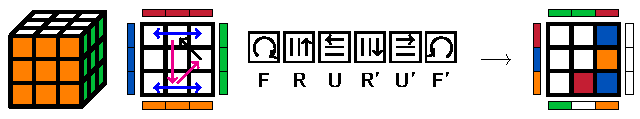
\includegraphics[width=10cm]{rubik-doc-figF.pdf}
% \else
% \fi
% \end{minipage}
%
%  \tableofcontents
%
% \pagebreak
%
% \section{Introduction}
%
% The  \rubikcube\  package (part of the \textsc{rubik} `bundle') provides  a 
% collection of \LaTeX\ commands 
% and macros for  typesetting  Rubik cube (3x3x3) configurations  using the  
% PGF/TikZ graphic languages. 
% We have extended  the  rotation  hieroglyph notation,  originally  
% developed  by Garfath-Cox (1981), and improved by Duvoid (2010, 2011).
%
% The \rubikcube\ package is  the `base' package of the bundle, and is required by all of 
% the Rubik packages; it deals  primarily with  typesetting 3x3x3 cube (Rubik cube)
%  configurations.
% The \textsc{rubikrotation} package processes  rotation sequences  and keeps  track of 
% the cube's configuration during rotations.
% The \textsc{rubikpatterns} package is a small database of 3x3x3  (Rubik) cube rotation 
% sequences  which generate well-known named cube configurations (patterns).
% The \textsc{rubiktwocube} package  allows the typesetting of  2x2x2 cube (Two cube) 
% configurations. 
%
% Full 3x3x3 functionality requires the following  packages to be  loaded 
% (TikZ first; \textsc{rubikcube} second), as follows: 
%\begin{verbatim}
%  \usepackage{tikz}
%  \usepackage{rubikcube,rubikrotation,rubikpatterns}
%\end{verbatim}
% Full 2x2x2 functionality requires the \textsc{rubiktwocube} package \textit{in addition} to the 
%  packages listed above.
% Note that the \verb!TikZ! package must be loaded \textit{before} the \textsc{rubikcube} 
% package.
%
%  The \rubikcube\ package has been road-tested  on a Microsoft 
%  platform (with \textsf{MiK}\TeX), a GNU-Linux platform (Debian 8.2.0 
%  and {\TeX}Live 2017), and on a Solaris platform (OpenIndiana).
%
% 
% For the mathematics and group theory associated with the   Rubik cube  see Chen~(2004), 
% Davis (2006), Fung website, Golomb~(1981, 1982),  Hofstadter (1981), Hutchings~(2011), 
% Heise website, Joyner~(2008), Kociemba website, 
% Rokicki~\textit{et al.} (2013), Scherphius website,  Tran~(2005).
%  Other useful websites are the Speedsolving website, and  those 
% maintained  by Duvoid,  by Fridrich, by Jelinek,  by Reid, and by Vandenburgh. 
%  A useful online solver utility (based on an algorithm by Kociemba) is
% available at the RuWix website. Websites with good pages on  patterns and symmetries are 
% those by  Fridrich, Kociemba, Longridge, Reid, Randelshofer, Scherphius 
% (see References for details). 
%
% For historical and technical details  regarding Rubik's cube see Sher (2014), 
% and also the Wikipedia article \textit{Rubik's Cube}.
%
%
%      \subsection{Requirements}
%
%  The \rubikcube\ package requires the TikZ package, since it makes  
%  use  of the TikZ picture environment and the \cmd{\pgfmathsetmacro} command.
% Consequently, the \verb!TikZ! package must be loaded \textit{before} 
% the \textsc{rubikcube}  package.
%  The \textsc{rubikrotation}  package (see below) 
% requires  Perl to be installed.
%
%
%  \subsection[rubikrotation package]{Supporting  tool---the 
%   \textsc{rubikrotation} package}
%   \label{sec:rubikrotation}
%
%  The \textsc{rubikrotation} package (also part of the \textsc{rubik} `bundle'), 
%  is a dynamic extension to  the \rubikcube\ package. It consists of  the  
% Perl program  \texttt{rubikrotation.pl}  and the associated  style option
%  \texttt{rubikrotation.sty}. 
%  The \textsc{rubikrotation} package  implements rotation sequences on-the-fly using a
%   \cmd{\RubikRotation}\marg{rotation-sequence} command. It returns the 
%  new state in a form which can then be used by the \rubikcube\ package.
% It also returns some useful strings associated with the rotation sequence 
% which can  be used by the \rubikcube\ 
% package---see also Section~\ref{sec:showsequence}.
%
%  Since the  \cmd{\RubikRotation} command works by \textsc{call}ing the  
%  \texttt{rubikrotation.pl} program, it follows that the \textsc{rubikrotation}
%   package requires  (a)~Perl to be installed, 
%  and (b)~the \LaTeX\ engine  needs to be run using the  \texttt{--shell-escape} 
%  command-line option. Those wishing to use Lua\LaTeX\  will also need to have access 
% to the  \texttt{shellesc} package (this can always be downloaded from CTAN directly).
%  See the \textsc{rubikrotation}  documentation for further details.
% See also the examples in the file \texttt{RubikExamples.pdf}.
%
%
%
%  \subsection[rubikpatterns]{Supporting  database---\textsc{rubikpatterns} package }
%  \label{sec:patterns}
%
%  
%  The \textsc{rubikpatterns.sty} file (also part of the \textsc{rubik} `bundle')
%  is a small database of some well-known 3x3x3 cube (Rubik cube) rotation sequences, 
% stored as  named macros. For~example, the `fourspot' and `sixspot' sequences are encoded in 
% this package as follows:
%\begin{verbatim}
%  \newcommand{\fourspot}{[fourspot],F2,B2,U,Dp,R2,L2,U,Dp,<(12q*, 8f*)>}
%  \newcommand{\sixspot}{[sixspot],U,Dp,R,Lp,F,Bp,U,Dp,<(8q*, 8f*)>}
%\end{verbatim}
%  These sequences  can be  processed by name (using the  \cmd{\RubikRotation} command
%  which also requires Perl to be installed---see Section~\ref{sec:rubikrotation}), and 
% then displayed (using the \cmd{\ShowCube} command in conjunction with various 
%  \cmd{\DrawRubikCube...} commands). So, for~example, one could typeset the so-called 
%  `fourspot' configuration using the following code:
%\begin{verbatim}
%  \usepackage{tikz,rubikcube,rubikrotation,rubikpatterns}
%  ...
%  \RubikCubeSolved
%  \RubikRotation{\fourspot} % this runs the Perl program \texttt{rubikrotation.pl}
%  \ShowCube{2.4cm}{0.6}{\DrawRubikCubeRU}
%\end{verbatim}
% The sequence itself can be readily typeset using the \cmd{\ShowSequence} command
% (see Section~\ref{sec:showsequence}). 
% See also the \textsc{rubikrotation}  documentation---especially
% Section~5.1.1 \textit{Sequences as macros}. 
% See also the examples in the file \texttt{RubikExamples.pdf}.
%
%
%
%  \subsection[rubiktwocube]{Supporting 2x2x2 package---\textsc{rubiktwocube} package }
%  \label{sec:patterns}
%
%  The \textsc{rubiktwocube} package carries the macros and commands necessary 
%  for processing and displaying  2x2x2 cubes (TwoCubes). The 2x2x2 commands are isomorphic
%  with the 3x3x3 commands---i.e.,~the word `\texttt{Two}' has  replaced  the 
%  word `\texttt{Rubik}' in commands.
%  Consequently, users of this package will need to be familiar with the \textsc{rubikcube} package.
%  There are lots of 2x2x2  examples in the file \texttt{RubikExamples.pdf}.
%  
%
%  \subsection{Copyright}
%  Copyright 2014--2018 RWD Nickalls and A Syropoulos.
%
% \medskip
% {\noindent}This work may be distributed and/or modified under the
% conditions of the LaTeX Project Public License, either
% version 1.3c of this license or any
% later version. The latest version of this licence is in 
%  |www.latex-project.org/lppl.txt|
%
%
% \section{Installation}
%
% The Rubik bundle consists of the four packages \rubikcube, \textsc{rubikrotation},  
% \textsc{rubikpatterns} and \textsc{rubiktwocube}. Although installing the Rubik bundle
% will typically install everything automatically (eg.,~from  the {\TeX}Live DVD), 
% each package can be installed separately if necessary.
% Here we detail only the \rubikcube\ package.
%
%  \subsection{Generating the \rubikcube\ files}
%
%  Place the file \texttt{rubikcube.zip} into a temporary directory, and unzip it. 
% This will generate the following files:
%\begin{verbatim}
%   rubikcube.ins
%   rubikcube.dtx
%   rubikcube.pdf         --documentation of the rubikcube package
%   rubik-doc-figA.pdf
%   rubik-doc-figB.pdf
%   rubik-doc-figC.pdf
%   rubik-doc-figD.pdf
%   rubik-doc-figE.pdf
%   rubik-doc-figF.pdf
%   rubikexamples.tex
%   rubikexamples.pdf
%   rubikexamples.sh
%   rubikexamples.bat
%\end{verbatim}
%
%  The  style option \texttt{rubikcube.sty} is generated by  running (pdf)\LaTeX\ on  
% the file \texttt{rubikcube.ins}  as follows:
%\begin{verbatim}
%   pdflatex  rubikcube.ins 
%\end{verbatim}
% This documentation file (\texttt{rubikcube.pdf}) can then be generated using the following
% steps\,\footnote{Several pdflatex runs are required, since the documentation includes 
% an index as well as hyperef links (the package \texttt{hypdoc}
% is used). Prior to the first run it is
% a good idea to delete any relevant \texttt{.toc}, \texttt{.aux}, \texttt{.out} files.}:
%\begin{verbatim}
%   pdflatex   rubikcube.dtx
%   pdflatex   rubikcube.dtx
%   makeindex -s gind.ist  rubikcube
%   makeindex -s gglo.ist -o rubikcube.gls  rubikcube.glo
%   pdflatex   rubikcube.dtx
%   pdflatex   rubikcube.dtx
%\end{verbatim}
%
%
%  \subsection{RubikExamples file}
%
% Note that the package includes a  `rubikexamples' file (\texttt{rubikexamples.pdf}), 
% as well  as the source file  (\texttt{rubikexamples.tex}), and
%  associated  \texttt{.sh} (Linux) and \texttt{.bat} (Microsoft) batch 
% files, which can be used to facilitate processing the  source \texttt{.tex} file. 
% The file \texttt{rubikexamples.pdf} showcases both 3x3x3 (Rubik cube) 
% and 2x2x2 (Two cube) examples.
%
% Note that should you need to generate the file \texttt{rubikexamples.pdf} 
% from the  source file (\texttt{rubikexamples.tex}) you will require
% the \textsc{rubikrotation}, \textsc{rubikpatterns} and  
% \textsc{rubiktwocube} packages to be installed,
%  and will also need to use the \verb!--shell-escape! command-line 
% option  (see Section~\ref{sec:rubikrotation} for details). 
%
%
%  \subsection{Placing the files}
%
% Place the files either in the local working directory, or where your system 
% will find them. For a Linux system with a standard \TeX\ Directory Structure (TDS), then:
%
%\medskip
%{\noindent}*.sty  $\rightarrow$ 
%   \texttt{/usr/local/texlive/texmf-local/tex/latex/rubik/}
%{\newline}*.pdf  $\rightarrow$  \texttt{/usr/local/texlive/texmf-local/doc/rubik/}
%
% \medskip
% {\noindent}Finally, (depending on your system) update the  \TeX\ file database.
% For~example, on a Linux system one uses the  \texttt{texhash} command.
%
%
% \subsection{Usage}
%
% Load the package by using the command \cmd{\usepackage\{rubikcube\}}.
% Note that the \rubikcube\ package requires the TikZ package, and so always load TikZ 
% before \rubikcube\  as follows:
% \begin{quote}
%\begin{verbatim}
% \usepackage{tikz}
% \usepackage{rubikcube,rubikrotation,rubikpatterns,rubiktwocube}
%\end{verbatim}
% \end{quote}
% However, the \rubikcube\ package does check for the presence of TikZ, and will 
% load it  if TikZ is not already loaded.
%
% While \rubikcube\ is a stand-alone package,  for full 3x3x3 functionality it is necessary
% to load  the complementary packages \textsc{rubikrotation}, \textsc{rubikpatterns}.
% For full 2x2x2 functionality you need to load all four  packages.
%
%
% \pagebreak
%
%        \section{Command conventions}
%        \label{sec:conventions}
%

%
% All  \rubikcube\ package commands assume a 3x3x3 cube by default.
%  Since all cubes are displayed or `drawn' using the TikZ picture environment, 
% it is useful (initially at least) to categorise commands with regard to this environment
% (and also  with regard to the \cmd{\ShowCube..} command since this
% is simply  a convenient wrapper for the TikZ picture environment).  
% On~this basis, we can distingush three conceptually useful categories, as follows:
%
% \begin{enumerate}
%
%  \item \cmd{\Draw..} commands 
% (which must \textit{always} be used \textit{inside} a TikZ picture environment), 
%
% \item `parameter-allocation' commands (which can  be used either inside 
%      or outside  a TikZ environment); for example, \cmd{\RubikFace..} (for allocating
%      facelet colours), and 
%
%  \item commands which can be used in ordinary text; for example, |\rr{}| (for typesetting 
%         certain rotation codes).
%
% \end{enumerate}
% From a  functional point of view,  however, we can view the Rubik bundle commands as 
%  splitting  into  the following groups: 
% \begin{enumerate}
%
% \item those that allocate colour
% to faces, facelets etc., ---these commands all start with \cmd{\Rubik} (for 3x3x3 cubes) or \cmd{\Two} 
% (for 2x2x2 cubes \footnote{Requires the \textsc{rubiktwocube} package}),  
%
% \item those that % draw ---these commands all start with \cmd{\Draw}, 
%
% \item those that typeset rotation codes or hieroglyphs; 
% ---there are just four of these for 3x3x3 cubes (these commands 
% start with \cmd{\rr}, \cmd{\rrh}, \cmd{\Rubik}, 
% and \cmd{\textRubik}), and an equivalent four commands for 2x2x2 cubes 
% (these start with \cmd{\tr}, \cmd{\trh}, \cmd{\Two}, and \cmd{\textTwo}).
%
% \end{enumerate}

% \medskip
%
% \DescribeMacro{\rubikcube}
% {\noindent}This command generates the logo \rubikcube.
%
%
%
%   \subsection[Keywords Rubik and Two]{The keywords Rubik and Two in commands}
%     \label{sec:rubikandtwo}  
%
% In order to try and keep commands intuitive\,\footnote{This is a tricky problem 
% given the large number of commands, so any  feedback or  ideas on how to avoid ambiguity, 
% including  pruning or revising `bad' commands, is always welcome.} 
% we adopt the convention that
%  the word `Rubik' in a command  reflects the fact that the command 
% relates to a 3x3x3 cube (i.e.,~a `Rubik' cube). Similarly, commands which relate 
% to a 2x2x2 cube (a `Two' cube) ---see the \textsc{rubiktwocube} package--- 
% use instead the word `Two'. 
% For~example, the commands for drawing a 3x3x3 cube  and a 2x2x2 cube from a RU viewpoint
% are respectively \cmd{\DrawRubikCubeRU} and \cmd{\DrawTwoCubeRU}.
%
% Having packages now for both 3x3x3  and 2x2x2 cubes (v5) means we need to be more careful regarding 
% command names, and try to make commands (a)~as intuitive as possible, and (b)~use the 
% same command name format for equivalent 3x3x3 and 2x2x2 commands (as shown in the example above).
%
% In keeping with this approach, some commands have had to be renamed. 
% For~example, in this new version  we have therefore renamed  the 
% earlier \cmd{\DrawFace..} commands  $\rightarrow$ \cmd{\DrawRubikFace..} 
% (see Section~\ref{sec:deprecated}).
%  
%
%   \subsection{Environments}
%
% Although the \rubikcube\ package has been designed with TikZ in mind, 
% it is important to appreciate that of all the  various \rubikcube\ package   
% commands only the Rubik \cmd{\Draw...} commands and  TikZ commands actually 
% have to be  used  inside  a  TikZ picture environment. 
%
% Indeed, using  \rubikcube\ package commands which influence the Rubik colour state
% (configuration) outside the \texttt{tikzpicture}, \texttt{minipage} or 
% \texttt{figure}  environments can make for useful 
% flexibility when a document is generating  more than one figure
% or image. This is because the scope of any colours specified by commands inside
% these  environments is constrained to 
% be `local' to that particular environment, and hence  any change in the 
% Rubik colour state brought  about by such commands is not accessible 
% globally (i.e.,~outside  the environment) ---see also Section~5 in the documentation 
% of the \textsc{rubikrotation} package.
%
% Consequently users need to be mindful of the  environments when  
% drawing  sequences of rotations across several figures; for~example, keeping commands like 
% \cmd{\RubikRotation}, \cmd{\RubikFace..},  \cmd{\RubikCubeSolved}, 
% outside the environments keeps their effects global 
% (an example  of this problem  is presented in the file \texttt{RubikExamples.pdf}). 
%
%
%   \subsection{Capital letters}
%
% Virtually all Rubik bundle commands start with a capital letter, primarily to 
% avoid any confusion with TikZ commands (these generally start with lower-case letters). However,
%  each `word' in a Rubik bundle  command (except the word `text') also starts 
%  with a capital letter, primarily to facilitate readability. 
%  For~example,  \cmd{\DrawRubikCubeRU}, \cmd{\DrawCubieRU}. 
%  However, as with  \LaTeX,  `text..' commands start with a lower-case `t'; 
%  for~example \cmd{\textCubieRU}.  Letter arguments  for  colours (R, O, Y, G, B, W, X)  are 
%  always written in upper-case letters. 
%
%
%
%     \subsection{XYZ argument ordering}
%     \label{sec:xyzarguments}
%
% Many commands have an appended two, three, or even six  ordered arguments or letters 
% which form  some feature of the structure of a command; perhaps 
%  either  face  or colour code or a viewpoint direction. 
%
% We adopt the convention that where ordering of arguments is critical, then the 
% arguments are ordered in the XYZ, $+$, $-$  order. An XYZ code implies that 
% the first letter in the code relates to  an X-related parameter, 
% for~example,  L (Left) or R (Right); the second letter relates to  a Y-related 
% parameter,  for~example,  U (Up) or D (Down); the third (if required) 
% relates to  a Z-related  parameter,  for~example,  F (Front) or B (Back)
% ---see Figure~\ref{fig:notation}.
%
% Some commands have six arguments which adopt an  (XYZ;$+$$-$) format. In this case,
% for~example, the  \cmd{\RubikSolvedConfig} command, for which   the six colour  arguments 
% are ordered  as X$+$, X$-$,  Y$+$, Y$-$, Z$+$, Z$-$. Here the colour argument 
% associated with a  face positioned on the $+$ve axis is  ordered before  
% its $-$ve  complement on the same axis. 
%
% Another example is the  |\DrawCubieRU{G}{Y}{O}| command, which  draws a cubie. Here 
% the RU letters are XY ordered; i.e.,~RightUp viewpoint. The sequence of  colour codes 
% for the three visible  faces are XYZ ordered, and hence result in the cube having a 
% Green Right face,  Yellow Up face and Orange Front face.
%
%
%
%  \subsection{Trailing \% on the end of commands}
% \label{sec:trailingpercent}
%
% Since the all the output of this package is drawn using graphic elements
% using TikZ, it is important to include a trailing \% on the end 
% of \rubikcube\ package commands when used \textit{outside}  a TikZ picture environment, and 
% also on the end of the \cmd{\end\{tikzpicture\}} environment command itself. 
% In particular it is  important to use a trailing \% on 
% the end of lines which  break  before the terminal curly bracket of a \cmd{\newcommand}.
%
% This is to prevent accumulating spurious spaces which may otherwise appear in 
% figures and diagrams as a strange or unexpected horizontal shift or white-space.
% That this can occur is because in \TeX\ every newline character is automatically converted
%  to a white space---unless you have an empty line 
% (Feuers\"{a}nger 2016). 
%
% The \LaTeX\  fbox is a useful aid for visualising unwanted white space 
% which may have accumulated, and for identifying the cause. 
% See  Section~\ref{sec:showcube} on the \cmd{\ShowCubeF} command for 
% more details regarding this approach.
%
% Although this effect is mostly small, and  is generally only observed in situations
% when centering a graphic is critical, it is, however, cumulative and can be surprisingly large. 
% In these situations,  the cure is the addition of terminal \%  characters to preceding 
% code guided by careful detective use of the fbox technique mentioned above.
%
%
%     \subsection{Cubies, cubicles, faces and facelets}
%
% The  sub-cubes which make up the Rubik cube are  known as `cubies'; the small 
% coloured  face of a cubie is known as a `facelet'. The cubies 
% are named  either  according to  the colours of their  two or three  facelets, or 
% according to their physical position.   
%
% We distinguish three types of cubie:  
% centre-cubies (single colour), edge-cubies (two colours) and corner-cubies 
% (three colours). For~example, the red/white edge-cubie  is called  
% the RW cubie, and  the red/white/green corner-cubie  is called the 
% RWG cubie etc. Note that the colour of a particular face of a  3x3x3 Rubik 
% cube is determined by the colour of its  centre-cubie. 
%
% Similarly, the positions (known as `cubicles') occupied by cubies  are 
% defined using either a  two or three  letter face  code. For~example, the  
% right edge position  in the Up-layer is termed  the  Up/Right position, 
% or just the UR position, and the  corner   joining the \textsc{down}  
% \textsc{front} and \textsc{right} faces is the DFR position.    
%
%
%
%     \section{Rubik cube coordinates}
%     \label{sec:coordinates}
%
% The coordinate origin  of all 2D  cube images  is located  
% at the bottom-left corner of the \textsc{front} face, as shown in 
%  Figure~\ref{fig:cubesquaregraph}. Note also that the bottom left 
%  extent  of this particular  2D  rendering of the 3x3x3 cube  is actually  
% at $(-1,-1)$,  and hence the default height and width of all oblique-view 
%  cubes is 4~units  (i.e.,~equivalent to 4cm if the TikZ scale-factor = 1). 
%
% \begin{figure}[hbt]
% \centering
% \ifpdf
%   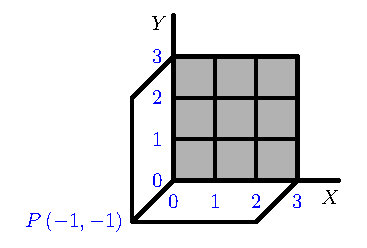
\includegraphics[height=4cm]{rubik-doc-figB.pdf}
% \else
% 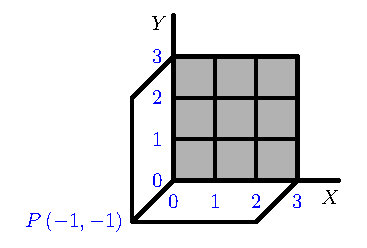
\includegraphics[height=4cm]{rubik-doc-figB.eps}
% \fi
%
% \parbox{9cm}{\caption{\label{fig:cubesquaregraph}Origin of coordinates 
%  is at the  bottom left corner of the grey \textsc{front} face. 
%  Since  $P$ is  at $(-1,-1)$ then the default height and width of the 
%  2D~cube image is 4~units.}}
% \end{figure}
%
% Arranging for $P$ to be at $(-1,-1)$, as well as using the bottom-left corner 
% of the \textsc{front} face as  the origin, is a  useful  design  
% feature which make it easy to figure-out the coordinates of any point on 
% the image plane (either on the cube or outside the cube), and hence 
% facilitates the use of  TikZ commands  
% (e.g.,~\cmd{\draw} and \cmd{\node} commands) to  superimpose lines, 
% arrows and text etc.,~onto the Rubik cube (see Section~\ref{sec:arrows}).
%
%
%      \subsection[Size of cube minipage]{Size of cube \cmd{\minipage}}
%      \label{sec:sizeofminipage}
%
%  Since the the default height and width of the oblique 2D~cube image is 
% 4~units (see Section~\ref{sec:coordinates} above), 
%  it follows that the width of the \cmd{\minipage} required for a cube in a 
%  \texttt{tikzpicture}  environment can be easily calculated. For~example, 
%  if the \texttt{tikzpicture} scale factor used is $0.5$, then the minimum
%  width of the required minipage for the \cmd{\DrawRubikCubeLD} view (shown above)
%  is therefore $0.5 \times 4\mbox{cm} =  2\mbox{cm}$. 
%
% Note that the width of the semi-flat (SF) cube representation is therefore 
% 10~units ($=3+3+1+3$),  and that of the  flat (F) cube is 12~units ($=3+3+3+3$)
%  --- see Section~\ref{sec:flatcommands} for images of these forms. 
% If in doubt check the  horizontal extent of an image  using the \cmd{\ShowCubeF} command,
% which places an fbox around the image.
%
%
%
%    \section{TikZ picture environment}
%      \label{sec:tikz}
% 
%  All the Rubik bundle \cmd{\Draw..} commands are designed to be used 
% with the TikZ picture environment, and  are compatible with standard TikZ. 
%  For a basic introduction to the use of TikZ see the following manuals
%  (from CTAN or from \texttt{http://altermundus.com/}).
%  \begin{itemize}
%  \item \texttt{https://en.wikipedia.org/wiki/PGF/TikZ}
%  \item \texttt{pgfmanual.pdf}, version 3.0.1a (2015) (1161 pages)
%  \item \texttt{pgfplot.pdf}, version 1.14 (2016) (561 pages)
%  \item \texttt{tkz-base-screen.pdf}, version 1.16c (2011) (91 pages)
%  \end{itemize}
% An example of the TikZ picture environment for use with the Rubik bundle 
% is as follows:  
% \begin{quote}
%\begin{verbatim}
% \begin{tikzpicture}[scale=0.5]
% ...
% \end{tikzpicture}%
%\end{verbatim}
% \end{quote}
% If no scale-factor is used (default scale-factor = 1), then each of the small
% cubie sides  will have a length of 1~cm.
%
% \textsc{useful commands}:\  Probably the most  
% useful TikZ commands for use with regard 
% to the Rubik bundle are the \cmd{\draw} command (for drawing  lines, arrows, circles), 
% and the \cmd{\node} command (for writing text at specific coordinate locations). 
% The basic structure of these commands  is as~follows, where 
% (x,y) represent grid coordinates of start or end points of lines or arrows, 
% or of a circle centre, or of text position 
% (see Sections~\ref{sec:drawrubikcubecommands} and \ref{sec:arrows} for examples).
% \begin{quote}
% \begin{verbatim}
% \draw[->,thick,color=blue] (4.5, 2.5) -- (3.5,2.5);
% \draw[->,ultra thick,color=red] (4.5, 2.5) -- (3.5,2.5);
% \draw [color=blue, thick] (0.3, 0.3)  circle (1.3);
% \node (B) at (7.5, 1.5)   [black]{\small\textsf{B}};
%\end{verbatim}
%\end{quote}
% Remember that all TikZ commands  which are valid inside a \texttt{tikzpicture}
% environment require a terminal semicolon (see Section~\ref{sec:arrows} 
% for examples).
%
% \textsc{colours}: \ 
% The following colors are predefined by TikZ: red, green, blue, cyan, magenta, 
% yellow, black, gray, darkgray, lightgray, brown, lime, olive, orange, pink, 
% purple, teal, violet and white (see \texttt{https://en.wikipedia.org/wiki/PGF/TikZ}).
%
% \textsc{line width}: \
%  TikZ allows line width to be specified directly 
% (e.g.,~\texttt{[line width=<dimension>]}), or by using the following abbreviations: 
%  `ultra thin' for 0.1pt,  `very thin' for 0.2pt, `thin' for 0.4pt (the default width), 
% `semi thick' for 0.6pt, `thick' for 0.8pt, `very thick' for 1.2pt, 
% `ultra thick' for 1.6pt (see \texttt{https://en.wikipedia.org/wiki/PGF/TikZ}).
%
%% \textsc{white space}: \ 
% A particularly useful feature of  TikZ  is that it automatically 
% minimises any horizontal white-space. However, it is good practice to place 
% a \% symbol after the \verb!\end{tikzpicture}! command  
% to avoid  additional white space inadvertently being added by \LaTeX\
%  (see Section~\ref{sec:trailingpercent}).
%
% When making images it can be helpful to place them inside a  minipage 
% (e.g.,~using the  \cmd{\ShowCube}  command / environment below).
% A~convenient approach is to  first adjust  the  value of the  tikzpicture scale-factor
%  (to obtain the appropriate size), and  then adjust the minipage-width as necessary, using
% the fbox associated with the \cmd{\ShowCubeF} command  
% (see Section~\ref{sec:sizeofminipage} for a useful guide on this).
%
%  The main `display' tool for  drawing cubes is the \cmd{\ShowCube} command 
% (see below), and this  incorporates a 
% TikZ picture environment inside a minipage. The equivalent tool for 
% displaying rotation sequences is the \cmd{\ShowSequence} command.
% 
%
%
%
%
%   \section[ShowCube command]{\cmd{\ShowCube} command}
%   \label{sec:showcube}
%
%
% \DescribeMacro{\ShowCube}
% This command  \cmd{\ShowCube}\marg{width}\marg{scale-factor}\marg{commands}
% is a convenient tool  for placing  one  or more commands  inside a 
% tikzpicture environment  which is also inside a minipage
% (see Section~\ref{sec:showcubecode} for the code).
% This command takes three arguments: the first (\verb!#1!) is the  minipage width, 
% the second (\verb!#2!) is  the tikzpicture scale  factor, and the third (\verb!#3!) 
% is a  series of any \rubikcube\ package  \cmd{\Draw..}  and other commands, as well as 
% any TikZ commands which are valid in  a \texttt{tikzpicture} environment 
% (e.g.,~\cmd{\draw} or \cmd{\node}  etc.). 
% 
% \medskip
% 
% \noindent\textsc{usage}:
% The following \cmd{\ShowCube} command  displays a Rubik cube 
% (the `SixT's configuration\footnote{The \cmd{\sixts} macro is from the \textsc{rubikpatterns}
% package.})  and a blue arrow  in a  minipage of  width~3cm,  using a tikzpicture scale 
% factor of~0.5.
% Note that the  TikZ  \cmd{\draw} command requires a terminal 
% semicolon (see Section~\ref{sec:tikz}).
% 
% \medskip
%
% {\noindent}%
% \begin{minipage}{6.6cm}
%\begin{verbatim}
% \RubikCubeSolved
% \RubikRotation{\sixts}
% \ShowCube{3cm}{0.5}{%
%     \DrawRubikCubeLU
%     \draw[->,thick,color=blue] (4.5, 2.5) -- (3.5,2.5);
%      }
%\end{verbatim}
% \end{minipage}
% \hspace{2.5cm}%
%\RubikFaceUp{Y}{Y}{W}{W}{W}{W}{Y}{Y}{W}%
%\RubikFaceDown{Y}{W}{W}{Y}{Y}{Y}{Y}{W}{W}%
%\RubikFaceLeft{B}{G}{G}{B}{B}{B}{B}{G}{G}%
%\RubikFaceRight{G}{B}{B}{G}{G}{G}{G}{B}{B}%
%\RubikFaceFront{O}{O}{O}{R}{O}{R}{R}{O}{R}%
%\RubikFaceBack{O}{R}{O}{O}{R}{O}{R}{R}{R}%
% \ShowCube{3cm}{0.5}{%
%     \DrawRubikCubeLU
%     \draw[->,thick,color=blue] (4.5, 2.5) -- (3.5,2.5);
%      }
%
% \medskip
%
% {\noindent}The action of the \cmd{\ShowCube} command  is illustrated below; the 
%  \cmd{\ShowCube} command on the left is equivalent to the bunch of commands
%  on the right (see Section~\ref{sec:showcubecode} for the  complete code).
% $$
%  \left.  
%    \begin{array}{l}
%    {\ }\\
%    {\ }\\
%    \verb!\ShowCube{3cm}{0.5}{...}!\\
%    {\ }\\
%    {\ }\\
%    \end{array}
%   \right\{       
%          \begin{array}{l} 
%          \verb!\begin{minipage}{3cm}%!\\
%          \verb!\centering%!\\
%          \verb!\begin{tikzpicture}[scale=0.5]!\\
%          ...\\
%          \verb!\end{tikzpicture}%!\\
%          \verb!\end{minipage}%!\\
%          \end{array}
% $$
%
% \DescribeMacro{\ShowCubeF}
% The  \cmd{\ShowCubeF} command is similar in all respects except that it places 
% an \texttt{fbox} around the minipage in order to enable users to see the extent of any 
% associated white space. For~example, unexpected spacing between two adjacent images, 
% or between an  image and adjacent text, is usually related to 
% `hidden' white-space associated with the image itself or excessive width 
% of the associated \cmd{\minipage} (see also Section~\ref{sec:trailingpercent}).
% Consequently,  a temporary \texttt{fbox} around the minipage can be a 
% useful aid  when trying to  visualise the  full extent of the minipage 
% (and its associated white-space). Use the \cmd{\ShowCubeF} command for this. 

% For~example, the following use of the \cmd{\ShowCubeF} command reveals a significant 
% white-space problem:
%
% \medskip
%{\noindent}%
%\begin{minipage}{6.6cm}
%\begin{verbatim}
% \ShowCubeF{4cm}{0.3}{\DrawRubikCubeRU}
%\end{verbatim}
%\end{minipage}
% \RubikCubeSolved
% \ShowCubeF{4cm}{0.3}{\DrawRubikCubeRU}
%
% \medskip
% {\noindent}In this example, clearly either the minipage is too wide (4cm) 
% or the \texttt{tikzpicture} scale factor is too  small (0.3). 
% Once the figure/code has been corrected, then the 
% \texttt{F}  in  the  \cmd{\ShowCubeF} command  can be removed. 
%
% Note that while the \cmd{\ShowCube} command centres  the image  
% inside the minipage, \LaTeX\ positions 
% the minipage in the \cmd{\textwidth}, and  hence it is  generally best to minimise 
% the horizontal white-space as revealed by the \cmd{\ShowCubeF}  command.  The~relationship 
% between the required width of the minipage and the TikZ  scale factor  for the various 
% Rubik cube images is detailed in  Section~\ref{sec:sizeofminipage}.
%
%
%
%     \section{Optimum strategy}
%     \label{sec:optimumstrategy}
%
%  
% We suggest that the  most convenient (and intuitive) approach for drawing 
% cubes or  particular faces is to do it in stages, as follows 
% (all these steps are well illustrated  in the examples file 
% \texttt{RubikExamples.pdf}):
%\begin{itemize}
% \item first, start by setting the  colour state of the cube. This can be done using 
% either (a)~a \cmd{\RubikCubeSolved..}  or \cmd{\RubikCubeGrey..} command 
% (for defining the whole cube),  or (b)~using one or more \cmd{\RubikFace..}  
% commands (for defining parts of faces),  or (c)~by imputting  a file containing  
% a previously saved colour state\footnote{See the \textsc{rubikrotation} package documentation 
% for details of the \cmd{\SaveRubikState} command; see also the `SaveRubikState' example  in the 
% file \texttt{RubikExamples.pdf}.}.
%
% \item second,  use the \cmd{\RubikRotation}\ command to process a sequence of rotations 
% (remembering that this requires use of the \verb!--shell-escape! command-line option).
% The \textsc{rubikpatterns} package is a small library of named rotation sequences.
%
% \item third, draw  the image(s) using  \cmd{\DrawRubikCube..} or
%  \cmd{\DrawRubikFace..} commands, plus any TikZ commands 
% (e.g.,~\cmd{\draw} and/or \cmd{\node}) in conjunction with the \cmd{\ShowCube} command. 
% Use the \cmd{\ShowCube} scale factor to adjust the size, and use the \cmd{\ShowCubeF}
% command to reveal the extent of any \texttt{minipage} whitespace. 
%
% \item fourth, spacing between graphic elements can be influenced by adjusting either 
% (a)~horizontal whitespace as set by the \cmd{\ShowCube} command, or (b)~using standard
%  \TeX\ spacing commands, e.g.,~\cmd{\quad}, \cmd{\qquad}, \cmd{\hspace..} etc.
%
% \item finally, give some thought to using a trailing \verb!%! in commands which are 
% broken across multiple lines (see Section~\ref{sec:trailingpercent}).
%
%\end{itemize}
% With this approach  the internal colour state 
%  will be updated and  processed correctly by all subsequent 
% \cmd{\Draw..} or \cmd{\RubikRotation}\ commands. 
% Note that exchanging the word `\texttt{Rubik}' for the word `\texttt{Two}' in a command will  
% generate the equivalent TwoCube version of the command (see Section~\ref{sec:rubikandtwo}).
% 
%
%
%    \section{Colour commands}
%      \label{sec:colours}
%
% The Rubik bundle of packages  uses seven colours which are defined as follows: 
% R~(red), O~(orange), Y~(yellow),  G~(green), B~(blue),  W~(white), 
% and   X~(grey). Now  according to the following webpage\,\footnote{We thank Peter Bartal  
% for bringing this webpage to our attention.} 
%
% \medskip
% \noindent\texttt{http://The-Rubiks-Cube.deviantart.com/journal/Using-Official-Rubik}
% \newline\texttt{-s-Cube-Colors-268760351} (Nov 2011)
%
% \medskip
% {\noindent}the official Rubik cube colours are defined as
% \begin{quote}
%\begin{verbatim}
% ... colours which are red (PMS 200C*), green (PMS 347C*),
% blue (PMS 293C*), orange (PMS 021C*), yellow (PMS 012C*)
% and white.
% ...
% Pantone colors can not be accurately converted to RGB colors, 
% the colors the web runs on. But they can be approximated. 
% Through some research, I have found some estimations which 
% may help you which I have listed below. Remember, these are
% just approximate RGB equivalents to the official Rubik's Cube
%  colors.
% 
% Red: 200C #C41E3A  (www.perbang.dk/rgb/c41e3a/)
% Green: 347C #009E60 (www.perbang.dk/rgb/009e60/)
% Blue: 293C #0051BA (www.perbang.dk/rgb/0051ba/)
% Orange: 021C "Pantone Orange" #FF5800 (www.perbang.dk/rgb/ff5800/)
% Yellow: 012C "Pantone Yellow" #FFD500 (www.perbang.dk/rgb/ffd500/)
% White: N/A #FFFFFF
%
% Red    {HTML}{C41E3A}
% green  {HTML}{009E60}
% Blue   {HTML}{0051BA}
% Yellow {HTML}{FFD500}
% Orange {HTML}{FF5800}
% White  {HTML}{FFFFFF}
%\end{verbatim}
% \end{quote}
%
% {\noindent}The following RGB specifications  are given by Sher (2014):
% \begin{quote}
%\begin{verbatim}
% White  {RGB}{255,255,255}
% Red    {RGB}{137,18,20}
% Blue   {RGB}{13,72,172}
% Orange {RGB}{255,85,37}
% Green  {RGB}{25,155,76}
% Yellow {RGB}{254,213,47}
%\end{verbatim}
% \end{quote}
%
%  {\noindent}However, we have tried to optimise these prescribed colours very slightly 
%  for screen \& print use (for~example, the yellow  was made very 
%  slightly brighter),  and so the actual colours implemented by 
%  the \rubikcube\ package  are as follows\,\footnote{Although the Pantone
%  colours cannot be converted to RGB, there is a subset of of Pantone colours
%  which can be be converted using CMYK 
%  (see \texttt{https://en.wikipedia.org/wiki/Pantone}).}
%  (see Section~\ref{sec:codecolours}):
%
% \begin{quote}
%\begin{verbatim}
% \definecolor{R}{HTML}{C41E33}
% \definecolor{G}{HTML}{00BE38}
% \definecolor{B}{HTML}{0051BA}
% \definecolor{Y}{HTML}{FFFF00}
% \colorlet{O}{orange}
% \colorlet{W}{white}
% \colorlet{X}{black!30}%
%\end{verbatim}
% \end{quote}
% Different colours  can be allocated   to  the ROYGBWX letters  (using the 
% standard \LaTeX\ \cmd{\colorlet} command) as required. For~example, the 
% standard `red'  colour could  be allocated to the letter R using the command
% \begin{quote}
%    \cmd{\colorlet\{R\}\{red\}}
% \end{quote}
% However, it is important to appreciate that  the letter codes 
% ROYGBWX are `hardwired' into many of the macros in the \rubikcube\ package,
%  so don't change these.
%
%
%
%     \subsection{Colour state of the cube}
%     \label{sec:colourstate}
%
% A given cubie facelet on a given face is denoted using an ordered sequence 
% of three letters, as follows:  first the face code (U,D,L,R,F,B), 
% second the X-position of the column (l,m,r), 
% and third the Y-position of the row (t,m,b). 
% For example, the `right-bottom' facelet of the  \textsc{front} face is denoted as
% \texttt{Frb}, and consequently the curent colour-code (R,O,Y,G,B,W,X) of this  facelet 
% is held as the variable \cmd{\Frb} etc.\ 
% (see Section~\ref{sec:rubikfacecode} for details and  code).
%
%
% Initially, when \LaTeX\ reads the file \texttt{rubikcube.sty} all facelets
% are allocated the colour-code X, which can be regarded as a zero-colour state. 
% Until a facelet is allocated  one of the six  cube  colours (using a suitable command)
% it will be  rendered as  grey by a  \cmd{\Draw...} command, since these commands 
%  simply implement the current  colour state of the cube (e.g.,~\cmd{\DrawRubikCubeRU}).
% Facelets  retain their colour allocation even if they are moved using  
% the \cmd{\RubikRotation} command (see \textsc{rubikrotation} package), unless they are 
% overwritten by a subsequent colour allocation command.
%
%  \DescribeMacro{\RubikFace..}
%  \DescribeMacro{\RubikSlice..}
%  \DescribeMacro{\RubikCubeSolved..}
%  \DescribeMacro{\RubikCubeGrey..}
%  \DescribeMacro{\RubikCubeGreyAll}
% Colours are allocated  to facelets using using \cmd{\Rubik..} commands.
% For example,  the commands \cmd{\RubikCubeSolvedWY} and \cmd{\RubikCubeSolvedWB} 
% allocate   prescribed  colour states for the whole `solved' cube, and are 
% a very useful starting   point (configuration) for subsequent rotations.
% The commands \cmd{\RubikCubeGreyWY} and  \cmd{\RubikCubeGreyAll}   allocate  different colour 
% states for the whole cube, and are designed to be useful starting points when illustrating
% aspects of how to solve the cube. These two commands accept both `grey' and `gray' 
% (to be consistent with TikZ).
%
% Colours can also be allocated to subsets of facelets (eg faces, slices etc); 
% for  example, using the 
% commands   \cmd{\RubikFace...} and \cmd{\RubikSlice...} 
% commands (see Sections~\ref{sec:rubikfacecommands} and \ref{sec:slicecommands}).  
%
% To  visualise the current state of the cube one has to use a  \cmd{\Draw...} command.
% \cmd{\Draw..} commands  never influence the internal  colour state of the 
% cube.\footnote{That said, the now deprecated \cmd{\DrawRubikLayerFace...} 
% and \cmd{\DrawRubikLayerSice...} commands 
% (see Section~\ref{sec:deprecated}) did, confusingly, allow you  to specify colours 
%  as arguments, but they only `painted' colours onto  facelet positions  
% (on the page, so to speak), and for this reason they are now deprecated, 
%  and will be phased out in due course.} 
%
% The current colour state / configuration of a  cube can also be saved and 
%  written to a named file, which can then be  \cmd{\input} and processed later when required,
%  using the  \cmd{\SaveRubikState} command (3x3x3 cube)
% or \cmd{\SaveTwoState} command (2x2x2 cube).
%
%
%
%  \subsection{RubikFace commands}
%   \label{sec:rubikfacecommands}
%
%  \DescribeMacro{\RubikFaceUp}
%  \DescribeMacro{\RubikFaceDown}
%  \DescribeMacro{\RubikFaceLeft}
%  \DescribeMacro{\RubikFaceRight}
%  \DescribeMacro{\RubikFaceFront}
%  \DescribeMacro{\RubikFaceBack}
% These  commands  allocate   colours to the 
% individual cubies  of a 3x3x3 cube face; they take nine colour arguments 
% (see Section~\ref{sec:rubikfacecode} for the code).
% The ordering is isomorphic to the sequence 1--9, i.e.,~numbering the small 
% squares 1-3~(top row, left to right), 4-6~(middle row, left to right), 
% 7-9~(bottom row, left to right), as follows:
% \begin{quote}
% \fbox{
% \begin{minipage}{1.6cm}
% \#1 \#2 \#3 
%
% \#4 \#5 \#6
%
% \#7 \#8 \#9
% \end{minipage}
% }
% \end{quote}
% Conveniently, \LaTeX\ allows the colour arguments to be separated by spaces 
% (e.g.,~in groups of three), or even spread across several 
% lines (e.g.,~in a square block to resemble a 9-face). This is fortunate, as it
%  allows the command to be written in several visually intuitive ways, as follows:
%
% \begin{quote}
% \begin{minipage}{8cm}
%\begin{verbatim}
% \RubikFaceUp{G}{B}{G}   {G}{W}{O}   {G}{O}{G}
%
% \RubikFaceFront{O}{W}{R}
%                {W}{W}{W}
%                {G}{W}{G}
% 
%\end{verbatim}
% \end{minipage}
% \end{quote}
% Failure to include a valid colour argument  will generate a 
% `missing parameter' error, and no colour will be 
% allocated (i.e.,~you will see  a black-hole) when it is rendered.
%
%  \DescribeMacro{\RubikFaceUpAll}
%  \DescribeMacro{\RubikFaceDownAll}
%  \DescribeMacro{\RubikFaceLeftAll}
%  \DescribeMacro{\RubikFaceRightAll}
%  \DescribeMacro{\RubikFaceFrontAll}
%  \DescribeMacro{\RubikFaceBackAll}
% Each of the above commands has an associated 
% `\texttt{All}' version which allocates  the same colour to all the cubies 
% on a 9-face  (i.e.,~only a single colour argument is required).
% For example, if you want the \textsc{right} face to be all orange, then 
%  use  the command \cmd{\RubikFaceRightAll\{O\}}.
% Use of these commands is shown in the following example.
%
%
% \bigskip
% 
% \begin{minipage}{2.8cm}
% \RubikCubeGreyAll
% \RubikFaceRightAll{O}
% \RubikFaceFront{W}{Y}{G}
%                {W}{Y}{G}
%                {W}{Y}{G}
% \begin{tikzpicture}[scale=0.7]
% \DrawRubikCubeRU
% \end{tikzpicture}%
% \end{minipage}
%    \hspace{5mm}
% \begin{minipage}{0.6\textwidth}
%\begin{verbatim}
% \RubikCubeGreyAll
% \RubikFaceRightAll{O}
% \RubikFaceFront{W}{Y}{G}
%                {W}{Y}{G}
%                {W}{Y}{G}
% \ShowCube{3cm}{0.7}{\DrawRubikCubeRU}
% \end{verbatim}
% \end{minipage}
%
% \bigskip
%
%
% Note that instead of using  \cmd{\RubikCubeGreyAll}  we could have used the 
% command \verb!\RubikFaceUpAll{X}! to allocate grey to the whole of the 
%  \textsc{up} face. However, the  \cmd{\RubikCubeGreyAll} command can be  a useful 
% starting point when dealing with a new cube,  
% since it resets all the faces to their initial default colour.
%
% Finally, it is important to bear in mind that when allocating colours using 
% the \cmd{\RubikFace..} commands  it is very 
% easy to inadvertently create a non-valid cube (ie a cube with either the wrong number
% of facelets with particular colours, or one which has a non-sovable configuration).
% However, some basic error checking of this sort is done whenever the 
% \cmd{\RubikRotation} command is used
% (see the \textsc{rubikrotation} package documentation).

%
%
%       \subsection{RubikSolvedConfig command}
%       \label{sec:rubiksolvedconfig}
%
%  \DescribeMacro{\RubikSolvedConfig}
% This command  allocates  the six face colours according to the following ordered 
% XYZ$+-$  argument rule, namely X$+$, X$-$, Y$+$, Y$-$, Z$+$, Z$-$; i.e.,~the order 
% of the six colour arguments follows the face order
% \textsc{right, left, up, down, front, back} (for notation see  
% Section~\ref{sec:xyzarguments}  and Figure~\ref{fig:notation}). 
% {\newline}\textsc{usage}:\ \verb!\RubikSolvedConfig{G}{B}{W}{Y}{O}{R}!
% {\newline}Examples of its use are shown in the  next section.
%
%
%
%
%       \subsection{RubikCubeSolved commands}
%       \label{sec:rubikcubesolved}
%
%  \DescribeMacro{\RubikCubeSolved}
%  \DescribeMacro{\RubikCubeSolvedWY}
% The action of both of these  commands is identical: 
% they both  set all the face colours to the following  standard `solved' cube
% configuration, namely  Up=white, Down=yellow, Right=green, Left=blue, Front=orange, Back=red,
% by invoking the above \cmd{\RubikSolvedConfig} command,  as follows:
%\begin{verbatim}
%\newcommand{\RubikCubeSolved}{\RubikSolvedConfig{G}{B}{W}{Y}{O}{R}}
%\end{verbatim}
% Note that this is in fact just a convenient short-hand for the following:
%\begin{verbatim}
%\newcommand{\RubikCubeSolved}{%
%  \RubikFaceRightAll{G}%
%  \RubikFaceLeftAll{B}%
%  \RubikFaceUpAll{W}%
%  \RubikFaceDownAll{Y}%
%  \RubikFaceFrontAll{O}%
%  \RubikFaceBackAll{R}%
%}
%\end{verbatim}
% Note that for convenience, this configuration is also available using the command
% \verb!\RubikCubeSolvedWY! (WY denoting White opposite Yellow).
% This solved configuration is shown in the following 
% semi-flat (SF) image.
%
%
% \bigskip
%
% \begin{minipage}{5cm}
% \centering
% \begin{tikzpicture}[scale=0.5]
% \RubikCubeSolvedWY
% \DrawRubikCubeSF
% \end{tikzpicture}%
% \end{minipage}
% \begin{minipage}{0.5\textwidth}
%\begin{verbatim}
%  \RubikCubeSolvedWY
%  \ShowCube{5cm}{0.5}{\DrawRubikCubeSF}
%\end{verbatim}
% \end{minipage}
%
% \bigskip
%
% Note that the width of the minipage  used in the  \cmd{\ShowCube} command above  
% is set to 5cm. This value is derived from the fact 
% that  the \textit{unscaled} width of the semi-flat image is 10cm (9 + 1 squares), and hence if
% the TikZ scale factor is set to 0.5 (as in the above example) then the minimum minipage 
% width = $10 \times 0.5 = 5$cm (see Section~\ref{sec:coordinates} for details).
%
%
% \textbf{Other orientations:} If other orientations of the solved cube are required, 
% this can be easily achieved using the \cmd{\RubikRotation} command 
% (from the \texttt{RubikRotation} package) to rotate the cube as required.
% For~example, we could make a command to show the above solved cube upside-down 
% and rotated slightly, as follows:
%\begin{verbatim}
%\newcommand{\CubeUpSideDown}{\RubikCubeSolved\RubikRotation{x2,y}}
%\end{verbatim}
% ---this uses  the rotations \rrx, \rrx, to invert, and then  \rry\ to turn 
% the cube 90~$\deg$:
%
% \bigskip
%
% \begin{minipage}{2.6cm}
% \centering
% \begin{tikzpicture}[scale=0.5]
% \DrawNCubeAll{3}{O}{Y}{G}
% \end{tikzpicture}%
% \end{minipage}
%    \hspace{5mm}
% \begin{minipage}{0.6\textwidth}
%\begin{verbatim}
% \CubeUpSideDown
% \ShowCube{2cm}{0.5}\DrawRubikCubeRU}
%\end{verbatim}
% \end{minipage}
%
% \bigskip
%
%%  \DescribeMacro{\RubikCubeSolvedWB}
%  \textbf{Other configurations:} While the `solved' WY colour configuration 
% described above (White face opposite Yellow) 
% is that of the most commonly occurring  Rubik cube, another  `solved' colour configuration
% which is also commercially available has the White opposite Blue configuration, which 
% is available  using the command \verb!\RubikCubeSolvedWB!.
% Its  colour configuration is as follows:
%
%\begin{center}
% \RubikCubeSolvedWB
% \ShowCube{4cm}{0.4}{\DrawRubikCubeSF}%
%\end{center}
%
% \bigskip
%
% Note that  users can easily create their own alternative `solved'  
% face/colour versions.
% For~example, the above mentioned  white opposite
% blue~(WB)  solved configuration  command \verb!\RubikCubeSolvedWB!  
% (white opposite blue, red opposite orange, 
% and green opposite yellow), was created using  \verb!\RubikSolvedConfig{R}{O}{W}{B}{G}{Y}!
% (for the code see \ref{sec:codesolvedconfig}).
%
%
%
%
%       \subsection{RubikCubeGrey.. commands}
%       \label{sec:rubikcubegrey}
%
%  \DescribeMacro{\RubikCubeGreyWY}
%  \DescribeMacro{\RubikCubeGreyWB}
%  \DescribeMacro{\RubikCubeGreyAll}
%  The command \cmd{\RubikCubeGreyWY} generates a 3x3x3 cube with no colours allocated 
%  \textit{except} for the central  cubie of each face, which takes the same colour 
%  configuration as defined for the  \cmd{\RubikCubeSolvedWY} command. 
%  The command \cmd{\RubikCubeGreyAll} generates a cube with \textit{all} the faces 
%  completely grey; this is useful as it can be used to reset all the facelets to 
%  the initial default  state.
%  These commands will accept either `grey' or  `gray' (to be consistent with TikZ).
%
%  These  commands, are designed to be  useful starting points when wanting to 
%  describe the movement of particular cubies. We can see  the effect of 
%  the \cmd{\RubikCubeGreyWY} command by viewing the cube in a semi-flat (SF) format, 
%  as follows:
%
% \bigskip
%
% \RubikCubeGreyWY
% \ShowCube{4.5cm}{0.45}{\DrawRubikCubeSF}
%    \hspace{3mm}
% \begin{minipage}{0.6\textwidth}
%\begin{verbatim}
% \RubikCubeGreyWY
% \ShowCube{4.5cm}{0.45}{\DrawRubikCubeSF}
%\end{verbatim}
% \end{minipage}
%
% \bigskip
%  Users can of course  set up their own alternative  face/colour configuration 
% by  creating a new `variant'  command  altogether. 
%
%
%
%    \subsection{RubikSlice commands}
%   \label{sec:slicecommands}
%
%  \DescribeMacro{\RubikSliceTopX}
%  \DescribeMacro{\RubikSliceMiddleX}
%  \DescribeMacro{\RubikSliceBottomX}
%  These three commands  allocate the six visible cubie colours associated with  a
%   \textit{horizontal}  slice of a Rubik cube. 
% There are three pairs of  Slice commands; one pair 
% (Left view \& Right view) for each of the horizontal  slices Top, Middle, Bottom.
% The six colour arguments  associated with a given slice run in sequence 
% from left to right irrespective of the viewpoint, e.g.,~\#1 \#2 \#3   \#4 \#5 \#6.
%
% Since the viewpoint of the Rubik cube (from the Right or from the Left) 
% influences which face the colours are associated with, it is necessary 
% to have the view (R or L) specified in the command name.
%
% The format of the `slice' command is shown in the following example.
% The Rubik  cube is shown from  the LeftDown (LD) view 
% and consequently  each of the `slice' commands in this
% particular example  ends in L, consistent with 
% the final \cmd{\DrawRubikCubeLD} command.
%
% Note that the two legacy `Equator' versions (now replaced by `Middle') 
% are retained to allow backward compatibility. 
%
% \bigskip
%
% \begin{minipage}{2.8cm}
% \centering
% \RubikFaceDownAll{Y}
% \RubikSliceTopL    {G}{G}{G} {R}{R}{R}
% \RubikSliceMiddleL {R}{R}{R} {B}{B}{B}
% \RubikSliceBottomL {O}{O}{O} {G}{G}{G}
% \begin{tikzpicture}[scale=0.7]
% \DrawRubikCubeLD
% \end{tikzpicture}%
% \end{minipage}
%    \hspace{5mm}
% \begin{minipage}{0.6\textwidth}
%\begin{verbatim}
%    \RubikFaceDownAll{Y}
%    \RubikSliceTopL     {G}{G}{G} {R}{R}{R}
%    \RubikSliceMiddleL  {R}{R}{R} {B}{B}{B}
%    \RubikSliceBottomL  {O}{O}{O} {G}{G}{G}
%    \ShowCube{3cm}{0.7}{\DrawRubikCubeLD}
%\end{verbatim}
% \end{minipage}
%
%
%
%
%
%      \section{Rotation commands}
%      \label{sec:RubikCommands} 
%
% The Rubik bundle implements not only the standard Rubik cube notation  of the 
% World Cube Association (see WCA website), but also the main variant notations 
% used by the  Rubik interest groups and websites.  
%
% \begin{figure}[hbt]
%  \centering
%  \ifpdf
%    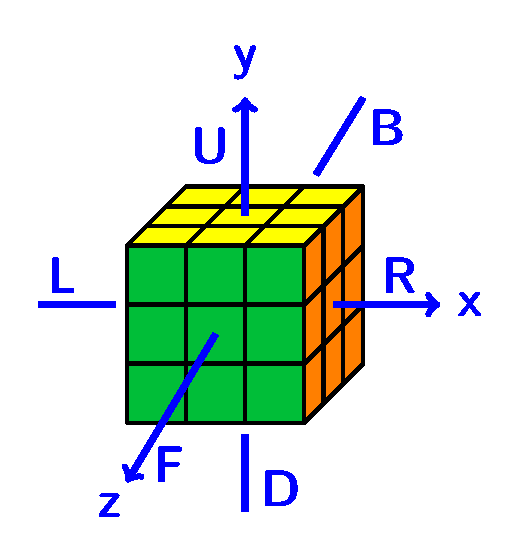
\includegraphics[height=5cm]{rubik-doc-figA.pdf}
%  \fi
% \caption{\label{fig:notation}Face rotations} 
% \end{figure}
%
% To avoid confusion the Rubik bundle uses a trailing `p' (lower case) in rotation-codes to denote 
% a `prime' (reversed direction); we also recommend that  commas  are used to separate 
% sequential Rubik rotations (moves). 
% While these are mainly to avoid  ambiguity,  they also greatly facilitate computer 
% searching  and  copy-and-pasting  of rotation sequences.
%
%  Unfortunately, obtaining a good balance between an intuitive notation for defining
%  rotations and the need for flexibility is difficult,
% and consequently some notation is more intuitive than others. A good compromise 
% seems to be the World Cube Association's FADN structure; i.e.,~Face (L,R,U,D,F,B), 
% Action (m,w,s,a,c), Direction (p), 
% N (n); for~example, codes like \texttt{R, R2, Rc, Rm, Rwp, Rwp2} etc.  
%
%
% The \rubikcube\  package  includes  commands for typesetting a wide range of 
% rotation-codes (e.g.,~\rr{R}, \rr{y}, \rr{Bw}) and 
% equivalent  hieroglyphs  (e.g.,~\rrh{R}, \rrh{y}, \rrh{Bw}), as well as commands
% for typesetting  3x3x3 cubes\,\footnote{See the \textsc{rubiktwocube} package documentation 
% for 2x2x2 cube commands.} and single cubies. All the rotation-codes and 
% hieroglyphs are typeset using  one particular font \& size which we call the `rubikfont'
% for convenience (see Section~\ref{sec:rubikfont} for details).
% All of the rotation-codes described
% here are recognised by the \textsc{rubikrotation} package 
% (see Section~\ref{sec:rubikrotation}).
%
% Note that there are some rotation codes which  are not represented by arrow 
% hieroglyphs, since their rotation  is not visible from the \textsc{front} face, 
% and hence cannot easily be rendered as  an arrow hieroglyph. Consequently these 
% rotations  have a simple `letter' hieroglyph 
% in the form of the rotation-code in a square; for~example, \rrhBw, \rrhFm. 
%
%
%
%   \subsection{Typesetting}
%     \label{sec:typesetting}
%
% We now describe the four commands used for typesetting the various rotation-codes. 
%
% \DescribeMacro{\rr}
%  The text version of a  rotation-code  is typeset  using the rubik-rotation 
%  command \cmd{\rr\marg{rotation-code}}, i.e.,~\rr{R}\ is typeset using the command \cmd{\rr\{R\}}. 
% The hieroglyph of a rotation is generated  (in text) by  \DescribeMacro{\rrh}
% using instead the command \cmd{\rrh\marg{rotation-code}}. For~example, the command 
% \cmd{\rrh\{R\}} generates  \rrh{R}\  which is the hieroglyph associated with
% the rotation  \rr{R}.
%
% \DescribeMacro{\Rubik}
% A vertically combined rotation-code  and its hieroglyph  is generated using the command 
% \cmd{\Rubik\marg{rotation-code}}. For~example, \Rubik{R}\ is generated by the command \cmd{\Rubik\{R\}}, 
% with  the square hieroglyph sitting on the baseline.
% For some hieroglyphs (e.g.,~\rrh{x}, \rrh{y}, \rrh{z}\ denoting 90~degree cube-axis rotations) 
% the only  difference between the \cmd{\rrh\{\}} and \cmd{\Rubik\{\}} form is that 
% the \cmd{\Rubik\{\}}  form is elevated  to sit on the baseline just like the other
%  \cmd{\Rubik\{\}} hieroglyphs. 
% For~example, \cmd{\rrh\{yp\}} generates \rrh{yp}, while
% \cmd{\Rubik\{yp\}} generates \Rubik{yp}.
% 
% \DescribeMacro{\textRubik}
% A horizontally combined  rotation-code and its hieroglyph (in sequence as in text) 
% is generated using  the command   \cmd{\textRubik\marg{rotation-code}}. 
% For~example,  \textRubik{R}\ is typeset using the command \cmd{\textRubik\{R\}}.
% A list of all rotation-code commands and their associated  hieroglyphs is given in
%  Section~\ref{sec:listofcommands}. 
%
%
%
% \subsection{Face rotations}
%
% \DescribeMacro{U}
% \DescribeMacro{D}
% \DescribeMacro{L}
% \DescribeMacro{R}
% \DescribeMacro{F}
% \DescribeMacro{B}
% The six main faces of the cube are denoted as \textsc{front} (towards the observer), 
% \textsc{back},  \textsc{left}, \textsc{right},  \textsc{up}, \textsc{down}.
% The upper-case initial letter  of each face-name (\rr{F}, \rr{B}, \rr{L}, \rr{R}, \rr{U}, \rr{D}) 
% denotes a clockwise 90-degree rotation of the  face as shown in  
% Figure~\ref{fig:notation}. 
% For~example, \rr{D}\ is generated by the `rubik rotation' command \cmd{\rr\{D\}}.
%
% \DescribeMacro{Up}
% \DescribeMacro{Dp}
% \DescribeMacro{Lp}
% \DescribeMacro{Rp}
% \DescribeMacro{Fp}
% \DescribeMacro{Bp}
%  An appended  prime~$^\prime$ indicates an anticlockwise rotation; e.g.,~\rr{Fp}. 
%  This is sometimes written as  \rr{F}$\boldmath{^{-1}}$. The `prime' notation is 
%  achieved by appending a lower-case `p' to the face rotation command. For~example, \rr{Rp}\ 
%  is generated by \cmd{\rr\{Rp\}}. More formally, \rr{Rp} is the `inverse' of  \rr{R}.
%
%  The superscript~$^2$, or sometimes just an ordinary~2, indicates that the rotation
%  is applied twice. For~example, \rr{R}\textbf{$^2$} or \rr{R}\textbf{2} 
%  denote  \textit{two} successive 90~degree clockwise rotations of the \textsc{right} face;
%   \rr{R}\textbf{$^3$} is equivalent to \rr{Rp} etc. 
%
%
%      \subsection{Inner-slice rotations}
%      \label{sec:slicerotations}
%
% The Rubik cube (3x3x3) has three orthogonal so-called 
% `inner' slices (middle layers, middle slices), whose +ve 
% rotation  direction follows that of a named face. For~example, the inner-slice 
% rotation  between the \textsc{right} and \textsc{left} faces  whose rotation 
% direction follows the rotation \rr{R}\ (i.e.,~its rotation is isomorphic to \rr{R}).
%  The  inner-slice rotations form a group (the Slice group), originally 
% described by John Conway (Frey and Singmaster, 1982, p~105).
%
%
% \subsubsection*{The `m' notation}
%  \label{sec:mnotation}
%
% \DescribeMacro{Um}
% \DescribeMacro{Dm}
% \DescribeMacro{Lm}
% \DescribeMacro{Rm}
% \DescribeMacro{Fm}
% \DescribeMacro{Bm}
% Here `m' stands for the `middle' slice, namely  that parallel to the  designated 
% \textsc{face}; its rotation mirrors that of the 
% \textsc{face}.   The \texttt{m}  must be in lower case. 
% Each of these  rotation-codes has a complementary `prime' version, formed 
% by appending a `p'; for~example,  \rr{Rm}  (\verb!\rr{Rm}!) is a middle layer rotation 
% \rrh{Rm} between the  \textsc{right} and \textsc{left} faces, and is in the same
% direction as \rr{R}. The code \rr{Rmp} (\verb!\rr{Rmp}!) refers to the same 
% middle slice, but rotated in  the opposite direction \rrh{Rmp}.
%
%  This notation, which was probably  invented by Singmaster, was originally used on the 
%  Cube Lovers usenet group (1981--1997). It is now much used on the 
%  Jaap Puzzles website (see Scherphius J) ---see also Section~\ref{sec:codeJaap}.
%
%
% \subsubsection*{The `M' notation} 
%  \label{sec:Mnotation}
%
% \DescribeMacro{MU}
% \DescribeMacro{MD}
% \DescribeMacro{ML}
% \DescribeMacro{MR}
% \DescribeMacro{MF}
% \DescribeMacro{MB}
% This variant of the above  `middle' slice notation (e.g.,~\texttt{MR} $\equiv$ \texttt{Rm}) 
% is part of the  `superset' notation of  Randelshofer. As before,  the rotation  
% direction follows that  of the designated   \textsc{face}. 
% Each has a complementary  `prime' version  
% formed by appending a `p'.   The \texttt{M}  must be in upper case.
%
%
% \bigskip\bigskip
%
% \subsubsection*{The MES notation}
%
% \DescribeMacro{M}
% \DescribeMacro{E}
% \DescribeMacro{S}
% \DescribeMacro{Mp}
% \DescribeMacro{Ep}
% \DescribeMacro{Sp}
% An alternative but very confusing 
% inner-slice notation (e.g.,~\texttt{Ep} $\equiv$ \texttt{Um}) which is occasionally used 
% is the so-called MES notation as used in the Waterman algorithm  
% (Treep and Waterman 1987), and the Roux method (Giles Roux).
% \begin{itemize}
% \item[\rr{M}] \ (\textsc{middle} \rrh{M}, between the \textsc{left} 
%      and \textsc{right} faces;  direction  follows  \rr{L}),
% \item[\rr{E}] \  (\textsc{equator} \rrh{E}, between the \textsc{up} and \textsc{down} 
%      faces;  direction follows \rr{D}),
%  \item[\rr{S}] \  (\textsc{standing} \rrh{S}, between the \textsc{front} and 
%      \textsc{back} faces;   direction follows \rr{F}).
% \end{itemize}
% Each of these also has an inverse (prime) version.
%
%
% \subsubsection*{The `S' notation}
%
% \DescribeMacro{Su}
% \DescribeMacro{Sd}
% \DescribeMacro{Sl}
% \DescribeMacro{Sr}
% \DescribeMacro{Sf}
% \DescribeMacro{Sb}
% In this equally confusing inner-slice notation, `S' stands for `inner-slice'; 
% the face letter must  be in lower case (e.g.,~\texttt{Sr} $\equiv$ \texttt{Rm}). 
% For~example, the inner-slice 
% rotation  between the \textsc{right} and \textsc{left} faces  whose rotation 
% direction follows the rotation \rr{R}\ is denoted 
% as \rr{Sr}, which is typeset using the command \cmd{\rr\{Sr\}}. 
% Each has an inverse  (prime)  p-form.
%
%
%     \subsection{Outer-slice rotations}
%
% \subsubsection*{The `s' (slice) notation}
%
% \DescribeMacro{Us}
% \DescribeMacro{Ds}
% \DescribeMacro{Ls}
% \DescribeMacro{Rs}
% \DescribeMacro{Fs}
% \DescribeMacro{Bs}
% This is a  `paired' form of  
% notation (two rotations at once), which can be thought of as complementing the 
% inner-slice  (middle layer) rotations. 
% Each of these `slice' commands denotes a  rotation of  two opposite faces 
% in the \textit{same}  direction.
% {\linebreak}For~example, \textRubik{Us}\ $\equiv$ \textRubik{U}\ + \textRubik{Dp};
% i.e.,~both face-rotations are in the \textit{same} direction 
% as \rr{U}. Each of these rotation-codes has a complementary `anti-slice' version (see below).
%
% This notation was originally described by 
% Singmaster (Frey and Singmaster, 1982), and is much used 
% on the `Pretty patterns' page of the Fridrich website (this 
% page also has a useful link to `notation').
%
%
% \bigskip
%
% \DescribeMacro{SU}
% \DescribeMacro{SD}
% \DescribeMacro{SL}
% \DescribeMacro{SR}
% \DescribeMacro{SF}
% \DescribeMacro{SB}
% This variant of the above `slice'  notation (e.g.,~\texttt{SU} $\equiv$ \texttt{Us})
%  is part of the  `superset'  notation of Randelshofer. As before,  the rotation  
% direction follows that of the designated 
%  \textsc{face}. Each has a complementary  `prime' version  formed by appending a `p'. 
% 
%
% \bigskip\bigskip 
%

%
% \subsubsection*{The `a' (anti-slice) notation}
%
% \DescribeMacro{Ua}
% \DescribeMacro{Da}
% \DescribeMacro{La}
% \DescribeMacro{Ra}
% \DescribeMacro{Fa}
% \DescribeMacro{Ba}
% Each of these commands denotes a  rotation of  two opposite faces 
% in \textit{opposite}  directions. 
% For~example, \textRubik{Ua}\ $\equiv$ \textRubik{U}\ + \textRubik{D}.
% This notation is much used  on the `Pretty patterns' page of the 
% Fridrich website (see the note above re: `slice notation').
%
%   \bigskip\bigskip
%
%
%      \subsection{Wide rotations}
%
% \subsubsection*{The `w' notation} 
%  \label{sec:wnotation}
%
% \DescribeMacro{Uw}
% \DescribeMacro{Dw}
% \DescribeMacro{Lw}
% \DescribeMacro{Rw}
% \DescribeMacro{Fw}
% \DescribeMacro{Bw}
% The  clockwise \textit{combined} rotation of an outer face AND its adjacent inner-slice 
% (officially known as a `double block', or `double outer slice' move) 
% is denoted by appending a  lower-case  \textbf{\textsf{\footnotesize{w}}} 
% (denoting `wide') to a rotation-code (endorsed  by the WCA).
% For~example,  a \textsc{right} double outer slice rotation \rrh{Rw} (\verb!\rrh{Rw}!) 
% is  denoted as \rr{Rw} (\verb!\rr{Rw}!).  The `prime' version is formed by 
% appending a `p' to the rotation-code. For~example,  \rr{Rwp}\  is generated by \verb!\rr{Rwp}!.
%
%
% \bigskip
%
% \subsubsection*{The `T' notation} 
%  \label{sec:Tnotation}
%
% \DescribeMacro{TU}
% \DescribeMacro{TD}
% \DescribeMacro{TL}
% \DescribeMacro{TR}
% \DescribeMacro{TF}
% \DescribeMacro{TB}
% This confusing variant of the above `w' notation (e.g.,~\texttt{TR} $\equiv$ \texttt{Rw}) is part of 
% the  `superset'  notation of Randelshofer. As before,  the rotation  direction 
% follows that of the designated \textsc{face}. Each has a complementary `prime' version  
% formed by appending a `p'. 
%
%   \bigskip\bigskip
%
%
%     \subsection{Axis rotations}
%
% \subsubsection*{The x, y, z notation} 
%  \label{sec:xyznotation}
%
% \DescribeMacro{x}
% \DescribeMacro{y}
% \DescribeMacro{z}
% Whole-cube clockwise rotations  of 90-degrees about about the orthogonal  axes centred 
% on the  \textsc{right}, \textsc{up}, \textsc{front}  faces are denoted 
% as \rr{x}, \rr{y}, \rr{z}\ (the \cmd{\rr\{\}} forms) respectively (see Figure~\ref{fig:notation}), 
% with their hieroglyphs (the \cmd{\rrh\{\}} forms) being denoted 
% as \rrh{x}, \rrh{y}, \rrh{z}\ in order to distinguish them from  square layer-rotation 
% hieroglyphs.
% Note that since \rr{x}, \rr{y}, \rr{z}\ rotations are always expressed in lower case;
%  this practice is also extended  to the commands. 
%
% For~example, an \rr{x}\textbf{2} rotation (two \rr{x}\ rotations one after 
% the other, i.e.,~\rrh{x}\ \rrh{x}) denotes rotating 
% the cube 180~degrees about its x axis so as to bring the \textsc{down} face  
% into the \textsc{up} position.
%
%  An appended  prime~$^\prime$ indicates an anticlockwise rotation; 
% for~example, \rr{xp}\ (which is generated by appending a `p' to the  
% rotation-code, i.e.,~\cmd{\rr\{xp\}}). 
%
% The \cmd{\Rubik\{\}}  forms (and their prime `p' versions) generate the same
%  hieroglyphs  as their \cmd{\rrh\{\}} versions, except that their spacing is 
%  similar to that associated with the `square box'  \cmd{\Rubik\{\}}  hieroglyphs.  
% Consequently  when typesetting  an axis command in a sequence of  `square-box' 
% \cmd{\Rubik\{\}} commands, it is better to use the \cmd{\Rubik\{\}} form rather than
% the equivalent \cmd{\rrh\{\}} form (see the examples in Section~\ref{sec:examples}).
% There are no \cmd{\textRubik\{\}} forms for the axis commands (since they are 
% not necessary).
%
%
% \subsubsection*{The u, d, l, r, f, b notation} 
%
%
% \DescribeMacro{u}
% \DescribeMacro{d}
% \DescribeMacro{l}
% \DescribeMacro{r}
% \DescribeMacro{f}
% \DescribeMacro{b}
% These are a commonly used  alternative for the \rr{x}, \rr{y}, \rr{z}\ notation 
% (and also endorsed  by the WCA), and denote a 90~degree whole-cube rotation  in the same 
% directional sense as that of the associated face rotation. 
%
% {\noindent}Thus  
% \rr{d}\ $\equiv$ \rr{up} $\equiv$ \rr{yp} etc.
% For~example, \rr{d}\ and \rr{dp}\ are generated by  the commands \cmd{\rr\{d\}} 
% and \cmd{\rr\{dp\}} respectively. 
% Note that \rr{u}~is the opposite of \rr{d}, \rr{l}~is the opposite of \rr{r}, and
% \rr{f}~is the opposite of \rr{b}, etc.
%
% As with the \rrh{x}, \rrh{y}, \rrh{z}\ forms (described above) there are also 
% equivalent \cmd{\rrh\{\}} and \cmd{\Rubik\{\}} forms. For~example, 
% \rrh{d}\ is generated by the command \cmd{\rrh\{d\}}.
%
%
% \pagebreak
%
% \subsubsection*{The `c' notation} 
%  \label{sec:cnotation}
%
% \DescribeMacro{Uc}
% \DescribeMacro{Dc}
% \DescribeMacro{Lc}
% \DescribeMacro{Rc}
% \DescribeMacro{Fc}
% \DescribeMacro{Bc}
% This slightly more intuitive notation (the `c' stands for `cube') also associates the rotation 
% direction  with that of the designated  \textsc{face} (e.g.,~\texttt{Rc} $\equiv$ \texttt{x}).
%  Each has a complementary `prime' version  formed by appending a `p'.  
% For~example, \rr{Rc} (\verb!\rr{Rc}!) is equivalent to \rr{x}; 
%  \rr{Rcp} (\verb!\rr{Rcp}!) is equivalent to \rr{xp}.  
%
%  This notation, which was probably invented by Singmaster, was originally used on the 
%  Cube Lovers usenet group (1981--1997). It is now much used on the 
%  Jaap Puzzles website (see Scherphius J) ---see also Section~\ref{sec:codeJaap}.
%
% \bigskip\bigskip
%
% \subsubsection*{The `C' notation} 
%  \label{sec:Cnotation}
%
% \DescribeMacro{CU}
% \DescribeMacro{CD}
% \DescribeMacro{CL}
% \DescribeMacro{CR}
% \DescribeMacro{CF}
% \DescribeMacro{CB}
% This variant of the whole cube rotation notation 
% (e.g.,~\texttt{CR} $\equiv$ \texttt{Rc} $\equiv$ \texttt{x}) 
% is part of the  `superset' notation of Randelshofer. As before, the rotation  
% direction follows that of the designated  \textsc{face}. Each has a complementary 
% `prime' version  formed by appending a `p'. 
%
%
% \bigskip% \bigskip
%
%  \subsection{Examples}
%  \label{sec:examples}
%  
%    {\noindent}\rr{R}\  is generated by  the  command \cmd{\rr\{R\}}
%
%    {\noindent}\rr{Fw}\  is generated by  the  command \cmd{\rr\{Fw\}}
%
%    {\noindent}\rr{L}$^2$ is generated by \cmd{\rr\{L\}}\verb!$^2$!
%
%    {\noindent}\rr{L}2 is generated by \cmd{\rr\{L\}2}
%
%    {\noindent}\rr{Rp}\ is generated by \cmd{\rr\{Rp\}}
%
%    {\noindent}\rr{Fwp}\  is generated by \cmd{\rr\{Fwp\}}
%
%    {\noindent}\rr{x}\ and \rrh{y}\ and \Rubik{zp}\ are  generated by 
%   \cmd{\rr\{x\}}  and \cmd{\rrh\{y\}} and \cmd{\Rubik\{zp\}}
%
%    {\noindent}\rr{Fc}\ and \rrh{Bc}\ are  generated by \cmd{\rr\{Fc\}} and \cmd{\rrh\{Bc\}}
%
%   {\noindent}\rr{U}\rr{U}\rr{R}\rr{R}\ is generated by
%      \cmd{\rr\{U\}}\cmd{\rr\{U\}}\cmd{\rr\{R\}}\cmd{\rr\{R\}}
%  
%  \medskip
%
%  {\noindent}\Rubik{F}\Rubik{U}\Rubik{y}\Rubik{Rp}\Rubik{Lwp}\
%  \ \  \verb!\Rubik{F}\Rubik{U}\Rubik{y}\Rubik{Rp}\Rubik{Lwp}!
%  
%  \bigskip
%  
%  {\noindent}\textRubik{F}\ \textRubik{U}\ \ \ \  
%       \verb!\textRubik{F}\ \textRubik{U}!
%  
%  \medskip
% 
% {\noindent}Commas can be important in avoiding  ambiguity; for~example,
%
% \medskip
%
% {\noindent}\rr{D},\rr{U}2,\rr{F}2,\rr{Ds}2,\rr{B},  \ \ \ \  \verb!\rr{U}2,\rr{F}2,\rr{Ds}2,\rr{B},!
%
%  \medskip
%
% {\noindent}\rrh{U}2,\,\rrh{F}2,\,\rrh{Ds}2,\, \ \ \ \  \verb!\rrh{U}2,\,\rrh{F}2,\,\rrh{Ds}2!
%
% \medskip
%
% {\noindent}Finally, if each rotation element uses the \textit{same} font or encoding, for~example
%
%  \medskip
%  
%  {\noindent}\rrh{F}\rrh{U}\rrh{y}\rrh{Rp}\rrh{Lwp} \ \ \ \
%  \verb!\rrh{F}\rrh{U}\rrh{y}\rrh{Rp}\rrh{Lwp}! 
%
% \medskip
%
% {\noindent}then typesetting  such a rotation  sequence  can be achieved more easily using the 
% \verb!\ShowSequence! command (see Section~\ref{sec:showsequence}). For~example, we can  
% typeset the last sequence much more conveniently, as follows:
%
% \medskip
%
% \verb!\ShowSequence{}{\rrh}{F,U,y,Rp,Lwp}! \ \ $\rightarrow$ \ \ \ShowSequence{}{\rrh}{F,U,y,Rp,Lwp}
%
%
%
%  \subsection{Backwards compatibility}
%   \label{sec:backwardscompat}
%
% Note that in keeping with `backwards compatibility'  all rotation commands (see below) 
% can still  be written without the usual curly braces \verb!{}!. 
% For~example,  the hieroglyph \rrhD\  (\cmd{\rrh\{D\}}) can also be generated using the command
%   \cmd{\rrhD}. 
%
%
%
%  \subsection{Listing of all rotation commands}
%   \label{sec:listofcommands}
%
%
% Note that all the commands presented here also have a \cmd{\Rubik\{\}} equivalent form which 
% typesets both the hieroglyph and its lettercode in a vertical format, 
% as shown in the `Examples' section above. These have been   omitted  here
% owing to the difficulty of including this form easily in the following table.
%
%
% Note also that some \cmd{\rrh\{\}} commands (e.g.,~the \cmd{\rrh\{B\}} command)  
% show only the lettercode in a square box, e.g.,~\rrh{B}. This is because these  rotations
%  do not have a `true' visual representation as seen from the \textsc{front} face,
% and hence can be somewhat ambiguous unless typeset with their associated 
% lettercode. 
%
%
%  \newcommand{\dnstrut}{\rule{0pt}{17pt}}
%  \newcommand{\dns}{\hspace{2mm}}
%  \newcommand{\dnsp}{\hspace{2mm}} 
%
%
%
%  \begin{supertabular}[lll]{p{3cm} p{3cm} p{4.5cm}}
%  \dnstrut\rr{U}\dns\cmd{\rr\{U\}}
%  & \rrh{U}\dns\cmd{\rrh\{U\}}
%  & \textRubik{U}\dns\cmd{\textRubik\{U\}} \nonumber\\ 
%  \dnstrut\rr{Up}\dns\cmd{\rr\{Up\}}
%  & \rrh{Up}\dns\cmd{\rrh\{Up\}}
%  & \textRubik{Up}\dns\cmd{\textRubik\{Up\}} \nonumber\\ 
%  \dnstrut\rr{Uw}\dns\cmd{\rr\{Uw\}}
%  & \rrh{Uw}\dns\cmd{\rrh\{Uw\}}
%  & \textRubik{Uw}\dns\cmd{\textRubik\{Uw\}} \nonumber\\ 
%  \dnstrut\rr{Uwp}\dns\cmd{\rr\{Uwp\}}
%  & \rrh{Uwp}\dns\cmd{\rrh\{Uwp\}}
%  & \textRubik{Uwp}\dns\cmd{\textRubik\{Uwp\}} \nonumber\\ 
%  \dnstrut\rr{Us}\dns\cmd{\rr\{Us\}}
%  & \rrh{Us}\dns\cmd{\rrh\{Us\}}
%  & \textRubik{Us}\dns\cmd{\textRubik\{Us\}} \nonumber\\ 
%  \dnstrut\rr{Usp}\dns\cmd{\rr\{Usp\}}
%  & \rrh{Usp}\dns\cmd{\rrh\{Usp\}}
%  & \textRubik{Usp}\dns\cmd{\textRubik\{Usp\}} \nonumber\\ 
%  \dnstrut\rr{Ua}\dns\cmd{\rr\{Ua\}}
%  & \rrh{Ua}\dns\cmd{\rrh\{Ua\}}
%  & \textRubik{Ua}\dns\cmd{\textRubik\{Ua\}} \nonumber\\ 
%  \dnstrut\rr{Uap}\dns\cmd{\rr\{Uap\}}
%  & \rrh{Uap}\dns\cmd{\rrh\{Uap\}}
%  & \textRubik{Uap}\dns\cmd{\textRubik\{Uap\}} \nonumber\\
%   \dnstrut\rr{Um}\dns\cmd{\rr\{Um\}}
%  & \rrh{Um}\dns\cmd{\rrh\{Um\}}
%  & \textRubik{Um}\dns\cmd{\textRubik\{Um\}} \nonumber\\   
%  \dnstrut\rr{Ump}\dns\cmd{\rr\{Ump\}}
%  & \rrh{Ump}\dns\cmd{\rrh\{Ump\}}
%  & \textRubik{Ump}\dns\cmd{\textRubik\{Ump\}} \nonumber\\
%    \dnstrut\rr{Uc}\dns\cmd{\rr\{Uc\}}
%  & \rrh{Uc}\dns\cmd{\rrh\{Uc\}}
%  & \Rubik{Uc}\dns\cmd{\Rubik\{Uc\}} \nonumber\\   
%  \dnstrut\rr{Ucp}\dns\cmd{\rr\{Ucp\}}
%  & \rrh{Ucp}\dns\cmd{\rrh\{Ucp\}}
%  & \Rubik{Ucp}\dns\cmd{\Rubik\{Ucp\}} \nonumber\\ 
%  \end{supertabular}
%
%
%  \begin{supertabular}[lll]{p{3cm} p{3cm} p{4.5cm}}
%  \dnstrut\rr{D}\dns\cmd{\rr\{D\}}
%  & \rrh{D}\dns\cmd{\rrh\{D\}}
%  & \textRubik{D}\dns\cmd{\textRubik\{D\}} \nonumber\\ 
%  \dnstrut\rr{Dp}\dns\cmd{\rr\{Dp\}}
%  & \rrh{Dp}\dns\cmd{\rrh\{Dp\}}
%  & \textRubik{Dp}\dns\cmd{\textRubik\{Dp\}} \nonumber\\ 
%  \dnstrut\rr{Dw}\dns\cmd{\rr\{Dw\}}
%  & \rrh{Dw}\dns\cmd{\rrh\{Dw\}}
%  & \textRubik{Dw}\dns\cmd{\textRubik\{Dw\}} \nonumber\\ 
%  \dnstrut\rr{Dwp}\dns\cmd{\rr\{Dwp\}}
%  & \rrh{Dwp}\dns\cmd{\rrh\{Dwp\}}
%  & \textRubik{Dwp}\dns\cmd{\textRubik\{Dwp\}} \nonumber\\ 
%  \dnstrut\rr{Ds}\dns\cmd{\rr\{Ds\}}
%  & \rrh{Ds}\dns\cmd{\rrh\{Ds\}}
%  & \textRubik{Ds}\dns\cmd{\textRubik\{Ds\}} \nonumber\\ 
%  \dnstrut\rr{Dsp}\dns\cmd{\rr\{Dsp\}}
%  & \rrh{Dsp}\dns\cmd{\rrh\{Dsp\}}
%  & \textRubik{Dsp}\dns\cmd{\textRubik\{Dsp\}} \nonumber\\ 
%  \dnstrut\rr{Da}\dns\cmd{\rr\{Da\}}
%  & \rrh{Da}\dns\cmd{\rrh\{Da\}}
%  & \textRubik{Da}\dns\cmd{\textRubik\{Da\}} \nonumber\\ 
%  \dnstrut\rr{Dap}\dns\cmd{\rr\{Dap\}}
%  & \rrh{Dap}\dns\cmd{\rrh\{Dap\}}
%  & \textRubik{Dap}\dns\cmd{\textRubik\{Dap\}} \nonumber\\
%    \dnstrut\rr{Dm}\dns\cmd{\rr\{Dm\}}
%  & \rrh{Dm}\dns\cmd{\rrh\{Dm\}}
%  & \textRubik{Dm}\dns\cmd{\textRubik\{Dm\}} \nonumber\\ 
%  \dnstrut\rr{Dmp}\dns\cmd{\rr\{Dmp\}}
%  & \rrh{Dmp}\dns\cmd{\rrh\{Dmp\}}
%  & \textRubik{Dmp}\dns\cmd{\textRubik\{Dmp\}} \nonumber\\ 
%  \dnstrut\rr{Dc}\dns\cmd{\rr\{Dc\}}
%  & \rrh{Dc}\dns\cmd{\rrh\{Dc\}}
%  & \Rubik{Dc}\dns\cmd{\Rubik\{Dc\}} \nonumber\\ 
%  \dnstrut\rr{Dcp}\dns\cmd{\rr\{Dcp\}}
%  & \rrh{Dcp}\dns\cmd{\rrh\{Dcp\}}
%  & \Rubik{Dcp}\dns\cmd{\Rubik\{Dcp\}} \nonumber\\ 
%  \end{supertabular}
%
%
%  \begin{supertabular}[lll]{p{3cm} p{3cm} p{4.5cm}}
%  \dnstrut\rr{L}\dns\cmd{\rr\{L\}}
%  & \rrh{L}\dns\cmd{\rrh\{L\}}
%  & \textRubik{L}\dns\cmd{\textRubik\{L\}} \nonumber\\ 
%  \dnstrut\rr{Lp}\dns\cmd{\rr\{Lp\}}
%  & \rrh{Lp}\dns\cmd{\rrh\{Lp\}}
%  & \textRubik{Lp}\dns\cmd{\textRubik\{Lp\}} \nonumber\\ 
%  \dnstrut\rr{Lw}\dns\cmd{\rr\{Lw\}}
%  & \rrh{Lw}\dns\cmd{\rrh\{Lw\}}
%  & \textRubik{Lw}\dns\cmd{\textRubik\{Lw\}} \nonumber\\ 
%  \dnstrut\rr{Lwp}\dns\cmd{\rr\{Lwp\}}
%  & \rrh{Lwp}\dns\cmd{\rrh\{Lwp\}}
%  & \textRubik{Lwp}\dns\cmd{\textRubik\{Lwp\}} \nonumber\\ 
%  \dnstrut\rr{Ls}\dns\cmd{\rr\{Ls\}}
%  & \rrh{Ls}\dns\cmd{\rrh\{Ls\}}
%  & \textRubik{Ls}\dns\cmd{\textRubik\{Ls\}} \nonumber\\ 
%  \dnstrut\rr{Lsp}\dns\cmd{\rr\{Lsp\}}
%  & \rrh{Lsp}\dns\cmd{\rrh\{Lsp\}}
%  & \textRubik{Lsp}\dns\cmd{\textRubik\{Lsp\}} \nonumber\\ 
%  \dnstrut\rr{La}\dns\cmd{\rr\{La\}}
%  & \rrh{La}\dns\cmd{\rrh\{La\}}
%  & \textRubik{La}\dns\cmd{\textRubik\{La\}} \nonumber\\ 
%  \dnstrut\rr{Lap}\dns\cmd{\rr\{Lap\}}
%  & \rrh{Lap}\dns\cmd{\rrh\{Lap\}}
%  & \textRubik{Lap}\dns\cmd{\textRubik\{Lap\}} \nonumber\\
%  \dnstrut\rr{Lm}\dns\cmd{\rr\{Lm\}}
%  & \rrh{Lm}\dns\cmd{\rrh\{Lm\}}
%  & \textRubik{Lm}\dns\cmd{\textRubik\{Lm\}} \nonumber\\   
%  \dnstrut\rr{Lmp}\dns\cmd{\rr\{Lmp\}}
%  & \rrh{Lmp}\dns\cmd{\rrh\{Lmp\}}
%  & \textRubik{Lmp}\dns\cmd{\textRubik\{Lmp\}} \nonumber\\ 
%  \dnstrut\rr{Lc}\dns\cmd{\rr\{Lc\}}
%  & \rrh{Lc}\dns\cmd{\rrh\{Lc\}}
%  & \Rubik{Lc}\dns\cmd{\Rubik\{Lc\}} \nonumber\\ 
%  \dnstrut\rr{Lcp}\dns\cmd{\rr\{Lcp\}}
%  & \rrh{Lcp}\dns\cmd{\rrh\{Lcp\}}
%  & \Rubik{Lcp}\dns\cmd{\Rubik\{Lcp\}} \nonumber\\ 
%  \end{supertabular}
%
%  \begin{supertabular}[lll]{p{3cm} p{3cm} p{4.5cm}}
%  \dnstrut\rr{R}\dns\cmd{\rr\{R\}}
%  & \rrh{R}\dns\cmd{\rrh\{R\}}
%  & \textRubik{R}\dns\cmd{\textRubik\{R\}} \nonumber\\ 
%  \dnstrut\rr{Rp}\dns\cmd{\rr\{Rp\}}
%  & \rrh{Rp}\dns\cmd{\rrh\{Rp\}}
%  & \textRubik{Rp}\dns\cmd{\textRubik\{Rp\}} \nonumber\\ 
%  \dnstrut\rr{Rw}\dns\cmd{\rr\{Rw\}}
%  & \rrh{Rw}\dns\cmd{\rrh\{Rw\}}
%  & \textRubik{Rw}\dns\cmd{\textRubik\{Rw\}} \nonumber\\ 
%  \dnstrut\rr{Rwp}\dns\cmd{\rr\{Rwp\}}
%  & \rrh{Rwp}\dns\cmd{\rrh\{Rwp\}}
%  & \textRubik{Rwp}\dns\cmd{\textRubik\{Rwp\}} \nonumber\\ 
%  \dnstrut\rr{Rs}\dns\cmd{\rr\{Rs\}}
%  & \rrh{Rs}\dns\cmd{\rrh\{Rs\}}
%  & \textRubik{Rs}\dns\cmd{\textRubik\{Rs\}} \nonumber\\ 
%  \dnstrut\rr{Rsp}\dns\cmd{\rr\{Rsp\}}
%  & \rrh{Rsp}\dns\cmd{\rrh\{Rsp\}}
%  & \textRubik{Rsp}\dns\cmd{\textRubik\{Rsp\}} \nonumber\\ 
%  \dnstrut\rr{Ra}\dns\cmd{\rr\{Ra\}}
%  & \rrh{Ra}\dns\cmd{\rrh\{Ra\}}
%  & \textRubik{Ra}\dns\cmd{\textRubik\{Ra\}} \nonumber\\ 
%  \dnstrut\rr{Rap}\dns\cmd{\rr\{Rap\}}
%  & \rrh{Rap}\dns\cmd{\rrh\{Rap\}}
%  & \textRubik{Rap}\dns\cmd{\textRubik\{Rap\}} \nonumber\\
%  \dnstrut\rr{Rm}\dns\cmd{\rr\{Rm\}}
%  & \rrh{Rm}\dns\cmd{\rrh\{Rm\}}
%  & \textRubik{Rm}\dns\cmd{\textRubik\{Rm\}} \nonumber\\ 
%  \dnstrut\rr{Rmp}\dns\cmd{\rr\{Rmp\}}
%  & \rrh{Rmp}\dns\cmd{\rrh\{Rmp\}}
%  & \textRubik{Rmp}\dns\cmd{\textRubik\{Rmp\}} \nonumber\\ 
%  \dnstrut\rr{Rc}\dns\cmd{\rr\{Rc\}}
%  & \rrh{Rc}\dns\cmd{\rrh\{Rc\}}
%  & \Rubik{Rc}\dns\cmd{\Rubik\{Rc\}} \nonumber\\ 
%  \dnstrut\rr{Rcp}\dns\cmd{\rr\{Rcp\}}
%  & \rrh{Rcp}\dns\cmd{\rrh\{Rcp\}}
%  & \Rubik{Rcp}\dns\cmd{\Rubik\{Rcp\}} \nonumber\\ 
%  \end{supertabular}
%
%
%  \begin{supertabular}[lll]{p{3cm} p{3cm} p{4.5cm}}
%  \dnstrut\rr{F}\dns\cmd{\rr\{F\}}
%  & \rrh{F}\dns\cmd{\rrh\{F\}}
%  & \textRubik{F}\dns\cmd{\textRubik\{F\}} \nonumber\\ 
%  \dnstrut\rr{Fp}\dns\cmd{\rr\{Fp\}}
%  & \rrh{Fp}\dns\cmd{\rrh\{Fp\}}
%  & \textRubik{Fp}\dns\cmd{\textRubik\{Fp\}} \nonumber\\ 
%  \dnstrut\rr{Fw}\dns\cmd{\rr\{Fw\}}
%  & \rrh{Fw}\dns\cmd{\rrh\{Fw\}}
%  & \textRubik{Fw}\dns\cmd{\textRubik\{Fw\}} \nonumber\\ 
%  \dnstrut\rr{Fwp}\dns\cmd{\rr\{Fwp\}}
%  & \rrh{Fwp}\dns\cmd{\rrh\{Fwp\}}
%  & \textRubik{Fwp}\dns\cmd{\textRubik\{Fwp\}} \nonumber\\ 
%  \dnstrut\rr{Fs}\dns\cmd{\rr\{Fs\}}
%  & \rrh{Fs}\dns\cmd{\rrh\{Fs\}}
%  & \textRubik{Fs}\dns\cmd{\textRubik\{Fs\}} \nonumber\\ 
%  \dnstrut\rr{Fsp}\dns\cmd{\rr\{Fsp\}}
%  & \rrh{Fsp}\dns\cmd{\rrh\{Fsp\}}
%  & \textRubik{Fsp}\dns\cmd{\textRubik\{Fsp\}} \nonumber\\ 
%  \dnstrut\rr{Fa}\dns\cmd{\rr\{Fa\}}
%  & \rrh{Fa}\dns\cmd{\rrh\{Fa\}}
%  & \textRubik{Fa}\dns\cmd{\textRubik\{Fa\}} \nonumber\\ 
%  \dnstrut\rr{Fap}\dns\cmd{\rr\{Fap\}}
%  & \rrh{Fap}\dns\cmd{\rrh\{Fap\}}
%  & \textRubik{Fap}\dns\cmd{\textRubik\{Fap\}} \nonumber\\
%  \dnstrut\rr{Fm}\dns\cmd{\rr\{Fm\}}
%  & \rrh{Fm}\dns\cmd{\rrh\{Fm\}}
%  & \textRubik{Fm}\dns\cmd{\textRubik\{Fm\}} \nonumber\\ 
%  \dnstrut\rr{Fmp}\dns\cmd{\rr\{Fmp\}}
%  & \rrh{Fmp}\dns\cmd{\rrh\{Fmp\}}
%  & \textRubik{Fmp}\dns\cmd{\textRubik\{Fmp\}} \nonumber\\ 
%  \dnstrut\rr{Fc}\dns\cmd{\rr\{Fc\}}
%  & \rrh{Fc}\dns\cmd{\rrh\{Fc\}}
%  & \Rubik{Fc}\dns\cmd{\Rubik\{Fc\}} \nonumber\\ 
%  \dnstrut\rr{Fcp}\dns\cmd{\rr\{Fcp\}}
%  & \rrh{Fcp}\dns\cmd{\rrh\{Fcp\}}
%  & \Rubik{Fcp}\dns\cmd{\Rubik\{Fcp\}} \nonumber\\ 
%  \end{supertabular}
%
%
%  \begin{supertabular}[lll]{p{3cm} p{3cm} p{4.5cm}}
%  \dnstrut\rr{B}\dns\cmd{\rr\{B\}}
%  & \rrh{B}\dns\cmd{\rrh\{B\}}
%  & \textRubik{B}\dns\cmd{\textRubik\{B\}} \nonumber\\ 
%  \dnstrut\rr{Bp}\dns\cmd{\rr\{Bp\}}
%  & \rrh{Bp}\dns\cmd{\rrh\{Bp\}}
%  & \textRubik{Bp}\dns\cmd{\textRubik\{Bp\}} \nonumber\\ 
%  \dnstrut\rr{Bw}\dns\cmd{\rr\{Bw\}}
%  & \rrh{Bw}\dns\cmd{\rrh\{Bw\}}
%  & \textRubik{Bw}\dns\cmd{\textRubik\{Bw\}} \nonumber\\ 
%  \dnstrut\rr{Bwp}\dns\cmd{\rr\{Bwp\}}
%  & \rrh{Bwp}\dns\cmd{\rrh\{Bwp\}}
%  & \textRubik{Bwp}\dns\cmd{\textRubik\{Bwp\}} \nonumber\\ 
%  \dnstrut\rr{Bs}\dns\cmd{\rr\{Bs\}}
%  & \rrh{Bs}\dns\cmd{\rrh\{Bs\}}
%  & \textRubik{Bs}\dns\cmd{\textRubik\{Bs\}} \nonumber\\ 
%  \dnstrut\rr{Bsp}\dns\cmd{\rr\{Bsp\}}
%  & \rrh{Bsp}\dns\cmd{\rrh\{Bsp\}}
%  & \textRubik{Bsp}\dns\cmd{\textRubik\{Bsp\}} \nonumber\\ 
%  \dnstrut\rr{Ba}\dns\cmd{\rr\{Ba\}}
%  & \rrh{Ba}\dns\cmd{\rrh\{Ba\}}
%  & \textRubik{Ba}\dns\cmd{\textRubik\{Ba\}} \nonumber\\ 
%  \dnstrut\rr{Bap}\dns\cmd{\rr\{Bap\}}
%  & \rrh{Bap}\dns\cmd{\rrh\{Bap\}}
%  & \textRubik{Bap}\dns\cmd{\textRubik\{Bap\}} \nonumber\\
%  \dnstrut\rr{Bm}\dns\cmd{\rr\{Bm\}}
%  & \rrh{Bm}\dns\cmd{\rrh\{Bm\}}
%  & \textRubik{Bm}\dns\cmd{\textRubik\{Bm\}} \nonumber\\ 
%  \dnstrut\rr{Bmp}\dns\cmd{\rr\{Bmp\}}
%  & \rrh{Bmp}\dns\cmd{\rrh\{Bmp\}}
%  & \textRubik{Bmp}\dns\cmd{\textRubik\{Bmp\}} \nonumber\\ 
%  \dnstrut\rr{Bc}\dns\cmd{\rr\{Bc\}}
%  & \rrh{Bc}\dns\cmd{\rrh\{Bc\}}
%  & \Rubik{Bc}\dns\cmd{\Rubik\{Bc\}} \nonumber\\   
%  \dnstrut\rr{Bcp}\dns\cmd{\rr\{Bcp\}}
%  & \rrh{Bcp}\dns\cmd{\rrh\{Bcp\}}
%  & \Rubik{Bcp}\dns\cmd{\Rubik\{Bcp\}} \nonumber\\ 
%  \end{supertabular}
%
%
%  \begin{supertabular}[lll]{p{3cm} p{3cm} p{4.5cm}}
%  \dnstrut\rr{Su}\dns\cmd{\rr\{Su\}}
%  & \rrh{Su}\dns\cmd{\rrh\{Su\}}
%  & \textRubik{Su}\dns\cmd{\textRubik\{Su\}} \nonumber\\ 
%  \dnstrut\rr{Sup}\dns\cmd{\rr\{Sup\}}
%  & \rrh{Sup}\dns\cmd{\rrh\{Sup\}}
%  & \textRubik{Sup}\dns\cmd{\textRubik\{Sup\}} \nonumber\\ 
%  \dnstrut\rr{Sd}\dns\cmd{\rr\{Sd\}}
%  & \rrh{Sd}\dns\cmd{\rrh\{Sd\}}
%  & \textRubik{Sd}\dns\cmd{\textRubik\{Sd\}} \nonumber\\ 
%  \dnstrut\rr{Sdp}\dns\cmd{\rr\{Sdp\}}
%  & \rrh{Sdp}\dns\cmd{\rrh\{Sdp\}}
%  & \textRubik{Sdp}\dns\cmd{\textRubik\{Sdp\}} \nonumber\\ 
%  \dnstrut\rr{Sl}\dns\cmd{\rr\{Sl\}}
%  & \rrh{Sl}\dns\cmd{\rrh\{Sl\}}
%  & \textRubik{Sl}\dns\cmd{\textRubik\{Sl\}} \nonumber\\ 
%  \dnstrut\rr{Slp}\dns\cmd{\rr\{Slp\}}
%  & \rrh{Slp}\dns\cmd{\rrh\{Slp\}}
%  & \textRubik{Slp}\dns\cmd{\textRubik\{Slp\}} \nonumber\\ 
%  \dnstrut\rr{Sr}\dns\cmd{\rr\{Sr\}}
%  & \rrh{Sr}\dns\cmd{\rrh\{Sr\}}
%  & \textRubik{Sr}\dns\cmd{\textRubik\{Sr\}} \nonumber\\ 
%  \dnstrut\rr{Srp}\dns\cmd{\rr\{Srp\}}
%  & \rrh{Srp}\dns\cmd{\rrh\{Srp\}}
%  & \textRubik{Srp}\dns\cmd{\textRubik\{Srp\}} \nonumber\\ 
%  \dnstrut\rr{Sf}\dns\cmd{\rr\{Sf\}}
%  & \rrh{Sf}\dns\cmd{\rrh\{Sf\}}
%  & \textRubik{Sf}\dns\cmd{\textRubik\{Sf\}} \nonumber\\ 
%  \dnstrut\rr{Sfp}\dns\cmd{\rr\{Sfp\}}
%  & \rrh{Sfp}\dns\cmd{\rrh\{Sfp\}}
%  & \textRubik{Sfp}\dns\cmd{\textRubik\{Sfp\}} \nonumber\\ 
%  \dnstrut\rr{Sb}\dns\cmd{\rr\{Sb\}}
%  & \rrh{Sb}\dns\cmd{\rrh\{Sb\}}
%  & \textRubik{Sb}\dns\cmd{\textRubik\{Sb\}} \nonumber\\ 
%  \dnstrut\rr{Sbp}\dns\cmd{\rr\{Sbp\}}
%  & \rrh{Sbp}\dns\cmd{\rrh\{Sbp\}}
%  & \textRubik{Sbp}\dns\cmd{\textRubik\{Sbp\}} \nonumber\\ 
%  \end{supertabular}
%
%
%  \begin{supertabular}[lll]{p{3cm} p{3cm} p{4.5cm}}
%  \dnstrut\rr{E}\dns\cmd{\rr\{E\}}
%  & \rrh{E}\dns\cmd{\rrh\{E\}}
%  & \textRubik{E}\dns\cmd{\textRubik\{E\}} \nonumber\\ 
%  \dnstrut\rr{Ep}\dns\cmd{\rr\{Ep\}}
%  & \rrh{Ep}\dns\cmd{\rrh\{Ep\}}
%  & \textRubik{Ep}\dns\cmd{\textRubik\{Ep\}} \nonumber\\ 
%  \dnstrut\rr{M}\dns\cmd{\rr\{M\}}
%  & \rrh{M}\dns\cmd{\rrh\{M\}}
%  & \textRubik{M}\dns\cmd{\textRubik\{M\}} \nonumber\\ 
%  \dnstrut\rr{Mp}\dns\cmd{\rr\{Mp\}}
%  & \rrh{Mp}\dns\cmd{\rrh\{Mp\}}
%  & \textRubik{Mp}\dns\cmd{\textRubik\{Mp\}} \nonumber\\ 
%  \dnstrut\rr{S}\dns\cmd{\rr\{S\}}
%  & \rrh{S}\dns\cmd{\rrh\{S\}}
%  & \textRubik{S}\dns\cmd{\textRubik\{S\}} \nonumber\\ 
%  \dnstrut\rr{Sp}\dns\cmd{\rr\{Sp\}}
%  & \rrh{Sp}\dns\cmd{\rrh\{Sp\}}
%  & \textRubik{Sp}\dns\cmd{\textRubik\{Sp\}} \nonumber\\ 
%  \end{supertabular}
%
%
%  \begin{supertabular}[lll]{p{3cm} p{3cm} p{4.5cm}}
%  \dnstrut\rr{x}\dns\cmd{\rr\{x\}}
%  & \rrh{x}\dns\cmd{\rrh\{x\}}
%  & \Rubik{x}\dns\cmd{\Rubik\{x\}} \nonumber\\ 
%  \dnstrut\rr{xp}\dns\cmd{\rr\{xp\}}
%  & \rrh{xp}\dns\cmd{\rrh\{xp\}}
%  & \Rubik{xp}\dns\cmd{\Rubik\{xp\}} \nonumber\\ 
%  \dnstrut\rr{y}\dns\cmd{\rr\{y\}}
%  & \rrh{y}\dns\cmd{\rrh\{y\}}
%  & \Rubik{y}\dns\cmd{\Rubik\{y\}} \nonumber\\ 
%  \dnstrut\rr{yp}\dns\cmd{\rr\{yp\}}
%  & \rrh{yp}\dns\cmd{\rrh\{yp\}}
%  & \Rubik{yp}\dns\cmd{\Rubik\{yp\}} \nonumber\\ 
%  \dnstrut\rr{z}\dns\cmd{\rr\{z\}}
%  & \rrh{z}\dns\cmd{\rrh\{z\}}
%  & \Rubik{z}\dns\cmd{\Rubik\{z\}} \nonumber\\ 
%  \dnstrut\rr{zp}\dns\cmd{\rr\{zp\}}
%  & \rrh{zp}\dns\cmd{\rrh\{zp\}}
%  & \Rubik{zp}\dns\cmd{\Rubik\{zp\}} \nonumber\\ 
%  \end{supertabular}
%
%
%  \begin{supertabular}[lll]{p{3cm} p{3cm} p{4.5cm}}
%  \dnstrut\rr{u}\dns\cmd{\rr\{u\}}
%  & \rrh{u}\dns\cmd{\rrh\{u\}}
%  & \Rubik{u}\dns\cmd{\Rubik\{u\}} \nonumber\\ 
%  \dnstrut\rr{up}\dns\cmd{\rr\{up\}}
%  & \rrh{up}\dns\cmd{\rrh\{up\}}
%  & \Rubik{up}\dns\cmd{\Rubik\{up\}} \nonumber\\ 
%
%  \dnstrut\rr{d}\dns\cmd{\rr\{d\}}
%  & \rrh{d}\dns\cmd{\rrh\{d\}}
%  & \Rubik{d}\dns\cmd{\Rubik\{d\}} \nonumber\\ 
%  \dnstrut\rr{dp}\dns\cmd{\rr\{dp\}}
%  & \rrh{dp}\dns\cmd{\rrh\{dp\}}
%  & \Rubik{dp}\dns\cmd{\Rubik\{dp\}} \nonumber\\ 
%
%  \dnstrut\rr{l}\dns\cmd{\rr\{l\}}
%  & \rrh{l}\dns\cmd{\rrh\{l\}}
%  & \Rubik{l}\dns\cmd{\Rubik\{l\}} \nonumber\\ 
%  \dnstrut\rr{lp}\dns\cmd{\rr\{lp\}}
%  & \rrh{lp}\dns\cmd{\rrh\{lp\}}
%  & \Rubik{lp}\dns\cmd{\Rubik\{lp\}} \nonumber\\ 
%
%  \dnstrut\rr{r}\dns\cmd{\rr\{r\}}
%  & \rrh{r}\dns\cmd{\rrh\{r\}}
%  & \Rubik{r}\dns\cmd{\Rubik\{r\}} \nonumber\\
%  \dnstrut\rr{rp}\dns\cmd{\rr\{rp\}}
%  & \rrh{rp}\dns\cmd{\rrh\{rp\}}
%  & \Rubik{rp}\dns\cmd{\Rubik\{rp\}} \nonumber\\
%
%  \dnstrut\rr{f}\dns\cmd{\rr\{f\}}
%  & \rrh{f}\dns\cmd{\rrh\{f\}}
%  & \Rubik{f}\dns\cmd{\Rubik\{f\}} \nonumber\\
%  \dnstrut\rr{fp}\dns\cmd{\rr\{fp\}}
%  & \rrh{fp}\dns\cmd{\rrh\{fp\}}
%  & \Rubik{fp}\dns\cmd{\Rubik\{fp\}} \nonumber\\
%
%  \dnstrut\rr{b}\dns\cmd{\rr\{b\}}
%  & \rrh{b}\dns\cmd{\rrh\{b\}}
%  & \Rubik{b}\dns\cmd{\Rubik\{b\}} \nonumber\\ 
%  \dnstrut\rr{bp}\dns\cmd{\rr\{bp\}}
%  & \rrh{bp}\dns\cmd{\rrh\{bp\}}
%  & \Rubik{bp}\dns\cmd{\Rubik\{bp\}} \nonumber\\ 
%  \end{supertabular}
%
%
%    \subsubsection{Randelshofer notation}
%     \label{sec:listofRandelshofercommands}
%
%  \newcommand{\dnRubik}[1]{%
%    \dnstrut\rr{#1}\dns\cmd{\rr\{#1\}}%
%    & \rrh{#1}\dns\cmd{\rrh\{#1\}}%
%    & \Rubik{#1}\dns\cmd{\Rubik\{#1\}} \nonumber\\%
%    }%  
%
%  \newcommand{\dntextRubik}[1]{%
%   \dnstrut\rr{#1}\dns\cmd{\rr\{#1\}}%
%   & \rrh{#1}\dns\cmd{\rrh\{#1\}}%
%   & \textRubik{#1}\dns\cmd{\textRubik\{#1\}} \nonumber\\%
%   }%
%
%
%  \begin{supertabular}[lll]{p{3cm} p{3cm} p{4.5cm}}
%   \dnRubik{CR}
%   \dnRubik{CRp}
%   \dnRubik{CL}
%   \dnRubik{CLp}
%   \dnRubik{CU}
%   \dnRubik{CUp}
%   \dnRubik{CD}
%   \dnRubik{CDp}
%   \dnRubik{CF}
%   \dnRubik{CFp}
%   \dnRubik{CB}
%   \dnRubik{CBp}
%  \end{supertabular}
%
%  \begin{supertabular}[lll]{p{3cm} p{3cm} p{4.5cm}}
%   \dntextRubik{MR}
%   \dntextRubik{MRp}
%   \dntextRubik{ML}
%   \dntextRubik{MLp}
%   \dntextRubik{MU}
%   \dntextRubik{MUp}
%   \dntextRubik{MD}
%   \dntextRubik{MDp}
%   \dntextRubik{MF}
%   \dntextRubik{MFp}
%   \dntextRubik{MB}
%   \dntextRubik{MBp}
%  \end{supertabular}
%
%  \begin{supertabular}[lll]{p{3cm} p{3cm} p{4.5cm}}
%   \dntextRubik{SR}
%   \dntextRubik{SRp}
%   \dntextRubik{SL}
%   \dntextRubik{SLp}
%   \dntextRubik{SU}
%   \dntextRubik{SUp}
%   \dntextRubik{SD}
%   \dntextRubik{SDp}
%   \dntextRubik{SF}
%   \dntextRubik{SFp}
%   \dntextRubik{SB}
%   \dntextRubik{SBp}
%  \end{supertabular}
%
%  \begin{supertabular}[lll]{p{3cm} p{3cm} p{4.5cm}}
%   \dntextRubik{TR}
%   \dntextRubik{TRp}
%   \dntextRubik{TL}
%   \dntextRubik{TLp}
%   \dntextRubik{TU}
%   \dntextRubik{TUp}
%   \dntextRubik{TD}
%   \dntextRubik{TDp}
%   \dntextRubik{TF}
%   \dntextRubik{TFp}
%   \dntextRubik{TB}
%   \dntextRubik{TBp}
%  \end{supertabular}
%
%
%    \subsection{The rubikfont}
%     \label{sec:rubikfont}
%
%  For hieroglyph-related text we use the standard  Computer Modern Sans (cmss) 
%  bold extended (bx) 10pt font for upper-case letters, and  the 8pt footnote size for lower-case  
%  letters (see Section~\ref{sec:coderubikfont} for details).  This  font (rubikfont) 
%   and the `prime' symbol (rubikprime) can be easily changed by `renewing' the three commands there.  
%
%  For~example, to change to the somewhat `lighter' semi-bold extended (sbx) CM Sans (cmss) form
%   one can simply include the following in the preamble (the FNS suffix stands for `footnotesize'):
%\begin{verbatim}
% \makeatletter
% \renewcommand{\@rubikfont}{\fontsize{10}{12pt}\usefont{T1}{cmss}{sbx}{n}}
% \renewcommand{\@rubikfontFNS}{\fontsize{8}{12pt}\usefont{T1}{cmss}{sbx}{n}}
% \makeatother
%\end{verbatim}
% 
%
%    \subsubsection*{The `rubikprime' symbol}
%     \label{sec:rubikprime}
%
% We currently  use the apostrophe for the prime symbol (see Section~\ref{sec:coderubikfont}),
%  since the  maths \cmd{\prime} seems to be a bit too faint (especially since we need to use 
% the `scriptstyle' size in this setting). However, users can 
% easily make the Rubik bundle use the maths prime instead, by loading the following
% in the preamble. 
%\begin{verbatim}
% \makeatletter
% \renewcommand{\@rubikprime}{\raisebox{1.2pt}{\ensuremath{\scriptstyle{^\prime}}}}
% \makeatother
%\end{verbatim}
%
%
%
%    \section{Draw commands}
%
% A \cmd{\Draw..} command typesets  either a  cubie, cube or face 
%   using parameters set or defined via 
% previous parameter-allocation commands (e.g.,~colours, dimensions etc).
% 
% It is important to distinguish between the \rubikcube\ package \cmd{\Draw..} commands 
% (with an upper-case~D) and  TikZ \cmd{\draw..} commands (with a lowercase~d). 
% Rubik \cmd{\Draw..} commands are implemented by the 
% TikZ \cmd{\draw..} commands, and consequently  \cmd{\Draw..} commands can only be 
% used \textit{inside} a TikZ  picture environment---and hence they can also be used safely in 
% conjunction with the \cmd{\ShowCube} command, which itself uses a TikZ picture environment. 
% See also   Section~\ref{sec:drawerrormessage} below.
%
% There are six types of  \cmd{\Draw..} commands, as follows:
% \begin{quote}
% \noindent\cmd{\DrawCubie..}
% \newline\noindent\cmd{\DrawRubikCube..}
% \newline\noindent\cmd{\DrawRubikCubeSidebar..}
% \newline\noindent\cmd{\DrawRubikFace..}
% \newline\noindent\cmd{\DrawRubikFlat..}
% \newline\noindent\cmd{\DrawNCube..}
% \end{quote}
% Note that the former \cmd{\DrawRubikLayer..}, \cmd{\DrawCube..}, \cmd{\DrawFace..} 
% commands are now deprecated, since they have 
% been superseded by more versatile  and intuitive commands (see Section~\ref{sec:deprecated}).
%
%
%   \subsection[Error message]{\cmd{\Draw} error message}
%   \label{sec:drawerrormessage}
%
% If a    \cmd{\Draw..} command is used \textit{outside} a 
% TikZ picture  environment, then \LaTeX\  issues an
%  ``Undefined control sequence'' error message, indicating 
% that it is trying to draw  something using an undefined 
% TikZ \cmd{\draw} command\,\footnote{Note that the TikZ  \cmd{\draw}  command 
% uses a lower-case `d', while all \rubikcube\ commands start with an upper-case letter.}. 
%
% This is because all Rubik \cmd{\Draw..} commands achieve their effects by 
% implementing a series of TikZ \cmd{\draw..} and other commands, all of which 
% need to be inside a \texttt{tikzpicture} environment.
%
% For~example, if  the  command  \cmd{\DrawRubikCubeF} is used 
% without a surrounding TikZ picture environment, 
%  then something similar to  the following error message will be generated.
%\begin{verbatim} 
%! Undefined control sequence.
%\DrawRubikFlatUp ... }{#1}\pgfmathsetmacro {\uy }{#2}\draw
%                                                      [line join=round,...
%l.56 \DrawRubikCubeF
%\end{verbatim}
%
%
%
%  \subsection{DrawCubie commands}
%  \label{sec:drawcubie}
%
%   \DescribeMacro{\DrawCubieXY}
% This  command  draws a  single cubie  in one of four 
% orientations as denoted by the terminal XY viewing-direction 
% codes.
% Since a single cubie has only three visible faces this command takes three  
% xyz-ordered colour parameter arguments. Consequently the \cmd{\DrawCubie}
%  command has the format 
% \begin{quote}
%  \cmd{\DrawCubieXY\{x\}\{y\}\{z\}}  
% \end{quote}
% where the  XY pair denotes the viewing direction as before, and 
% the xyz parameters  denote the face colours associated with each of 
% the three axes. 
%
% For~example, the  command    \cmd{\DrawCubieRU\{O\}\{Y\}\{G\}}   draws a 
%  single cubie as viewed  from the RightUp  direction, 
% with face colours Orange (x-axis), Yellow (y-axis), Green (z-axis), as follows.
% 
% \medskip
%
% \ShowCube{1.33cm}{1}{\DrawCubieRU{O}{Y}{G}} 
%    \hspace{1cm}
% \begin{minipage}{0.6\textwidth}
%\begin{verbatim}
% \ShowCube{1.33cm}{1}{\DrawCubieRU{O}{Y}{G}} 
%\end{verbatim}
% \end{minipage}
% 
% \medskip
%
% {\noindent}Since the front face is 1~unit wide and the 2D width of the side approx 1/3~unit, 
%  and the scale-factor =~1, then the  minipage width required for the cubie image 
% $=(1.33 \times 1) = 1.33$cm.
%
% \begin{figure}[hbt]
%   \centering
% \ifpdf
%    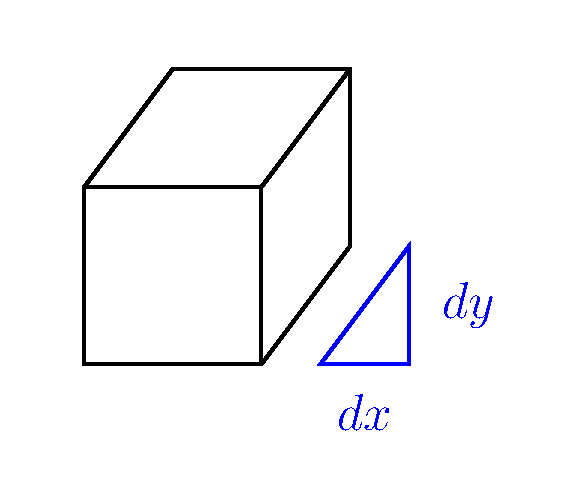
\includegraphics[height=4cm]{rubik-doc-figC.pdf}
%  \else
% 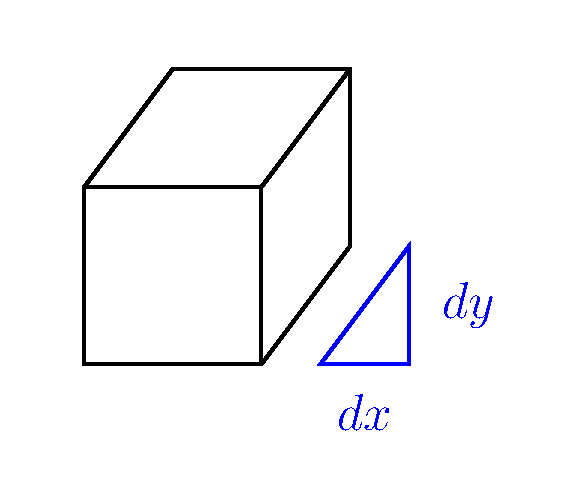
\includegraphics[height=4cm]{rubik-doc-figC.eps}
% \fi
% \vspace{-5mm}\caption{\label{fig:cubiedydx}Cubiedy and Cubiedx parameters} 
% \end{figure}
%
%  \DescribeMacro{\Cubiedy}
%  \DescribeMacro{\Cubiedx}
%  Minor  cubie configuration changes  can be effected 
%  by adjusting the Cubiedy and Cubiedx  values ($> 0$; no units)  
% shown in Figure~\ref{fig:cubiedydx}  via the two commands
% \begin{quote}
% \cmd{\Cubiedy\{\}} \\
% \cmd{\Cubiedx\{\}} 
% \end{quote}
% as shown in the following example.
%
% \bigskip
%
% \ShowCube{1.7cm}{1}{%
%   \Cubiedy{0.4}%
%   \Cubiedx{0.8}%
%   \DrawCubieRU{O}{Y}{G}% 
%  }
% \hspace{2cm}
% \begin{minipage}{0.6\textwidth}
%\begin{verbatim}
% \ShowCube{1.7cm}{1}{%
%   \Cubiedy{0.4}
%   \Cubiedx{0.8}
%   \DrawCubieRU{O}{Y}{G} 
%  }
%\end{verbatim}
% \end{minipage}
% 
% \bigskip
%
% {\noindent}Note that the  \textsc{front} face of the cubie is a unit square, 
% and the graphic origin of the cubie image is at the bottom left corner of the 
% \textsc{front} face (see also the section on Arrows: Section~\ref{sec:arrows}).
% The default  values of \cmd{\Cubiedy} and \cmd{\Cubiedx} are 0.4. 
%
%
%
%  \subsection{textCubie commands}
%
% \DescribeMacro{\textCubieRU}
% \DescribeMacro{\textCubieRD}
% \DescribeMacro{\textCubieLU}
% \DescribeMacro{\textCubieLD}
% For convenience, there are also four (smaller) `text' versions \textCubieRU{O}{Y}{G}   
%  of the  four \cmd{\DrawCubie} commands for use in ordinary text, as follows:
% \begin{quote}
%  \textCubieRU{O}{Y}{G} \ \ |\textCubieRU{O}{Y}{G}|
%
% \medskip
%
% \textCubieRD{O}{Y}{G} \ \  |\textCubieRD{O}{Y}{G}|     
%
% \medskip
%
% \textCubieLU{O}{Y}{G}  \ \ |\textCubieLU{O}{Y}{G}|
%
% \medskip
%
%  \textCubieLD{O}{Y}{G}  \ \  |\textCubieLD{O}{Y}{G}|  
% \end{quote}
% Note that these \cmd{\textCubieXY} commands are not influenced by the 
% \cmd{\Cubiedy}, \cmd{\Cubiedx} commands as their size is pre-set for text use. 
%
%
%
%  \subsection{DrawRubikCube commands}
%     \label{sec:drawrubikcubecommands}
%
%   \DescribeMacro{\DrawRubikCubeXY}
%   \DescribeMacro{\DrawRubikCubeF}
%   \DescribeMacro{\DrawRubikCubeSF}
% This  command  draws Rubik cubes  in one of four oblique 
% orientations or configurations as denoted by the following terminal 
% XY viewing-direction  codes:  RU~(RightUp),  RD~(RightDown), LU~(LeftUp), 
% LD~(LeftDown); two additional terminal codes are F~(Flat) and SF~(Semi-Flat). 
%  For~example, the command
%  \begin{quote}
%  \cmd{\DrawRubikCubeRU}
%  \end{quote}
% will draw a Rubik cube  as viewed from the RightUp direction (RU), as 
% shown in the following figure.
% 
% \bigskip
%
% \begin{minipage}{2.8cm}
% \begin{tikzpicture}[scale=0.7]
% \RubikCubeSolvedWY
% \DrawRubikCubeRU 
% \end{tikzpicture}%
% \end{minipage}
%   \hspace{5mm}
% \begin{minipage}{0.6\textwidth}
%\begin{verbatim}
% \RubikCubeSolvedWY
% \ShowCube{3cm}{0.7}{\DrawRubikCubeRU} 
%\end{verbatim}
% \end{minipage}
%
%  \bigskip
%
%  \DescribeMacro{\DrawRubikCubeF}
%  This command  draws the completely flat (F) format of the cube, as  shown in the following example.
%  
%  \bigskip
%  
%  \begin{minipage}{0.4\textwidth}
%  \centering
%  \begin{tikzpicture}[scale=0.4]
%  \RubikCubeSolvedWY
%  \DrawRubikCubeF
%  \node (U) at (1.5, 4.5)   [black]{\small\textsf{U}};
%  \node (D) at (1.5, -1.5)  [black]{\small\textsf{D}};
%  \node (L) at (-1.5, 1.5)  [black]{\small\textsf{L}};
%  \node (R) at (4.5, 1.5)   [black]{\small\textsf{R}};
%  \node (F) at (1.5, 1.5)   [black]{\small\textsf{F}};
%  \node (B) at (7.5, 1.5)   [black]{\small\textsf{B}};
%  \end{tikzpicture}%
%  \end{minipage}
%  \begin{minipage}{5cm}
%\begin{verbatim}
%  \RubikCubeSolvedWY
%  \ShowCube{5cm}{0.4}{\DrawRubikCubeF}
%\end{verbatim}
%  \end{minipage}
%  
%  \bigskip
%  
%  The addition of  text (numbers or letters) in the faces is 
%  straightforward---the origin of the 1-unit grid is located at the 
%  bottom left corner of the \textsc{front} face (orange here). 
%  The letters were placed using the following TikZ code inside the 
%  TikZ picture environment 
%  (remember TikZ commands require a terminal semi-colon~;).
%  
%\begin{verbatim}
%  \RubikCubeSolved
%  \ShowCube{5cm}{0.4}{%
%    \DrawRubikCubeF
%    \node (U) at (1.5, 4.5)   [black]{\small\textsf{U}};
%    \node (D) at (1.5, -1.5)  [black]{\small\textsf{D}};
%    \node (L) at (-1.5, 1.5)  [black]{\small\textsf{L}};
%    \node (R) at (4.5, 1.5)   [black]{\small\textsf{R}};
%    \node (F) at (1.5, 1.5)   [black]{\small\textsf{F}};
%    \node (B) at (7.5, 1.5)   [black]{\small\textsf{B}};
%    }
%\end{verbatim}
%  
%  \DescribeMacro{\DrawRubikCubeSF}
%  {\noindent}A useful `semi-flat' (SF) alternative format, which uses 
%  the standard RU  view of the cube  and  appends the three hidden 
%  sides (cf.,~Rokicki \textit{et~al.}, 2013),  is generated by the 
%  command \cmd{\DrawRubikCubeSF} as follows.
%  
%  \bigskip
%
%  \begin{minipage}{5cm}
%  \begin{tikzpicture}[scale=0.5]
%  \RubikCubeSolvedWY
%  \DrawRubikCubeSF
%  \node (B) at (5.5, 2.5)   [white]{\small\textsf{B}};
%  \end{tikzpicture}%
%  \end{minipage}
%  \begin{minipage}{5cm}
%\begin{verbatim}
%  \RubikCubeSolvedWY
%  \ShowCube{5cm}{0.5}{%
%     \DrawRubikCubeSF
%     \node (B) at (5.5, 2.5)  
%              [white]{\small\textsf{B}};
%     }
%\end{verbatim}
%  \end{minipage}
%  
% \bigskip
%
% Note that even in this configuration it is straight-forward to
% write text on the graphic, since the 2D width (on the page) of 
% the green  \textsc{right} face is exactly 1-unit, and the 
% bottom right-hand corner of the green face is raised exactly 1-unit
% (see Figure~\ref{fig:cubesquaregraph}).
% Consequently, since the origin of the  coordinate-grid is at the bottom left 
% corner of the \textsc{front} face (the orange face here), the ($x,y$) coordinates 
% of the centre of the  red \textsc{back} face are easily determined to be (5.5, 2.5). 
%  
%
%
%  \subsection{DrawRubikFace.. commands}
%  \label{sec:drawrubikfacecommands}
%
%
%  \DescribeMacro{\DrawRubikFaceUp}
%  \DescribeMacro{\DrawRubikFaceDown}
%  \DescribeMacro{\DrawRubikFaceLeft}
%  \DescribeMacro{\DrawRubikFaceRight}
%  \DescribeMacro{\DrawRubikFaceFront}
%  \DescribeMacro{\DrawRubikFaceBack}
%  \DescribeMacro{\DrawRubikFaceUpSide}
%  \DescribeMacro{\DrawRubikFaceDownSide}
%  \DescribeMacro{\DrawRubikFaceLeftSide}
%  \DescribeMacro{\DrawRubikFaceRightSide}
%  \DescribeMacro{\DrawRubikFaceFrontSide}
%  \DescribeMacro{\DrawRubikFaceBackSide}
% These commands draw the current state of a specified  face 
% (e.g.,~\cmd{\DrawRubikFaceUp}), or the face and all the associated sidebars
% (e.g.,~\cmd{\DrawRubikFaceUpSide}). These  commands  do \textsc{not} take any 
% arguments---for code see Section~\ref{sec:drawrubikfacecode}.
%
% \textsc{Note}: These commands  replace the earlier 
%  \cmd{\DrawFace...} commands  (see Section~\ref{sec:deprecated}).
%
%  For example, a simple way to  show the yellow-cross configuration in 
%  the  \textsc{up}~face would be to first define the colours using 
%  the \cmd{\RubikFaceUp} command, and then draw the \textsc{up} face 
%  using the  \cmd{\DrawRubikFaceUp} command, as follows:
%  
%  \bigskip
%
%  
%  \RubikFaceUp{X}{Y}{X}
%              {Y}{Y}{Y}
%              {X}{Y}{X}
%  \ShowCube{2.1cm}{0.7}{\DrawRubikFaceUp}
%  \hspace{1cm}
%  \begin{minipage}{0.6\textwidth}
%\begin{verbatim}
%  \RubikFaceUp{X}{Y}{X}
%              {Y}{Y}{Y}
%              {X}{Y}{X}
%  \ShowCube{2.1cm}{0.7}{\DrawRubikFaceUp}
%\end{verbatim}
%  \end{minipage}
%
%
%
%    \subsection[Drawing Sidebars (Face)]{Sidebars \& DrawRubikFaceXSide commands}
%      \label{sec:sidebars}
%
%
%  In the next  example we use the \cmd{\DrawRubikFaceUpSide} command to
%  draw the \textsc{up}~face and all its sidebars  in a cube  having 
%  a `solved' WY (White opposite Yellow) configuration.
%
%  \bigskip
%  
%  \RubikCubeSolvedWY
%  \ShowCube{1.6cm}{0.5}{\DrawRubikFaceUpSide}
%   \hspace{1cm}
%  \begin{minipage}{0.6\textwidth}
%\begin{verbatim}
%  \RubikCubeSolvedWY
%  \ShowCube{1.6cm}{0.5}{\DrawRubikFaceUpSide}
%\end{verbatim}
%  \end{minipage}
%
% \bigskip
% 
% \noindent\textbf{Short-hand versions}:  For convenience each of these commands 
% has an equivalent short-hand version generated by using just the first letter of the 
% face name and (where appropriate) the first letter of the word Side. For~example,
% \newline\cmd{\DrawRubikFaceR} $\equiv$  \cmd{\DrawRubikFaceRight},    
% \newline \cmd{\DrawRubikFaceRS} $\equiv$ \cmd{\DrawRubikFaceRightSide}, etc.
%
%
%
%
%
%    \subsection{Sidebar parameters}
%      \label{sec:sidebarparameters}
%
%  \DescribeMacro{\RubikSidebarWidth}
%  \DescribeMacro{\RubikSidebarLength}
%  \DescribeMacro{\RubikSidebarSep}
%  The default values (size) of the  sidebars are as follows:
%  width (0.3), length(1) and separation  from the square face (0.3) 
%  ---see Section~\ref{sec:sidebarcode} for the code. 
%  Note that the default value of the length of a cubie side is 1. 
%  These sidebar values (decimal values $\geq 0$; no units) can be 
%  changed from their default values using the three commands.
%  \begin{quote}
%  \cmd{\RubikSidebarWidth\{\}}\hspace{35.751pt}(default = 0.3)\\
%  \cmd{\RubikSidebarLength\{\}}\hspace{30pt}(default = 1.0)\\
%  \cmd{\RubikSidebarSep\{\}}\hspace{46.251pt}(default = 0.3)
%  \end{quote}
%  Values set in the document preamble will apply globally, while values 
%  set within a TikZ picture environment will apply only locally to that 
%  particular environment. Alternatively, one can keep the effect local
%  using braces (see below).
%
%  In the following example, we show the effect 
%  on the \textsc{up} face  and sidebars  of a normally solved (WY) cube 
%  after  dramatically changing  the sidebar width, length and separation
%  from the default values---compare with the previous image.  
%  For~convenience, we have used a pair of braces 
%  to keep the effect local to this example.
%  
%  \bigskip
%
%  {
%  \RubikCubeSolvedWY
%  \RubikSidebarWidth{0.8}
%  \RubikSidebarLength{0.5}
%  \RubikSidebarSep{0.7}
%  \ShowCube{2cm}{0.5}{\DrawRubikFaceUpSide}
%  }
%      \hspace{2cm}
%  \begin{minipage}{0.6\textwidth}
%\begin{verbatim}
%  {
%  \RubikCubeSolvedWY
%  \RubikSidebarWidth{0.8}
%  \RubikSidebarLength{0.5}
%  \RubikSidebarSep{0.7}
%  \ShowCube{2cm}{0.5}{\DrawRubikFaceUpSide}
%  }
%\end{verbatim}
%  \end{minipage}
%  
%  \bigskip
%  
%  Note also that changing the  sidebar-width or sidebar-separation 
%  values may well also change the surrounding white-space (use \cmd{\fbox} 
%  to visualise this) and may therefore require some fine-tuning of the 
%  minipage width setting in order to optimise  appearance. 
% 
%
%
%
%   \subsection[NoSidebar command]{\cmd{\NoSidebar} command}
%   \label{sec:nosidebar}
%
% \DescribeMacro{\NoSidebar}
% The  \cmd{\NoSidebar}\marg{colour-code}  command 
% (which takes a single colour code argument) 
% allows the user to disable the drawing of sidebars having a particular colour
% (for code see Section~\ref{sec:nosidebarcode}).
% Its action can be localised by placing the command inside an environment 
% (e.g.,~inside the \verb!\ShowCube! environment).
% Alternatively, the action of this  command can be disabled simply by writing it with an empty 
% argument, e.g.,~\verb!\NoSidebar{}!.
%
% This command is designed to facilitate the drawing of so-called 
% OLL (Orientate Last Layer) configurations,
% which are typically rendered  using the yellow face.
%
% For~example, the following figure uses the \verb!\DrawRubikFaceUpSide! command to 
% draw  the commonly encountered OLL configuration  known as the `yellow cross'
% (the remaining four yellow facelets associated with this layer are shown as sidebars).
% In this example, we first define the colours for the whole cube (grey), and then
% redefine the colours for the \textsc{up}~face and its four adjacent faces.
% Finally we draw the \textsc{up}~face and sidebars;  we also show  an alternative
% way of writing the facelet colour codes (ie without using the curly brackets).
%
% \bigskip
%
% \begin{minipage}{3cm}
% \RubikCubeGreyAll
% \RubikFaceUp XYX
%              YYY
%              XYX
% \RubikFaceFront YXY XXXXXX
% \RubikFaceRight XXY XXXXXX
% \RubikFaceBack  XXX XXXXXX
% \RubikFaceLeft  YXX XXXXXX
% \ShowCube{2.6cm}{0.6}{\DrawRubikFaceUpSide}
% \end{minipage}
% \hspace{4mm}
% \begin{minipage}{5cm}
% \begin{verbatim}
% \RubikCubeGreyAll
% \RubikFaceUp XYX
%              YYY
%              XYX
% \RubikFaceFront YXY XXXXXX
% \RubikFaceRight XXY XXXXXX
% \RubikFaceBack  XXX XXXXXX
% \RubikFaceLeft  YXX XXXXXX
% \ShowCube{2.6cm}{0.6}{\DrawRubikFaceUpSide} 
% \end{verbatim}
% \end{minipage}
% \bigskip
%
% {\noindent}However, we can greatly improve the OLL image by 
% disabling the drawing of all the grey (X) sidebars by using the 
% \verb!\NoSidebar{X}! command as follows (here we have placed the 
% \verb!\NoSidebar{X}! command inside the \verb!\ShowCube! environment 
% in order to limit its action locally). Note also that this time we 
% have used the short-hand US (UpSide) version of the 
% \cmd{\DrawRubikFaceUpSide} command.
% 
% \bigskip
%
% \begin{minipage}{3cm}
% \RubikCubeGreyAll
% \RubikFaceUp XYX
%              YYY
%              XYX
% \RubikFaceFront YXY XXXXXX
% \RubikFaceRight XXY XXXXXX
% \RubikFaceBack  XXX XXXXXX
% \RubikFaceLeft  YXX XXXXXX
% \ShowCube{2.6cm}{0.6}{\NoSidebar{X}\DrawRubikFaceUS}
% \end{minipage}
% \hspace{4mm}
% \begin{minipage}{5cm}
% \begin{verbatim}
% \RubikCubeGreyAll
% ...
% ...
% \ShowCube{2.6cm}{0.6}{\NoSidebar{X}%
%                       \DrawRubikFaceUS%
%                      }
% \end{verbatim}
% \end{minipage}
% 
% \bigskip
%
%
%
%    \subsection[Drawing Sidebars (Cube)]{Cube sidebars \& DrawRubikCubeSidebar commands}
%      \label{sec:sidebarscube}
%
% 
%
%
% Cube sidebars are drawn adjacent to cube edges which are  
% defined by the two faces forming the edge.
% Thus the BR (Back-Right) sidebar is placed adjacent to the 
% edge formed by the \textsc{back} and \textsc{right} faces. 
%
% Since the cube orientation (view direction; RU, RD, LU, LD) 
% determines which sidebars are visible, the  command for drawing 
% the sidebar (\texttt{DrawRubikCubeSidebar..}) also needs to 
% incorporate the view direction. The command takes 
% two mandatory  arguments: the first is the pair of face codes defining the edge (XX); 
% the second is the  view direction, as follows:
% \begin{quote}
% \cmd{\DrawRubikCubeSidebarXX}\marg{view direction} 
%
%  \textsc{example:} \verb!\DrawRubikCubeSidebarRB{LD}!
% \end{quote}
% Note that the pair of face codes  are  order \textit{independent}, 
% and hence can be written in any order, which makes remembering the commands very easy.
% 
% Note also that at present commands are only available for the 
% eight sidebars which are parallel to X,Y axes, as these seem 
% to be the most useful.
%
% In the following example, we input a previously saved cube state 
% (in the file \texttt{cubestate-A.tex}) and draw the cube and the 
% four main sidebars (BR, BD, FL, FU)  visible from the RD view direction. 
%         
% \bigskip
%
% \RubikFaceUp{O}{G}{Y}{B}{B}{O}{R}{B}{G}%
% \RubikFaceDown{Y}{R}{B}{R}{W}{O}{W}{Y}{R}%
% \RubikFaceLeft{Y}{G}{W}{W}{Y}{R}{O}{W}{B}%
% \RubikFaceRight{B}{B}{B}{W}{G}{O}{R}{G}{W}%
% \RubikFaceFront{G}{R}{O}{Y}{R}{O}{R}{G}{G}%
% \RubikFaceBack{O}{W}{W}{Y}{O}{Y}{Y}{B}{G}%
% \ShowCube{4cm}{0.6}{
%        \DrawRubikCubeRD
%         \DrawRubikCubeSidebarBR{RD}
%         \DrawRubikCubeSidebarBD{RD}
%         \DrawRubikCubeSidebarFL{RD}
%         \DrawRubikCubeSidebarFU{RD}
%         }
% \begin{minipage}{5cm}
%\begin{verbatim}
% \input{cubestate-A.tex}
% \ShowCube{3cm}{0.6}{
%         \DrawRubikCubeRD
%         \DrawRubikCubeSidebarBR{RD}
%         \DrawRubikCubeSidebarBD{RD}
%         \DrawRubikCubeSidebarFL{RD}
%         \DrawRubikCubeSidebarFU{RD}
%         }
%\end{verbatim}
% \end{minipage}         
%
%\bigskip
%
%
%
% 
%  \subsection{DrawRubikFlat commands}
%  \label{sec:drawrubikflatcommands}
%
%  \DescribeMacro{\DrawRubikFlatUp}
%  \DescribeMacro{\DrawRubikFlatDown}
%  \DescribeMacro{\DrawRubikFlatLeft}
%  \DescribeMacro{\DrawRubikFlatRight}
%  \DescribeMacro{\DrawRubikFlatFront}
%  \DescribeMacro{\DrawRubikFlatBack}
%  The  \cmd{\DrawRubikFlat..}\marg{x}\marg{y} commands draw a `flat' square 
%  representation of a specified face,  located such that its 
%  bottom left corner  is positioned at ($x,y$). 
%  Each command (except \cmd{\DrawRubikFlatFront}) takes two arguments, 
%  namely the  X-coordinate  and Y-coordinate of the bottom left 
%  corner of the  face.  This ($x,y$) pair allows the user to position
%  the face (see Section~\ref{sec:codedrawrubikflatcommands} for the code).
%
%  These commands are designed to supplement the \cmd{\DrawRubikCube...} commands and 
%  allow hidden faces to be represented. 
%
%  Note also that the \cmd{\DrawRubikFlatFront} command currently takes \textit{no} 
%  arguments, since by definition the bottom left corner of this face is 
%  always at (0,0),  and there seems to be no reason (just now) for 
%  this face to have the  ($x,y$) facility.
%
%  \textsc{usage}:\ The following example uses the command \verb!\DrawRubikFlatBack{4}{1}! to
%  append the \textsc{back} face to the side of a 3D  cube. Note that since 
%  the coordinates of the bottom/back/right corner of the cube rendered by the 
%  command \cmd{\DrawRubikCubeRU} is (4,1) 
%  (see Section~\ref{sec:coordinates}), we can position the 
%  lower/left corner of the \textsc{back} face at this point using the command
%  \verb!\DrawRubikFlatBack{4}{1}! as follows: 
%
%  \bigskip
%  
%  \begin{minipage}{0.4\textwidth}
%  \centering
%  \RubikCubeSolvedWY
%  \begin{tikzpicture}[scale=0.5]
%  \DrawRubikCubeRU
%  \DrawRubikFlatBack{4}{1}
%  \end{tikzpicture}%
%  \end{minipage}
%  \begin{minipage}{5cm}
%\begin{verbatim}
%  \RubikCubeSolvedWY
%  \ShowCube{3cm}{0.5}{%
%     \DrawRubikCubeRU
%     \DrawRubikFlatBack{4}{1}
%  }
%\end{verbatim}
%  \end{minipage}
%
%
%      \subsection[DrawNCube]{DrawNCube (NxNxN)}
%      \label{sec:NCube}
% 
%  \DescribeMacro{\DrawNCubeAll} 
%  An `NCube' is  a solved NxNxN cube drawn from the RU direction; 
%  (i.e.,~only shows faces \textsc{up}, \textsc{front}, \textsc{right}). 
%  The cubie colours of each face are All the same.
%  \begin{quote}
%    \cmd{\DrawNCubeAll\{N\}\{Xcolour\}\{Ycolour\}\{Zcolour\}}.
%  \end{quote}
%  This command takes four ordered parameters (N, X, Y, Z)---the number 
%  (integer; $N>0$) of cubies along an edge, followed by three face 
%  colours in XYZ order.
%  Since the viewpoint is only from the RU direction, the  three colour 
%  parameters are: X(Right), Y(Up), Z(Front).
%  
%  \bigskip
%  
%  \begin{minipage}{0.3\textwidth}
%  \begin{tikzpicture}[scale=0.5]
%     \DrawNCubeAll{5}{O}{Y}{G}
%  \end{tikzpicture}%
%  \end{minipage}
%  \begin{minipage}{0.5\textwidth}
%\begin{verbatim}
% \ShowCube{3.5cm}{0.5}{\DrawNCubeAll{5}{O}{Y}{G}}
%\end{verbatim}
%  \end{minipage}
%
%
%
%
%   \section[ShowSequence command]{\cmd{\ShowSequence} command}
%   \label{sec:showsequence}
%
% \DescribeMacro{\ShowSequence}
% \DescribeMacro{\ShowSequenceF}
% \DescribeMacro{\ShowSequencef}
% The  \cmd{\ShowSequence}\marg{separator}\marg{font-code}\marg{sequence}  command 
% typesets a comma-separated sequence of rotation  
% codes---for code see Section~\ref{sec:codeshowsequence}.
% Appending an `F' to the command-name (\cmd{\ShowSequenceF}) results in an fbox around
% the whole output (cf.~the \cmd{\ShowCubeF} command). 
% Appending a lower-case `f' to the command-name (\cmd{\ShowSequencef}) generates fboxs around
% \textit{each element} in the output (these two forms can be helpful when checking white space). 
%
% The \cmd{\ShowSequence} command takes three mandatory arguments: 
% the first is the separator  (\verb!#1!), 
% the second is  the font or style code (\verb!#2!), 
% and third is a comma-separated  sequence of Rubik  rotation codes (|#3|).
%
% The separator (e.g.,~comma) used for typesetting the sequence can be specified 
% (or just omitted---i.e.,~an empty bracket);
% the sequence can be either a named sequence (i.e.,~encoded as a macro) or just a 
% comma separated sequence of  rotation codes.
% 
% \noindent\textsc{usage}:
% The following command  displays the rotation sequence  F, R, U, Rp, Up, using 
% the \verb!\rr! encoding and  comma \& space separated.
%
% \medskip
%
% \verb!\ShowSequence{,\ }{\rr}{F,R,U,Rp,Up}! \ \ $\rightarrow$ \ \ \ShowSequence{,\ }{\rr}{F,R,U,Rp,Up}
%
% \medskip
%
% Remember that if you want a  very long  sequence to break automatically 
% at the line-ends, then you need to include at least one space between 
% the sequence elements, either with or without a comma; for this the 
% separator argument needs to include a space, i.e.,~something like 
% \verb!{,\ }! or \verb!{\ }!  or just \verb!{ }! perhaps.
%
%
% For~example, the following commands typeset the comma-separated 
% rotation sequence U,D,Lp,R  using different separators and fonts. 
% For convenience, we start by encoding  the sequence as the macro \verb!\myseq!.
%
%
% \newcommand{\myseq}{U,D,Lp,R}
%
% \medskip\noindent\verb!\newcommand{\myseq}{U,D,Lp,R}!
%
% \medskip\noindent\verb!\ShowSequence{,}{\texttt}{\myseq}! \ $\longrightarrow$ \  \ShowSequence{,}{\texttt}{\myseq}
%
% \medskip\noindent\verb!\ShowSequence{,}{\rr}{\myseq}! \ $\longrightarrow$ \  \rr{U},\rr{D},\rr{Lp},\rr{R} 
%
% \medskip\noindent\verb!\ShowSequence{}{\rrh}{\myseq}! \ $\longrightarrow$ \  \rrh{U}\rrh{D}\rrh{Lp}\rrh{R}
%
% \medskip\noindent\verb!\ShowSequence{\ }{\rrh}{\myseq}! \ $\longrightarrow$ \  \rrh{U}\ \rrh{D}\ \rrh{Lp}\ \rrh{R}
% 
% \medskip\noindent\verb!\ShowSequence{,\ }{\textRubik}{\myseq}! \ $\longrightarrow$ \  \textRubik{U},\ \textRubik{D},\
% \textRubik{Lp},\ \textRubik{R}
% 
%
%
% 
% \subsection{Trailing digits}
%
%  Note that the commands  \verb!\rr!, \verb!\rrh!, \verb!\Rubik! 
%  and \verb!\textRubik!  will fail for  rotation codes which 
%  have a trailing digit, e.g.,~R2, Dp3 (so-called `short' codes), since the 
%  \verb!\ShowSequence! macro currently only reads the whole string  between pairs of 
%  commas (i.e.,~it does not \textit{interpret}  strings like R2 $\rightarrow$ R,R etc.). 
%  However, if you just want to `see' the text, then the standard \LaTeX\ typewriter command 
%  \verb!\texttt!  will typeset the text correctly, as you would expect 
% (but using the \texttt{tt} font of course). 
% 
%  A useful `work-around' for this limitation  is provided by the \verb!\RubikRotation{}! 
%  command\,\footnote{Using the \texttt{--shell-escape} command-line option
%  with the \LaTeX\ engine---see Section~\ref{sec:rubikrotation}.} 
%  (part of the \textsc{rubikrotation} package), since this returns  (via the Perl program  
%  \texttt{rubikrotation.pl}) an extended (`long') form of a given sequence in which 
%  any `short' rotation codes are converted into their separate (atomic) long-form rotation codes; 
%  the associated string  is  \verb!\SequenceLong!. 
%  In fact  three different forms of the sequence are returned, as shown below.
% 
%  For~example, consider the following short-form sequence  L,R,D2,L3, and denote 
%  it as `seqA' as follows: \verb!\newcommand{\seqA}{[seqA],L,R,D2,L3,<test>}!.
%  In~this case  D2,L3, and the name `seqA'  fail to be typeset when using 
%  the \verb!\rr! font  with the \verb!\ShowSequence! command  
%  (notice there are lots of  commas with nothing between them), 
%  while \cmd{\texttt} does work, as follows:
% 
%  \newcommand{\seqA}{[seqA],L,R,D2,L3,<test>}
% 
%  \medskip\noindent\verb!\newcommand{\seqA}{[seqA],L,R,D2,L3,<test>}!
%
% \medskip\noindent\verb!\ShowSequence{,}{\rr}{\seqA}! \ $\longrightarrow$ \  \ShowSequence{,}{\rr}{\seqA}
%
% \medskip\noindent\verb!\ShowSequence{,}{\texttt}{\seqA}! \ $\longrightarrow$ \  \ShowSequence{,}{\texttt}{\seqA}
%
% \medskip
% 
% However, if we now run the command \verb!\RubikRotation{\seqA}! we shall then have 
% at our disposal the following four  strings:
%
% \medskip
%
% \verb!\SequenceInfo   = ! test
%
% \verb!\SequenceName   = ! seqA
% 
% \verb!\SequenceShort  = ! L,R,D2,L3
% 
% \verb!\SequenceLong   = ! L,R,D,D,L,L,L
%
% \medskip
% 
% {\noindent}and therefore have full control over  typesetting    rotation sequences.
% This approach therefore  offers sufficient flexibility for most purposes.
% For~example, if  we now write the command \verb!\ShowSequence{,}{\rr}{\SequenceLong}!
% we obtain
% 
% \medskip\noindent\verb!\ShowSequence{,}{\rr}{\SequenceLong}! \ $\longrightarrow$ \ 
% \ShowSequence{,}{\rr}{L,R,D,D,L,L,L}
%
% \medskip
%
% In practice, any trailing digit is converted (modulo~4) and expanded accordingly, the details being
% copied to the log-file. For~example, if one writes the command
% \cmd{\RubikRotation\{[test],R,D28978\}}, then since $28978 \equiv 2$\,(modulo~4) then \cmd{\SequenceLong} 
% will be returned containing the string |R,D,D|. The associated entries in the log-file  are
% as  follows:
%\begin{verbatim}
%...rotation R OK
%...Expanding D28978 (28978 = 2 mod 4) ...
%...rotation D OK (= Dp3)
%...rotation D OK (= Dp3)
%...writing new Rubik state to file rubikstateNEW.dat
%...SequenceName = test
%...SequenceShort = R,D28978
%...SequenceLong = R,D,D
%\end{verbatim}
%
%
%
%  \section{SequenceBrace commands}
%  \label{sec:sequencebrace}
%
%  \DescribeMacro{\SequenceBraceA} 
%  \DescribeMacro{\SequenceBraceB} 
%  \DescribeMacro{\SequenceBraceAF} 
%  \DescribeMacro{\SequenceBraceBF} 
% The  \cmd{\SequenceBraceX}\marg{name}\marg{sequence}  command 
% is a tool for displaying a named sequence using a brace. The trailing~A 
% denotes that the brace is placed Above the sequence; the trailing~B denotes 
% the brace is Below the sequence.
% Appending an `F' to the command-name (e.g.,~\cmd{\SequenceBraceAF}) results 
% in a surrounding  fbox (cf.~the \cmd{\ShowCubeF} command). 
% For the code see Section~\ref{sec:sequencebracecode}.
%
% {\noindent}Thus \verb!\SequenceBraceB{myseq}{U,D,L,R}! generates 
% \ \SequenceBraceB{myseq}{U,D,L,R}. 
%
% {\noindent}A typical example of its use might be:
%
% \bigskip
%
%\noindent%
%\RubikCubeSolvedWY%
%\ShowCube{1.6cm}{0.4}{\DrawRubikCubeRU}%
%\quad\SequenceBraceA{fourspot}{\ShowSequence{}{\Rubik}{F,F,B,B,U,Dp,R,R,L,L,U,Dp}}%
%\quad$\longrightarrow$\quad%
%\RubikFaceFront{R}{R}{R}%
%               {R}{O}{R}%
%               {R}{R}{R}%
%\RubikFaceRight{B}{B}{B}%
%               {B}{G}{B}%
%               {B}{B}{B}%
%\ShowCube{1.6cm}{0.4}{\DrawRubikCubeRU}%
%
%
% \bigskip
%
% {\noindent}which was generated by the following code, showing that the \cmd{\ShowSequence}
% command can be used as an argument for the \cmd{\SequenceBraceA} command:
%\begin{verbatim}
%\newcommand{\fourspot}{[fourspot],F2,B2,U,Dp,R2,L2,U,Dp}%
%\noindent%
%\RubikCubeSolvedWY%
%\ShowCube{1.6cm}{0.4}{\DrawRubikCubeRU}%
%\RubikRotation{\fourspot}%
%\quad\SequenceBraceA{\SequenceName}{%
%                     \ShowSequence{}{\Rubik}{\SequenceLong}}%
%\quad$\longrightarrow$\quad%
%\ShowCube{1.6cm}{0.4}{\DrawRubikCubeRU}%
%\end{verbatim}
% Note (1)~that the `fourspot' listing is included in the \textsc{rubikpatterns} package, and 
% (2)~the \cmd{\RubikRotation} command requires using the \texttt{--shell-escape} command-line 
% option  with the \LaTeX\ engine---see Section~\ref{sec:rubikrotation} for details.
%
%
%
%        \section{Arrows}
%        \label{sec:arrows}
%  
%  The \rubikcube\ package does not offer any special commands for drawing 
%  arrows since it is straightforward just to include the appropriate TikZ
%  `draw' commands in the \texttt{tikzpicture} environment (i.e.,~in our 
%   own \cmd{\ShowCube} environment).
%  
%  In order to facilitate using the standard TikZ `draw' commands
%  the  graphic grid origin of  Rubik cube images  is located at the bottom left corner 
%  of the \textsc{front} face (see also Section~\ref{sec:coordinates} for details of the 
%  cube's coordinate  system). Similarly,  single face images  (e.g.,~drawn using the 
%  \cmd{\DrawRubikFace..} or \cmd{\DrawRubikFlat..}  commands etc.) and also Sidebars, have 
%  their  grid origin at the bottom left corner of the face.
%  Consequently the start and finish coordinates for any arrow or line are 
%  easy to determine.  
%  
%  \begin{figure}[hbt]
%     \centering
%  \ifpdf
%     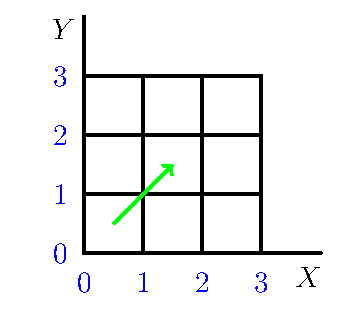
\includegraphics[height=3cm]{rubik-doc-figE.pdf}
%  \fi
%
%  \parbox{9cm}{%
%    \caption{\label{fig:facegraph}Grid showing the positive coordinates 
%   associated with \textsc{front} face of a cube image, or of a face-only image.} 
%   }%
%  \end{figure}
%  
% \medskip
%
%  For~example, Figure~\ref{fig:facegraph}  shows  a green
%   arrow drawn from the centre of the lower-left cubie $(0.5, 0.5)$  to the centre of 
%  middle cubie $(1.5, 1.5)$.
%  To do this  we  just include  the following TikZ  command (remember that  TikZ 
%  commands require a terminal semicolon):
%  \begin{quote}
%\begin{verbatim}
%  \draw[->,color=green] (0.5,0.5) -- (1.5, 1.5);
%\end{verbatim}
%  \end{quote}
%
%  The following example shows the  cubie movement in the \textsc{up} face 
%  generated by the rotation sequence \rrF\rrR\rrU\rrRp\rrUp\rrFp.
%  The magenta arrows indicate movement \textit{with} cubie rotations, 
%  while the black arrow indicates movement \textit{without} rotation.
%  This example also highlights the fact that when there are several arrows, 
%  the start and end positions often need to be offset slightly away from cubie centres.
%  
%  \bigskip
%  \noindent
%  \RubikCubeSolvedWY
%  \ShowCube{2.5cm}{0.7}{%
%    \DrawRubikFaceUp
%    \draw[->,thick,color=magenta] (1.5,0.5) -- (2.4, 1.4);
%    \draw[->,thick] (2.5,1.5) -- (1.6, 2.4);
%    \draw[->,thick,color=magenta] (1.3, 2.3) -- (1.3, 0.5);
%    \draw[<->,thick,color=magenta] (0.5,2.6) -- (2.5, 2.6);
%    \draw[<->,thick,color=magenta] (0.5,0.3) -- (2.5, 0.3);
%  }
%  \begin{minipage}{0.6\textwidth}
%\begin{verbatim}
%  \RubikCubeSolvedWY
%  \ShowCube{2.5cm}{0.7}{%
%    \DrawRubikFaceUp
%    \draw[->,thick,color=magenta] (1.5,0.5) -- (2.4, 1.4);
%    \draw[->,thick] (2.5,1.5) -- (1.6, 2.4);
%    \draw[->,thick,color=magenta] (1.3, 2.3) -- (1.3, 0.5);
%    \draw[<->,thick,color=magenta] (0.5,2.6) -- (2.5, 2.6);
%    \draw[<->,thick,color=magenta] (0.5,0.3) -- (2.5, 0.3);
%    }
%\end{verbatim}
%  \end{minipage}
%  
%  \bigskip
%  Since the coordinates shown in Figure~\ref{fig:facegraph} extend 
%  outwards in all directions, they can also be used as a guide for drawing 
%  arrows (or other structures) outside this 3x3 `face' square. 
%  The origin is at lower left corner of the face.
%
%  In the following example, we input a Rubik cube configuration 
%  (previously saved as the file \texttt{CubeFour.tex} 
%  (see the \textsc{rubikrotation} package documentation for details)\footnote{See also 
%  the `SaveRubikState' example  in the file \texttt{RubikExamples.pdf}.}, and 
%  draw an arrow to highlight a yellow  side facelet.
%  
%  \bigskip 
%  \noindent
%  \RubikCubeGreyAll
%  \RubikFaceUp    OYG YYY BYY
%  \RubikFaceFront YRR XXXXXX
%  \RubikFaceRight GOO XXXXXX
%  \RubikFaceBack  YBB XXXXXX
%  \RubikFaceLeft  YGR XXXXXX
%  \ShowCube{2.2cm}{0.5}{\DrawRubikFaceUpSide%
%             \draw[->,ultra thick,color=green] (2.5,5) -- (2.5, 4);
%              }
%  \begin{minipage}{0.6\textwidth}
%\begin{verbatim}
%  \input{CubeFour.tex}
%  \ShowCube{2.2cm}{0.5}{\DrawRubikFaceUpSide%
%       \draw[->,ultra thick,color=green] (2.5,5) -- (2.5, 4);
%       }
%\end{verbatim}
%  \end{minipage}
%  
%  \bigskip
%  
%  {\noindent}The following example shows an arrow on the Rubik cube. 
%  The origin of coordinates is at the bottom left corner of the 
%  \textsc{front} face (see Section~\ref{sec:coordinates}).
%  
%  \bigskip
%  \noindent
%  \begin{minipage}{2.8cm}
%  \centering
%  \begin{tikzpicture}[scale=0.7]
%  
%  \RubikFaceFront{O}{O}{O}
%                 {O}{O}{X}
%                 {X}{O}{X}
%  
%  \RubikFaceRight{G}{G}{G}
%                 {X}{G}{G}
%                 {X}{X}{X}
%  
%  \RubikFaceDown {X}{G}{X}
%                 {X}{Y}{X}
%                 {X}{X}{X}
%  
%  \DrawRubikCubeRD
%  \draw[ultra thick,->,color=blue] 
%            (1.5,0.5) -- (2.5, 1.5);
%  \end{tikzpicture}%
%  \end{minipage}
%     \hspace{1cm}
%  \begin{minipage}{0.6\textwidth}
%\begin{verbatim}
% \RubikFaceFront{O}{O}{O}
%                {O}{O}{X}
%                {X}{O}{X}
%  
% \RubikFaceRight{G}{G}{G}
%                {X}{G}{G}
%                {X}{X}{X}
%  
% \RubikFaceDown {X}{G}{X}
%                {X}{Y}{X}
%                {X}{X}{X}
% \ShowCube{3cm}{0.7}{%  
%    \DrawRubikCubeRD
%    \draw[ultra thick,->,color=blue] 
%                (1.5,0.5) -- (2.5, 1.5);  
%    }
%\end{verbatim}
%  \end{minipage}
%
% \bigskip
%
% In the following example we use a blue circle to highlight a corner cubie
% to be rotated into the top layer. Note we also use the command
% \verb!\DrawRubikCubeSidebarFD{RU}!  to draw the sidebar along 
% the FD (Front-Down) edge, and show the colour of the hidden facelet
% of the  corner-cubie.
%
% \bigskip
%
% \noindent%
% \RubikCubeGreyWY
% \RubikFaceUp{X}{W}{X}%
%             {W}{W}{W}%
%             {W}{W}{X}%
% \RubikFaceDown{X}{X}{O}{X}{X}{X}{X}{X}{X}%
% \RubikSliceBottomR{X}{X}{W}{G}{X}{X}%
% \ShowCube{2.5cm}{0.5}{%
%   \DrawRubikCubeRU
%   \DrawRubikCubeSidebarFD{RU}
%   \draw[ultra thick,->,color=blue] (2.5,0.5) -- (2.5, 2.5);
%   \draw [color=blue, thick] (2.7, 0.3)  circle (1.3);
% }%
%    \hspace{3mm}
% \begin{minipage}{0.6\textwidth}
%\begin{verbatim}
% \RubikCubeGreyWY
% \RubikFaceUp{X}{W}{X}
%             {W}{W}{W}
%             {W}{W}{X}
% \RubikFaceDown{X}{X}{O}{X}{Y}{X}{X}{X}{X}%
% \RubikSliceBottomR{X}{X}{W}{G}{X}{X}
% \ShowCube{2.5cm}{0.5}{%
%   \DrawRubikCubeRU
%   \DrawRubikCubeSidebarFD{RU}
%   \draw[ultra thick,->,color=blue] 
%                              (2.5,0.5) -- (2.5, 2.5);
%   \draw [color=blue, thick] (2.7, 0.3)  circle (1.3);
%   }%
%\end{verbatim}
% \end{minipage}
%
%
%
%
%
% \section{Final example}
%
% We now present, as a final example, the code used to draw the  front page 
% figure\,\footnote{This is a well-known sequence of order 6 used to  cycle three
% edge cubies; it is used to generate the `cross' configuration  in the final layer
% when solving the cube. Here we are performing the sequence on  a `solved' cube, 
% since this allows you  to see how the three edge cubies  move, and either 
% flip (magenta arrows) or do not flip (black arrow).}. 
% This code uses  the \cmd{\RubikRotation} command (from the \textsc{rubikrotation}
%  package), and therefore the \LaTeX\ engine needs to be run using the 
% \verb!--shell-escape!  command-line switch (see  Section~\ref{sec:rubikrotation} for details).
%
% \bigskip
%
% \noindent\hfil%
% \RubikCubeSolvedWY%
% \ShowCube{1.6cm}{0.4}{\DrawRubikCubeRU}%
% \quad\ShowCube{1.6cm}{0.4}{%
%    \DrawRubikFaceUpSide
%    \draw[thick,->,color=magenta] (1.5,0.5) -- (2.4, 1.4);
%    \draw[thick,->] (2.5,1.5) -- (1.6, 2.4);
%    \draw[thick,->,color=magenta] (1.3, 2.3) -- (1.3, 0.5);
%    \draw[thick,<->,  color=blue] (0.5,2.6) -- (2.5, 2.6);
%    \draw[thick,<->,  color=blue] (0.5,0.3) -- (2.5, 0.3);
%   }%
% \quad\Rubik{F}\Rubik{R}\Rubik{U}\Rubik{Rp}\Rubik{Up}\Rubik{Fp}%
%  \quad$\longrightarrow$%
%  \RubikFaceUp   WWB WWOWRB%
%  \RubikFaceBack RGG XXXXXX%
%  \RubikFaceLeft RBO XXXXXX%
% \RubikFaceFront GWO XXXXXX%
% \RubikFaceRight WWW XXXXXX%
% \quad\ShowCube{1.6cm}{0.4}{\DrawRubikFaceUpSide}
% \hfil%
%
%
% \bigskip  
%
%\begin{verbatim}
% \noindent\hfil%
% \RubikCubeSolvedWY%
% \ShowCube{1.6cm}{0.4}{\DrawRubikCubeRU}%
% \quad\ShowCube{1.6cm}{0.4}{%
%    \DrawRubikFaceUpSide%
%    \draw[thick,->,color=magenta] (1.5,0.5) -- (2.4, 1.4);
%    \draw[thick,->] (2.5,1.5) -- (1.6, 2.4);
%    \draw[thick,->,color=magenta] (1.3, 2.3) -- (1.3, 0.5);
%    \draw[thick,<->,  color=blue] (0.5,2.6) -- (2.5, 2.6);
%    \draw[thick,<->,  color=blue] (0.5,0.3) -- (2.5, 0.3);
%    }%
% \RubikRotation{F,R,U,Rp,Up,Fp}%
% \quad\ShowSequence{}{\Rubik}{\SequenceLong}\quad$\longrightarrow$%
% \ShowCube{1.6cm}{0.4}{\DrawRubikFaceUpSide}%
% \hfil
%\end{verbatim}
%
%
%
%     \subsection[Without using {\textbackslash}RubikRotation]{Without using \cmd{\RubikRotation}}
%
% If you really need to draw the above figure \textit{without}  using 
% the \textsc{rubikrotation}  package (as we had to in order to write 
% this particular document) then  you would need to  replace the 
% commands
%\begin{verbatim}
% \RubikRotation{F,R,U,Rp,Up,Fp}
% \ShowSequence{,}{\Rubik}{\SequenceLong} \ \ \ $\longrightarrow$
% \ShowCube{2cm}{0.4}{\DrawRubikFaceUpSide}
%\end{verbatim}
% with the following commands:
%
%\begin{verbatim}
% \Rubik{F}\Rubik{R}\Rubik{U}\Rubik{Rp}\Rubik{Up}\Rubik{Fp}
% \ \ \ $\longrightarrow$
%  \RubikFaceUp   WWB WWOWRB
%  \RubikFaceBack RGG XXXXXX
%  \RubikFaceLeft RBO XXXXXX
% \RubikFaceFront GWO XXXXXX
% \RubikFaceRight WWW XXXXXX
% \quad\ShowCube{1.6cm}{0.4}{\DrawRubikFaceUpSide}
% \hfil
%\end{verbatim}
%
%
%
%
%
%     \section{Deprecated commands}
%     \label{sec:deprecated}
%
% 
% The  \cmd{\DrawRubikLayerFace..}    and   \cmd{\DrawRubikLayerSide..} 
% are now deprecated; they were found to be 
% confusing  since (a)~they both drew faces \textit{and}  took colour arguments
% for facelets, and (b)~they did not update the internal colour state of a 
% cube or face---i.e.,~their colouring  was simply a local `painting' action 
%  without memory. 
%   They   have both been superseded  by the more versatile 
%  \cmd{\DrawRubikFace..}\ commands (see Section~\ref{sec:drawrubikfacecommands}).
%
% The \cmd{\RubikSide..} commands are also  deprecated, since they duplicated 
% some of the function of the  \cmd{\RubikFace..}\ commands.
%
% The earlier \cmd{\DrawFace..}\ (v4) and  \cmd{\DrawFlat..}\ (v3) commands
% are also deprecated since they lacked the Rubik or Two keyword 
% (see Sections~\ref{sec:rubikandtwo} and \ref{sec:drawrubikfacecommands}).
%
%  \medskip
%
% {\noindent}Summary of all deprecated commands (and their current versions) since v3.
%
% \smallskip
%
% \begin{supertabular}[ll]{p{4cm} p{6cm}}
% \verb!\DrawRubikCubeFlat!   & $\rightarrow$ \hspace{0.5cm}    \verb!\DrawRubikCubeSF! \ (Semi-Flat) \\
% \verb!\DrawRubikFlat!       & $\rightarrow$ \hspace{0.5cm}    \verb!\DrawRubikCubeF! \ \ (Flat) \\ 
% \verb!\DrawFace..!       & $\rightarrow$ \hspace{0.5cm}    \verb!\DrawRubikFace..!   \\
% \verb!\DrawFlat..!       & $\rightarrow$ \hspace{0.5cm}    \verb!\DrawRubikFlat..!   \\
% \verb!\DrawFlat..Side!    & $\rightarrow$ \hspace{0.5cm}    \verb!\DrawRubikFace..Side! \\
% \verb!\DrawRubikLayerFace..! & $\rightarrow$ \hspace{0.5cm}    \verb!\DrawRubikFace..!  \\
% \verb!\DrawRubikLayerSide..!  & $\rightarrow$ \hspace{0.5cm}    \verb!\DrawRubikFace..!  \\
% \end{supertabular}
%
%
%
%
%  \section{Known limitations}
%
% Please contact the authors regarding any ideas for improvement, errors, 
% problems or shortcomings etc. 
%
% \begin{itemize} 
%  
%  \item  Note that  the rotation hieroglyphs are optimised for a 10pt font
%  and  do  not  scale  with document  font size. However, they do work well  in 
%  conjunction with the standard 11pt and 12pt document fonts sizes. Nevertheless, 
%  the font size can of course be changed by renewing the font command 
%  (see Section~\ref{sec:rubikfont} for details).
%
%  \item The sidebars cannot be arbitrarily positioned (note: hidden 
%  faces can be arbitrarily positioned).
% 
% \end{itemize}
%
%
%
% 
%     \section{Change history}
%
% \begin{itemize}
%
% \item Version 5 (February 2018)
%
%   -- Removed some now unnecessary commands (see Section~\ref{sec:deprecated}) 
%      and made some of the internal code a bit more efficient.
%
%  ---Added two new `grey' commands: \cmd{\RubikCubeGreyWY} and \cmd{\RubikCubeGreyWB} 
%      (so as to complement  the related \cmd{\RubikCubeSolvedXX} commands).
%
%  ---Bugfix: added a pair of containing braces around the \cmd{\ifthenelse..} command 
%  used by the \cmd{\ShowSequence} command (for code see Section~\ref{sec:codeshowsequence}).
%  This fixed an occasional problem of a font  not being contained.
%
%
%  ---Added missing lowercase cube `prime' versions of  whole cube rotation notation 
% (\rr{up}, \rr{dp}, \rr{lp}, \rr{rp}, \rr{fp}, \rr{bp}); see Section~\ref{sec:xyznotation}. 
%
%
%  ---New \cmd{\NoSidebar} command for disabling the drawing of sidebars of a particular colour
% (see Section~\ref{sec:nosidebar}). 
%
%
%  ---Implemented the terminal $x,y$ position parameters for 
% the \cmd{\DrawRubikFlatLeft} and \cmd{\DrawRubikFlatRight} 
% commands; all the \cmd{\DrawRubikFlat..} commands work correctly now 
% (see Section~\ref{sec:codedrawrubikflatcommands})
%
%
%
% \item Version 4.0 (March 2017)
%
%  ---Improved documentation.
%
%  ---Improved inter-hieroglyph spacing and vertical position. The Computer Modern sans bold font
%     (10/12pt) is used for the hieroglyphs and rotation codes (see Section~\ref{sec:coderubikfont}
%     for details).
%
%  ---Improved the \cmd{\ShowCube} and \cmd{\ShowCubeF} macros (see Sections~\ref{sec:showcube}
%   and \ref{sec:showcubecode}).
%
%  ---Additional notation for middle slice rotations (`m' notation), e.g.,~\rr{Rm}, \rr{Rmp} etc 
%  (see Sections~\ref{sec:mnotation} and \ref{sec:codeJaap}).
% 
%  ---Additional notation for whole cube rotations (`c' notation),  e.g.,~\rr{Rc}, \rr{Rcp} etc 
%  (see Sections~\ref{sec:cnotation} and \ref{sec:codeJaap}).
%
%  ---Added Randelshofer notation  (the `CMST' rotations),  e.g.,~\rr{CR}, \rr{MR} etc 
%  (see Sections~\ref{sec:listofRandelshofercommands} and \ref{sec:codeRandelshofer}).
%
%  
%
%  ---Six new commands for showing  and annotating rotation sequences; the versions with a 
% terminal `F' also surround the object with an fbox to allow users to see the extent
% of any associated white space 
% (see Sections~\ref{sec:showsequence} \&  \ref{sec:sequencebrace}):
% \begin{quote}
% \cmd{\ShowSequence}
% \newline\cmd{\ShowSequenceF}
% \newline\cmd{\ShowSequencef}
% \newline\cmd{\SequenceBraceA}
% \newline\cmd{\SequenceBraceAF}
% \newline\cmd{\SequenceBraceB}
% \newline\cmd{\SequenceBraceBF}
%
% \end{quote}
%
%  ---A new command for setting up  or allocating a `solved'  colour configuration.
%  (see Section~\ref{sec:rubiksolvedconfig}):
% \begin{quote}
% \cmd{\RubikSolvedConfig}
% \end{quote}
%
%  ---A new command for setting up a `starter cube' for which the \textit{whole} cube  
% is allocated the default `grey' colour  (see Section~\ref{sec:rubikcubegrey}):
% \begin{quote}
% \cmd{\RubikCubeGreyAll}
% \end{quote}
%
%  ---A new supporting \textsc{rubikpatterns} package has been added to
%   the  Rubik bundle. It is a small macro database of well-known  named  Rubik patterns 
%   and associated sequences (see Section~\ref{sec:patterns}).
%
%
%
% \item Version 3.0 (September 2015)
%
%  ---All rotation commands can now use the rotation-code as an argument; for~example, 
% the rotation \rr{D} can now be typeset using the command \cmd{\rr\{D\}} etc 
%  (see Section~\ref{sec:RubikCommands}).
% The new rotation commands are:
% \begin{quote}
% \cmd{\rr\marg{rotation-code}}
% \newline\cmd{\rrh\marg{rotation-code}}
% \newline\cmd{\Rubik\marg{rotation-code}}
% \newline\cmd{\textRubik\marg{rotation-code}}
%\end{quote}
% The original rotation command formats (e.g.,~\cmd{\rrD}) are still supported  for  backwards compatibility.
%
%  --- \cmd{\ShowCube} and \cmd{\ShowCubeF} are new commands for displaying
% a cube inside a minipage (see Sections~\ref{sec:showcube} and \ref{sec:showcubecode}). 
%
% --- \cmd{\RubikCubeGrey} is a new command for setting up a `starter cube' for which the 
% only allocated colours are those for the centre cubies (see Section~\ref{sec:rubikcubegrey}). 
% The colour configuration matches that of the \cmd{\RubikCubeSolved}. 
%
% \item Version 2.2 (January 2015)
%
% ---Fixed typos and minor errors in the documentation. 
%
% ---Added the following commands to facilitate typesetting a face 
% (but see Section~\ref{sec:deprecated}).
%\begin{quote}
%\begin{verbatim}
%\DrawFlatUp
%\DrawFlatDown
%\DrawFlatLeft
%\DrawFlatRight
%\DrawFlatFront
%\DrawFlatBack
%\DrawFlatUpSide
%\DrawFlatDownSide
%\DrawFlatLeftSide
%\DrawFlatRightSide
%\DrawFlatFrontSide
%\DrawFlatBackSide
%\end{verbatim}
%\end{quote}
%
% ---Changed `Equator' $\rightarrow$ `Middle' in  all \cmd{\DrawLayer..} 
% commands (for consistency). Hence `E' $\rightarrow$ `M' in all Flat 
% commands and Slice commands. Note that although the former  use of `Equator' is
% retained for backward compatibility (for the moment) it is now deprecated. 
%
% ---Fixed a conflict with the \TeX\ \cmd{\sb} command as used by the  \textbf{url} 
% package which resulted in  reference chaos when the \textbf{url} package was used with 
% the \Rubikcube\ package (internalised \cmd{\sb} to \cmd{\@sb}). Also  internalised, for 
%  convenience,  \cmd{\sd} to \cmd{\@sd}; \cmd{\sh} to \cmd{\@sh}; \cmd{\sc} to \cmd{\@sc};
% \cmd{\sq} to \cmd{\@sq}.
% 
%
% \item Version 2.0 (February 5, 2014) 
%
% ---First release.
%
% \end{itemize}
%
%
%
%  \section{Acknowledgements}
%  
%  We thank Peter Bartal and  Peter Grill for useful ideas and  
%  suggestions; we have built on some of their ideas and have acknowledged
%  these instances in the documentation. 
%  We also thank Christian Tellechea for the  \cmd{\@join\{\}\{\}} 
%  command  (see Section~\ref{sec:usefulinternalcommands}), 
%  Christian Schr\"{o}ppel for help regarding the \textsf{forarray} package 
%  (see Section~\ref{sec:codeshowsequence}), Herbert Kociemba for helpful comments,
%  and Robert Ma\v{r}\'{\i}k  for suggesting the \cmd{\NoSidebar\{\}} command 
% (see Section~\ref{sec:nosidebar}).
%
%
%    \section{References}
%  
%  \begin{itemize}
%  
%  
%  \item  Bartal P (2011). \ 
%  \url{http://tex.stackexchange.com/questions/34482/}
%  
%  \item Chen JJ (2004). Group theory and the Rubik's cube.
%  \url{http://www.math.harvard.edu/~jjchen/docs/rubik.pdf}
%
%
% \item Davis T (2006). Group theory via Rubik's cube. 
%  \url{http://www.geometer.org/rubik/group.pdf}
%  
%  \item Demaine ED, Demaine ML, Eisenstat S, Lubiw A and Winslow A (2011).
%  Algorithms for solving Rubik's cubes.
%  \url{http://www.arxiv.org/abs/1106.5736/}
%    
%  \item Duvoid T (2010).
%  M\'{e}thode simple pour remonter le Rubik's cube. 
%  \newline\url{http://duvoid.fr/rubik/rubik-debutant-couleurs.pdf}
%  \newline\url{http://duvoid.fr/rubik/sources/notation_en.eps}
%  \newline\url{http://duvoid.fr/rubik/sources/rubik-debutant-couleurs.tex}
%  
%  \item Duvoid T (2011).
%  M\'{e}thode avanc\'{e}e  pour remonter le Rubik's cube. 
%  \newline\url{http://duvoid.fr/rubik/rubik-friddrich-couleurs.pdf}
%  \newline\url{http://duvoid.fr/rubik/sources/rubik-friddrich-couleurs.tex}
%
% \item Feuers\"{a}nger (2016). Manual for package \textsc{pgfplots}. 
% v\,1.13 (2016/01/06),  \S\,3.2.3, page~21. (\texttt{pgfplots.pdf})
%  \url{http://www.ctan.org/pkg/pgfplots}. [re: preventing extra white space]
%  
%  \item Fridrich website (Fridrich J). \ \  \url{http://www.ws.binghamton.edu/fridrich/}.  
%  See the useful `notation' section  on the `Pretty patterns' webpage at 
%  \url{http://www.ws.binghamton.edu/fridrich/ptrns.html}.
%
%  \item Frey AH and Singmaster D (1982). \textit{Handbook of cubik math}, 
%  (Enslow Publishers, Inc.) (republished: 2010, Lutterworth Press, UK)
%
%  \item Fung website (Fung A). Solving the Rubik's cube systematically. 
%    \url{http://alexfung.info/favorite/cube/cube.htm}
%  
%  \item Garfath-Cox, A (1981). \textit{The cube},  (Bolden Publishing Co., 
%       East Molesey, Surrey) pp.32.  [copy in British Library]
%
%  \item Golomb SW (1981). Rubik's cube and a model of quark confinement.
%  \textit{Am.\ J.\ Phys.}; vol~49, pp~1030--1031. 
%
% \item Golomb SW (1982). Rubik's cube and quarks: twists on the eight corner cells 
% of Rubik's cube provide a model for many  aspects of quark behaviour.
%  \textit{American Scientist};  \underline{70}, No~3 (May--June 1982),
%  pp.~257--259. \url{http://www.jstor.org/stable/27851433}
%  
%  \item Gymrek M (2009). The mathematics of the Rubik's cube.
%  \newline\url{http://web.mit.edu/sp.268/www/rubik.pdf}
%
%  \item Harris  D (2008). Speedsolving the cube. 
% (Sterling Publishing Co.\ Inc., New York, USA.) pp.~166. 
% [covers 2x2x2, 3x3x3, 4x4x4, 5x5x5  cubes]
%
%  \item Harris website (Harris D). \url{http://www.cubestation.co.uk}
%  
%  \item Heise website (Heise R). Rubik's cube theory. \url{http://www.ryanheise.com/cube/theory.html}
%
%  \item Hofstadter D (1981). Rubik cube. \textit{Scientific American}; March issue.
%  
%  \item Hutchings M (2011). The mathematics of Rubik's cube (slide presentation). 
%        \url{http://math.berkeley.edu/~hutching/rubik.pdf}
%
% \item Jelinek website (Jelinek J). Rubik's cube solution methods.
%  \url{http://www.rubikscube.info/}    
%  
%  \item Joyner D (2008). \textit{Adventures in group theory: 
%       Rubik's cube, Merlin's machine and other mathematical toys}; pp~322.
%  \url{http://www.mike.verdone.ca/media/rubiks.pdf}
%  
% 
% \item  Kociemba website (Kociemba H).  \url{http://www.kociemba.org/cube.htm}
% {\newline}---for superflip see: \url{http://www.kociemba.org/math/oh.htm}
%
%
%  \item Kriz I and Siegel P (2008). Rubik's cube-inspired puzzles demonstrate math's 
% simple groups.  \textit{Scientific American};  July 2008 
%  
%  \item Longridge website (Longridge M).  The cube pattern archive. \url{http://www.cubeman.org}
%
%  \item Randelshofer website (Randelshofer W).  Pretty patterns. 
%  \url{http://www.randelshofer.ch/rubik/patterns/}
%
%   \item Reid website (Reid M). \ \  \url{http://www.cflmath.com/Rubik}, 
%       for patterns see \url{http://www.cflmath.com/Rubik/patterns.html}
%
% \item Reid M. (1995). Superflip requires 20 face turns. (January 1995) 
%   \url{http://www.math.ucf.edu/~reid/Rubik/CubeLovers/}  
% {\newline}[cited from Rokicki \textit{et~al.}, 2013]. 
% {\newline}(Note: easier to use is the following html indexed version of the 
% archive of the Cube-Lovers usenet group (1982--1997)  
% \url{http://www.math.rwth-aachen.de/~Martin.Schoenert/Cube-Lovers/})
%
%  
%  \item Rokicki T, Kociemba H, Davidson M and Dethridge J (2013). The diameter of the 
%       Rubik's cube is twenty.  \textit{SIAM.\ J.\ Discrete Math.}, \underline{27}, 1082--1105.
%  (\url{http://tomas.rokicki.com/rubik20.pdf})
%
% \item Roux website (Roux G). \ \  \url{http://www.grroux.free.fr}
%
%  \item Rubik's cube. See Section on notation. 
%  \newline\url{http://en.wikipedia.org/wiki/Rubik's_Cube}
%  
%  \item RuWix website (Ferenec D). \ \ \url{http://www.ruwix.com}.
%  See the online Rubik's cube solver  \url{http://www.ruwix.com/online-rubiks-cube-solver-program}.
%
%  \item Scherphius  website (Scherphius J).  Jaap Puzzles website 
%       \url{http://www.jaapsch.net/puzzles/symmetr1.htm} 
%
%  \item Sher S.\ T-H.\ (2014). The new durable Rubik's cube (technical description).
%     \url{http://www.scf.usc.edu/~tsher/files/Rubiks_Cube.pdf} [includes  RGB colour specification]
%
%
% \item Singmaster D (1981). \textit{Notes on Rubik's magic cube} (Harmondsworth, Eng., Penguin Books)
%
%  \item Speedsolving website. \url{http://www.speedsolving.com/}
%
%
%  \item Storer website (Storer JA). \url{http://www.cs.brandeis.edu/~storer/JimPuzzles/}
% {\newline} For Rubik cube, see: \url{http://www.cs.brandeis.edu/~storer/JimPuzzles/RUBIK/Rubik3x3x3.pdf}
% {\newline} For puzzle book, see: \url{http://www.cs.brandeis.edu/~storer/zzzJimPuzzles/JimPuzzlesBook.pdf}
%  
%
%  \item Tran R (2005). A mathematical approach to solving Rubik's cube.
%  \url{http://www.math.ubc.ca/~cass/courses/m308/projects/rtran/rtran.pdf}
%  
%
%  \item Treep A and  Waterman M (1987). Marc Waterman's Algorithm, Part 2. 
%    \textit{Cubism For Fun 15}, p.~10 (Nederlandse Kubus Club)
%    [cited from \textit{Wikipedia} (Rubik's cube)]
%
%  
%  \item Vandenbergh website (Vandenbergh L). \ \ \textsc{cubezone} \url{http://www.cubezone.be}
%  
%  \item WCA (2016). World Cube Association Regulations. See \S\,12 for notation.
%   \url{http://www.worldcubeassociation.org/regulations.htm}
%  
%  
%  \end{itemize}
%  
%
%
% ^^A ==================================================
% \StopEventually{\PrintIndex}
%
%
%
% \section{The code (\texttt{rubikcube.sty})} 
%  
%  The conventions  we adopt regarding  capital letters and the 
%  XYZ argument ordering are detailed in  Section~\ref{sec:conventions}.
%
% Note that it is  important when using a graphics package to use a trailing \% on 
% the end of lines which  break  before the terminal curly bracket of a \cmd{\newcommand}.
% This is to prevent accumulating spurious spaces which may otherwise appear in 
% figures and diagrams as a strange or unexpected horizontal shift or white-space.
%
%   \subsection{\hspace{3mm}Package heading}
%
%    \begin{macrocode}
%<*rubikcube>
\def\RCfileversion{5.0}%
\def\RCfiledate{2018/02/25}% February 25, 2018
\NeedsTeXFormat{LaTeX2e}
\ProvidesPackage{rubikcube}[\RCfiledate\space (v\RCfileversion)]
%    \end{macrocode}
%  The package requires TikZ---so we load it if not already loaded.
%    \begin{macrocode}
\@ifpackageloaded{tikz}{}{%
  \typeout{---rubikcube requires the TikZ package.}%
  \RequirePackage{tikz}}%
%    \end{macrocode}
%
%  The package requires the Forarray package (see Section~\ref{sec:codeshowsequence})---so 
%  we load it if not already loaded.
%    \begin{macrocode}
\@ifpackageloaded{forarray}{}{%
  \typeout{---rubikcube requires the Forarray package.}%
  \RequirePackage{forarray}}%
%    \end{macrocode}
%
%  The package requires the IfThen package (see Section~\ref{sec:codeshowsequence})---so 
%  we load it if not already loaded.
%    \begin{macrocode}
\@ifpackageloaded{ifthen}{}{%
  \typeout{---rubikcube requires the IfThen package.}%
  \RequirePackage{ifthen}}%
%    \end{macrocode}
%
%
%
%    \begin{macro}{\rubikcube}
%  First we create a suitable logo
%    \begin{macrocode}
\newcommand{\rubikcube}{\textsc{rubikcube}}%
\newcommand{\Rubikcube}{\textsc{Rubikcube}}%
%    \end{macrocode}
%    \end{macro}
%
%
%   \subsection{\hspace{3mm}Colours}
%  \label{sec:codecolours}
%
%   We have adopted the following colour allocations---see Section~\ref{sec:colours}
% for details.
%
%    \begin{macrocode}
\definecolor{R}{HTML}{C41E33}%
\definecolor{G}{HTML}{00BE38}%
\definecolor{B}{HTML}{0051BA}%
\definecolor{Y}{HTML}{FFFF00}%
\colorlet{X}{black!30}% grey
\colorlet{O}{orange}%
\colorlet{W}{white}%
%    \end{macrocode}
%
%
%
%   \subsection{\hspace{3mm}The rubikfont}
%  \label{sec:coderubikfont}
%
%  \begin{macro}{\@rubikfont} 
%  \begin{macro}{\@rubikfontFNS}
%  \begin{macro}{\@rubikprime}
% We define two  fonts for text associated with the Rubik glyphs 
% (both the `arrow' glyphs and the `letter' glyphs), 
% namely, (1)~Computer Modern Sans (cmss), bold extended (bx), normal shape (n) 
% at 10/12pt, and  (2)~a footnotesize (FNS) version (8pt) for the lower-case letters  
% [for cmss see Latex Companion (2004), p.\,417 \& p.\,354\,\footnote{Note the typo in Table~7.5 (p.\,354): 
% the  font-series code for the Sans semi-bold condensed  form is `sbx' (not sbc).}]. 
% This has the effect of  keeping the size
% of Rubik glyphs constant in the face of any changes in the document fonts.
% We make the baseline-skip values the same, since the `arrow' glyphs generated by 
% the  \cmd{\Rubik} commands involve  a single baseline-skip (for~example, as with 
% \verb!\Rubik{D}!; see Section~\ref{sec:coderotationD}). 
% We  use the cmss font  apostrophe as the  `prime' symbol (the user has 
% the opportunity to use the maths \cmd{\prime} 
% instead---see Section~\ref{sec:rubikprime}). 
%\begin{macrocode}
\newcommand{\@rubikfont}{\fontsize{10}{12pt}\usefont{T1}{cmss}{bx}{n}} 
\newcommand{\@rubikfontFNS}{\fontsize{8}{12pt}\usefont{T1}{cmss}{bx}{n}} 
\newcommand{\@rubikprime}{'}
%    \end{macrocode}
%  \end{macro}
%  \end{macro}
%  \end{macro}
%
%
%
%  \subsection{\hspace{3mm}ShowCube command}
%  \label{sec:showcubecode}
%
%  \begin{macro}{\ShowCube} 
%  \begin{macro}{\ShowCubeF} 
%  The macro \cmd{\ShowCube}\marg{minipage width}\marg{TikZ scale factor}\marg{Draw.. cmd}  
%  displays the cube inside a minipage, so that we can easily tailor the minipage 
%  width (|#1|) and also the  TikZ scale factor (|#2|). The \cmd{\ShowCubeF} command
%  places an fbox around the minipage so users can see the extent of any white space.
%  {\newline}\textsc{usage}: |\ShowCube{2cm}{0.5}{\DrawRubikCubeRU}|
%
% February 2017 (RWDN): \ We first require a new length variable (which will become the minipage-width),
% so we can add the length 1.6pt to it (this is the width of the TikZ ultra-thick line
% which is used to draw the Rubik cubes). 
% In order for a width of an image made up of $x$~units to be equal 
% to $x \times (\mbox{scale-factor})$ we need to add an extra line-width 
% (i.e.,~to include the right-hand edge). 
%    \begin{macrocode}
\newlength{\@showcubewidth}% 
%    \end{macrocode}
% We can now build the two macros. We set the \cmd{\fboxsep} value to zero.
%    \begin{macrocode}
\newcommand{\ShowCube}[3]{%
  \setlength{\fboxsep}{0cm}% 
  \setlength{\@showcubewidth}{#1}%
  \advance\@showcubewidth by 1.6pt\relax% 
  \begin{minipage}{\the\@showcubewidth}%
  \centering%
  \begin{tikzpicture}[scale=#2]%
  #3%
  \end{tikzpicture}%
  \end{minipage}%
}%
\newcommand{\ShowCubeF}[3]{%
  \setlength{\fboxsep}{0cm}% 
  \setlength{\fboxrule}{0.4pt}% 
  \setlength{\@showcubewidth}{#1}%
  \advance\@showcubewidth by 1.6pt\relax% 
  \framebox{%
  \begin{minipage}{\the\@showcubewidth}%
  \centering%
  \begin{tikzpicture}[scale=#2]%
  #3%
  \end{tikzpicture}%
  \end{minipage}%
}}%
%    \end{macrocode}
%  \end{macro}
%  \end{macro}
%
%
%
%
%  \subsection{\hspace{3mm}ShowSequence command}
%  \label{sec:codeshowsequence}
%
%  \begin{macro}{\ShowSequence} 
%  \begin{macro}{\ShowSequenceF} 
%  \begin{macro}{\ShowSequencef} 
% The  \cmd{\ShowSequence}\marg{separator}\marg{font-code}\marg{sequence}  command 
% typesets a comma separated sequence of rotation commands. 
% (See Section~\ref{sec:showsequence}).
% This command takes three mandatory arguments: the first is the separator  (\verb!#1!), 
% the second is  the font or style code (\verb!#2!), and third is a comma-separated 
% sequence of Rubik  rotation commands (|#3|).
%
%  This command requires the \texttt{forarray} 
%  package---by Christian Schr\"{o}ppel---(for the \cmd{\ForEachX} command)
%  and the \texttt{ifthen} package---by David Carlisle---(for the \cmd{\ifthenelse} command).
%  These two packages are loaded at startup if not already loaded.
%  We first need to define two variables  for use by the command; these are
%  derived from the \texttt{forarray} package.
%
%    \begin{macrocode}
\newcommand{\x}{\thislevelitem}
\newcommand{\xcount}{\thislevelcount}
%    \end{macrocode}
%
%  \noindent\textsc{example usage:} |\ForEachX{;}{\texttt{\x}}{L;R;U;D}|
%
%  An important feature of the |\ForEachX| command is that it expands its third argument
%  (the list of elements), since this allows the list of elements to be presented as  
%  a macro, which is extremely convenient for the user.   
%
%  The \cmd{\ShowSequence} command typesets a sequence of elements (|#3|), and places 
%  an optional separator (|#1|) between them.
%  For each element (|\x|, see above) of the sequence |#3| this command  forms the 
%  construction |#2{element of #3}|.
%  For~example, if |#2 = \rr|,  and D is an element of |#3|, then it will form the 
%  command |\rr{D}| etc.
%
%  Note that it is not straightforward to place the separator (|#1|) \textit{only between}
%  the derived elements (i.e.,~without  the separator being either before the first element, 
%  or following the last element) using only the |ForEachX| command. This is because 
%  the  |ForEachX| command processes  each element in exactly the 
%  same way---i.e.,~a comma after the first element (good) means there will be a comma after 
%  the final element (bad). 
%
%  We solve this problem by using the |\ifthenelse| command to allow the first element
%  to be processed differently from all the remaining elements. This is because it is easy 
%  for \TeX\ to identify the first element of a sequence, but very difficult for it to 
%  identify the final element since we generally don't know the number of elements beforehand.  
%  Consequently we identify the first element (using the |\xcount|) variable (see above),
%  and then process this first element  \textit{without} any comma; 
%  we then place a  comma in front of each  of the remaining elements. 
%
%  We also create two fbox versions of the command: the `F' version places an fbox about the 
%  whole output; the `f' version places an fbox about each element in the output 
%  (these two versions can be helpful when checking white space).
%
%  Note: bugfix 22 October 2017 (RWDN): if the user implemented tt output using \cmd{\tt} 
%  instead of the standard \cmd{\texttt} as the \verb!#2! argument, then the action would 
%  not of course remain local, and consequently we have added a leading brace and 
%  complementary trailing brace around the the \cmd{\ifthenelse...} command in each of 
%  the following three macros to limit the action.
%
%  \noindent\textsc{usage}:  |\ShowSequence{,}{\rr}{R,L,Up,Dp.....}|
%
%    \begin{macrocode}
\newcommand{\ShowSequence}[3]{%
   \ForEachX{,}{%
    {\ifthenelse{\xcount=1}{#2{\x}}{#1#2{\x}}}%
    }{#3}%
}%
\newcommand{\ShowSequenceF}[3]{%
\fbox{%
   \ForEachX{,}{%
    {\ifthenelse{\xcount=1}{#2{\x}}{#1#2{\x}}}%
    }{#3}%
}}%
\newcommand{\ShowSequencef}[3]{%
   \ForEachX{,}{%
    {\ifthenelse{\xcount=1}{\fbox{#2{\x}}}{#1{\fbox{#2{\x}}}}}%
    }{#3}%
}%
%    \end{macrocode}
%  \begin{macro}{\SequenceInfo} 
%  \begin{macro}{\SequenceName} 
%  \begin{macro}{\SequenceShort} 
%  \begin{macro}{\SequenceLong} 
%  \noindent\textsc{Sequence holders}:  providing none of the Rubik rotation-codes  has  a trailing
%   integer (e.g.,~R3) then  the Rubik macros (|\rr|, |\rrh|, |\Rubik|, |\textRubik|) will work 
%   as expected when used as the second argument in the \cmd{\ShowSequence} command
%   (described above). However, a problem arises when trying to process in this way any Rubik
%   rotation-codes having a terminal integer (for~example, short-codes e.g.,~R2, D3,...), since the 
%  \cmd{\ShowSequence} macro cannot expand  short-codes into  their long-code 
%  elements (e.g.,~~R,R,D,D,D,...). 
%
%   Accommodating such codes  when using the \cmd{\ShowSequence} command is currently 
%   solved by using separate  `holders' for  four derived strings, namely: \cmd{\SequenceInfo},
%   \cmd{\SequenceName},\cmd{\SequenceShort} and \cmd{\SequenceLong} 
%   (for details see Section~\ref{sec:showsequence}).
%   These  are generated automatically by  the Perl  \textsc{rubikrotation} program, which returns
%   a so-called `long' version of the `short' string (the argument of the \cmd{\RubikRotation}
%   command).  For~example, the Perl program converts 
%   any short codes  (e.g.,~R2, D3,... ) $\rightarrow$ long form, e.g.,~R,R,D,D,D,... 
%   (see the \textsc{rubikrotation} documentation for details).
%   In order for the four `holders' of these  derived strings generated by the Perl program
%   (written to the file \texttt{rubikstateNEW.dat}) to be accessible to  the user they need to
%   defined  here so that they can then be `redefined' (by the Perl program) in the file
%    \texttt{rubikstateNEW.dat}: 
%    \begin{macrocode}
\newcommand{\SequenceInfo}{{}}%   %% INFO only
\newcommand{\SequenceName}{{}}%   %% NAME only
\newcommand{\SequenceShort}{{}}%  %% original SHORT seq but with NO NAME   
\newcommand{\SequenceLong}{{}}%   %% just the LONG string \& no name 
%    \end{macrocode}
%  \end{macro}
%  \end{macro}
%  \end{macro}
%  \end{macro}
%  \end{macro}
%  \end{macro}
%  \end{macro}
%
%
%
%  \subsection{\hspace{3mm}SequenceBrace commands}
%  \label{sec:sequencebracecode}
%
%  \begin{macro}{\SequenceBraceA} 
%  \begin{macro}{\SequenceBraceB} 
% The  \cmd{\SequenceBraceX}\marg{name}\marg{sequence}  command 
% is a tool for displaying a named sequence using a brace. The trailing~A 
% denotes that the brace is placed Above the sequence; B~denotes the brace is Below the sequence.
% For usage see Section~\ref{sec:sequencebrace}.
%
%    \begin{macrocode}
\newcommand{\SequenceBraceA}[2]{$\overbrace{\mbox{#2}}^{\mbox{#1}}$}%
\newcommand{\SequenceBraceB}[2]{$\underbrace{\mbox{#2}}_{\mbox{#1}}$}%
\newcommand{\SequenceBraceAF}[2]{\fbox{$\overbrace{\mbox{#2}}^{\mbox{#1}}$}}%
\newcommand{\SequenceBraceBF}[2]{\fbox{$\underbrace{\mbox{#2}}_{\mbox{#1}}$}}%
%    \end{macrocode}
%  \end{macro}
%  \end{macro}
%
%
%  \subsection{\hspace{3mm}RubikFace commands}
%   \label{sec:rubikfacecode}
%
% Cube face notation: U, D, L, R, F, B (Singmaster)
% {\newline}Cubie-facelet notation:  t, m, b, l, m, r = top, middle, 
% bottom, left, middle, right.
% We  use this lower case notation in XY-pairs  to denote individual cubie facelets 
% on a given face (to avoid confusion with cube Face notation), as follows: 
% {\newline}\strut\hspace{1cm}top row \ \ \ \ \ (1,2,3) = lt, \ \, mt, \  rt
% {\newline}\strut\hspace{1cm}middle row\, (4,5,6) = lm, mm, rm
% {\newline}\strut\hspace{1cm}bottom row (7,8,9) = lb, \ mb, \ rb
% {\newline}For example, the current colour of the \textbf{r}ight \textbf{b}ottom facelet 
% on the \textsc{front} face is held as the variable \cmd{\Frb} etc.
% 
% The cubie-facelets (squares) on a face are also parameterized numerically 
% \verb!#1!--\verb!#9! reading  from left-to-right, starting top-left \& 
% ending bottom-right,  when used as arguments for specifying particular colours 
% (as in the \cmd{\RubikFace..} commands---see below).

% 
%
%  \begin{macro}{\RubikFaceUp} 
%  \begin{macro}{\RubikFaceDown} 
%  \begin{macro}{\RubikFaceLeft} 
%  \begin{macro}{\RubikFaceRight} 
%  \begin{macro}{\RubikFaceFront}  
%  \begin{macro}{\RubikFaceBack}  
% These 5 commands allocate a colour to each of the 9 cubie-squares in the 
% specified face (Up, Down, Left, Right, Front, Back).  Each command takes 9 arguments 
% (colour codes) in the order 1--9 as specified above. 
%
% {\noindent}\textsc{example}:  \cmd{\RubikFaceUp\{R\}\{O\}\{Y\} \{G\}\{B\}\{W\} \{X\}\{R\}\{G\}}
%
%
% {\noindent}Each of the 9 \cmd{\def\{\}} commands below allocates one colour 
% to a specific cubie-square (facelet), using a simple three-letter encoding. 
% Each letter is an initial letter of the words Up, Down, Left, Right, Front, Back, 
% left, middle, right, top, middle, bottom. 
%
% For~example, in the command \verb!\def\Urt{#1}! 
% the U denotes  the Up face of the cube, while the \texttt{rt} denotes 
% the ``right-top'' facelet on this face. Note that the order 
% of the two lower-case letters (\texttt{rt}) is  
% in the $x,y$ order; i.e.,~the first of the two lower-case letters relates to the $x$ 
% direction (either left, middle, or right), while the second  lower-case letter 
% relates to the $y$  direction (either top, middle, or bottom)---this rule makes it
% easy to remember the order.
%  \end{macro}
%  \end{macro}
%  \end{macro}
%  \end{macro} 
%  \end{macro}
%  \end{macro}
%    \begin{macrocode}
\newcommand{\RubikFaceUp}[9]{%
\def\Ult{#1}\def\Umt{#2}\def\Urt{#3}% 
\def\Ulm{#4}\def\Umm{#5}\def\Urm{#6}%
\def\Ulb{#7}\def\Umb{#8}\def\Urb{#9}%
}   
\newcommand{\RubikFaceFront}[9]{%
\def\Flt{#1}\def\Fmt{#2}\def\Frt{#3}% 
\def\Flm{#4}\def\Fmm{#5}\def\Frm{#6}%
\def\Flb{#7}\def\Fmb{#8}\def\Frb{#9}%
}
\newcommand{\RubikFaceRight}[9]{%
\def\Rlt{#1}\def\Rmt{#2}\def\Rrt{#3}% 
\def\Rlm{#4}\def\Rmm{#5}\def\Rrm{#6}%
\def\Rlb{#7}\def\Rmb{#8}\def\Rrb{#9}%
}
\newcommand{\RubikFaceDown}[9]{%
\def\Dlt{#1}\def\Dmt{#2}\def\Drt{#3}% 
\def\Dlm{#4}\def\Dmm{#5}\def\Drm{#6}%
\def\Dlb{#7}\def\Dmb{#8}\def\Drb{#9}%
}
\newcommand{\RubikFaceLeft}[9]{%
\def\Llt{#1}\def\Lmt{#2}\def\Lrt{#3}% 
\def\Llm{#4}\def\Lmm{#5}\def\Lrm{#6}%
\def\Llb{#7}\def\Lmb{#8}\def\Lrb{#9}%
}
\newcommand{\RubikFaceBack}[9]{%
\def\Blt{#1}\def\Bmt{#2}\def\Brt{#3}% 
\def\Blm{#4}\def\Bmm{#5}\def\Brm{#6}%
\def\Blb{#7}\def\Bmb{#8}\def\Brb{#9}%
}
%    \end{macrocode}
%
%  \begin{macro}{\RubikFaceUpAll} 
%  \begin{macro}{\RubikFaceDownAll} 
%  \begin{macro}{\RubikFaceLeftAll} 
%  \begin{macro}{\RubikFaceRightAll} 
%  \begin{macro}{\RubikFaceFrontAll}  
%  \begin{macro}{\RubikFaceBackAll}  
% These 5 commands allocate the same colour to all 9 cubie-squares 
% in the specified face (Up, Down, Left, Right, Front).  
% Each command therefore  takes only  1~argument (one of the colour codes).
%
% {\noindent}For~example, \cmd{\RubikFaceUpAll\{R\}}
%  \end{macro}
%  \end{macro}
%  \end{macro}
%  \end{macro} 
%  \end{macro}
%  \end{macro}
%    \begin{macrocode}
\newcommand{\RubikFaceUpAll}[1]{%
\def\Ult{#1}\def\Umt{#1}\def\Urt{#1}% 
\def\Ulm{#1}\def\Umm{#1}\def\Urm{#1}%
\def\Ulb{#1}\def\Umb{#1}\def\Urb{#1}%
}
\newcommand{\RubikFaceFrontAll}[1]{%
\def\Flt{#1}\def\Fmt{#1}\def\Frt{#1}% 
\def\Flm{#1}\def\Fmm{#1}\def\Frm{#1}%
\def\Flb{#1}\def\Fmb{#1}\def\Frb{#1}%
}
\newcommand{\RubikFaceRightAll}[1]{%
\def\Rlt{#1}\def\Rmt{#1}\def\Rrt{#1}% 
\def\Rlm{#1}\def\Rmm{#1}\def\Rrm{#1}%
\def\Rlb{#1}\def\Rmb{#1}\def\Rrb{#1}%
}
\newcommand{\RubikFaceLeftAll}[1]{%
\def\Llt{#1}\def\Lmt{#1}\def\Lrt{#1}% 
\def\Llm{#1}\def\Lmm{#1}\def\Lrm{#1}%
\def\Llb{#1}\def\Lmb{#1}\def\Lrb{#1}%
}
\newcommand{\RubikFaceDownAll}[1]{%
\def\Dlt{#1}\def\Dmt{#1}\def\Drt{#1}% 
\def\Dlm{#1}\def\Dmm{#1}\def\Drm{#1}%
\def\Dlb{#1}\def\Dmb{#1}\def\Drb{#1}%
}
\newcommand{\RubikFaceBackAll}[1]{%
\def\Blt{#1}\def\Bmt{#1}\def\Brt{#1}% 
\def\Blm{#1}\def\Bmm{#1}\def\Brm{#1}%
\def\Blb{#1}\def\Bmb{#1}\def\Brb{#1}%
}
%    \end{macrocode}
%
% {\noindent}Finally, we now use these commands to initialise all 
% visible faces to the default colour grey~(X)
%
% \begin{macrocode}
\RubikFaceUpAll{X}%
\RubikFaceDownAll{X}%
\RubikFaceLeftAll{X}%
\RubikFaceRightAll{X}%
\RubikFaceFrontAll{X}%
\RubikFaceBackAll{X}%
%    \end{macrocode}
%
%
%
%
%   \subsection{\hspace{3mm}RubikCubeGrey command}
%    \label{sec:codegrey}
%
%    \begin{macro}{\RubikCubeGrey}
%    \begin{macro}{\RubikCubeGreyWY}
%    \begin{macro}{\RubikCubeGreyWB}
% This command sets the face/colour configuration (state) of a 3x3x3 
% Rubik cube with no colours allocated except for the central cubie of each face.
% The colour configuration of the central cubies matches those defined for 
% the RubikCubeSolved command (i.e.,~white opposite yellow etc). 
% We also make WY and WB versions, and  implement equivalent `gray' versions 
% (to be consistent with TikZ).
%    \begin{macrocode}
\newcommand{\RubikCubeGrey}{%
  \RubikFaceRight{X}{X}{X}{X}{G}{X}{X}{X}{X}%
  \RubikFaceLeft {X}{X}{X}{X}{B}{X}{X}{X}{X}%
  \RubikFaceUp   {X}{X}{X}{X}{W}{X}{X}{X}{X}%
  \RubikFaceDown {X}{X}{X}{X}{Y}{X}{X}{X}{X}%
  \RubikFaceFront{X}{X}{X}{X}{O}{X}{X}{X}{X}%
  \RubikFaceBack {X}{X}{X}{X}{R}{X}{X}{X}{X}%
}
\newcommand{\RubikCubeGray}{\RubikCubeGrey}
\newcommand{\RubikCubeGreyWY}{\RubikCubeGrey}
\newcommand{\RubikCubeGrayWY}{\RubikCubeGreyWY}
%%
\newcommand{\RubikCubeGreyWB}{%
  \RubikFaceRight{X}{X}{X}{X}{R}{X}{X}{X}{X}%
  \RubikFaceLeft {X}{X}{X}{X}{O}{X}{X}{X}{X}%
  \RubikFaceUp   {X}{X}{X}{X}{W}{X}{X}{X}{X}%
  \RubikFaceDown {X}{X}{X}{X}{B}{X}{X}{X}{X}%
  \RubikFaceFront{X}{X}{X}{X}{G}{X}{X}{X}{X}%
  \RubikFaceBack {X}{X}{X}{X}{Y}{X}{X}{X}{X}%
}
\newcommand{\RubikCubeGrayWB}{\RubikCubeGreyWB}
%    \end{macrocode}
%    \end{macro}
%    \end{macro}
%    \end{macro}
%
%
%
%
%   \subsection{\hspace{3mm}SolvedConfig command}
%
%    \begin{macro}{\RubikSolvedConfig}
% This command sets the face/colour configuration (state) of a  typical 
% solved Rubik cube. Note that the order is Right, Left, Up, Down, Front, Back 
% (i.e.,~X$+$, X$-$, Y$+$, Y$-$, Z$+$, Z$-$, order). 
%  We shall use this command to define solved cube configurations.
%    \begin{macrocode}
\newcommand{\RubikSolvedConfig}[6]{%
  \RubikFaceRightAll{#1}%
  \RubikFaceLeftAll{#2}%
  \RubikFaceUpAll{#3}%
  \RubikFaceDownAll{#4}%
  \RubikFaceFrontAll{#5}%
  \RubikFaceBackAll{#6}%
}
%    \end{macrocode}
%    \end{macro}
%
%
%
%
%   \subsection{\hspace{3mm}RubikCubeGreyAll command}
%    \label{sec:codegreyall}
%
%    \begin{macro}{\RubikCubeGreyAll}
% This command sets the face/colour configuration (state) of a 3x3x3 
% Rubik cube  with no colours allocated.
% This colour configuration is the same as the startup default state---all cubies will
% appear grey. We implement it using the \cmd{\RubikSolvedConfig} command (above).
% We also implement an equivalent `gray' version (to be consistent with TikZ).
%    \begin{macrocode}
\newcommand{\RubikCubeGreyAll}{\RubikSolvedConfig{X}{X}{X}{X}{X}{X}}%
\newcommand{\RubikCubeGrayAll}{\RubikCubeGreyAll}
%    \end{macrocode}
%    \end{macro}
%
%
%   \subsection{\hspace{3mm}RubikCubeSolved command}
%     \label{sec:codesolvedconfig}
%
%    \begin{macro}{\RubikCubeSolved}
%    \begin{macro}{\RubikCubeSolvedWY}
%    \begin{macro}{\RubikCubeSolvedWB}
% The first (default) command sets the face/colour configuration (state) one of the standard 
% commercially available solved Rubik cube (white opposite yellow). The argument order
% follows the XYZ notation. For convenience we make a copy named \cmd{\RubikCubeSolvedWY} 
% (denoting  the White opposite Yellow configuration), and also a different version named 
% \cmd{\RubikCubeSolvedWB} (denoting the White opposite Blue configuration).
% These represent the two standard versions of the Rubik Cube.
%    \begin{macrocode}
\newcommand{\RubikCubeSolved}{\RubikSolvedConfig{G}{B}{W}{Y}{O}{R}}%
\newcommand{\RubikCubeSolvedWY}{\RubikCubeSolved}%
\newcommand{\RubikCubeSolvedWB}{\RubikSolvedConfig{R}{O}{W}{B}{G}{Y}}%
%    \end{macrocode}
%    \end{macro}
%    \end{macro}
%    \end{macro}
%
%
%         \subsection{\hspace{3mm}Slice commands}
%
% \begin{macro}{\RubikSliceTopR} 
% \begin{macro}{\RubikSliceTopL} 
% \begin{macro}{\RubikSliceMiddleR} 
% \begin{macro}{\RubikSliceMiddleL} 
% \begin{macro}{\RubikSliceBottomR} 
% \begin{macro}{\RubikSliceBottomL} 
% These 6~commands allocate the colour arguments for the 6~visible ordered 
% facelets along a horizontal slice. There are three horizontal 
% slices to consider (Top, Middle, Bottom) and each has two viewpoints.
% The colour-code arguments are  ordered 1--6 from left to right. 
% The terminal L and R denote the Left (L) viewpoint  and Right (R) 
% viewpoint versions.
% Note that the two legacy `Equator' versions (now replaced by `Middle') 
% are retained (below) to allow backward compatibility. 
%    \begin{macrocode}
\newcommand{\RubikSliceTopR}[6]{% 
\def\Flt{#1}\def\Fmt{#2}\def\Frt{#3}% 
\def\Rlt{#4}\def\Rmt{#5}\def\Rrt{#6}%
} 
\newcommand{\RubikSliceTopL}[6]{% 
\def\Llt{#1}\def\Lmt{#2}\def\Lrt{#3}% 
\def\Flt{#4}\def\Fmt{#5}\def\Frt{#6}%
} 
\newcommand{\RubikSliceMiddleR}[6]{% 
\def\Flm{#1}\def\Fmm{#2}\def\Frm{#3}%
\def\Rlm{#4}\def\Rmm{#5}\def\Rrm{#6}%
} 
\newcommand{\RubikSliceMiddleL}[6]{% 
\def\Llm{#1}\def\Lmm{#2}\def\Lrm{#3}%
\def\Flm{#4}\def\Fmm{#5}\def\Frm{#6}%
} 
\newcommand{\RubikSliceEquatorR}[6]{% 
\def\Flm{#1}\def\Fmm{#2}\def\Frm{#3}%
\def\Rlm{#4}\def\Rmm{#5}\def\Rrm{#6}%
} 
\newcommand{\RubikSliceEquatorL}[6]{% 
\def\Llm{#1}\def\Lmm{#2}\def\Lrm{#3}%
\def\Flm{#4}\def\Fmm{#5}\def\Frm{#6}%
}
\newcommand{\RubikSliceBottomR}[6]{% 
\def\Flb{#1}\def\Fmb{#2}\def\Frb{#3}%
\def\Rlb{#4}\def\Rmb{#5}\def\Rrb{#6}%
} 
\newcommand{\RubikSliceBottomL}[6]{% 
\def\Llb{#1}\def\Lmb{#2}\def\Lrb{#3}%
\def\Flb{#4}\def\Fmb{#5}\def\Frb{#6}%
}
%    \end{macrocode}
% \end{macro}
% \end{macro}
% \end{macro}
% \end{macro}
% \end{macro}
% \end{macro}
%
%
%      \subsection{\hspace{3mm}Cube drawing macros}
%
% Since the three visible sides of a Rubik cube have up to  27  non-grey colours, 
% and \TeX\ has only 9 macro  parameters available, we are forced to draw 
% Rubik cubes  by first specifying the colours on each of the three faces, 
% and then  using a `DrawRubikCubeXY' command, where the trailing XY code
%  defines the  viewing  direction (X = either R or L; Y = either U or D). 
% The order of the XY code is important: X~first, Y~second (so it is easy to remember).
%
% On each face the facelets are drawn in the following order: Top row 
% (left to right), Middle row (left to right), Bottom row (left to right).
%
% The TikZ  draw cycle for each facelet square on a Rubik cube face cycles 
% through the  four corners of the facelet in the following order: 
% lb $\rightarrow$ lt $\rightarrow$ rt $\rightarrow$ rb;  the code being 
% lb (LeftBottom), lt (LeftTop), rt (RightTop), rb (RightBottom)
% (only need four coords); the (x,y) grid origin is at the bottom-left corner of the 
% \textsc{front} face.
%
%  \begin{macro}{\DrawRubikCubeFrontFace}
% This `FrontFace' command  is an `internal' command  which draws and paints 
% all the facelets on the \textsc{front} face of a Rubik cube.  It is used by all 
% of the  cube drawing macros which display the \textsc{front} face. 
% The 9~colours are allocated by an earlier \cmd{\RubikFaceFront} command.
% These Face macros are based, in part, on those of Peter Bartal (2011).
%    \begin{macrocode}
\newcommand{\DrawRubikCubeFrontFace}{%
%  ---top row left to right
\draw[line join=round,line cap=round,ultra thick,fill=\Flt]%
(0,2) -- (0, 3) -- (1,3) -- (1,2)  -- cycle;
\draw[line join=round,line cap=round,ultra thick,fill=\Fmt]%
(1,2) -- (1, 3) -- (2,3) -- (2,2) -- cycle;
\draw[line join=round,line cap=round,ultra thick,fill=\Frt]%
(2,2) -- (2, 3) -- (3,3) -- (3,2) -- cycle;
% -----middle row left to right
\draw[line join=round,line cap=round,ultra thick,fill=\Flm]%
(0,1) -- (0, 2) -- (1,2) -- (1,1)  -- cycle;
\draw[line join=round,line cap=round,ultra thick,fill=\Fmm]%
(1,1) -- (1, 2) -- (2,2) -- (2,1) -- cycle;
\draw[line join=round,line cap=round,ultra thick,fill=\Frm]%
(2,1) -- (2, 2) -- (3,2) -- (3,1) -- cycle;
% ----bottom row left to right
\draw[line join=round,line cap=round,ultra thick,fill=\Flb]%
(0,0) -- (0, 1) -- (1,1) -- (1,0)  -- cycle;
\draw[line join=round,line cap=round,ultra thick,fill=\Fmb]%
(1,0) -- (1, 1) -- (2,1) -- (2,0) -- cycle;
\draw[line join=round,line cap=round,ultra thick,fill=\Frb]%
(2,0) -- (2, 1) -- (3,1) -- (3,0) -- cycle;
}
%    \end{macrocode}
% \end{macro}
%
%      \subsubsection{\hspace{3mm}Viewing direction}
%
%  The command  `DrawRubikCubeXY' command uses the trailing XY code
%  to specify  the  view direction (X = either R or L; Y = either U or D). 
%  The order of the XY code is important: X~first, Y~second (so it is easy
%  to remember).
%
%  \begin{macro}{\DrawRubikCubeRU}
% This command draws and paints a Rubik cube  as viewed from 
% the Right Upper (RU) viewpoint. It starts by using the internal 
% command \cmd{\DrawRubikCubeFrontFace} to draw the \textsc{front} face, 
% and then draws the \textsc{up} face  followed by the \textsc{right} face.
% The colours are allocated  to particular facelets using  the   \cmd{\RubikFaceUp},
%  \cmd{\RubikFaceRight} and  \cmd{\RubikFaceFront} commands. 
%
% The (x,y) grid origin is at the bottom-left corner of the \textsc{front} face 
% (see Section~\ref{sec:coordinates}).
% The perspective is designed so that the  2D~graphic image of the  side face 
% (\textsc{right} in this particular case) has its `horizontal' lines running 
% at 45~degrees. This has the useful advantage that the 2D~width of the side is 
% exactly 1-unit, and so makes it easy to determine the 2D~(x,y) coordinates
% of any position, and hence facilitates  typesetting text onto the image of 
% the cube using TikZ commands.
%    \end{macro}
%    \begin{macrocode}
\newcommand{\DrawRubikCubeRU}{%
\DrawRubikCubeFrontFace %% frontface
%%-----------Up face----------
%%---top row
\draw[line join=round,line cap=round,ultra thick,fill=\Ult]%
(0.66,3.66) -- (1,4) -- (2,4) -- (1.66,3.66)  -- cycle;
\draw[line join=round,line cap=round,ultra thick,fill=\Umt]%
(1.66,3.66) -- (2,4) -- (3,4) -- (2.66,3.66)  -- cycle;
\draw[line join=round,line cap=round,ultra thick,fill=\Urt]%
(2.66,3.66) -- (3,4) -- (4,4) -- (3.66,3.66)  -- cycle;
%%---middle row
\draw[line join=round,line cap=round,ultra thick,fill=\Ulm]%
(0.33,3.33) -- (0.66,3.66) -- (1.66,3.66) -- (1.33,3.33)  -- cycle;
\draw[line join=round,line cap=round,ultra thick,fill=\Umm]%
(1.33,3.33) -- (1.66,3.66) -- (2.66,3.66) -- (2.33,3.33)  -- cycle;
\draw[line join=round,line cap=round,ultra thick,fill=\Urm]%
(2.33,3.33) -- (2.66,3.66) -- (3.66,3.66) -- (3.33,3.33)  -- cycle;
%%---bottom row
\draw[line join=round,line cap=round,ultra thick,fill=\Ulb]%
(0,3) -- (0.33,3.33) -- (1.33,3.33) -- (1,3)  -- cycle;
\draw[line join=round,line cap=round,ultra thick,fill=\Umb]%
(1,3) -- (1.33,3.33) -- (2.33,3.33) -- (2,3)  -- cycle;
\draw[line join=round,line cap=round,ultra thick,fill=\Urb]%
(2,3) -- (2.33,3.33) -- (3.33,3.33) -- (3,3)  -- cycle;
%%-----------Right face----------
%%---top row
\draw[line join=round,line cap=round,ultra thick,fill=\Rlt]%
(3,2) -- (3, 3) -- (3.33,3.33) -- (3.33,2.33)  -- cycle;
\draw[line join=round,line cap=round,ultra thick,fill=\Rmt]%
(3.33,2.33) -- (3.33, 3.33) -- (3.66,3.66) -- (3.66,2.66)  -- cycle;
\draw[line join=round,line cap=round,ultra thick,fill=\Rrt]%
(3.66,2.66) -- (3.66, 3.66) -- (4,4) -- (4,3)  -- cycle;
%%---middle row
\draw[line join=round,line cap=round,ultra thick,fill=\Rlm]%
(3,1) -- (3, 2) -- (3.33,2.33) -- (3.33,1.33)  -- cycle;
\draw[line join=round,line cap=round,ultra thick,fill=\Rmm]%
(3.33,1.33) -- (3.33, 2.33) -- (3.66,2.66) -- (3.66,1.66)  -- cycle;
\draw[line join=round,line cap=round,ultra thick,fill=\Rrm]%
(3.66,1.66) -- (3.66, 2.66) -- (4,3) -- (4,2)  -- cycle;
%%---bottom row
\draw[line join=round,line cap=round,ultra thick,fill=\Rlb]%
(3,0) -- (3, 1) -- (3.33,1.33) -- (3.33,0.33)  -- cycle;
\draw[line join=round,line cap=round,ultra thick,fill=\Rmb]%
(3.33,0.33) -- (3.33, 1.33) -- (3.66,1.66) -- (3.66,0.66)  -- cycle;
\draw[line join=round,line cap=round,ultra thick,fill=\Rrb]%
(3.66,0.66) -- (3.66, 1.66) -- (4,2) -- (4,1)  -- cycle;
}
%    \end{macrocode}
%
% \begin{macro}{\DrawRubikCube}
% This command  is equivalent to the previous \cmd{\DrawRubikCubeRU}
% and hence is the default form (i.e.,~if  the trailing XY 
% viewpoint code is accidentally omitted).
% \end{macro}
%    \begin{macrocode}
\newcommand{\DrawRubikCube}{\DrawRubikCubeRU}
%    \end{macrocode}
%
%
% \begin{macro}{\DrawRubikCubeRD}
% This command draws and paints a Rubik cube  as viewed from 
% the Right Down (RD) viewpoint.
% \end{macro}
%    \begin{macrocode}
\newcommand{\DrawRubikCubeRD}{%
\DrawRubikCubeFrontFace %% frontface
%%----------Right face--------
%%---top row
\draw[line join=round,line cap=round,ultra thick,fill=\Rlt]%
(3,2) -- (3, 3) -- (3.33,2.66) -- (3.33,1.66)  -- cycle;
\draw[line join=round,line cap=round,ultra thick,fill=\Rmt]%
(3.33,1.66) -- (3.33, 2.66) -- (3.66,2.33) -- (3.66,1.33)  -- cycle;
\draw[line join=round,line cap=round,ultra thick,fill=\Rrt]%
(3.66,1.33) -- (3.66, 2.33) -- (4,2) -- (4,1)  -- cycle;
%%---middle row
\draw[line join=round,line cap=round,ultra thick,fill=\Rlm]%
(3,1) -- (3, 2) -- (3.33,1.66) -- (3.33,0.66)  -- cycle;
\draw[line join=round,line cap=round,ultra thick,fill=\Rmm]%
(3.33,0.66) -- (3.33, 1.66) -- (3.66,1.33) -- (3.66,0.33)  -- cycle;
\draw[line join=round,line cap=round,ultra thick,fill=\Rrm]%
(3.66,0.33) -- (3.66, 1.33) -- (4,1) -- (4,0)  -- cycle;
%%---bottom row
\draw[line join=round,line cap=round,ultra thick,fill=\Rlb]%
(3,0) -- (3, 1) -- (3.33,0.66) -- (3.33,-0.33)  -- cycle;
\draw[line join=round,line cap=round,ultra thick,fill=\Rmb]%
(3.33,-0.33) -- (3.33, 0.66) -- (3.66,0.33) -- (3.66,-0.66)  -- cycle;
\draw[line join=round,line cap=round,ultra thick,fill=\Rrb]%
(3.66,-0.66) -- (3.66, 0.33) -- (4,0) -- (4,-1)  -- cycle;
%%-----------Down face---------
%%---top row
\draw[line join=round,line cap=round,ultra thick,fill=\Dlt]%
(0.33,-0.33) -- (0, 0) -- (1,0) -- (1.33,-0.33)  -- cycle;
\draw[line join=round,line cap=round,ultra thick,fill=\Dmt]%
(1.33,-0.33) -- (1, 0) -- (2,0) -- (2.33,-0.33)  -- cycle;
\draw[line join=round,line cap=round,ultra thick,fill=\Drt]%
(2.33,-0.33) -- (2, 0) -- (3,0) -- (3.33,-0.33)  -- cycle;
%%---middle row
\draw[line join=round,line cap=round,ultra thick,fill=\Dlm]%
(0.66,-0.66) -- (0.33, -0.33) -- (1.33,-0.33) -- (1.66,-0.66)  -- cycle;
\draw[line join=round,line cap=round,ultra thick,fill=\Dmm]%
(1.66,-0.66) -- (1.33, -0.33) -- (2.33,-0.33) -- (2.66,-0.66)  -- cycle;
\draw[line join=round,line cap=round,ultra thick,fill=\Drm]%
(2.66,-0.66) -- (2.33, -0.33) -- (3.33,-0.33) -- (3.66,-0.66)  -- cycle;
%%---bottom row
\draw[line join=round,line cap=round,ultra thick,fill=\Dlb]%
(1,-1) -- (0.66, -0.66) -- (1.66,-0.66) -- (2,-1)  -- cycle;
\draw[line join=round,line cap=round,ultra thick,fill=\Dmb]%
(2,-1) -- (1.66, -0.66) -- (2.66,-0.66) -- (3,-1)  -- cycle;
\draw[line join=round,line cap=round,ultra thick,fill=\Drb]%
(3,-1) -- (2.66, -0.66) -- (3.66,-0.66) -- (4,-1)  -- cycle;
}
%    \end{macrocode}
%
% \begin{macro}{\DrawRubikCubeLD}
% This command draws and paints a Rubik cube  as viewed from 
% the Left Down (LD) viewpoint.
% \end{macro}
%    \begin{macrocode}
\newcommand{\DrawRubikCubeLD}{%
\DrawRubikCubeFrontFace %% frontface
%%------------Left face--------
%%---top row
\draw[line join=round,line cap=round,ultra thick,fill=\Llt]%
(-1,1) -- (-1, 2) -- (-0.66,2.33) -- (-0.66,1.33)  -- cycle;
\draw[line join=round,line cap=round,ultra thick,fill=\Lmt]%
(-0.66,1.33) -- (-0.66, 2.33) -- (-0.33,2.66) -- (-0.33,1.66)  -- cycle;
\draw[line join=round,line cap=round,ultra thick,fill=\Lrt]%
(-0.33,1.66) -- (-0.33, 2.66) -- (0,3) -- (0,2)  -- cycle;
%%---middle row
\draw[line join=round,line cap=round,ultra thick,fill=\Llm]%
(-1,0) -- (-1, 1) -- (-0.66,1.33) -- (-0.66,0.33)  -- cycle;
\draw[line join=round,line cap=round,ultra thick,fill=\Lmm]%
(-0.66,0.33) -- (-0.66, 1.33) -- (-0.33,1.66) -- (-0.33,0.66)  -- cycle;
\draw[line join=round,line cap=round,ultra thick,fill=\Lrm]%
(-0.33,0.66) -- (-0.33, 1.66) -- (0,2) -- (0,1)  -- cycle;
%%---bottom row
\draw[line join=round,line cap=round,ultra thick,fill=\Llb]%
(-1,-1) -- (-1, 0) -- (-0.66,0.33) -- (-0.66,-0.66)  -- cycle;
\draw[line join=round,line cap=round,ultra thick,fill=\Lmb]%
(-0.66,-0.66) -- (-0.66, 0.33) -- (-0.33,0.66) -- (-0.33,-0.33)  -- cycle;
\draw[line join=round,line cap=round,ultra thick,fill=\Lrb]%
(-0.33,-0.33) -- (-0.33, 0.66) -- (0,1) -- (0,0)  -- cycle;
%%------------Down face----------
%%---top row
\draw[line join=round,line cap=round,ultra thick,fill=\Dlt]%
(-0.33,-0.33) -- (0, 0) -- (1,0) -- (0.66,-0.33)  -- cycle;
\draw[line join=round,line cap=round,ultra thick,fill=\Dmt]%
(0.66,-0.33) -- (1, 0) -- (2,0) -- (1.66,-0.33)  -- cycle;
\draw[line join=round,line cap=round,ultra thick,fill=\Drt]%
(1.66,-0.33) -- (2, 0) -- (3,0) -- (2.66,-0.33)  -- cycle;
%%---middle row
\draw[line join=round,line cap=round,ultra thick,fill=\Dlm]%
(-0.66,-0.66) -- (-0.33, -0.33) -- (0.66,-0.33) -- (0.33,-0.66)  -- cycle;
\draw[line join=round,line cap=round,ultra thick,fill=\Dmm]%
(0.33,-0.66) -- (0.66, -0.33) -- (1.66,-0.33) -- (1.33,-0.66)  -- cycle;
\draw[line join=round,line cap=round,ultra thick,fill=\Drm]%
(1.33,-0.66) -- (1.66, -0.33) -- (2.66,-0.33) -- (2.33,-0.66)  -- cycle;
%%---bottom row
\draw[line join=round,line cap=round,ultra thick,fill=\Dlb]%
(-1,-1) -- (-0.66, -0.66) -- (0.33,-0.66) -- (0,-1)  -- cycle;
\draw[line join=round,line cap=round,ultra thick,fill=\Dmb]%
(0,-1) -- (0.33, -0.66) -- (1.33,-0.66) -- (1,-1)  -- cycle;
\draw[line join=round,line cap=round,ultra thick,fill=\Drb]%
(1,-1) -- (1.33, -0.66) -- (2.33,-0.66) -- (2,-1)  -- cycle;
}
%    \end{macrocode}
%
%
% \begin{macro}{\DrawRubikCubeLU}
% This command draws and paints a Rubik cube  as viewed from 
% the Left Up (LU) viewpoint.
% \end{macro}
%    \begin{macrocode}
\newcommand{\DrawRubikCubeLU}{%
\DrawRubikCubeFrontFace %% frontface
%%-----------Left face-----------
%%---top row
\draw[line join=round,line cap=round,ultra thick,fill=\Llt]%
(-1,3) -- (-1, 4) -- (-0.66,3.66) -- (-0.66,2.66)  -- cycle;
\draw[line join=round,line cap=round,ultra thick,fill=\Lmt]%
(-0.66,2.66) -- (-0.66, 3.66) -- (-0.33,3.33) -- (-0.33,2.33)  -- cycle;
\draw[line join=round,line cap=round,ultra thick,fill=\Lrt]%
(-0.33,2.33) -- (-0.33, 3.33) -- (0,3) -- (0,2)  -- cycle;
%%---middle row
\draw[line join=round,line cap=round,ultra thick,fill=\Llm]%
(-1,2) -- (-1, 3) -- (-0.66,2.66) -- (-0.66,1.66)  -- cycle;
\draw[line join=round,line cap=round,ultra thick,fill=\Lmm]%
(-0.66,1.66) -- (-0.66, 2.66) -- (-0.33,2.33) -- (-0.33,1.33)  -- cycle;
\draw[line join=round,line cap=round,ultra thick,fill=\Lrm]%
(-0.33,1.33) -- (-0.33, 2.33) -- (0,2) -- (0,1)  -- cycle;
%%---bottom row
\draw[line join=round,line cap=round,ultra thick,fill=\Llb]%
(-1,1) -- (-1, 2) -- (-0.66,1.66) -- (-0.66,0.66)  -- cycle;
\draw[line join=round,line cap=round,ultra thick,fill=\Lmb]%
(-0.66,0.66) -- (-0.66, 1.66) -- (-0.33,1.33) -- (-0.33,0.33)  -- cycle;
\draw[line join=round,line cap=round,ultra thick,fill=\Lrb]%
(-0.33,0.33) -- (-0.33, 1.33) -- (0,1) -- (0,0)  -- cycle;
%%-----------Up face---------
%%---top row
\draw[line join=round,line cap=round,ultra thick,fill=\Ult]%
(-0.66,3.66) -- (-1, 4) -- (0,4) -- (0.33,3.66)  -- cycle;
\draw[line join=round,line cap=round,ultra thick,fill=\Umt]%
(0.33,3.66) -- (0, 4) -- (1,4) -- (1.33,3.66)  -- cycle;
\draw[line join=round,line cap=round,ultra thick,fill=\Urt]%
(1.33,3.66) -- (1, 4) -- (2,4) -- (2.33,3.66)  -- cycle;
%%---middle row
\draw[line join=round,line cap=round,ultra thick,fill=\Ulm]%
(-0.33,3.33) -- (-0.66, 3.66) -- (0.33,3.66) -- (0.66,3.33)  -- cycle;
\draw[line join=round,line cap=round,ultra thick,fill=\Umm]%
(0.66,3.33) -- (0.33, 3.66) -- (1.33,3.66) -- (1.66,3.33)  -- cycle;
\draw[line join=round,line cap=round,ultra thick,fill=\Urm]%
(1.66,3.33) -- (1.33, 3.66) -- (2.33,3.66) -- (2.66,3.33)  -- cycle;
%%---bottom row
\draw[line join=round,line cap=round,ultra thick,fill=\Ulb]%
(0,3) -- (-0.33, 3.33) -- (0.66,3.33) -- (1,3)  -- cycle;
\draw[line join=round,line cap=round,ultra thick,fill=\Umb]%
(1,3) -- (0.66, 3.33) -- (1.66,3.33) -- (2,3)  -- cycle;
\draw[line join=round,line cap=round,ultra thick,fill=\Urb]%
(2,3) -- (1.66, 3.33) -- (2.66,3.33) -- (3,3)  -- cycle;%
\ %%trailing space 
}
%    \end{macrocode}
%
% RWDN19D removed DrawRubikLayerFace commands Feb 19 2018
%
%
%
%   \subsection{\hspace{3mm}DrawRubikFlatX commands}
%  \label{sec:codedrawrubikflatcommands}
%
% [\textsc{Background}: These  commands (new in version 3.0) were modified from the 
%  earlier \cmd{\FlatUp}, \cmd{\FlatDown} etc., commands; i.e.,~they were 
%  renamed as  a set of \cmd{\Draw...} commands so as to make this 
%  notation consistent  with the  other \cmd{\Draw..} commands. 
%  Note also that the \cmd{\DrawRubikFace..} commands are essentially 
%  these same commands but with their two coordinate arguments X,Y
%  set to  $x=0$, $y=0$---see Section~\ref{sec:drawrubikfacecode}]
%
%  \begin{macro}{\DrawRubikFlatUp}
%  \begin{macro}{\DrawRubikFlatDown}
%  \begin{macro}{\DrawRubikFlatLeft}
%  \begin{macro}{\DrawRubikFlatRight}
%  \begin{macro}{\DrawRubikFlatFront}
%  \begin{macro}{\DrawRubikFlatBack}
%  Each of these  commands draws a separate (flat) face (9~facelets).
%  Each command (except \cmd{\DrawRubikFlatFront}) takes two arguments, 
%  namely the  X-coordinate  and Y-coordinate of the bottom-left 
%  corner of the  face.  This (X,Y) pair of coordinates therefore allows 
%  the user to position the face in relation to the cube itself. 
%  These commands were motivated by a need to 
%  be able to show hidden faces under certain circumstances.
%
%  Note also that the \cmd{\DrawRubikFlatFront} command takes no arguments,
%  since by definition the bottom left corner of this face is at (0,0), 
%  and there seems to be no reason (just now) for this face to have the 
%  facility  to be positioned otherwise.
%
%  \textsc{example}: The following command positions the Up face so 
%  that its bottom left corner is located at (0,3): 
%  \begin{quote}
%    \cmd{\DrawRubikFlatUp\{0\}\{3\}}
%  \end{quote}
%  These new commands are also used  by the commands \cmd{\DrawRubikCubeF}  and 
%  \cmd{\DrawRubikCubeSF} to draw various `flat' representations 
%  of a Rubik cube.
%
% The (x,y) variables are here encoded as (\cmd{\ux}, \cmd{\uy})  where the 
% `u' stands for Up etc. However, since we are unable to use a `dx, dy' notation
%  with the   \cmd{\DrawRubikFlatDown} command (since dx and dy are already used by the 
% \cmd{\cube@dxdydz...} command), we encode these instead as (\cmd{\ddx}, \cmd{\ddy}). 
%
% \end{macro}
% \end{macro}
% \end{macro}
% \end{macro}
% \end{macro}
% \end{macro}
%    \begin{macrocode}
\newcommand{\DrawRubikFlatUp}[2]{%
\pgfmathsetmacro{\ux}{#1}%
\pgfmathsetmacro{\uy}{#2}%
%%---top row
\draw[line join=round,line cap=round,ultra thick,fill=\Ult]%
(\ux + 0,\uy + 2) -- (\ux + 0,\uy + 3) -- (\ux + 1,\uy + 3)%
 -- (\ux + 1,\uy + 2)  -- cycle;
\draw[line join=round,line cap=round,ultra thick,fill=\Umt]%
(\ux + 1,\uy + 2) -- (\ux + 1,\uy + 3) -- (\ux + 2,\uy + 3)%
 -- (\ux + 2,\uy + 2) -- cycle;
\draw[line join=round,line cap=round,ultra thick,fill=\Urt]%
(\ux + 2,\uy + 2) -- (\ux + 2,\uy + 3) -- (\ux + 3,\uy + 3)%
 -- (\ux + 3,\uy + 2) -- cycle;
%%-----middle row
\draw[line join=round,line cap=round,ultra thick,fill=\Ulm]%
(\ux + 0,\uy + 1) -- (\ux + 0,\uy + 2) -- (\ux + 1,\uy + 2)%
 -- (\ux + 1,\uy + 1)  -- cycle;
\draw[line join=round,line cap=round,ultra thick,fill=\Umm]%
(\ux + 1,\uy + 1) -- (\ux + 1,\uy + 2) -- (\ux + 2,\uy + 2)%
 -- (\ux + 2,\uy + 1) -- cycle;
\draw[line join=round,line cap=round,ultra thick,fill=\Urm]%
(\ux + 2,\uy + 1) -- (\ux + 2,\uy + 2) -- (\ux + 3,\uy + 2)%
 -- (\ux + 3,\uy + 1) -- cycle;
%%----bottom row
\draw[line join=round,line cap=round,ultra thick,fill=\Ulb]%
(\ux + 0,\uy + 0) -- (\ux + 0,\uy + 1) -- (\ux + 1,\uy + 1)%
 -- (\ux + 1,\uy + 0)  -- cycle;
\draw[line join=round,line cap=round,ultra thick,fill=\Umb]%
(\ux + 1,\uy + 0) -- (\ux + 1,\uy + 1) -- (\ux + 2,\uy + 1)%
 -- (\ux + 2,\uy + 0) -- cycle;
\draw[line join=round,line cap=round,ultra thick,fill=\Urb]%
(\ux + 2,\uy + 0) -- (\ux + 2,\uy + 1) -- (\ux + 3,\uy + 1)%
 -- (\ux + 3,\uy + 0) -- cycle;
}
%%-------------------------
\newcommand{\DrawRubikFlatDown}[2]{%
\pgfmathsetmacro{\ddx}{#1}%
\pgfmathsetmacro{\ddy}{#2}%
%%---top row
\draw[line join=round,line cap=round,ultra thick,fill=\Dlt]%
(\ddx + 0,\ddy + 2) -- (\ddx + 0,\ddy + 3) -- (\ddx + 1,\ddy + 3)%
 -- (\ddx + 1,\ddy + 2)  -- cycle;
\draw[line join=round,line cap=round,ultra thick,fill=\Dmt]%
(\ddx + 1,\ddy + 2) -- (\ddx + 1,\ddy + 3) -- (\ddx + 2,\ddy + 3)%
 -- (\ddx + 2,\ddy + 2) -- cycle;
\draw[line join=round,line cap=round,ultra thick,fill=\Drt]%
(\ddx + 2,\ddy + 2) -- (\ddx + 2,\ddy + 3) -- (\ddx + 3,\ddy + 3)%
 -- (\ddx + 3,\ddy + 2) -- cycle;
%%-----middle row
\draw[line join=round,line cap=round,ultra thick,fill=\Dlm]%
(\ddx + 0,\ddy + 1) -- (\ddx + 0,\ddy + 2) -- (\ddx + 1,\ddy + 2)%
 -- (\ddx + 1,\ddy + 1)  -- cycle;
\draw[line join=round,line cap=round,ultra thick,fill=\Dmm]%
(\ddx + 1,\ddy + 1) -- (\ddx + 1,\ddy + 2) -- (\ddx + 2,\ddy + 2)%
 -- (\ddx + 2,\ddy + 1) -- cycle;
\draw[line join=round,line cap=round,ultra thick,fill=\Drm]%
(\ddx + 2,\ddy + 1) -- (\ddx + 2,\ddy + 2) -- (\ddx + 3,\ddy + 2)%
 -- (\ddx + 3,\ddy + 1) -- cycle;
%%----bottom row
\draw[line join=round,line cap=round,ultra thick,fill=\Dlb]%
(\ddx + 0,\ddy + 0) -- (\ddx + 0,\ddy + 1) -- (\ddx + 1,\ddy + 1)%
 -- (\ddx + 1,\ddy + 0)  -- cycle;
\draw[line join=round,line cap=round,ultra thick,fill=\Dmb]%
(\ddx + 1,\ddy + 0) -- (\ddx + 1,\ddy + 1) -- (\ddx + 2,\ddy + 1)%
 -- (\ddx + 2,\ddy + 0) -- cycle;
\draw[line join=round,line cap=round,ultra thick,fill=\Drb]%
(\ddx + 2,\ddy + 0) -- (\ddx + 2,\ddy + 1) -- (\ddx + 3,\ddy + 1)%
 -- (\ddx + 3,\ddy + 0) -- cycle;
}
%%-------------------------
\newcommand{\DrawRubikFlatLeft}[2]{%
\pgfmathsetmacro{\lx}{#1}%
\pgfmathsetmacro{\ly}{#2}%
%%---top row
\draw[line join=round,line cap=round,ultra thick,fill=\Llt]%
(\lx + 0, \ly + 2) -- (\lx + 0, \ly + 3) -- (\lx + 1, \ly + 3)%
 -- (\lx + 1, \ly + 2)  -- cycle;
\draw[line join=round,line cap=round,ultra thick,fill=\Lmt]%
(\lx + 1, \ly + 2) -- (\lx + 1, \ly + 3) -- (\lx + 2, \ly + 3)%
 -- (\lx + 2, \ly + 2) -- cycle;
\draw[line join=round,line cap=round,ultra thick,fill=\Lrt]%
(\lx + 2, \ly + 2) -- (\lx + 2, \ly + 3) -- (\lx + 3, \ly + 3)%
 -- (\lx + 3, \ly + 2) -- cycle;
%%-----middle row
\draw[line join=round,line cap=round,ultra thick,fill=\Llm]%
(\lx + 0, \ly + 1) -- (\lx + 0, \ly + 2) -- (\lx + 1, \ly + 2)%
 -- (\lx + 1, \ly + 1)  -- cycle;
\draw[line join=round,line cap=round,ultra thick,fill=\Lmm]%
(\lx + 1, \ly + 1) -- (\lx + 1, \ly + 2) -- (\lx + 2, \ly + 2)%
 -- (\lx + 2, \ly + 1) -- cycle;
\draw[line join=round,line cap=round,ultra thick,fill=\Lrm]%
(\lx + 2, \ly + 1) -- (\lx + 2, \ly + 2) -- (\lx + 3, \ly + 2)%
 -- (\lx + 3, \ly + 1) -- cycle;
%%----bottom row
\draw[line join=round,line cap=round,ultra thick,fill=\Llb]%
(\lx + 0, \ly + 0) -- (\lx + 0, \ly + 1) -- (\lx + 1, \ly + 1)%
 -- (\lx + 1, \ly + 0)  -- cycle;
\draw[line join=round,line cap=round,ultra thick,fill=\Lmb]%
(\lx + 1, \ly + 0) -- (\lx + 1, \ly + 1) -- (\lx + 2, \ly + 1)%
 -- (\lx + 2, \ly + 0) -- cycle;
\draw[line join=round,line cap=round,ultra thick,fill=\Lrb]%
(\lx + 2, \ly + 0) -- (\lx + 2, \ly + 1) -- (\lx + 3, \ly + 1)%
 -- (\lx + 3, \ly + 0) -- cycle;
}
%%--------------------------
\newcommand{\DrawRubikFlatRight}[2]{%
\pgfmathsetmacro{\rx}{#1}%
\pgfmathsetmacro{\ry}{#2}%
%%---top row
\draw[line join=round,line cap=round,ultra thick,fill=\Rlt]%
(\rx + 0, \ry + 2) -- (\rx + 0,  \ry + 3) -- (\rx + 1, \ry + 3)%
 -- (\rx + 1, \ry + 2)  -- cycle;
\draw[line join=round,line cap=round,ultra thick,fill=\Rmt]%
(\rx + 1, \ry + 2) -- (\rx + 1, \ry + 3) -- (\rx + 2, \ry + 3)%
 -- (\rx + 2, \ry + 2) -- cycle;
\draw[line join=round,line cap=round,ultra thick,fill=\Rrt]%
(\rx + 2, \ry + 2) -- (\rx + 2, \ry + 3) -- (\rx + 3, \ry + 3)%
 -- (\rx + 3, \ry + 2) -- cycle;
%%-----middle row
\draw[line join=round,line cap=round,ultra thick,fill=\Rlm]%
(\rx + 0, \ry + 1) -- (\rx + 0, \ry + 2) -- (\rx + 1, \ry + 2)%
 -- (\rx + 1, \ry + 1)  -- cycle;
\draw[line join=round,line cap=round,ultra thick,fill=\Rmm]%
(\rx + 1, \ry + 1) -- (\rx + 1, \ry + 2) -- (\rx + 2, \ry + 2)%
 -- (\rx + 2, \ry + 1) -- cycle;
\draw[line join=round,line cap=round,ultra thick,fill=\Rrm]%
(\rx + 2, \ry + 1) -- (\rx + 2, \ry + 2) -- (\rx + 3, \ry + 2)%
 -- (\rx + 3, \ry + 1) -- cycle;
%%----bottom row
\draw[line join=round,line cap=round,ultra thick,fill=\Rlb]%
(\rx + 0, \ry + 0) -- (\rx + 0, \ry + 1) -- (\rx + 1, \ry + 1)%
 -- (\rx + 1, \ry + 0)  -- cycle;
\draw[line join=round,line cap=round,ultra thick,fill=\Rmb]%
(\rx + 1, \ry + 0) -- (\rx + 1, \ry + 1) -- (\rx + 2, \ry + 1)%
 -- (\rx + 2, \ry + 0) -- cycle;
\draw[line join=round,line cap=round,ultra thick,fill=\Rrb]%
(\rx + 2, \ry + 0) -- (\rx + 2, \ry + 1) -- (\rx + 3, \ry + 1)%
 -- (\rx + 3, \ry + 0) -- cycle;
}
%%-----------------------
\newcommand{\DrawRubikFlatFront}{%
%% This command is used /only/ by  the \cmd{\DrawRubikCubeF} command.
%% NOTE: x, y variables not implemented as not required here
%%---top row
\draw[line join=round,line cap=round,ultra thick,fill=\Flt]%
(0,2) -- (0, 3) -- (1,3) -- (1,2)  -- cycle;
%%
\draw[line join=round,line cap=round,ultra thick,fill=\Fmt]%
(1,2) -- (1, 3) -- (2,3) -- (2,2) -- cycle;
%%
\draw[line join=round,line cap=round,ultra thick,fill=\Frt]%
(2,2) -- (2, 3) -- (3,3) -- (3,2) -- cycle;
%%-----middle row
\draw[line join=round,line cap=round,ultra thick,fill=\Flm]%
(0,1) -- (0, 2) -- (1,2) -- (1,1)  -- cycle;
%%
\draw[line join=round,line cap=round,ultra thick,fill=\Fmm]%
(1,1) -- (1, 2) -- (2,2) -- (2,1) -- cycle;
%%
\draw[line join=round,line cap=round,ultra thick,fill=\Frm]%
(2,1) -- (2, 2) -- (3,2) -- (3,1) -- cycle;
%%----bottom row
\draw[line join=round,line cap=round,ultra thick,fill=\Flb]%
(0,0) -- (0, 1) -- (1,1) -- (1,0)  -- cycle;
%%
\draw[line join=round,line cap=round,ultra thick,fill=\Fmb]%
(1,0) -- (1, 1) -- (2,1) -- (2,0) -- cycle;
%%
\draw[line join=round,line cap=round,ultra thick,fill=\Frb]%
(2,0) -- (2, 1) -- (3,1) -- (3,0) -- cycle;
}
%%-------------------------
\newcommand{\DrawRubikFlatBack}[2]{%
\pgfmathsetmacro{\bx}{#1}%
\pgfmathsetmacro{\by}{#2}%
%%---top row
\draw[line join=round,line cap=round,ultra thick,fill=\Blt]%
(\bx + 0,\by + 2) -- (\bx + 0,\by + 3) -- (\bx + 1,\by + 3)%
 -- (\bx + 1,\by + 2)  -- cycle;
\draw[line join=round,line cap=round,ultra thick,fill=\Bmt]%
(\bx + 1,\by + 2) -- (\bx + 1,\by + 3) -- (\bx + 2,\by + 3)%
 -- (\bx + 2,\by + 2) -- cycle;
\draw[line join=round,line cap=round,ultra thick,fill=\Brt]%
(\bx + 2,\by + 2) -- (\bx + 2,\by + 3) -- (\bx + 3,\by + 3)%
 -- (\bx + 3,\by + 2) -- cycle;
%%-----middle row
\draw[line join=round,line cap=round,ultra thick,fill=\Blm]%
(\bx + 0,\by + 1) -- (\bx + 0,\by + 2) -- (\bx + 1,\by + 2)%
 -- (\bx + 1,\by + 1)  -- cycle;
\draw[line join=round,line cap=round,ultra thick,fill=\Bmm]%
(\bx + 1,\by + 1) -- (\bx + 1,\by + 2) -- (\bx + 2,\by + 2)%
 -- (\bx + 2,\by + 1) -- cycle;
\draw[line join=round,line cap=round,ultra thick,fill=\Brm]%
(\bx + 2,\by + 1) -- (\bx + 2,\by + 2) -- (\bx + 3,\by + 2)%
 -- (\bx + 3,\by + 1) -- cycle;
%%----bottom row
\draw[line join=round,line cap=round,ultra thick,fill=\Blb]%
(\bx + 0,\by + 0) -- (\bx + 0,\by + 1) -- (\bx + 1,\by + 1)%
 -- (\bx + 1,\by + 0)  -- cycle;
\draw[line join=round,line cap=round,ultra thick,fill=\Bmb]%
(\bx + 1,\by + 0) -- (\bx + 1,\by + 1) -- (\bx + 2,\by + 1)%
 -- (\bx + 2,\by + 0) -- cycle;
\draw[line join=round,line cap=round,ultra thick,fill=\Brb]%
(\bx + 2,\by + 0) -- (\bx + 2,\by + 1) -- (\bx + 3,\by + 1)%
 -- (\bx + 3,\by + 0) -- cycle;
}
%    \end{macrocode}
%
%  \begin{macro}{\DrawRubikCubeF}
%  Draws a standard flat (F) representation of the Rubik
%  cube (colours only). Note that \cmd{\DrawRubikFlatFront} (below)
%  does not take any arguments (x,y). 
%    \begin{macrocode}
\newcommand{\DrawRubikCubeF}{%
  \DrawRubikFlatUp{0}{3}%
  \DrawRubikFlatDown{0}{-3}%
  \DrawRubikFlatLeft{-3}{0}%
  \DrawRubikFlatFront%
  \DrawRubikFlatRight{3}{0}%
  \DrawRubikFlatBack{6}{0}%
}
%    \end{macrocode}
%  \end{macro}
%
%
%  \begin{macro}{\DrawRubikCubeSF}
%  Draws a Rubik  cube together with the three hidden faces
%   (colours only) in a semi-flat (SF) representation. The (x,y) 
%  arguments (below) are for the bottom-left  corner of the face. 
%    \begin{macrocode}
\newcommand{\DrawRubikCubeSF}{%
  \DrawRubikCubeRU%
  \DrawRubikFlatDown{0}{-3}%
  \DrawRubikFlatLeft{-3}{0}%
  \DrawRubikFlatBack{4}{1}%
}
%    \end{macrocode}
%  \end{macro}
%
%
%
% \subsubsection{DrawRubikFaceXSide commands}
%  \label{sec:drawrubikflatxsidecode}
%
%  These six commands draw  a face together with  all four sidebars
%  (colours only). They use the \cmd{\DrawRubikFlatX} commands to draw the face,
%  and the  \cmd{\side@bar..} commands to  draw the sidebars. Since each 
%  of the four sides of a face has three small (side) bars, we use a total 
%  of 12 side@bar commands for each command.
%  
%  The parameter codes for the \cmd{\side@bar..} 
%  commands are as follows (see Section~\ref{sec:side@barcode} for full details). 
%  Top (T) and Bottom (B)  = left to right;
%  Left (L) and Right (R) = top to bottom;
% 
% Note that since these commands are quite long, thay all have a 
% slightly more convenient short-hand version whereby the terminal two words 
% are contracted to their two initial letters (see Section~\ref{sec:drawrubikfacecode}).
% RWDN19B 
%
%  \begin{macro}{\DrawRubikFaceUpSide}
%  Draws the \textsc{up} face together with  all four sidebars.
%    \begin{macrocode}
\newcommand{\DrawRubikFaceUpSide}{%
\DrawRubikFlatUp{0}{0}%
%Top is a horizontal sidebar, so 1 = r, 3=l
\side@barT{1}{\Brt}
\side@barT{2}{\Bmt}
\side@barT{3}{\Blt}
%Left is a vertical sidebar, so 1 = r, 3=l
\side@barL{1}{\Lrt}
\side@barL{2}{\Lmt}
\side@barL{3}{\Llt}
%Right is a vertical sidebar, so 1 = l, 3=r
\side@barR{1}{\Rlt}
\side@barR{2}{\Rmt}
\side@barR{3}{\Rrt}
%Bottom is a horizontal sidebar, so 1 = l, 3=r
\side@barB{1}{\Flt}
\side@barB{2}{\Fmt}
\side@barB{3}{\Frt}
}
%    \end{macrocode}
%  \end{macro}
%
%
%  \begin{macro}{\DrawRubikFaceFrontSide}
%  Draws the \textsc{front} face together with  all four sidebars.
%    \begin{macrocode}
\newcommand{\DrawRubikFaceFrontSide}{%
\DrawRubikFlatFront{0}{0}%
%Top
\side@barT{1}{\Ulb}
\side@barT{2}{\Umb}
\side@barT{3}{\Urb}
%Left
\side@barL{1}{\Lrb}
\side@barL{2}{\Lrm}
\side@barL{3}{\Lrt}
%Right 
\side@barR{1}{\Rlb}
\side@barR{2}{\Rlm}
\side@barR{3}{\Rlt}
%Bottom 
\side@barB{1}{\Dlt}
\side@barB{2}{\Dmt}
\side@barB{3}{\Drt}
}
%    \end{macrocode}
%  \end{macro}
%
%
%  \begin{macro}{\DrawRubikFaceRightSide}
%  Draws the \textsc{right} face together with  all four sidebars.
%    \begin{macrocode}
\newcommand{\DrawRubikFaceRightSide}{%
\DrawRubikFlatRight{0}{0}%
%Top
\side@barT{1}{\Urb}
\side@barT{2}{\Urm}
\side@barT{3}{\Urt}
%Left
\side@barL{1}{\Frb}
\side@barL{2}{\Frm}
\side@barL{3}{\Frt}
%Right 
\side@barR{1}{\Blb}
\side@barR{2}{\Blm}
\side@barR{3}{\Blt}
%Bottom 
\side@barB{1}{\Drt}
\side@barB{2}{\Drm}
\side@barB{3}{\Drb}
}
%    \end{macrocode}
%  \end{macro}
%
%
%  \begin{macro}{\DrawRubikFaceLeftSide}
%  Draws the \textsc{left} face together with  all four sidebars.
%    \begin{macrocode}
\newcommand{\DrawRubikFaceLeftSide}{%
\DrawRubikFlatLeft{0}{0}%
%Top
\side@barT{1}{\Ult}
\side@barT{2}{\Ulm}
\side@barT{3}{\Ulb}
%Left
\side@barL{1}{\Brb}
\side@barL{2}{\Brm}
\side@barL{3}{\Brt}
%Right 
\side@barR{1}{\Flb}
\side@barR{2}{\Flm}
\side@barR{3}{\Flt}
%Bottom 
\side@barB{1}{\Dlb}
\side@barB{2}{\Dlm}
\side@barB{3}{\Dlt}
}
%    \end{macrocode}
%  \end{macro}
%
%
%  \begin{macro}{\DrawRubikFaceBackSide}
%  Draws the \textsc{back} face together with  all four sidebars.
%    \begin{macrocode}
\newcommand{\DrawRubikFaceBackSide}{%
\DrawRubikFlatBack{0}{0}%
%Top
\side@barT{1}{\Urt}
\side@barT{2}{\Umt}
\side@barT{3}{\Ult}
%Left
\side@barL{1}{\Rrb}
\side@barL{2}{\Rrm}
\side@barL{3}{\Rrt}
%Right 
\side@barR{1}{\Llb}
\side@barR{2}{\Llm}
\side@barR{3}{\Llt}
%Bottom 
\side@barB{1}{\Drb}
\side@barB{2}{\Dmb}
\side@barB{3}{\Dlb}
}
%    \end{macrocode}
%  \end{macro}
%
%
%  \begin{macro}{\DrawRubikFaceDownSide}
%  Draws the \textsc{down} face together with  all four sidebars.
%    \begin{macrocode}
\newcommand{\DrawRubikFaceDownSide}{%
\DrawRubikFlatDown{0}{0}%
%Top
\side@barT{1}{\Flb}
\side@barT{2}{\Fmb}
\side@barT{3}{\Frb}
%Left
\side@barL{1}{\Llb}
\side@barL{2}{\Lmb}
\side@barL{3}{\Lrb}
%Right 
\side@barR{1}{\Rrb}
\side@barR{2}{\Rmb}
\side@barR{3}{\Rlb}
%Bottom 
\side@barB{1}{\Brb}
\side@barB{2}{\Bmb}
\side@barB{3}{\Blb}
}
%    \end{macrocode}
%  \end{macro}
%
%
%
%   \subsection{\hspace{3mm}DrawRubikFace commands}
%  \label{sec:drawrubikfacecode}
%
% \textsc{Background}: \ The above \cmd{\DrawRubikFlat..} commands were originally just 
% \cmd{\DrawFlat..} commands. They were subsequently copied \& renamed 
% (here) as the more intuitive  \cmd{\DrawFace..} commands, since most of 
% the time the user  wants just to draw a particular face with or 
% without  sidebars. 
%
% In v5 it was necessary to rename them  as \cmd{\DrawRubikFace...} commands 
% since they relate to a 3x3x3 cube. At the same time we also included 
% their more convenient short-hand versions 
% (eg \cmd{\DrawRubikFaceUpSide} $\rightarrow$ \cmd{\DrawRubikFaceUS} etc),
% as the commands were getting a bit too long.
%
% We therefore now deprecate the use of the earlier
% \cmd{\DrawFace...} commands, although they will be maintained for the 
% moment at least. 
%    \begin{macrocode}
\newcommand{\DrawRubikFaceUp}{\DrawRubikFlatUp{0}{0}}
\newcommand{\DrawRubikFaceDown}{\DrawRubikFlatDown{0}{0}}
\newcommand{\DrawRubikFaceLeft}{\DrawRubikFlatLeft{0}{0}}
\newcommand{\DrawRubikFaceRight}{\DrawRubikFlatRight{0}{0}}
\newcommand{\DrawRubikFaceFront}{\DrawRubikFlatFront{0}{0}}
\newcommand{\DrawRubikFaceBack}{\DrawRubikFlatBack{0}{0}}
%    \end{macrocode}
%% RWDN19A  Finally, we create the short-hand versions.
%    \begin{macrocode}
\newcommand{\DrawRubikFaceU}{\DrawRubikFaceUp}
\newcommand{\DrawRubikFaceD}{\DrawRubikFaceDown}
\newcommand{\DrawRubikFaceL}{\DrawRubikFaceLeft}
\newcommand{\DrawRubikFaceR}{\DrawRubikFaceRight}
\newcommand{\DrawRubikFaceF}{\DrawRubikFaceFront}
\newcommand{\DrawRubikFaceB}{\DrawRubikFaceBack}
\newcommand{\DrawRubikFaceUS}{\DrawRubikFaceUpSide}
\newcommand{\DrawRubikFaceDS}{\DrawRubikFaceDownSide}
\newcommand{\DrawRubikFaceLS}{\DrawRubikFaceLeftSide}
\newcommand{\DrawRubikFaceRS}{\DrawRubikFaceRightSide}
\newcommand{\DrawRubikFaceFS}{\DrawRubikFaceFrontSide}
\newcommand{\DrawRubikFaceBS}{\DrawRubikFaceBackSide}
%    \end{macrocode}
%
%
%   \subsection{Sidebars (Face)}
%   \label{sec:sidebarcode}
%
%  Sidebar commands draw narrow bars of colour indicating  the 
%  side colours of each of the facelets forming the side of
%  a given layer (face). Each Sidebar is the length of a 
%  single facelet (see Section~\ref{sec:sidebars}).
%
%  \begin{macro}{\RubikSidebarWidth}
%  \begin{macro}{\RubikSidebarLength} 
%  \begin{macro}{\RubikSidebarSep}
% These three commands allow the user to set the Width, Length 
% and Separation parameters for the sidebar (in decimal values, 
% where 1~is equivalent to the length of the side of a facelet).
%  \end{macro}
%  \end{macro}
%  \end{macro}
%    \begin{macrocode}
\newcommand{\RubikSidebarWidth}[1]{\pgfmathsetmacro{\bw}{#1}}
\newcommand{\RubikSidebarLength}[1]{\pgfmathsetmacro{\bl}{#1}}
\newcommand{\RubikSidebarSep}[1]{\pgfmathsetmacro{\bs}{#1}}
%    \end{macrocode}
% We first set some default values
%    \begin{macrocode}
\RubikSidebarWidth{0.3}%
\RubikSidebarLength{1}%
\RubikSidebarSep{0.3}%
%    \end{macrocode}
% In order to avoid conflicting nomenclature (between bar and Bar) we recommend
% using the lowercase `bar' and deprecate the use of `Bar' in commands.
% For backwards compatibility, however, we will retain the three original `Bar' 
% commands (for the moment at least), as follows:
%    \begin{macrocode}
\newcommand{\RubikSideBarWidth}[1]{\pgfmathsetmacro{\bw}{#1}}
\newcommand{\RubikSideBarLength}[1]{\pgfmathsetmacro{\bl}{#1}}
\newcommand{\RubikSideBarSep}[1]{\pgfmathsetmacro{\bs}{#1}}
%    \end{macrocode}
%
%
%
%
% \subsubsection{\hspace{3mm}Drawing and allocating  a colour to a single facelet sidebar}
%     \label{sec:side@barcode}
% 
%
% Full length face sidebars are really multiple instances of 
% small single facelet bars,  each of which is drawn  using one of the internal sidebar 
% commands.
%
%
%  \begin{figure}[hbt]
%     \centering
%  \ifpdf
%     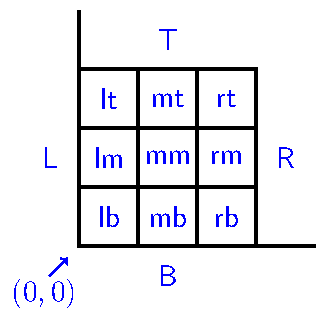
\includegraphics[height=3cm]{rubik-doc-figD.pdf}
%  \fi
%  \vspace{-5mm}
%   \caption{\label{fig:facenotation}Face-edge and facelet-position codes 
%                       (see text) } 
%  \end{figure}
% 
%
% \begin{macro}{\side@barT}
% \begin{macro}{\side@barB}
% \begin{macro}{\side@barL}
% \begin{macro}{\side@barR}
% There are four \cmd{\side@barX} commands, each with a trailing letter code X, which indicates the 
% position of the sidebar relative to the square face displayed, 
% namely  either T (Top), B (Bottom), L (Left) or R (Right) 
% ---see Figure~\ref{fig:facenotation}. 

% \cmd{\side@barL}\marg{position-number}\marg{facelet location-code}.
% Each \cmd{\side@barX} command  takes two arguments:
% The first argument is a number (distance)   \marg{$ 1 \mid 2 \mid 3$}
% from the relevant axis depending on whether  it is a vertical or horizontal sidebar 
% (e.g.,~1 = first bar (nearest the origin); 2 = second bar, 
% 3 = third bar). 
%
% The second argument is the facelet location-code  expressed as a command 
%   (e.g.,~\cmd{\Lrt}, \cmd{\Dlb} etc. Note that the  facelet location 
% uses a three letter code: the first (capital) letter (U, D, L, R, F, B) denotes the \textsc{face};
% the second (lower-case) letter (l,m,r) is the `x' position in the 3x3 matrix;
% the third (lower-case) letter (t,m,b) is the `y' position ---see Figure~\ref{fig:facenotation}.  
%
% \textsc{example}: the following command draws a small single Right sidebar, 
% in the middle position (no.~2),  with the colour 
% allocated to the Rlt facelet (left top facelet in the \textsc{right} face. 
%  \begin{quote}
%     \verb!\side@barR{2}{\Rlt}!
%  \end{quote}
% Notice that we use the command \cmd{\Rlt}  as the argument; this is because 
% the command is defined as: \verb!\def{\Rlt}{#1}!, and hence the command gets replaced by the
%  colour-code currently allocated to  this particular facelet.
%
% There are three small rectangular sidebars on  each of the four sides 
% of a 3x3 square face, and these are embedded in a coordinate system with origin
% at the bottom left corner (0,0) of the square face (see Figure~\ref{fig:facenotation}).
% 
% The \cmd{\side@bar..} command  also implements the set (or default) 
% RubikSidebarLength \cmd{\bl}, RubikSidebarWidth \cmd{\bw} 
% and RubikSidebarSep \cmd{\bs} (separation) 
% values mentioned above. \cmd{\blh} = Half \cmd{\bl} = \cmd{\bl}/2.
% Note that the TikZ \cmd{\pgfmathsetmacro} commands (which do the maths)
%  must be inside  the  \cmd{\side@bar..} command in order to work.
% The start point of the TikZ \cmd{\draw} command for  each  rectangular sidebar 
%    is the bottom Left corner of the sidebar = (\cmd{\dx},\cmd{\dy}).
% \end{macro}
% \end{macro}
% \end{macro}
% \end{macro}
%
%
%  \label{sec:nosidebarcode}
%    \begin{macro}{\no@sidebar}
% The \cmd{\NoSidebar}\marg{colour code} command defines a (single) colour for which
% sidebars should  \textit{not} be drawn (particularly useful when drawing OLL configurations).  
% This idea was suggested by Robert Ma\v{r}\'{\i}k (May 2017) ---see Section~\ref{sec:nosidebar}.
% {\newline}The principle is that we let the command \cmd{\NoSidebar} define a face colour,
% and then we use the \verb!\ifthenelse{\equal{#2}{\no@sidebar}}{}{...}! structure 
% inside the \cmd{\side@bar..} commands (see below)
% to either (a)~draw all sidebars as usual (if \cmd{\NoSidebar} is undefined), 
% or (b)~draw all sidebars \textit{except}
% those having the \cmd{\NoSidebar} colour (if \cmd{\NoSidebar} colour = \verb!#2!). 
% \newline\textsc{usage}: \verb!\NoSidebar{X}! \  If this command in \textit{not} 
% inside an environment, then its action will continue until it is disabled 
% (undefined) as follows: \verb!\NoSidebar{}!.
%    \begin{macrocode}
\def\no@sidebar{}%
\newcommand{\NoSidebar}[1]{\def\no@sidebar{#1}}
%    \end{macrocode}
%    \end{macro}
%
%
%    \begin{macrocode}
\newcommand{\side@barL}[2]{%
  %% #1 = cubie possn no, #2 = colour
  \ifthenelse{\equal{#2}{\no@sidebar}}{}{%
  \pgfmathsetmacro{\blh}{\bl*(0.5)}%
  \pgfmathsetmacro{\dx}{0 - \bs - \bw}%
  \pgfmathsetmacro{\dy}{#1-1+0.5-\blh}%
  \draw[fill=#2] (\dx,\dy) -- (\dx,\dy + \bl) 
  -- (\dx+\bw,\dy+\bl) -- (\dx+\bw,\dy) -- cycle;
}}
\newcommand{\side@barR}[2]{%
  %% #1 = cubie possn no, #2 = colour
  \ifthenelse{\equal{#2}{\no@sidebar}}{}{%
  \pgfmathsetmacro{\blh}{\bl*(0.5)}%
  \pgfmathsetmacro{\dx}{3 + \bs}%
  \pgfmathsetmacro{\dy}{#1 -1+0.5-\blh}%
  \draw[fill=#2] (\dx,\dy) -- (\dx,\dy + \bl)
  -- (\dx+\bw,\dy+\bl) -- (\dx+\bw,\dy) -- cycle;
}}
\newcommand{\side@barT}[2]{%
  %% #1 = cubie possn no, #2 = colour
  \ifthenelse{\equal{#2}{\no@sidebar}}{}{%
  \pgfmathsetmacro{\blh}{\bl*(0.5)}%
  \pgfmathsetmacro{\dx}{#1 -1+0.5-\blh}%
  \pgfmathsetmacro{\dy}{3 +\bs}%
  \draw[fill=#2] (\dx,\dy) -- (\dx,\dy + \bw)
  -- (\dx+\bl,\dy+\bw) -- (\dx+\bl,\dy) -- cycle;
}}
\newcommand{\side@barB}[2]{%
  %% #1 = cubie possn no, #2 = colour
  \ifthenelse{\equal{#2}{\no@sidebar}}{}{%
  \pgfmathsetmacro{\blh}{\bl*(0.5)}%
  \pgfmathsetmacro{\dx}{#1 -1+0.5-\blh}%
  \pgfmathsetmacro{\dy}{0 -\bs-\bw}%
  \draw[fill=#2] (\dx,\dy) -- (\dx,\dy + \bw)
  -- (\dx+\bl,\dy+\bw) -- (\dx+\bl,\dy) -- cycle;
}}
%    \end{macrocode}
%
% RWDN19C  removed 20:17:2 and 20:17:3 19 Feb 2018
%
%
%
%
%
%
% \subsection{Sidebars (Cube)}
%  \label{sec:sidebarscubecode}
%
%
% In order to position sidebars adjacent to a Rubik Cube (ie in 3D) 
% requires that we first make  some  new  \cmd{\side@bar..}
% commands for drawing sidebars adjacent to the \textsc{back} face of the cube
% (we have already made the macros for the front 
% face sidebars---see Section~\ref{sec:sidebarcode}).
% Furthermore, these new macros need to be tailored  to each of the 
% four standard cube  viewing directions RU, LU, RD, LD.
%
% Finally, the USER commands for drawing these sidebars need 
% to accommodate (a)~some code for identifying each set of sidebars, 
% and (b)~the viewing direction. So, for example,  a USER command for 
% drawing  the sidebars associated with the cube edge formed 
% by the \textsc{right} face and the \textsc{back} face 
% (lets define this as the RB sidebar) as viewed from the RU direction, 
% might be something like \cmd{\DrawRubikCubeSidebarRBRU}. 
% Since this is not particularly user-friendly, 
% we can improve on this slightly for the USER by 
% (a)~defining the sidebar as \texttt{SidebarRB}, and 
% (b)~appending the view direction in a curly bracket, say as \verb!{RU}!. 
% This allows a more intuitive command structure for the USER, 
%  as follows: \verb!\DrawRubikCubeSidebarRB{RU}!.
% We then use the \cmd{\@join} command to append the string \verb!RU! to the string 
% \verb!DrawRubicCubeSidebarRB! forming the (internal) 
% command \cmd{\DrawRubicCubeSidebarRBRU}.
%
% In the following we will group the code according to to the view 
% direction (RU, LU, RD, LD).
%
%
%
%  \subsubsection{Sidebars: RU view}
%
%  \subsubsection*{Right-Back vert sidebar (RU view)}
%
%
% Need to write a new command for this position
% modified from \cmd{\side@barR} (in Section 20.16.1)
% draws only a single small bar 
% each of the three  small bars has a numbered position (1,2,3);
% (dx,dy) = bottom Left corner of single facelet bar
%    \begin{macrocode}
\newcommand{\side@barRubikRbackRU}[2]{%
  %% #1 = cubie possn no, #2 = colour
  %% dx --> dx+1
  %% dy --> dy+1
  \ifthenelse{\equal{#2}{\no@sidebar}}{}{%
  \pgfmathsetmacro{\blh}{\bl*(0.5)}%
  \pgfmathsetmacro{\dx}{3 + \bs +1}%
  \pgfmathsetmacro{\dy}{#1 -1+0.5-\blh +1}%
  \draw[fill=#2] (\dx,\dy) -- (\dx,\dy + \bl)
  -- (\dx+\bw,\dy+\bl) -- (\dx+\bw,\dy) -- cycle;
}}
%    \end{macrocode}
% Make the RB (RightBack) version;
% bar 1 is at the bottom
%    \begin{macrocode}
\newcommand{\DrawRubikCubeSidebarRBRU}{%
\side@barRubikRbackRU{3}{\Blt}%
\side@barRubikRbackRU{2}{\Blm}%
\side@barRubikRbackRU{1}{\Blb}%
}
%    \end{macrocode}
% Now do the reverse (BR) = RB
%    \begin{macrocode}
\newcommand{\DrawRubikCubeSidebarBRRU}{\DrawRubikCubeSidebarRBRU}
%    \end{macrocode}
% Make the join commands
%    \begin{macrocode}
\newcommand{\DrawRubikCubeSidebarRB}[1]{\@join{\DrawRubikCubeSidebarRB}{#1}}
\newcommand{\DrawRubikCubeSidebarBR}[1]{\@join{\DrawRubikCubeSidebarBR}{#1}}
%    \end{macrocode}
%
%
%  \medskip
%
%  \subsubsection*{Up-Back horiz sidebar (RU view)}
%
%
% Need to write a new command for this position
% modified from \cmd{\side@barT} (in Section 20.16.1)
% draws only a single small bar 
% each of the three small bars has a numbered position (1,2,3);
% (dx,dy) = bottom Left corner of single facelet bar
%    \begin{macrocode}
\newcommand{\side@barRubikTbackRU}[2]{%
  %% #1 = cubie possn no; #2 = colour
  %% dx --> dx+1
  %% dy --> dy+1
  \ifthenelse{\equal{#2}{\no@sidebar}}{}{%
  \pgfmathsetmacro{\blh}{\bl*(0.5)}%
  \pgfmathsetmacro{\dx}{#1 -1+0.5-\blh +1}%
  \pgfmathsetmacro{\dy}{3 +\bs +1}%
  \draw[fill=#2] (\dx,\dy) -- (\dx,\dy + \bw)
  -- (\dx+\bl,\dy+\bw) -- (\dx+\bl,\dy) -- cycle;
}}
%    \end{macrocode}
% Make the UB (Up-Back) version;
% bar 1 is at the left, 3 on the rhs (as we look at the image)
%    \begin{macrocode}
\newcommand{\DrawRubikCubeSidebarUBRU}{%
\side@barRubikTbackRU{1}{\Brt}%
\side@barRubikTbackRU{2}{\Bmt}%
\side@barRubikTbackRU{3}{\Blt}%
}
%    \end{macrocode}
% Now do the reverse (BU) = UB
%    \begin{macrocode}
\newcommand{\DrawRubikCubeSidebarBURU}{\DrawRubikCubeSidebarUBRU}
%    \end{macrocode}
% Make the join commands
%    \begin{macrocode}
\newcommand{\DrawRubikCubeSidebarUB}[1]{\@join{\DrawRubikCubeSidebarUB}{#1}}
\newcommand{\DrawRubikCubeSidebarBU}[1]{\@join{\DrawRubikCubeSidebarBU}{#1}}
%    \end{macrocode}
%
%
% \medskip
%
%  \subsubsection*{Front-Left vert sidebar (RU view)}
%
% For the front face we can use the regular \cmd{side@barL} commands 
% since it is the same as for an ordinary face sidebar
%    \begin{macrocode}
\newcommand{\DrawRubikCubeSidebarFLRU}{%
\side@barL{3}{\Lrt}%
\side@barL{2}{\Lrm}%
\side@barL{1}{\Lrb}%
}
%    \end{macrocode}
% Now do the reverse (LF)
%    \begin{macrocode}
\newcommand{\DrawRubikCubeSidebarLFRU}{\DrawRubikCubeSidebarFLRU}
%    \end{macrocode}
% Now do the two join commands
%    \begin{macrocode}
\newcommand{\DrawRubikCubeSidebarFL}[1]{\@join{\DrawRubikCubeSidebarFL}{#1}}
\newcommand{\DrawRubikCubeSidebarLF}[1]{\@join{\DrawRubikCubeSidebarLF}{#1}}
%    \end{macrocode}
%
%
%  \medskip
%
%  \subsubsection*{Front-Down horizontal sidebar (RU view)}
%
% Horiz sidebar, so 1 at the left, 2=middle, 3= rhs)
% here we have to use the B for bottom (of front face) and the 
% facelets of the  top row of the Down face
%    \begin{macrocode}
\newcommand{\DrawRubikCubeSidebarFDRU}{%
\side@barB{1}{\Dlt}%
\side@barB{2}{\Dmt}%
\side@barB{3}{\Drt}%
}
%    \end{macrocode}
% Now do the reverse (DF) = FD
%    \begin{macrocode}
\newcommand{\DrawRubikCubeSidebarDFRU}{\DrawRubikCubeSidebarFDRU}
%    \end{macrocode}
% Now do the two join commands
%    \begin{macrocode}
\newcommand{\DrawRubikCubeSidebarFD}[1]{\@join{\DrawRubikCubeSidebarFD}{#1}}
\newcommand{\DrawRubikCubeSidebarDF}[1]{\@join{\DrawRubikCubeSidebarDF}{#1}}
%    \end{macrocode}
% But FD-LU  is the same as FD-RU, so need to make copies of each
%    \begin{macrocode}
\newcommand{\DrawRubikCubeSidebarDFLU}{\DrawRubikCubeSidebarDFRU}
\newcommand{\DrawRubikCubeSidebarFDLU}{\DrawRubikCubeSidebarFDRU}
%    \end{macrocode}
%
%
%  \medskip
%
%  \subsubsection{Sidebars: LU view}
%
%
%  \subsubsection*{Left-Back vert sidebar (LU view)}
%
% Need to write a new command for this position
% modified from \cmd{\side@barL} (in Section 20.16.1)
% draws only a single small bar 
% each of the three  small bars has a numbered position (1,2,3);
% (dx,dy) = bottom Left corner of single facelet bar
%    \begin{macrocode}
\newcommand{\side@barRubikLbackLU}[2]{%
  %% #1 = cubie possn no, #2 = colour
  %% dx --> dx-1
  %% dy --> dy+1
  \ifthenelse{\equal{#2}{\no@sidebar}}{}{%
  \pgfmathsetmacro{\blh}{\bl*(0.5)}%
  \pgfmathsetmacro{\dx}{0 - \bs -\bw -1}%
  \pgfmathsetmacro{\dy}{#1 -1+0.5-\blh +1}%
  \draw[fill=#2] (\dx,\dy) -- (\dx,\dy + \bl)
  -- (\dx+\bw,\dy+\bl) -- (\dx+\bw,\dy) -- cycle;
}}
%    \end{macrocode}
% Make the LB (LeftBack) version;
% bar 1 is at the bottom
%    \begin{macrocode}
\newcommand{\DrawRubikCubeSidebarLBLU}{%
\side@barRubikLbackLU{3}{\Brt}%
\side@barRubikLbackLU{2}{\Brm}%
\side@barRubikLbackLU{1}{\Brb}%
}
%    \end{macrocode}
% Now do the reverse (BL) = LB
%    \begin{macrocode}
\newcommand{\DrawRubikCubeSidebarBLLU}{\DrawRubikCubeSidebarLBLU}
%    \end{macrocode}
% Make the join commands
%    \begin{macrocode}
\newcommand{\DrawRubikCubeSidebarLB}[1]{\@join{\DrawRubikCubeSidebarLB}{#1}}
\newcommand{\DrawRubikCubeSidebarBL}[1]{\@join{\DrawRubikCubeSidebarBL}{#1}}
%    \end{macrocode}
%
%
% \medskip
%
%  \subsubsection*{Up-Back horizontal sidebar (LU view)}
%
% Modified from \cmd{\side@barT} (in Section 20.16.1)
% draws only a single small bar 
% each of the three  small bars has a numbered position (1,2,3);
% (dx,dy) = bottom Left corner of single facelet bar
%    \begin{macrocode}
\newcommand{\side@barRubikTbackLU}[2]{%
  %% #1 = cubie possn no; #2 = colour
  %% dx --> dx-1
  %% dy --> dy+1
  \ifthenelse{\equal{#2}{\no@sidebar}}{}{%
  \pgfmathsetmacro{\blh}{\bl*(0.5)}%
  \pgfmathsetmacro{\dx}{#1 -1+0.5-\blh -1}%
  \pgfmathsetmacro{\dy}{3 +\bs +1}%
  \draw[fill=#2] (\dx,\dy) -- (\dx,\dy + \bw)
  -- (\dx+\bl,\dy+\bw) -- (\dx+\bl,\dy) -- cycle;
}}
%    \end{macrocode}
% Make the UB (Up-Back) version;
% bar 1 is at the left, 3 on the rhs (as we look at the image)
%    \begin{macrocode}
\newcommand{\DrawRubikCubeSidebarUBLU}{%
\side@barRubikTbackLU{1}{\Brt}%
\side@barRubikTbackLU{2}{\Bmt}%
\side@barRubikTbackLU{3}{\Blt}%
}
%    \end{macrocode}
% Now do the reverse (BU) = UB
%    \begin{macrocode}
\newcommand{\DrawRubikCubeSidebarBULU}{\DrawRubikCubeSidebarUBLU}
%    \end{macrocode}
% Do not need to make the join commands
% as the USER commands for  BU and UB are the same as for the RU.
%
%
% \medskip
%
%  \subsubsection*{Front-Right vertical sidebar (LU view)}
%
% Only needed for the LU view and LD.
% for the front face we can use the regular side@barR commands 
% since it is the same as for an ordinary face sidebar RHS
%    \begin{macrocode}
\newcommand{\DrawRubikCubeSidebarFRLU}{%
\side@barR{3}{\Rlt}%
\side@barR{2}{\Rlm}%
\side@barR{1}{\Rlb}%
}
%    \end{macrocode}
% Now do the reverse (RF)
%    \begin{macrocode}
\newcommand{\DrawRubikCubeSidebarRFLU}{\DrawRubikCubeSidebarFRLU}
%    \end{macrocode}
% Now do the two join commands
%    \begin{macrocode}
\newcommand{\DrawRubikCubeSidebarFR}[1]{\@join{\DrawRubikCubeSidebarFR}{#1}}
\newcommand{\DrawRubikCubeSidebarRF}[1]{\@join{\DrawRubikCubeSidebarRF}{#1}}
%    \end{macrocode}
%
%
%
%
%  \subsubsection{Sidebars: RD view}
%
% \medskip
%
%  \subsubsection*{Front-Up horizontal sidebar (RD view)}
%
% Horiz sidebar, so 1 at the left, 2=middle, 3= rhs
% here we have to use the T for bottom (of front face) and the 
% facelets of the  top row of the Down face
%    \begin{macrocode}
\newcommand{\DrawRubikCubeSidebarFURD}{%
\side@barT{1}{\Ulb}%
\side@barT{2}{\Umb}%
\side@barT{3}{\Urb}%
}
%    \end{macrocode}
% Now do the reverse (UF) = FU
%    \begin{macrocode}
\newcommand{\DrawRubikCubeSidebarUFRD}{\DrawRubikCubeSidebarFURD}
%    \end{macrocode}
% Now do the two join commands
%    \begin{macrocode}
\newcommand{\DrawRubikCubeSidebarFU}[1]{\@join{\DrawRubikCubeSidebarFU}{#1}}
\newcommand{\DrawRubikCubeSidebarUF}[1]{\@join{\DrawRubikCubeSidebarUF}{#1}}
%    \end{macrocode}
%
% \medskip
%
%  \subsubsection*{Front-Left vertical sidebar (RD view)}
%
%
%
% Front LEFT (RD view = same as for RU)
%    \begin{macrocode}
\newcommand{\DrawRubikCubeSidebarFLRD}{\DrawRubikCubeSidebarFLRU}
\newcommand{\DrawRubikCubeSidebarLFRD}{\DrawRubikCubeSidebarLFRU}
%    \end{macrocode}
%
%
% \medskip
%
%  \subsubsection*{Right-Back vertical sidebar (RD view)}
%
% Modified from \cmd{\side@barR} (in Section 20.16.1)
% draws only a single small bar 
% each of the three  small bars has a numbered position (1,2,3);
% (dx,dy) = bottom Left corner of single facelet bar
%    \begin{macrocode}
\newcommand{\side@barRubikRbackRD}[2]{%
  %% #1 = cubie possn no, #2 = colour
  %% dx --> dx+1
  %% dy --> dy-1
  \ifthenelse{\equal{#2}{\no@sidebar}}{}{%
  \pgfmathsetmacro{\blh}{\bl*(0.5)}%
  \pgfmathsetmacro{\dx}{3 + \bs +1}%
  \pgfmathsetmacro{\dy}{#1 -1+0.5-\blh -1}%
  \draw[fill=#2] (\dx,\dy) -- (\dx,\dy + \bl)
  -- (\dx+\bw,\dy+\bl) -- (\dx+\bw,\dy) -- cycle;
}}
%    \end{macrocode}
% Make the RB (RightBack) version;
% bar 1 is at the bottom
%    \begin{macrocode}
\newcommand{\DrawRubikCubeSidebarRBRD}{%
\side@barRubikRbackRD{3}{\Blt}%
\side@barRubikRbackRD{2}{\Blm}%
\side@barRubikRbackRD{1}{\Blb}%
}
%    \end{macrocode}
% Now do the reverse (BR) = RB
%    \begin{macrocode}
\newcommand{\DrawRubikCubeSidebarBRRD}{\DrawRubikCubeSidebarRBRD}
%    \end{macrocode}
% Do NOT need to make the join commands (same as for the RU view)
%
%
% \medskip
%
%  \subsubsection*{Down-Back horizotal sidebar (RD view)}
%
% Modified from \cmd{\side@barB} (in Section 20.16.1)
% draws only a single small bar 
% each of the three small bars has a numbered position (1,2,3);
% (dx,dy) = bottom Left corner of single facelet bar
%    \begin{macrocode}
\newcommand{\side@barRubikBbackRD}[2]{%
  %% #1 = cubie possn no; #2 = colour
  %% dx --> dx+1
  %% dy --> dy-1
  \ifthenelse{\equal{#2}{\no@sidebar}}{}{%
  \pgfmathsetmacro{\blh}{\bl*(0.5)}%
  \pgfmathsetmacro{\dx}{#1 -1+0.5-\blh +1}%
  \pgfmathsetmacro{\dy}{0 -\bs - \bw -1}%
  \draw[fill=#2] (\dx,\dy) -- (\dx,\dy + \bw)
  -- (\dx+\bl,\dy+\bw) -- (\dx+\bl,\dy) -- cycle;
}}
%    \end{macrocode}
% Make the DB (Down-Back) version;
% bar 1 is at the left, 3 on the rhs (as we look at the image) 
%    \begin{macrocode}
\newcommand{\DrawRubikCubeSidebarDBRD}{%
\side@barRubikBbackRD{1}{\Brb}%
\side@barRubikBbackRD{2}{\Bmb}%
\side@barRubikBbackRD{3}{\Blb}%
}
%    \end{macrocode}
% Now do the reverse (BD) = DB
%    \begin{macrocode}
\newcommand{\DrawRubikCubeSidebarBDRD}{\DrawRubikCubeSidebarDBRD}
%    \end{macrocode}
% Make the join commands
%    \begin{macrocode}
\newcommand{\DrawRubikCubeSidebarDB}[1]{\@join{\DrawRubikCubeSidebarDB}{#1}}
\newcommand{\DrawRubikCubeSidebarBD}[1]{\@join{\DrawRubikCubeSidebarBD}{#1}}
%    \end{macrocode}
%
%
%
%  \subsubsection{Sidebars: LD  view}
%
%
% \medskip
%
%  \subsubsection*{Front-Up horizontal sidebar (LD view)}
%
% But FR (LD view) is the same as for (RU view), (see above)
%    \begin{macrocode}
\newcommand{\DrawRubikCubeSidebarFULD}{\DrawRubikCubeSidebarFURD}
\newcommand{\DrawRubikCubeSidebarUFLD}{\DrawRubikCubeSidebarUFRD}
%    \end{macrocode}
%
% \medskip
%
%  \subsubsection*{Front-Right vertical sidebar (LD view)}
%
% Front Right (LDview) = same as for (LU view),  (see above)
%    \begin{macrocode}
\newcommand{\DrawRubikCubeSidebarFRLD}{\DrawRubikCubeSidebarFRLU}
\newcommand{\DrawRubikCubeSidebarRFLD}{\DrawRubikCubeSidebarRFLU}
%    \end{macrocode}
%
%
% \medskip
%
%  \subsubsection*{Left-Back vertical sidebar (LD view)}
%
% Modified from \cmd{\side@barL} (in Section 20.16.1)
% draws only a single small bar 
% each of the three small bars has a numbered position (1,2,3);
% (dx,dy) = bottom Left corner of single facelet bar
%    \begin{macrocode}
\newcommand{\side@barRubikLbackLD}[2]{%
  %% #1 = cubie possn no, #2 = colour
  %% dx --> dx-1
  %% dy --> dy-1
  \ifthenelse{\equal{#2}{\no@sidebar}}{}{%
  \pgfmathsetmacro{\blh}{\bl*(0.5)}%
  \pgfmathsetmacro{\dx}{0 - \bs -\bw -1}%
  \pgfmathsetmacro{\dy}{#1 -1+0.5-\blh -1}%
  \draw[fill=#2] (\dx,\dy) -- (\dx,\dy + \bl)
  -- (\dx+\bw,\dy+\bl) -- (\dx+\bw,\dy) -- cycle;
}}
%    \end{macrocode}
% Make the LB (LeftBack) version;
% bar 1 is at the bottom
%    \begin{macrocode}
\newcommand{\DrawRubikCubeSidebarLBLD}{%
\side@barRubikLbackLD{3}{\Brt}%
\side@barRubikLbackLD{2}{\Brm}%
\side@barRubikLbackLD{1}{\Brb}%
}
%    \end{macrocode}
% Now do the reverse (BL) = LB
%    \begin{macrocode}
\newcommand{\DrawRubikCubeSidebarBLLD}{\DrawRubikCubeSidebarLBLD}
%    \end{macrocode}
% Do NOT need to make the join commands (same as for the LU view)
%
%
% \medskip
%
%  \subsubsection*{Down-Back horizontal sidebar (LD view)}
%
%
% Modified from \cmd{\side@barB} (in Section 20.16.1)
% draws only a single small bar 
% each of the three  small bars has a numbered position (1,2,3);
% (dx,dy) = bottom Left corner of single facelet bar
%    \begin{macrocode}
\newcommand{\side@barRubikBbackLD}[2]{%
  %% #1 = cubie possn no; #2 = colour
  %% dx --> dx-1
  %% dy --> dy-1
  \ifthenelse{\equal{#2}{\no@sidebar}}{}{%
  \pgfmathsetmacro{\blh}{\bl*(0.5)}%
  \pgfmathsetmacro{\dx}{#1 -1+0.5-\blh -1}%
  \pgfmathsetmacro{\dy}{0 -\bs - \bw -1}%
  \draw[fill=#2] (\dx,\dy) -- (\dx,\dy + \bw)
  -- (\dx+\bl,\dy+\bw) -- (\dx+\bl,\dy) -- cycle;
}}
%    \end{macrocode}
% Make the DB (Down-Back) version;
% bar 1 is at the left, 3 on the rhs (as we look at the image)
%    \begin{macrocode}
\newcommand{\DrawRubikCubeSidebarDBLD}{%
\side@barRubikBbackLD{1}{\Brb}%
\side@barRubikBbackLD{2}{\Bmb}%
\side@barRubikBbackLD{3}{\Blb}%
}
%    \end{macrocode}
% Now do the reverse (BD) = DB
%    \begin{macrocode}
\newcommand{\DrawRubikCubeSidebarBDLD}{\DrawRubikCubeSidebarDBLD}
%    \end{macrocode}
% Do NOT need to make the join commands (same as for the RD view
%
%
%
%
%    \subsection{\hspace{3mm}DrawNCube command}
%
%  \textsc{history}: The essence of this command was originally developed by Peter Bartal 
%  as his command \cmd{\rubikcube} (see Bartal,
%  2011). We have modified it, as follows (June 2012):
%  \newline\strut\hspace{\parindent}(1) adjusted  to use the 
%  TikZ \cmd{\pgfmathsetmacro\{\}\{\}} command (suggested by Peter Grill),
%  \newline\strut\hspace{\parindent}(2)  renamed to \cmd{\DrawNCubeAll}.
%
%    \begin{macro}{\DrawNCubeAll}
% {\noindent}This command draws a solved NxNxN Rubik's cube from the RightUp viewpoint.
% All cubies on a given face have the same colour. 
% The command takes four ordered  arguments, as follows:
% \begin{quote}
%   \#1 = number of cubies ($n>0$) along each side,
%   {\newline}\#2, \#3, \#4 = colours of the visible faces (in X,Y,Z order);
%             X=Right face  colour, Y=Up face colour, Z=Front face colour.
% \end{quote}
% We use the  \cmd{\pgfmathsetmacro}\marg{variable-name}\marg{numeric value or maths}
% command. Note that the second argument must not involve any units---just numeric 
% values or mathematics.
%
% \begin{macrocode}
\newcommand{\DrawNCubeAll}[4]{%
   \pgfmathsetmacro{\ncubes}{#1-1}%
%% need to subtract 1 from the given number of cubies per side 
%% to avoid the origin of the initial cube to be displaced
    \foreach \x in {0,...,\ncubes}{%
      \foreach \y in {0,...,\ncubes}{%
        \foreach \z in {0,...,\ncubes}{%
          \cube@dxdydz{1}{#2}{#3}{#4}{\x}{\y}{\z}% 
  }}}}
%    \end{macrocode}
%    \end{macro}
%
%   \begin{macro}{\cube@dxdydz}
% This internal command is  used only by the \cmd{\DrawNCubeAll} command 
% (see above).  The original version of this command was developed  
% by Peter Bartal (see Bartal, 2011).
% It was later modified (2012) by RWD Nickalls (to implement  a more 
% intuitive X, Y, Z ordering of the face colour parameters).
%
%  The cube need not be in the origin, the distances of 
% the \textsc{down}-behind [L] corner from 
% the origin are taken as parameters 5,6,7.
% The command takes 7 ordered arguments:
% \begin{quote}
% 1 - length of an edge 
% {\newline}2 - X-face colour (\textsc{right} face)
% {\newline}3 - Y-face colour (\textsc{up} face)
% {\newline}4 - Z-face colour (\textsc{front} face)
% {\newline}5 - x-position in space
% {\newline}6 - y-position in space
% {\newline}7 - z-position in space
% \end{quote}
%
% \textsc{usage}:  |\cube@dxdydz{1}{X}{Y}{Z}{x}{y}{z}|
%
% {\noindent}The original code
%   |\pgfmathparse{#1+#5}\let\dy\pgfmathresult| 
% {\newline} was changed  to the more intuitive  |\pgfmathsetmacro{\dx}{#1+#5}|
% (suggested by Peter Grill 2011).
%
% \textsc{changes}: RWD Nickalls (2012): 
% (1) added the [line join=round,line cap=round] 
% options to  each of the TikZ  \cmd{\draw} commands, in order to improve 
% the line joining (first two options); (2) adjusted  the \cmd{\cube@dxdydz} macro 
% to adopt the ordered  XYZ face colour notation
% (by reassigning \#2, \#3, \#4  to the X, Y, Z face colours, as shown above).
%
%    \begin{macrocode}
\newcommand{\cube@dxdydz}[7]{%
   \pgfmathsetmacro{\dx}{#1+#5}% 
%% calculates the 'displacement' (distance from the origin) of the 
%% far corners of the cube along the x axis from the arguments
   \pgfmathsetmacro{\dy}{#1+#6}%
%% calculates the 'displacement' (distance from the origin) of the 
%% far corners of the cube along the y axis from the arguments
   \pgfmathsetmacro{\dz}{#1+#7}%
%% calculates the 'displacement' (distance from the origin) of the 
%% far corners of the cube along the z axis from the arguments
%% Draw FRONT face   (using the X colour = #4)
    \draw[line join=round,line cap=round,ultra thick,fill=#4]%
 (#5,#6,\dz) -- (\dx,#6,\dz) -- (\dx,\dy,\dz) -- (#5,\dy,\dz) -- cycle;
%% The 'rectangle' command does not work with 3D coordinates, 
%% so this is the way to draw the squares with space coordinates
%% Draw UP face (using the Y colour = #3)
   \draw[line join=round,line cap=round,ultra thick,fill=#3]%
 (#5,\dy,\dz) -- (\dx,\dy,\dz) -- (\dx,\dy,#7) -- (#5,\dy,#7) -- cycle;
%% Draw RIGHT face   (using the X colour = #2)
 \draw[line join=round,line cap=round,ultra thick,fill=#2]%
 (\dx,#6,\dz) -- (\dx,#6,#7) -- (\dx,\dy,#7) -- (\dx,\dy,\dz) -- cycle;
    }
%    \end{macrocode}
%    \end{macro}
%
%
%
%  \subsection{\hspace{3mm}Drawing single cubies}
%
%  \begin{macro}{\Cubiedx}
%  \begin{macro}{\Cubiedy}
%  These two commands set the value of the two length parameters
%  \texttt{cx} and \texttt{cy}, and allow the user to vary the size 
%  (adjust \texttt{cy}) and horizontal viewpoint  (adjust \texttt{cx})
%  of a single cubie (described in more detail in the \rubikcube\ 
%   package  documentation).
%  Note that we cannot use the names \texttt{dx}, \texttt{dy} for the 
%  variables here since  these names have been  allocated already 
%  (see above). However, we can  use  \texttt{dx}, \texttt{dy} in the  
%  command names  as these will be more  readily understood by the user.
%    \begin{macrocode}
\newcommand{\Cubiedx}[1]{\pgfmathsetmacro{\cx}{#1}}
\newcommand{\Cubiedy}[1]{\pgfmathsetmacro{\cy}{#1}}
%    \end{macrocode}
%    \end{macro}
%    \end{macro}
% We now set the default values (cx=cy=0.4)
%    \begin{macrocode}
\Cubiedx{0.4}
\Cubiedy{0.4}
%    \end{macrocode}
%
%
%  \begin{macro}{\DrawCubieRU}
%  \begin{macro}{\DrawCubieRD}
%  \begin{macro}{\DrawCubieLU}
%  \begin{macro}{\DrawCubieLD}
% These four commands draw a single cubie from the RightUp, RightDown, 
% LeftUp, LeftDown viewpoint. The viewpoint is specified using an appended 
% two-letter XY ordered viewpoint code: either RU, RD, LU, LD.
% These commands take three arguments, namely three different XYZ 
% ordered colour codes (R,O,Y,G,B,W,X).
% \newline\textsc{format}: \cmd{\DrawCubieRU}\marg{Xcolour}\marg{Ycolour}\marg{Zcolour}
% \newline\textsc{usage}: |\DrawCubieRU{G}{B}{W}|
%    \end{macro}
%    \end{macro}
%    \end{macro}
%    \end{macro}
%    \begin{macrocode}
\newcommand{\DrawCubieRU}[3]{%
%% Front face (z)
\draw[line join=round,line cap=round,ultra thick,fill=#3]%
 (0,0) -- (0, 1) -- (1, 1) -- (1,0) -- cycle;
%% Up face(y)
\draw[line join=round,line cap=round,ultra thick,fill=#2]%
 (0,1) -- (\cx, 1+\cy) -- (1+\cx,1+\cy) -- (1,1) -- cycle;
%% Right face(x)
\draw[line join=round,line cap=round,ultra thick,fill=#1]%
 (1,0) -- (1,1) -- (1+\cx,1+\cy) -- (1+\cx, \cy) -- cycle;
}
\newcommand{\DrawCubieRD}[3]{%
%% Front face (z)
\draw[line join=round,line cap=round,ultra thick,fill=#3]%
 (0,0) -- (0, 1) -- (1, 1) -- (1,0) -- cycle;
%% Down face (y)
\draw[line join=round,line cap=round,ultra thick,fill=#2]%
 (\cx,-\cy) -- (0, 0) -- (1,0) -- (1+\cx,-\cy) -- cycle;
%% Right face (x)
\draw[line join=round,line cap=round,ultra thick,fill=#1]%
 (1,0) -- (1,1) -- (1+\cx,-\cy+1) -- (1+\cx, -\cy) -- cycle;
}
\newcommand{\DrawCubieLD}[3]{%
%% Front face (z)
\draw[line join=round,line cap=round,ultra thick,fill=#3]%
 (0,0) -- (0, 1) -- (1, 1) -- (1,0) -- cycle;
%% Down face (y)
\draw[line join=round,line cap=round,ultra thick,fill=#2]%
 (-\cx,-\cy) -- (0, 0) -- (1,0) -- (1-\cx,-\cy) -- cycle;
%% Left face (x)
\draw[line join=round,line cap=round,ultra thick,fill=#1]%
 (-\cx,-\cy) -- (-\cx,-\cy+1) -- (0,1) -- (0,0) -- cycle;
}
\newcommand{\DrawCubieLU}[3]{%
%% Front face (z)
\draw[line join=round,line cap=round,ultra thick,fill=#3]%
 (0,0) -- (0, 1) -- (1, 1) -- (1,0) -- cycle;
%% Up face (y)
\draw[line join=round,line cap=round,ultra thick,fill=#2]%
 (-\cx,1+\cy) -- (1-\cx, 1+\cy) -- (1,1) -- (0,1) -- cycle;
%% Left face (x)
\draw[line join=round,line cap=round,ultra thick,fill=#1]%
 (-\cx, \cy) -- (-\cx,\cy+1) -- (0,1) -- (0,0) -- cycle;
}
%    \end{macrocode}
%
%
%  \subsection{\hspace{3mm}Text cubies}
% 
%  \begin{macro}{\textCubieRU}
%  \begin{macro}{\textCubieRD}
%  \begin{macro}{\textCubieLU}
%  \begin{macro}{\textCubieLD}
%  These four commands draw a single `text' cubie from the RightUp, RightDown, 
%  LeftUp, LeftDown viewpoint. 
%  They are `text' forms of the \cmd{\DrawCubie} commands described above.
%  Their size  was chosen to be suitable for use with  10--12 point fonts.  
%
%  As before, the viewpoint is specified using an appended 
% two-letter XY ordered viewpoint code: either RU, RD, LU, LD.
% These commands take three arguments (since just three faces are visible with this 
% cube format), namely three different XYZ  ordered colour codes (R,O,Y,G,B,W,X).
% \newline\textsc{format}: \cmd{\textCubieRU}\marg{Xcolour}\marg{Ycolour}\marg{Zcolour}
% \newline\textsc{usage}: |\textCubieRU{G}{B}{W}|
%    \end{macro}
%    \end{macro}
%    \end{macro}
%    \end{macro}
%    \begin{macrocode}
\newcommand{\textCubieRU}[3]{%
\begin{minipage}{0.66cm}
\centering
\begin{tikzpicture}[scale=0.5]
\Cubiedx{0.4}\Cubiedy{0.4}
\DrawCubieRU{#1}{#2}{#3}
\end{tikzpicture}%
\end{minipage}
}
\newcommand{\textCubieRD}[3]{%
\begin{minipage}{0.66cm}
\centering
\begin{tikzpicture}[scale=0.5]
\Cubiedx{0.4}\Cubiedy{0.4}
\DrawCubieRD{#1}{#2}{#3}
\end{tikzpicture}%
\end{minipage}
}
\newcommand{\textCubieLD}[3]{%
\begin{minipage}{0.66cm}
\centering
\begin{tikzpicture}[scale=0.5]
\Cubiedx{0.4}\Cubiedy{0.4}
\DrawCubieLD{#1}{#2}{#3}
\end{tikzpicture}%
\end{minipage}
}
\newcommand{\textCubieLU}[3]{%
\begin{minipage}{0.66cm}
\centering
\begin{tikzpicture}[scale=0.5]
\Cubiedx{0.4}\Cubiedy{0.4}
\DrawCubieLU{#1}{#2}{#3}
\end{tikzpicture}%
\end{minipage}
}
%    \end{macrocode}
%
%
%  \subsection{\hspace{3mm}Rotation commands}
%  \label{sec:rotationcommandscode}
%
%
%  \subsubsection{\hspace{3mm}Introduction}
%
%  We use a special prefix notation to denote each of four different representations 
% of the  various  Rubik cube rotations as follows: the name of the Rubik rotation (rr), its 
% associated hieroglyph (rrh), and combinations of name and hieroglyph both vertical (Rubik)
% and horizontal (textRubik). A rotation command is a combination of a rotation-code appended 
% to one of the four prefixes.
%
%  For~example, the command \cmd{\rrhD}  generates the hieroglyph (rrh) associated with 
% the rotation-code D. In this form it is used internally, but it is also available for the user.
%
% In version~3.0, however, all the rotation commands were also made available to the user 
% in the much more  intuitive form  stem\{argument\} form, for~example,  
% |\rrh{D}|. In practice, this `argument' form actually generates the original non-argument 
% form by the use of the internal macro |\@join|. 
% For~example, \verb!\rrh{D}! $\rightarrow$ join(\verb!\rrh! + \verb!D!) $\rightarrow$ \verb!\rrhD! 
% (see Section~\ref{sec:cmdsusingjoin} for details).
% 
% The hieroglyphs are of two types: `arrow' glyphs (all exactly square),
%  and `letter' glyphs  (mostly square, but many are rectangular); however both 
% types are  designed to have the same  height so they sit nicely when arranged side-by-side. 
% A lot of special macros for generating these glyphs are described below
%  in Section~\ref{sec:usefulinternalcommands} (and also in Section~\ref{sec:codedrawnotationbox}).
%
% The `arrow'  hieroglyphs are built up in stages using TikZ. We first create a 
% command  for drawing the square (\cmd{\DrawNotationBox}; 
% see Section~\ref{sec:codedrawnotationbox}) and then draw the 
% contents (lines, arrows, arcs of circles). For an example, 
% see the D~form \rrh{D}\ constructed in  Section~\ref{sec:coderotationD}.
%
% The `letter' hieroglyphs (glyphs for which the rotations cannot be seen from the front, 
% and  hence cannot have arrows) just give a letter representation of the rotation 
% (say, Bw for `back wide'). These glyphs are therefore made using  an fbox (for convenience),
%  and therefore these are sometimes not square. Some vertical fine-tuning using  
% the \verb!\raisebox!  command is often required to force these  `letter' glyphs to
% have the same vertical position as their  `arrow' cousins. A typical example 
% is the form \rrh{Bw}\ which is detailed in Section~\ref{sec:coderotationBw}.
%
%  The presence of small overfilled \cmd{\hbox}es associated with these squares
% were originally checked for using the \texttt{ltugboat.cls}, and all fixed mainly
% by setting their associated small  minipages $\rightarrow$ width = 0.6cm, 
%  and using TikZ scale=0.5.
%
%
%   \subsubsection{\hspace{3mm}DrawNotationBox}
%  \label{sec:codedrawnotationbox}
% 
%
%   \begin{macro}{\DrawNotationBox}
% This internal command draws the surrounding square box of  all the hieroglyphs.
% Note that we start at (0,0) and draw to the final point 
% in order to make a nice corner join.
%
% \textsc{todo}: ? make this a proper internal command 
% using \verb!@! sometime.
%
%   \begin{macrocode}
\newcommand{\DrawNotationBox}{%
  \draw [thick] (0,0) -- (0,1) -- (1,1) -- (1,0) -- (0,0) -- (0,1)%
}
%    \end{macrocode}
%    \end{macro}
%
% We now define  a number of points and line-segments inside the square 
% `notationbox' (e.g.,~\cmd{\@sd}, \cmd{\@sh} \ldots\ etc.) which will be required
% for use in drawing the various lines and arrows.
% Some hieroglyphs contain either one circular arc, or two concentric arcs, 
% and these arcs require both a centre and a start point. 
% Note that the final argument does not use any units.
% For the TikZ  ARC command see  TikZ pgfmanual (2012)  page~146 (\S 14.8).
%
% \textsc{todo}: make a small  diagram to illustrate the position of these 
% parameters and make things a  bit clearer sometime.
% 
%\begin{macrocode}
\pgfmathsetmacro{\@sd}{0.25}    % a small horiz space 
\pgfmathsetmacro{\@sdd}{2*\@sd}  % 2x horiz space
\pgfmathsetmacro{\@sddd}{3*\@sd} % 3x horiz space
\pgfmathsetmacro{\@sh}{0.6} % height 
\pgfmathsetmacro{\@sb}{0.2} % base
\pgfmathsetmacro{\@sbh}{\@sb + \@sh} % UP
\pgfmathsetmacro{\@scx}{\@sdd+0.2} % Start of CircleX arc
\pgfmathsetmacro{\@scy}{\@sd*2/3}  % Start of CircleY arc
\pgfmathsetmacro{\@sqcx}{\@scx-0.13} %% SQuare CenterX coord
\pgfmathsetmacro{\@sqcy}{\@scy+0.25} %% SQuare CenterY cpprd
%    \end{macrocode}
%
%
%
%
%   \subsubsection{\hspace{3mm}Some useful internal commands}
%  \label{sec:usefulinternalcommands}
%
%  \begin{macro}{\@rr} 
%  \begin{macro}{\@rrp}
%  \begin{macro}{\@rrw} 
%  \begin{macro}{\@rrwp} 
%  \begin{macro}{\@rrs} 
%  \begin{macro}{\@rrsp}
%  \begin{macro}{\@rra} 
%  \begin{macro}{\@rrap} 
%  \begin{macro}{\@xyzh} 
%  \begin{macro}{\@xyzhp} 
%  \begin{macro}{\@xyzRubik} 
%  \begin{macro}{\@xyzRubikp} 
%  \begin{macro}{\@SquareLetter} 
%  \begin{macro}{\@hRubik} 
%  These internal commands are used to generate the
% prime, w, w-prime, s, s-prime, a, a-prime   
% rotation commands. They attach a letter or a prime to the associated argument; 
% for~example, the command \verb!\@rrwp{B}! appends a `w' and a prime (p) to the 
% argument `B', i.e.~$\rightarrow$ \rr{Bwp} (see Section~\ref{sec:coderotationBwp}).
% Users are then able to access this glyph by typing the command \verb!\rrBwp!, or,
% more intuitively, \verb!\rr{Bwp}! 
% (see also \verb!\@join! detailed in Section~\ref{sec:cmdsusingjoin}).
%
% The \cmd{\@xyz..} commands are used to generate the 
% x, y, z, u, d, l, r, f, b commands and their associated prime rotation commands.
% The commands \verb!\@xyzhbdfl! and  \verb!\@xyzbdflRubik! relate to the 
% axis rotations denoted as  b, d, f, l; since these four letters have long upstrokes
% they require special fine-tuning for vertical position.
%
% The \cmd{\@SquareLetter} command is used to form the separate square hieroglyph  form
% used for rotations with no visible representation from the front 
% (e.g.,~B.., Fs, Fsp, Fa, Fap, S, Sp, Sf, Sfp, Sb, Sbp).
% Note that the TikZ `thick' line code = 0.8pt (used in \cmd{\@SquareLetter}).
% The \cmd{\@hRubik} is the vertical shift  used  to raise the box carrying the rotation 
% rotation-code in \cmd{\Rubik..} commands not visible from the front.
%  
%  The idea is that by using these internal
% tools taking parameters we are able to more easily standardise the size 
% and position of all the various glyphs. For details of the 
% rubikfont and rubikprime see Section~\ref{sec:coderubikfont}).
%
% \begin{macrocode}
\newcommand{\@rr}[1]{{\@rubikfont #1}}
\newcommand{\@rrp}[1]{{\@rubikfont #1\@rubikprime}}
\newcommand{\@rrw}[1]{{\@rubikfont #1{\@rubikfontFNS w}}}
\newcommand{\@rrwp}[1]{{\@rubikfont #1{\@rubikfontFNS w}\@rubikprime}}
\newcommand{\@rrs}[1]{{\@rubikfont #1{\@rubikfontFNS s}}}
\newcommand{\@rrsp}[1]{{\@rubikfont #1{\@rubikfontFNS s}\@rubikprime}}
\newcommand{\@rra}[1]{{\@rubikfont #1{\@rubikfontFNS a}}}
\newcommand{\@rrap}[1]{{\@rubikfont #1{\@rubikfontFNS a}\@rubikprime}}
\newcommand{\@rru}[1]{{\@rubikfont #1{\@rubikfontFNS u}}}
\newcommand{\@rrup}[1]{{\@rubikfont #1{\@rubikfontFNS u}\@rubikprime}}
\newcommand{\@rrd}[1]{{\@rubikfont #1{\@rubikfontFNS d}}}
\newcommand{\@rrdp}[1]{{\@rubikfont #1{\@rubikfontFNS d}\@rubikprime}}
\newcommand{\@rrl}[1]{{\@rubikfont #1{\@rubikfontFNS l}}}
\newcommand{\@rrlp}[1]{{\@rubikfont #1{\@rubikfontFNS l}\@rubikprime}}
\newcommand{\@rrr}[1]{{\@rubikfont #1{\@rubikfontFNS r}}}
\newcommand{\@rrrp}[1]{{\@rubikfont #1{\@rubikfontFNS r}\@rubikprime}}
\newcommand{\@rrf}[1]{{\@rubikfont #1{\@rubikfontFNS f}}}
\newcommand{\@rrfp}[1]{{\@rubikfont #1{\@rubikfontFNS f}\@rubikprime}}
\newcommand{\@rrb}[1]{{\@rubikfont #1{\@rubikfontFNS b}}}
\newcommand{\@rrbp}[1]{{\@rubikfont #1{\@rubikfontFNS b}\@rubikprime}}
\newcommand{\@rrc}[1]{{\@rubikfont #1{\@rubikfontFNS c}}}
\newcommand{\@rrcp}[1]{{\@rubikfont #1{\@rubikfontFNS c}\@rubikprime}}
\newcommand{\@rrm}[1]{{\@rubikfont #1{\@rubikfontFNS m}}}
\newcommand{\@rrmp}[1]{{\@rubikfont #1{\@rubikfontFNS m}\@rubikprime}}
\newcommand{\@xyzh}[1]{[{\@rubikfont #1}]}    
\newcommand{\@xyzhp}[1]{[{\@rubikfont #1\raisebox{-0.6pt}{\@rubikprime}}]}
\newcommand{\@xyzRubik}[1]%
   {\raisebox{3.45pt}{[{\@rubikfont #1}]}} 
\newcommand{\@xyzRubikp}[1]%
   {\raisebox{3.45pt}{[{\@rubikfont #1\raisebox{-0.6pt}{\@rubikprime}}]}}
\newcommand{\@xyzhbdfl}[1]%
   {[\raisebox{-0.6pt}{{\@rubikfont #1}}]}
\newcommand{\@xyzhbdflp}[1]%
   {[\raisebox{-0.6pt}{{\@rubikfont #1\@rubikprime}}]}
\newcommand{\@xyzbdflRubik}[1]%
   {\raisebox{3.45pt}{[\raisebox{-0.6pt}{{\@rubikfont #1}}]}}
\newcommand{\@xyzbdflRubikp}[1]%
   {\raisebox{3.45pt}{[\raisebox{-0.6pt}{{\@rubikfont #1\@rubikprime}}]}}
\newcommand{\@SquareLetter}[1]{\setlength{\fboxsep}{2.5pt}%
   \setlength{\fboxrule}{0.8pt}%
   \fbox{\rule[-1pt]{0pt}{8.5pt}\raisebox{-0.5pt}{#1}}}
\newlength\@hRubik%
\setlength{\@hRubik}{0.185cm}%
%    \end{macrocode}
%  \end{macro}
%  \end{macro}
%  \end{macro}
%  \end{macro}
%  \end{macro}
%  \end{macro}
%  \end{macro}
%  \end{macro}
%  \end{macro}
%  \end{macro}
%  \end{macro}
%  \end{macro}
%  \end{macro}
%  \end{macro}
%
%
%
%   \begin{macro}{\@tlen}
% Feb 2017 (RWDN): \ We also  need to define a small length for fine-tuning the default
%  horizontal space between  a pair of `letter' hieroglyphs, eg~B (i.e.,~when no 
% additional space has been added by the user), so that this matches that between a pair of 
% `arrow' hieroglyphs. This length is inserted on both sides of the square frame. 
%  This length is used in two settings: (a)~in `letter' hieroglyphs (for an example, 
% see the definition of the macro \cmd{\SquareB} in Section~\ref{sec:coderotationB}), 
% and in (b)~in `arrow' hieroglyphs (for an example, 
% see the definition of the macro \cmd{\rrhD} in Section~\ref{sec:coderotationD}).
%
%\begin{macrocode}
\newcommand{\@tlen}{\hspace{1pt}}%
%    \end{macrocode}
%    \end{macro}
%
%
%
%
%  \subsubsection{\hspace{3mm}Using {\textbackslash}\texttt{@join}}
%  \label{sec:cmdsusingjoin}
%
%
%  \begin{macro}{\@join} 
%  We also require a macro for joining two strings  so we can convert
%  a rotation-code, say U,  into a macro (say, \cmd{\rrhU}) which typesets it in some form.
%  The following \cmd{\@join\{\}\{\}} command is by Christian Tellechea (many thanks\,!).
%  {\newline}\textsc{usage}: \cmd{\@join\marg{command-stem}\marg{rotation-code}}. For~example, 
%  to create the command \cmd{\rrhU} we would write |\@join{\rrh}{U}|, and hence 
%  the intuitive command |\rrh{U}| is equivalent to \cmd{\rrhU}.
%  {\newline}Since this macro is also useful for processing rotation-codes in a  list, 
%  which may also include macros, it is important that |#2| is not detokenized.
% \begin{macrocode}
\newcommand*\@join[2]{%
    \csname\expandafter\@gobble\string#1#2\endcsname}
%    \end{macrocode}
% The following section shows how this command is used in practice.
%  \end{macro}
%
%
%
%   \begin{macro}{\textRubik}
%   \begin{macro}{\Rubik}
%   \begin{macro}{\rr}
%   \begin{macro}{\rrh}
%  The following four commands typeset a single rotation, where a rotation-code (e.g.,~U) is 
% the argument (see Section~\ref{sec:typesetting}). As an example, the format for 
%  the \cmd{\rrh\{\}} command is
% \cmd{\rrh}\marg{rotation-code}. In practice, these four commands are really a 
% sort of front-end for all the commands which follow this section. For~example, the 
% command \cmd{\rrh\{U\}} generates the command \cmd{\rrhU} which itself typesets the 
% rotation hieroglyph for the rotation~U, etc. 
%
% These four commands, which use the 
% internal \cmd{\@join} command (see above), are 
% especially useful when  typesetting  a list of rotation-codes. 
% Furthermore, it is more intuitive for the user to specify a rotation command
%  using the rotation-code as an argument.
%   \begin{macrocode}
\newcommand*{\Rubik}[1]{\@join{\Rubik}{#1}}
\newcommand*{\textRubik}[1]{\@join{\textRubik}{#1}}
\newcommand*{\rr}[1]{\@join{\rr}{#1}}
\newcommand*{\rrh}[1]{\@join{\rrh}{#1}}
%    \end{macrocode}
%    \end{macro}
%    \end{macro}
%    \end{macro}
%    \end{macro}
%
%
%
%  \subsubsection{\hspace{3mm}Rotation B}
%    \label{sec:coderotationB}
%
%  \begin{macro}{\rrB}
%  \begin{macro}{\SquareB}
%  \begin{macro}{\rrhB}
%  \begin{macro}{\RubikB}
%  \begin{macro}{\textRubikB}
%  These commands  all draw forms which denote the B (\textsc{back}-face) rotation.
%  Not visible from the front.
%
%  Feb 2017 (RWDN): added the \cmd{\@tlen} length (= 1pt; defined above) to the 
%  \cmd{\SquareB} command, and removed  the terminal \cmd{\,} space 
%  from the rrhB, RubikB, textRubikB commands, and copied
%  this action with all the subsequent Letter hieroglyphs (e.g.,~B, Bw,..).
%  These minor changes were to improve the spacing between two Letter hieroglyphs, 
%  and make it match that between two square  `arrow' hieroglyphs.
%  The same changes were made to all the `letter' hieroglyphs.
% \begin{macrocode}
\newcommand{\rrB}{\@rr{B}}
\newcommand{\SquareB}{\@tlen\@SquareLetter{\rrB}\@tlen}
\newcommand{\rrhB}{\raisebox{-0.25mm}{\SquareB}}
\newcommand{\RubikB}{\raisebox{\@hRubik}{\SquareB}}
\newcommand{\textRubikB}{\rrhB}
%    \end{macrocode}
%    \end{macro}
%    \end{macro}
%    \end{macro}
%    \end{macro}
%    \end{macro}
%
%
%  \subsubsection{\hspace{3mm}Rotation Bp}
%
%  \begin{macro}{\rrBp}
%  \begin{macro}{\SquareBp}
%  \begin{macro}{\rrhBp}
%  \begin{macro}{\RubikBp}
%  \begin{macro}{\textRubikBp}
%  These commands  all draw forms which denote the Bp rotation.
%  Not visible from the front.
% \begin{macrocode}
\newcommand{\rrBp}{\@rrp{B}}
\newcommand{\SquareBp}{\@tlen\@SquareLetter{\rrBp}\@tlen}
\newcommand{\rrhBp}{\raisebox{-0.25mm}{\SquareBp}}
\newcommand{\RubikBp}{\raisebox{\@hRubik}{\SquareBp}}
\newcommand{\textRubikBp}{\rrhBp}
%    \end{macrocode}
%    \end{macro}
%    \end{macro}
%    \end{macro}
%    \end{macro}
%    \end{macro}
%
%
%  \subsubsection{\hspace{3mm}Rotation Bw}
%  \label{sec:coderotationBw}
%
%  \begin{macro}{\rrBw}
%  \begin{macro}{\SquareBw}
%  \begin{macro}{\rrhBw}
%  \begin{macro}{\RubikBw}
%  \begin{macro}{\textRubikBw}
%  These commands  all draw forms which denote the Bw rotation.
%  Not visible from the front.
% \begin{macrocode}
\newcommand{\rrBw}{\@rrw{B}}
\newcommand{\SquareBw}{\@tlen\@SquareLetter{\rrBw}\@tlen}
\newcommand{\rrhBw}{\raisebox{-0.25mm}{\SquareBw}}
\newcommand{\RubikBw}{\raisebox{\@hRubik}{\SquareBw}}
\newcommand{\textRubikBw}{\rrhBw}
%    \end{macrocode}
%    \end{macro}
%    \end{macro}
%    \end{macro}
%    \end{macro}
%    \end{macro}
%
%
%  \subsubsection{\hspace{3mm}Rotation Bwp}
%    \label{sec:coderotationBwp}
%
%  \begin{macro}{\rrBwp}
%  \begin{macro}{\SquareBwp}
%  \begin{macro}{\rrhBwp}
%  \begin{macro}{\RubikBwp}
%  \begin{macro}{\textRubikBwp}
%  These commands  all draw forms which denote the Bwp rotation.
% Not visible from the front.
% \begin{macrocode}
\newcommand{\rrBwp}{\@rrwp{B}}
\newcommand{\SquareBwp}{\@tlen\@SquareLetter{\rrBwp}\@tlen}
\newcommand{\rrhBwp}{\raisebox{-0.25mm}{\SquareBwp}}
\newcommand{\RubikBwp}{\raisebox{\@hRubik}{\SquareBwp}}
\newcommand{\textRubikBwp}{\rrhBwp}
%    \end{macrocode}
%    \end{macro}
%    \end{macro}
%    \end{macro}
%    \end{macro}
%    \end{macro}
%
%
%  \subsubsection{\hspace{3mm}Rotation Bs}
%
%  \begin{macro}{\rrBs}
%  \begin{macro}{\SquareBs}
%  \begin{macro}{\rrhBs}
%  \begin{macro}{\RubikBs}
%  \begin{macro}{\textRubikBs}
%  These commands  all draw forms which denote the Bs rotation.
%  Not visible from the front.
% \begin{macrocode}
\newcommand{\rrBs}{\@rrs{B}}
\newcommand{\SquareBs}{\@tlen\@SquareLetter{\rrBs}\@tlen}
\newcommand{\rrhBs}{\raisebox{-0.25mm}{\SquareBs}}
\newcommand{\RubikBs}{\raisebox{\@hRubik}{\SquareBs}}
\newcommand{\textRubikBs}{\rrhBs}
%    \end{macrocode}
%    \end{macro}
%    \end{macro}
%    \end{macro}
%    \end{macro}
%    \end{macro}
%
%
%  \subsubsection{\hspace{3mm}Rotation Bsp}
%
%  \begin{macro}{\rrBsp}
%  \begin{macro}{\SquareBsp}
%  \begin{macro}{\rrhBsp}
%  \begin{macro}{\RubikBsp}
%  \begin{macro}{\textRubikBsp}
%  These commands  all draw forms which denote the Bsp rotation.
%  Not visible from the front.
% \begin{macrocode}
\newcommand{\rrBsp}{\@rrsp{B}}
\newcommand{\SquareBsp}{\@tlen\@SquareLetter{\rrBsp}\@tlen}
\newcommand{\rrhBsp}{\raisebox{-0.25mm}{\SquareBsp}}
\newcommand{\RubikBsp}{\raisebox{\@hRubik}{\SquareBsp}}
\newcommand{\textRubikBsp}{\rrhBsp}
%    \end{macrocode}
%    \end{macro}
%    \end{macro}
%    \end{macro}
%    \end{macro}
%    \end{macro}
%
%
%  \subsubsection{\hspace{3mm}Rotation Ba}
%
%  \begin{macro}{\rrBa}
%  \begin{macro}{\SquareBa}
%  \begin{macro}{\rrhBa}
%  \begin{macro}{\RubikBa}
%  \begin{macro}{\textRubikBa}
%  These commands  all draw forms which denote the Ba rotation.
% Not visible from the front.
% \begin{macrocode}
\newcommand{\rrBa}{\@rra{B}}
\newcommand{\SquareBa}{\@tlen\@SquareLetter{\rrBa}\@tlen}
\newcommand{\rrhBa}{\raisebox{-0.25mm}{\SquareBa}}
\newcommand{\RubikBa}{\raisebox{\@hRubik}{\SquareBa}}
\newcommand{\textRubikBa}{\rrhBa}
%    \end{macrocode}
%    \end{macro}
%    \end{macro}
%    \end{macro}
%    \end{macro}
%    \end{macro}
%
%
%  \subsubsection{\hspace{3mm}Rotation Bap}
%
%  \begin{macro}{\rrBap}
%  \begin{macro}{\SquareBap}
%  \begin{macro}{\rrhBap}
%  \begin{macro}{\RubikBap}
%  \begin{macro}{\textRubikBap}
%  These commands  all draw forms which denote the Bap rotation.
% Not visible from the front.
% \begin{macrocode}
\newcommand{\rrBap}{\@rrap{B}}
\newcommand{\SquareBap}{\@tlen\@SquareLetter{\rrBap}\@tlen}
\newcommand{\rrhBap}{\raisebox{-0.25mm}{\SquareBap}}
\newcommand{\RubikBap}{\raisebox{\@hRubik}{\SquareBap}}
\newcommand{\textRubikBap}{\rrhBap}
%    \end{macrocode}
%    \end{macro}
%    \end{macro}
%    \end{macro}
%    \end{macro}
%    \end{macro}
%
%
%  \subsubsection{\hspace{3mm}Rotation D}
%   \label{sec:coderotationD}
%
%  \begin{macro}{\rrD}
%  \begin{macro}{\SquareD}
%  \begin{macro}{\rrhD}
%  \begin{macro}{\RubikD}
%  \begin{macro}{\textRubikD}
%  These commands  all draw forms which denote the D rotation.
%
%  Feb 2017 (RWDN): \ added the  \cmd{\@tlen} length to the \cmd{\rrhD} command to improve the 
%  spacing between two `arrow' square hieroglyphs; and also removed the terminal \cmd{\,}
%  space. The same changes were made to all the `arrow' hieroglyphs.
% \begin{macrocode}
\newcommand{\rrD}{\@rr{D}}
%%
\newcommand{\SquareD}{%
\begin{tikzpicture}[scale=0.5]
\DrawNotationBox;
\draw [thick] (\@sb,\@sddd) -- (\@sbh, \@sddd);
\draw [thick]     (\@sb,\@sdd) --  (\@sbh, \@sdd);
\draw [thick, ->]     (\@sb,\@sd) --   (\@sbh, \@sd);
\end{tikzpicture}%
}
\newcommand{\rrhD}{\raisebox{-0.333\height}{\@tlen\SquareD\@tlen}}
%%
\newcommand{\RubikD}{%
{\@rubikfont%
\begin{minipage}{0.6cm}
\centering%
\SquareD\\
\rrD%
\end{minipage}%
}}
\newcommand{\textRubikD}{\rrD\,\rrhD}
%    \end{macrocode}
%    \end{macro}
%    \end{macro}
%    \end{macro}
%    \end{macro}
%    \end{macro}
%
%
%  \subsubsection{\hspace{3mm}Rotation Dp}
%
%  \begin{macro}{\rrDp}
%  \begin{macro}{\SquareDp}
%  \begin{macro}{\rrhDp}
%  \begin{macro}{\RubikDp}
%  \begin{macro}{\textRubikDp}
%  These commands  all draw forms which denote the Dp rotation.
% \begin{macrocode}
\newcommand{\rrDp}{\@rrp{D}}
%%
\newcommand{\SquareDp}{%
\begin{tikzpicture}[scale=0.5]
\DrawNotationBox;
\draw [thick]     (\@sb,\@sddd) -- (\@sbh, \@sddd);
\draw [thick]     (\@sb,\@sdd)  -- (\@sbh, \@sdd);
\draw [thick, <-] (\@sb,\@sd)   -- (\@sbh, \@sd);
\end{tikzpicture}%
}
\newcommand{\rrhDp}{\raisebox{-0.333\height}{\@tlen\SquareDp\@tlen}}
%%
\newcommand{\RubikDp}{%
{\@rubikfont%
\begin{minipage}{0.6cm}
\centering%
\SquareDp\\
\rrDp%
\end{minipage}%
}}
\newcommand{\textRubikDp}{\rrDp\,\rrhDp}
%    \end{macrocode}
%    \end{macro}
%    \end{macro}
%    \end{macro}
%    \end{macro}
%    \end{macro}
%
%
%  \subsubsection{\hspace{3mm}Rotation Dw}
%
%  \begin{macro}{\rrDw}
%  \begin{macro}{\SquareDw}
%  \begin{macro}{\rrhDw}
%  \begin{macro}{\RubikDw}
%  \begin{macro}{\textRubikDw}
%  These commands  all draw forms which denote the Dw rotation.
% \begin{macrocode}
\newcommand{\rrDw}{\@rrw{D}}
%%
\newcommand{\SquareDw}{%
\begin{tikzpicture}[scale=0.5]
\DrawNotationBox;
\draw [thick]     (\@sb,\@sddd) -- (\@sbh, \@sddd);
\draw [thick, ->] (\@sb,\@sdd) --  (\@sbh, \@sdd);
\draw [thick, ->] (\@sb,\@sd) --   (\@sbh, \@sd);
\end{tikzpicture}%
}
\newcommand{\rrhDw}{\raisebox{-0.333\height}{\@tlen\SquareDw\@tlen}}
%%
\newcommand{\RubikDw}{%
{\@rubikfont%
\begin{minipage}{0.6cm}
\centering%
\SquareDw\\
\rrDw%
\end{minipage}%
}}
\newcommand{\textRubikDw}{\rrDw\,\rrhDw}
%    \end{macrocode}
%    \end{macro}
%    \end{macro}
%    \end{macro}
%    \end{macro}
%    \end{macro}
%
%
%  \subsubsection{\hspace{3mm}Rotation Dwp}
%
%  \begin{macro}{\rrDwp}
%  \begin{macro}{\SquareDwp}
%  \begin{macro}{\rrhDwp}
%  \begin{macro}{\RubikDwp}
%  \begin{macro}{\textRubikDwp}
%  These commands  all draw forms which denote the Dwp rotation.
% \begin{macrocode}
\newcommand{\rrDwp}{\@rrwp{D}}
%%
\newcommand{\SquareDwp}{%
\begin{tikzpicture}[scale=0.5]
\DrawNotationBox;
\draw [thick]     (\@sb,\@sddd) -- (\@sbh, \@sddd);
\draw [thick, <-] (\@sb,\@sdd)  -- (\@sbh, \@sdd);
\draw [thick, <-] (\@sb,\@sd)   -- (\@sbh, \@sd);
\end{tikzpicture}%
}
\newcommand{\rrhDwp}{\raisebox{-0.333\height}{\@tlen\SquareDwp\@tlen}}
%%
\newcommand{\RubikDwp}{%
{\@rubikfont%
\begin{minipage}{0.6cm}
\centering%
\SquareDwp\\
\rrDwp%
\end{minipage}%
}}
\newcommand{\textRubikDwp}{\rrDwp\,\rrhDwp}
%    \end{macrocode}
%    \end{macro}
%    \end{macro}
%    \end{macro}
%    \end{macro}
%    \end{macro}
%
%
%  \subsubsection{\hspace{3mm}Rotation Ds}
%
%  \begin{macro}{\rrDs}
%  \begin{macro}{\SquareDs}
%  \begin{macro}{\rrhDs}
%  \begin{macro}{\RubikDs}
%  \begin{macro}{\textRubikDs}
%  These commands  all draw forms which denote the Ds rotation.
% \begin{macrocode}
\newcommand{\rrDs}{\@rrs{D}}
%%
\newcommand{\SquareDs}{%
\begin{tikzpicture}[scale=0.5]
\DrawNotationBox;
\draw [thick, ->] (\@sb,\@sddd) -- (\@sbh, \@sddd);
\draw [thick]     (\@sb,\@sdd) --  (\@sbh, \@sdd);
\draw [thick, ->]     (\@sb,\@sd) --   (\@sbh, \@sd);
\end{tikzpicture}%
}
\newcommand{\rrhDs}{\raisebox{-0.333\height}{\@tlen\SquareDs\@tlen}}
%%
\newcommand{\RubikDs}{%
{\@rubikfont%
\begin{minipage}{0.6cm}
\centering%
\SquareDs\\
\rrDs%
\end{minipage}%
}}
\newcommand{\textRubikDs}{\rrDs\,\rrhDs}
%    \end{macrocode}
%    \end{macro}
%    \end{macro}
%    \end{macro}
%    \end{macro}
%    \end{macro}
%
%
%  \subsubsection{\hspace{3mm}Rotation Dsp}
%
%  \begin{macro}{\rrDsp}
%  \begin{macro}{\SquareDsp}
%  \begin{macro}{\rrhDsp}
%  \begin{macro}{\RubikDsp}
%  \begin{macro}{\textRubikDsp}
%  These commands  all draw forms which denote the Dsp rotation.
% \begin{macrocode}
\newcommand{\rrDsp}{\@rrsp{D}}
%%
\newcommand{\SquareDsp}{%
\begin{tikzpicture}[scale=0.5]
\DrawNotationBox;
\draw [thick, <-] (\@sb,\@sddd) -- (\@sbh, \@sddd);
\draw [thick]     (\@sb,\@sdd) --  (\@sbh, \@sdd);
\draw [thick, <-]     (\@sb,\@sd) --   (\@sbh, \@sd);
\end{tikzpicture}%
}
\newcommand{\rrhDsp}{\raisebox{-0.333\height}{\@tlen\SquareDsp\@tlen}}
%%
\newcommand{\RubikDsp}{%
{\@rubikfont%
\begin{minipage}{0.6cm}
\centering%
\SquareDsp\\
\rrDsp%
\end{minipage}%
}}
\newcommand{\textRubikDsp}{\rrDsp\,\rrhDsp}
%    \end{macrocode}
%    \end{macro}
%    \end{macro}
%    \end{macro}
%    \end{macro}
%    \end{macro}
%
%
%  \subsubsection{\hspace{3mm}Rotation Da} 
%
%  \begin{macro}{\rrDa}
%  \begin{macro}{\SquareDa}
%  \begin{macro}{\rrhDa}
%  \begin{macro}{\RubikDa}
%  \begin{macro}{\textRubikDa}
%  These commands  all draw forms which denote the Da rotation.
% \begin{macrocode}
\newcommand{\rrDa}{\@rra{D}}
%%
\newcommand{\SquareDa}{%
\begin{tikzpicture}[scale=0.5]
\DrawNotationBox;
\draw [thick, <-] (\@sb,\@sddd) -- (\@sbh, \@sddd);
\draw [thick]     (\@sb,\@sdd) --  (\@sbh, \@sdd);
\draw [thick, ->]     (\@sb,\@sd) --   (\@sbh, \@sd);
\end{tikzpicture}%
}
\newcommand{\rrhDa}{\raisebox{-0.333\height}{\@tlen\SquareDa\@tlen}}
%%
\newcommand{\RubikDa}{%
{\@rubikfont%
\begin{minipage}{0.6cm}
\centering%
\SquareDa\\
\rrDa%
\end{minipage}%
}}
\newcommand{\textRubikDa}{\rrDa\,\rrhDa}
%    \end{macrocode}
%    \end{macro}
%    \end{macro}
%    \end{macro}
%    \end{macro}
%    \end{macro}
%
%
%  \subsubsection{\hspace{3mm}Rotation Dap} 
%
%  \begin{macro}{\rrDap}
%  \begin{macro}{\SquareDap}
%  \begin{macro}{\rrhDap}
%  \begin{macro}{\RubikDap}
%  \begin{macro}{\textRubikDap}
%  These commands  all draw forms which denote the Dap rotation.
% \begin{macrocode}
\newcommand{\rrDap}{\@rrap{D}}
%%
\newcommand{\SquareDap}{%
\begin{tikzpicture}[scale=0.5]
\DrawNotationBox;
\draw [thick, ->] (\@sb,\@sddd) -- (\@sbh, \@sddd);
\draw [thick]     (\@sb,\@sdd) --  (\@sbh, \@sdd);
\draw [thick, <-]     (\@sb,\@sd) --   (\@sbh, \@sd);
\end{tikzpicture}%
}
\newcommand{\rrhDap}{\raisebox{-0.333\height}{\@tlen\SquareDap\@tlen}}
%%
\newcommand{\RubikDap}{%
{\@rubikfont%
\begin{minipage}{0.6cm}
\centering%
\SquareDap\\
\rrDap%
\end{minipage}%
}}
\newcommand{\textRubikDap}{\rrDap\,\rrhDap}
%    \end{macrocode}
%    \end{macro}
%    \end{macro}
%    \end{macro}
%    \end{macro}
%    \end{macro}
%
%
%  \subsubsection{\hspace{3mm}Rotation E}
%
%  \begin{macro}{\rrE}
%  \begin{macro}{\SquareE}
%  \begin{macro}{\rrhE}
%  \begin{macro}{\RubikE}
%  \begin{macro}{\textRubikE}
%  These commands  all draw forms which denote the E rotation.
% \begin{macrocode}
\newcommand{\rrE}{\@rr{E}}
%%
\newcommand{\SquareE}{%
\begin{tikzpicture}[scale=0.5]
\DrawNotationBox;
\draw [thick] (\@sb,\@sddd) -- (\@sbh, \@sddd);
\draw [thick, ->]     (\@sb,\@sdd) --  (\@sbh, \@sdd);
\draw [thick]     (\@sb,\@sd) --   (\@sbh, \@sd);
\end{tikzpicture}%
}
\newcommand{\rrhE}{\raisebox{-0.333\height}{\@tlen\SquareE\@tlen}}
%%
\newcommand{\RubikE}{%
{\@rubikfont%
\begin{minipage}{0.6cm}
\centering%
\SquareE\\
\rrE%
\end{minipage}%
}}
\newcommand{\textRubikE}{\rrE\,\rrhE}
%    \end{macrocode}
%    \end{macro}
%    \end{macro}
%    \end{macro}
%    \end{macro}
%    \end{macro}
%
%
%  \subsubsection{\hspace{3mm}Rotation Ep}
%
%  \begin{macro}{\rrEp}
%  \begin{macro}{\SquareEp}
%  \begin{macro}{\rrhEp}
%  \begin{macro}{\RubikEp}
%  \begin{macro}{\textRubikEp}
%  These commands  all draw forms which denote the Ep rotation.
% \begin{macrocode}
\newcommand{\rrEp}{\@rrp{E}}
%%
\newcommand{\SquareEp}{%
\begin{tikzpicture}[scale=0.5]
\DrawNotationBox;
\draw [thick] (\@sb,\@sddd) -- (\@sbh, \@sddd);
\draw [thick, <-]     (\@sb,\@sdd) --  (\@sbh, \@sdd);
\draw [thick]     (\@sb,\@sd) --   (\@sbh, \@sd);
\end{tikzpicture}%
}
\newcommand{\rrhEp}{\raisebox{-0.333\height}{\@tlen\SquareEp\@tlen}}
%%
\newcommand{\RubikEp}{%
{\@rubikfont%
\begin{minipage}{0.6cm}
\centering%
\SquareEp\\
\rrEp%
\end{minipage}%
}}
\newcommand{\textRubikEp}{\rrEp\,\rrhEp}
%    \end{macrocode}
%    \end{macro}
%    \end{macro}
%    \end{macro}
%    \end{macro}
%    \end{macro}
%
%
%  \subsubsection{\hspace{3mm}Rotation F}
%
%  \begin{macro}{\rrF}
%  \begin{macro}{\SquareF}
%  \begin{macro}{\rrhF}
%  \begin{macro}{\RubikF}
%  \begin{macro}{\textRubikF}
%  These commands  all draw forms which denote the F rotation.
%  \begin{macrocode}
\newcommand{\rrF}{\@rr{F}}
%%
\newcommand{\SquareF}{%
\begin{tikzpicture}[scale=0.5]
\DrawNotationBox;
\draw [thick, <-] (\@scx, \@scy) arc[radius=0.35, start angle=-60, delta angle=290];
\end{tikzpicture}%
}
\newcommand{\rrhF}{\raisebox{-0.333\height}{\@tlen\SquareF\@tlen}}
%%
\newcommand{\RubikF}{%
{\@rubikfont%
\begin{minipage}{0.6cm}
\centering%
\SquareF\\
\rrF%
\end{minipage}%
}}
\newcommand{\textRubikF}{\rrF\,\rrhF}
%    \end{macrocode}
%    \end{macro}
%    \end{macro}
%    \end{macro}
%    \end{macro}
%    \end{macro}
%
%
%  \subsubsection{\hspace{3mm}Rotation Fp}
%
%  \begin{macro}{\rrFp}
%  \begin{macro}{\SquareFp}
%  \begin{macro}{\rrhFp}
%  \begin{macro}{\RubikFp}
%  \begin{macro}{\textRubikFp}
%  These commands  all draw forms which denote the Fp rotation.
% \begin{macrocode}
\newcommand{\rrFp}{\@rrp{F}}
%%
\newcommand{\SquareFp}{%
\begin{tikzpicture}[scale=0.5]
\DrawNotationBox;
\draw [thick, ->] (\@scx, \@scy) arc[radius=0.35, start angle=-60, delta angle=290];
\end{tikzpicture}%
}
\newcommand{\rrhFp}{\raisebox{-0.333\height}{\@tlen\SquareFp\@tlen}}
%%
\newcommand{\RubikFp}{%
{\@rubikfont%
\begin{minipage}{0.6cm}
\centering%
\SquareFp\\
\rrFp%
\end{minipage}%
}}
\newcommand{\textRubikFp}{\rrFp\,\rrhFp}
%    \end{macrocode}
%    \end{macro}
%    \end{macro}
%    \end{macro}
%    \end{macro}
%    \end{macro}
%
%
%  \subsubsection{\hspace{3mm}Rotation Fw}
%
%  \begin{macro}{\rrFw}
%  \begin{macro}{\SquareFw}
%  \begin{macro}{\rrhFw}
%  \begin{macro}{\RubikFw}
%  \begin{macro}{\textRubikFw}
%  These commands  all draw forms which denote the Fw rotation.
% \begin{macrocode}
\newcommand{\rrFw}{\@rrw{F}}
%%
\newcommand{\SquareFw}{%
\begin{tikzpicture}[scale=0.5]
\DrawNotationBox;
\draw [thick, <-] (\@scx, \@scy) arc[radius=0.35, start angle=-60, delta angle=290];
\draw [thick] (\@sqcx,\@sqcy) arc[radius=0.1, start angle=-60, delta angle=360];
%\node (squareLab) at (0.5,0.5)  {$o$};
\end{tikzpicture}%
}
\newcommand{\rrhFw}{\raisebox{-0.333\height}{\@tlen\SquareFw\@tlen}}
%%
\newcommand{\RubikFw}{%
{\@rubikfont%
\begin{minipage}{0.6cm}
\centering%
\SquareFw\\
\rrFw%
\end{minipage}%
}}
\newcommand{\textRubikFw}{\rrFw\,\rrhFw}
%    \end{macrocode}
%    \end{macro}
%    \end{macro}
%    \end{macro}
%    \end{macro}
%    \end{macro}
%
%
%  \subsubsection{\hspace{3mm}Rotation Fwp}
%
%  \begin{macro}{\rrFwp}
%  \begin{macro}{\SquareFwp}
%  \begin{macro}{\rrhFwp}
%  \begin{macro}{\RubikFwp}
%  \begin{macro}{\textRubikFwp}
%  These commands  all draw forms which denote the Fwp rotation.
% \begin{macrocode}
\newcommand{\rrFwp}{\@rrwp{F}}
%%
\newcommand{\SquareFwp}{%
\begin{tikzpicture}[scale=0.5]
\DrawNotationBox;
\draw [thick, ->] (\@scx, \@scy) arc[radius=0.35, start angle=-60, delta angle=290];
\draw [thick] (\@sqcx,\@sqcy) arc[radius=0.1, start angle=-60, delta angle=360];
\end{tikzpicture}%
}
\newcommand{\rrhFwp}{\raisebox{-0.333\height}{\@tlen\SquareFwp\@tlen}}
%%
\newcommand{\RubikFwp}{%
{\@rubikfont%
\begin{minipage}{0.6cm}
\centering%
\SquareFwp\\
\rrFwp%
\end{minipage}%
}}
\newcommand{\textRubikFwp}{\rrFwp\,\rrhFwp}
%%
%    \end{macrocode}
%    \end{macro}
%    \end{macro}
%    \end{macro}
%    \end{macro}
%    \end{macro}
%
%
%  \subsubsection{\hspace{3mm}Rotation Fs}
%
%  \begin{macro}{\rrFs}
%  \begin{macro}{\rrhFs}
%  \begin{macro}{\RubikFs}
%  \begin{macro}{\textRubikFs}
%  These commands  draw forms of the Singmaster Fs slice rotation.
%  We need to just make square with Fs in square; 
%  adjust box height using a \cmd{\rule};
%  adjust \cmd{\fboxsep} (default=3pt);
%  adjust \cmd{\fboxrule} (default=0.4pt);
%  bounded by \{\} so no need to reset to defaults.
%  Not visible from the front.
% \begin{macrocode}
\newcommand{\rrFs}{\@rrs{F}}
\newcommand{\SquareFs}{\@tlen\@SquareLetter{\rrFs}\@tlen} 
\newcommand{\rrhFs}{\raisebox{-0.25mm}{\SquareFs}}
\newcommand{\RubikFs}{\raisebox{\@hRubik}{\SquareFs}}
\newcommand{\textRubikFs}{\rrhFs}
%    \end{macrocode}
%    \end{macro}
%    \end{macro}
%    \end{macro}
%    \end{macro}
%
%
%  \subsubsection{\hspace{3mm}Rotation Fsp}
%
%  \begin{macro}{\rrFsp}
%  \begin{macro}{\rrhFsp}
%  \begin{macro}{\RubikFsp}
%  \begin{macro}{\textRubikFsp}
%  These commands  draw forms of the Singmaster Fsp slice rotation.
%  We need to just make square with Fsp in square; 
%  adjust box height using a \cmd{\rule};
%  adjust \cmd{\fboxsep} (default=3pt);
%  adjust \cmd{\fboxrule} (default=0.4pt);
%  bounded by \{\} so no need to reset to defaults.
%  Not visible from the front.
% \begin{macrocode}
\newcommand{\rrFsp}{\@rrsp{F}}
\newcommand{\SquareFsp}{\@tlen\@SquareLetter{\rrFsp}\@tlen}
\newcommand{\rrhFsp}{\raisebox{-0.25mm}{\SquareFsp}}
\newcommand{\RubikFsp}{\raisebox{\@hRubik}{\SquareFsp}}
\newcommand{\textRubikFsp}{\rrhFsp}
%    \end{macrocode}
%    \end{macro}
%    \end{macro}
%    \end{macro}
%    \end{macro}
%
%
%  \subsubsection{\hspace{3mm}Rotation Fa}
%
%  \begin{macro}{\rrFa}
%  \begin{macro}{\rrhFa}
%  \begin{macro}{\RubikFa}
%  \begin{macro}{\textRubikFa}
%  These commands  draw forms of the Singmaster Fa slice rotation.
%  We need to just make square with Fa in square; 
%  adjust box height using a \cmd{\rule};
%  adjust \cmd{\fboxsep} (default=3pt);
%  adjust \cmd{\fboxrule} (default=0.4pt);
%  bounded by \{\} so no need to reset to defaults.
%  Not visible from the front.
% \begin{macrocode}
\newcommand{\rrFa}{\@rra{F}}
\newcommand{\SquareFa}{\@tlen\@SquareLetter{\rrFa}\@tlen}
\newcommand{\rrhFa}{\raisebox{-0.25mm}{\SquareFa}}
\newcommand{\RubikFa}{\raisebox{\@hRubik}{\SquareFa}}
\newcommand{\textRubikFa}{\rrhFa}
%    \end{macrocode}
%    \end{macro}
%    \end{macro}
%    \end{macro}
%    \end{macro}
%
%
%  \subsubsection{\hspace{3mm}Rotation Fap}
%
%  \begin{macro}{\rrFap}
%  \begin{macro}{\rrhFap}
%  \begin{macro}{\RubikFap}
%  \begin{macro}{\textRubikFap}
%  These commands  draw forms of the Singmaster Fap slice rotation.
%  We need to just make square with Fap in square; 
%  adjust box height using a \cmd{\rule};
%  adjust \cmd{\fboxsep} (default=3pt);
%  adjust \cmd{\fboxrule} (default=0.4pt);
%  bounded by \{\} so no need to reset to defaults.
%  Not visible from the front.
% \begin{macrocode}
\newcommand{\rrFap}{\@rrap{F}}
\newcommand{\SquareFap}{\@tlen\@SquareLetter{\rrFap}\@tlen}
\newcommand{\rrhFap}{\raisebox{-0.25mm}{\SquareFap}}
\newcommand{\RubikFap}{\raisebox{\@hRubik}{\SquareFap}}
\newcommand{\textRubikFap}{\rrhFap}
%    \end{macrocode}
%    \end{macro}
%    \end{macro}
%    \end{macro}
%    \end{macro}
%
%
%  \subsubsection{\hspace{3mm}Rotation L}
%
%  \begin{macro}{\rrL}
%  \begin{macro}{\SquareL}
%  \begin{macro}{\rrhL}
%  \begin{macro}{\RubikL}
%  \begin{macro}{\textRubikL}
%  These commands  all draw forms which denote the L rotation.
% \begin{macrocode}
\newcommand{\rrL}{\@rr{L}}
%%
\newcommand{\SquareL}{%
\begin{tikzpicture}[scale=0.5]
\DrawNotationBox;
\draw [thick, <-] (\@sd, \@sb) -- (\@sd, \@sbh);
\draw [thick] (\@sdd,\@sb) -- (\@sdd, \@sbh);
\draw [thick] (\@sddd, \@sb) -- (\@sddd, \@sbh);
\end{tikzpicture}%
}
\newcommand{\rrhL}{\raisebox{-0.333\height}{\@tlen\SquareL\@tlen}}
%%
\newcommand{\RubikL}{%
{\@rubikfont%
\begin{minipage}{0.6cm}
\centering%
\SquareL\\
\rrL%
\end{minipage}%
}}
\newcommand{\textRubikL}{\rrL\,\rrhL}
%    \end{macrocode}
%    \end{macro}
%    \end{macro}
%    \end{macro}
%    \end{macro}
%    \end{macro}
%
%
%  \subsubsection{\hspace{3mm}Rotation Lp}
%
%  \begin{macro}{\rrLp}
%  \begin{macro}{\SquareLp}
%  \begin{macro}{\rrhLp}
%  \begin{macro}{\RubikLp}
%  \begin{macro}{\textRubikLp}
%  These commands  all draw forms which denote the Lp rotation.
% \begin{macrocode}
\newcommand{\rrLp}{\@rrp{L}}
%%
\newcommand{\SquareLp}{%
\begin{tikzpicture}[scale=0.5]
\DrawNotationBox;
\draw [thick,->] (\@sd, \@sb) -- (\@sd, \@sbh);
\draw [thick] (\@sdd,\@sb) -- (\@sdd, \@sbh);
\draw [thick] (\@sddd, \@sb) -- (\@sddd, \@sbh);
\end{tikzpicture}%
}
\newcommand{\rrhLp}{\raisebox{-0.333\height}{\@tlen\SquareLp\@tlen}}
%%
\newcommand{\RubikLp}{%
{\@rubikfont%
\begin{minipage}{0.6cm}
\centering%
\SquareLp\\
\rrLp%
\end{minipage}%
}}
\newcommand{\textRubikLp}{\rrLp\,\rrhLp}
%    \end{macrocode}
%    \end{macro}
%    \end{macro}
%    \end{macro}
%    \end{macro}
%    \end{macro}
%
%
%  \subsubsection{\hspace{3mm}Rotation Lw}
%
%  \begin{macro}{\rrLw}
%  \begin{macro}{\SquareLw}
%  \begin{macro}{\rrhLw}
%  \begin{macro}{\RubikLw}
%  \begin{macro}{\textRubikLw}
%  These commands  all draw forms which denote the Lw rotation.
% \begin{macrocode}
\newcommand{\rrLw}{\@rrw{L}}
%%
\newcommand{\SquareLw}{%
\begin{tikzpicture}[scale=0.5]
\DrawNotationBox;
\draw [thick, <-] (\@sd, \@sb) -- (\@sd, \@sbh);
\draw [thick, <-] (\@sdd,\@sb) -- (\@sdd, \@sbh);
\draw [thick] (\@sddd, \@sb) -- (\@sddd, \@sbh);
\end{tikzpicture}%
}
\newcommand{\rrhLw}{\raisebox{-0.333\height}{\@tlen\SquareLw\@tlen}}
%%
\newcommand{\RubikLw}{%
{\@rubikfont%
\begin{minipage}{0.6cm}
\centering%
\SquareLw\\
\rrLw%
\end{minipage}%
}}
\newcommand{\textRubikLw}{\rrLw\,\rrhLw}
%    \end{macrocode}
%    \end{macro}
%    \end{macro}
%    \end{macro}
%    \end{macro}
%    \end{macro}
%
%
%  \subsubsection{\hspace{3mm}Rotation Lwp}
%
%  \begin{macro}{\rrLwp}
%  \begin{macro}{\SquareLwp}
%  \begin{macro}{\rrhLwp}
%  \begin{macro}{\RubikLwp}
%  \begin{macro}{\textRubikLwp}
%  These commands  all draw forms which denote the Lwp rotation.
% \begin{macrocode}
\newcommand{\rrLwp}{\@rrwp{L}}
%%
\newcommand{\SquareLwp}{%
\begin{tikzpicture}[scale=0.5]
\DrawNotationBox;
\draw [thick,->] (\@sd, \@sb) -- (\@sd, \@sbh);
\draw [thick,->] (\@sdd,\@sb) -- (\@sdd, \@sbh);
\draw [thick] (\@sddd, \@sb) -- (\@sddd, \@sbh);
\end{tikzpicture}%
}
\newcommand{\rrhLwp}{\raisebox{-0.333\height}{\@tlen\SquareLwp\@tlen}}
%%
\newcommand{\RubikLwp}{%
{\@rubikfont%
\begin{minipage}{0.6cm}
\centering%
\SquareLwp\\
\rrLwp%
\end{minipage}%
}}
\newcommand{\textRubikLwp}{\rrLwp\,\rrhLwp}
%    \end{macrocode}
%    \end{macro}
%    \end{macro}
%    \end{macro}
%    \end{macro}
%    \end{macro}
%
%
%  \subsubsection{\hspace{3mm}Rotation Ls}
%
%  \begin{macro}{\rrLs}
%  \begin{macro}{\SquareLs}
%  \begin{macro}{\rrhLs}
%  \begin{macro}{\RubikLs}
%  \begin{macro}{\textRubikLs}
%  These commands  all draw forms which denote the Ls rotation.
% \begin{macrocode}
\newcommand{\rrLs}{\@rrs{L}}
%%
\newcommand{\SquareLs}{%
\begin{tikzpicture}[scale=0.5]
\DrawNotationBox;
\draw [thick, <-] (\@sd, \@sb) -- (\@sd, \@sbh);
\draw [thick] (\@sdd,\@sb) -- (\@sdd, \@sbh);
\draw [thick, <-] (\@sddd, \@sb) -- (\@sddd, \@sbh);
\end{tikzpicture}%
}
\newcommand{\rrhLs}{\raisebox{-0.333\height}{\@tlen\SquareLs\@tlen}}
%%
\newcommand{\RubikLs}{%
{\@rubikfont%
\begin{minipage}{0.6cm}
\centering%
\SquareLs\\
\rrLs%
\end{minipage}%
}}
\newcommand{\textRubikLs}{\rrLs\,\rrhLs}
%    \end{macrocode}
%    \end{macro}
%    \end{macro}
%    \end{macro}
%    \end{macro}
%    \end{macro}
%
%
%  \subsubsection{\hspace{3mm}Rotation Lsp}
%
%  \begin{macro}{\rrLsp}
%  \begin{macro}{\SquareLsp}
%  \begin{macro}{\rrhLsp}
%  \begin{macro}{\RubikLsp}
%  \begin{macro}{\textRubikLsp}
%  These commands  all draw forms which denote the Lsp rotation.
% \begin{macrocode}
\newcommand{\rrLsp}{\@rrsp{L}}
%%
\newcommand{\SquareLsp}{%
\begin{tikzpicture}[scale=0.5]
\DrawNotationBox;
\draw [thick, ->] (\@sd, \@sb) -- (\@sd, \@sbh);
\draw [thick] (\@sdd,\@sb) -- (\@sdd, \@sbh);
\draw [thick, ->] (\@sddd, \@sb) -- (\@sddd, \@sbh);
\end{tikzpicture}%
}
\newcommand{\rrhLsp}{\raisebox{-0.333\height}{\@tlen\SquareLsp\@tlen}}
%%
\newcommand{\RubikLsp}{%
{\@rubikfont%
\begin{minipage}{0.6cm}
\centering%
\SquareLsp\\
\rrLsp%
\end{minipage}%
}}
\newcommand{\textRubikLsp}{\rrLsp\,\rrhLsp}
%    \end{macrocode}
%    \end{macro}
%    \end{macro}
%    \end{macro}
%    \end{macro}
%    \end{macro}
%
%
%  \subsubsection{\hspace{3mm}Rotation La}
%
%  \begin{macro}{\rrLa}
%  \begin{macro}{\SquareLa}
%  \begin{macro}{\rrhLa}
%  \begin{macro}{\RubikLa}
%  \begin{macro}{\textRubikLa}
%  These commands  all draw forms which denote the La rotation.
% \begin{macrocode}
\newcommand{\rrLa}{\@rra{L}}
%%
\newcommand{\SquareLa}{%
\begin{tikzpicture}[scale=0.5]
\DrawNotationBox;
\draw [thick, <-] (\@sd, \@sb) -- (\@sd, \@sbh);
\draw [thick] (\@sdd,\@sb) -- (\@sdd, \@sbh);
\draw [thick, ->] (\@sddd, \@sb) -- (\@sddd, \@sbh);
\end{tikzpicture}%
}
\newcommand{\rrhLa}{\raisebox{-0.333\height}{\@tlen\SquareLa\@tlen}}
%%
\newcommand{\RubikLa}{%
{\@rubikfont%
\begin{minipage}{0.6cm}
\centering%
\SquareLa\\
\rrLa%
\end{minipage}%
}}
\newcommand{\textRubikLa}{\rrLa\,\rrhLa}
%    \end{macrocode}
%    \end{macro}
%    \end{macro}
%    \end{macro}
%    \end{macro}
%    \end{macro}
%
%
%  \subsubsection{\hspace{3mm}Rotation Lap}
%
%  \begin{macro}{\rrLap}
%  \begin{macro}{\SquareLap}
%  \begin{macro}{\rrhLap}
%  \begin{macro}{\RubikLap}
%  \begin{macro}{\textRubikLap}
%  These commands  all draw forms which denote the Lap rotation.
% \begin{macrocode}
\newcommand{\rrLap}{\@rrap{L}}
%%
\newcommand{\SquareLap}{%
\begin{tikzpicture}[scale=0.5]
\DrawNotationBox;
\draw [thick, ->] (\@sd, \@sb) -- (\@sd, \@sbh);
\draw [thick] (\@sdd,\@sb) -- (\@sdd, \@sbh);
\draw [thick, <-] (\@sddd, \@sb) -- (\@sddd, \@sbh);
\end{tikzpicture}%
}
\newcommand{\rrhLap}{\raisebox{-0.333\height}{\@tlen\SquareLap\@tlen}}
%%
\newcommand{\RubikLap}{%
{\@rubikfont%
\begin{minipage}{0.6cm}
\centering%
\SquareLap\\
\rrLap%
\end{minipage}%
}}
\newcommand{\textRubikLap}{\rrLap\,\rrhLap}
%    \end{macrocode}
%    \end{macro}
%    \end{macro}
%    \end{macro}
%    \end{macro}
%    \end{macro}
%
%
%  \subsubsection{\hspace{3mm}Rotation M}
%
%  \begin{macro}{\rrM}
%  \begin{macro}{\SquareM}
%  \begin{macro}{\rrhM}
%  \begin{macro}{\RubikM}
%  \begin{macro}{\textRubikM}
%  These commands  all draw forms which denote the M rotation.
% \begin{macrocode}
\newcommand{\rrM}{\@rr{M}}
%%
\newcommand{\SquareM}{%
\begin{tikzpicture}[scale=0.5]
\DrawNotationBox;
\draw [thick] (\@sd, \@sb) -- (\@sd, \@sbh);
\draw [thick, <-] (\@sdd,\@sb) -- (\@sdd, \@sbh);
\draw [thick] (\@sddd, \@sb) -- (\@sddd, \@sbh);
\end{tikzpicture}%
}
\newcommand{\rrhM}{\raisebox{-0.333\height}{\@tlen\SquareM\@tlen}}
%%
\newcommand{\RubikM}{%
{\@rubikfont%
\begin{minipage}{0.6cm}
\centering%
\SquareM\\
\rrM%
\end{minipage}%
}}
\newcommand{\textRubikM}{\rrM\,\rrhM}
%    \end{macrocode}
%    \end{macro}
%    \end{macro}
%    \end{macro}
%    \end{macro}
%    \end{macro}
%
%
%  \subsubsection{\hspace{3mm}Rotation Mp}
%
%  \begin{macro}{\rrMp}
%  \begin{macro}{\SquareMp}
%  \begin{macro}{\rrhMp}
%  \begin{macro}{\RubikMp}
%  \begin{macro}{\textRubikMp}
%  These commands  all draw forms which denote the Mp rotation.
% \begin{macrocode}
\newcommand{\rrMp}{\@rrp{M}}
%%
\newcommand{\SquareMp}{%
\begin{tikzpicture}[scale=0.5]
\DrawNotationBox;
\draw [thick] (\@sd, \@sb) -- (\@sd, \@sbh);
\draw [thick,->] (\@sdd,\@sb) -- (\@sdd, \@sbh);
\draw [thick] (\@sddd, \@sb) -- (\@sddd, \@sbh);
\end{tikzpicture}%
}
\newcommand{\rrhMp}{\raisebox{-0.333\height}{\@tlen\SquareMp\@tlen}}
%%
\newcommand{\RubikMp}{%
{\@rubikfont%
\begin{minipage}{0.6cm}
\centering%
\SquareMp\\
\rrMp%
\end{minipage}%
}}
\newcommand{\textRubikMp}{\rrMp\,\rrhMp}
%    \end{macrocode}
%    \end{macro}
%    \end{macro}
%    \end{macro}
%    \end{macro}
%    \end{macro}
%
%
%  \subsubsection{\hspace{3mm}Rotation R}
%
%  \begin{macro}{\rrR}
%  \begin{macro}{\SquareR}
%  \begin{macro}{\rrhR}
%  \begin{macro}{\RubikR}
%  \begin{macro}{\textRubikR}
%  These commands  all draw forms which denote the R rotation.
% \begin{macrocode}
\newcommand{\rrR}{\@rr{R}}
%%
\newcommand{\SquareR}{%
\begin{tikzpicture}[scale=0.5]
\DrawNotationBox;
%% draw three lines in the square, one with an arrow
\draw [thick] (\@sd, \@sb) -- (\@sd, \@sbh);
\draw [thick] (\@sdd,\@sb) -- (\@sdd, \@sbh);
\draw [thick, ->] (\@sddd, \@sb) -- (\@sddd, \@sbh);
\end{tikzpicture}%
}
\newcommand{\rrhR}{\raisebox{-0.333\height}{\@tlen\SquareR\@tlen}}
%%
\newcommand{\RubikR}{%
{\@rubikfont%
\begin{minipage}{0.6cm}
\centering%
\SquareR\\
\rrR%
\end{minipage}%
}}
\newcommand{\textRubikR}{\rrR\,\rrhR}
%    \end{macrocode}
%    \end{macro}
%    \end{macro}
%    \end{macro}
%    \end{macro}
%    \end{macro}
%
%
%  \subsubsection{\hspace{3mm}Rotation Rp}
%
%  \begin{macro}{\rrRp}
%  \begin{macro}{\SquareRp}
%  \begin{macro}{\rrhRp}
%  \begin{macro}{\RubikRp}
%  \begin{macro}{\textRubikRp}
%  These commands  all draw forms which denote the Rp rotation.
% \begin{macrocode}
\newcommand{\rrRp}{\@rrp{R}}
%%
\newcommand{\SquareRp}{%
\begin{tikzpicture}[scale=0.5]
\DrawNotationBox;
\draw [thick] (\@sd, \@sb) -- (\@sd, \@sbh);
\draw [thick] (\@sdd,\@sb) -- (\@sdd, \@sbh);
\draw [thick, <-] (\@sddd, \@sb) -- (\@sddd, \@sbh);
\end{tikzpicture}%
}
\newcommand{\rrhRp}{\raisebox{-0.333\height}{\@tlen\SquareRp\@tlen}}
%%
\newcommand{\RubikRp}{%
{\@rubikfont%
\begin{minipage}{0.6cm}
\centering%
\SquareRp\\
\rrRp%
\end{minipage}%
}}
\newcommand{\textRubikRp}{\rrRp\,\rrhRp}
%    \end{macrocode}
%    \end{macro}
%    \end{macro}
%    \end{macro}
%    \end{macro}
%    \end{macro}
%
%
%  \subsubsection{\hspace{3mm}Rotation Rw}
%
%  \begin{macro}{\rrRw}
%  \begin{macro}{\SquareRw}
%  \begin{macro}{\rrhRw}
%  \begin{macro}{\RubikRw}
%  \begin{macro}{\textRubikRw}
%  These commands  all draw forms which denote the Rw rotation.
% \begin{macrocode}
\newcommand{\rrRw}{\@rrw{R}}
%%
\newcommand{\SquareRw}{%
\begin{tikzpicture}[scale=0.5]
\DrawNotationBox;
\draw [thick] (\@sd, \@sb) -- (\@sd, \@sbh);
\draw [thick, ->] (\@sdd,\@sb) -- (\@sdd, \@sbh);
\draw [thick, ->] (\@sddd, \@sb) -- (\@sddd, \@sbh);
\end{tikzpicture}%
}
\newcommand{\rrhRw}{\raisebox{-0.333\height}{\@tlen\SquareRw\@tlen}}
%%
\newcommand{\RubikRw}{%
{\@rubikfont%
\begin{minipage}{0.6cm}
\centering%
\SquareRw\\
\rrRw%
\end{minipage}%
}}
\newcommand{\textRubikRw}{\rrRw\,\rrhRw}
%    \end{macrocode}
%    \end{macro}
%    \end{macro}
%    \end{macro}
%    \end{macro}
%    \end{macro}
%
%
%  \subsubsection{\hspace{3mm}Rotation Rwp}
%
%  \begin{macro}{\rrRwp}
%  \begin{macro}{\SquareRwp}
%  \begin{macro}{\rrhRwp}
%  \begin{macro}{\RubikRwp}
%  \begin{macro}{\textRubikRwp}
%  These commands  all draw forms which denote the Rwp rotation.
% \begin{macrocode}
\newcommand{\rrRwp}{\@rrwp{R}}
%%
\newcommand{\SquareRwp}{%
\begin{tikzpicture}[scale=0.5]
\DrawNotationBox;
\draw [thick] (\@sd, \@sb) -- (\@sd, \@sbh);
\draw [thick, <-] (\@sdd,\@sb) -- (\@sdd, \@sbh);
\draw [thick, <-] (\@sddd, \@sb) -- (\@sddd, \@sbh);
\end{tikzpicture}%
}
\newcommand{\rrhRwp}{\raisebox{-0.333\height}{\@tlen\SquareRwp\@tlen}}
%%
\newcommand{\RubikRwp}{%
{\@rubikfont%
\begin{minipage}{0.6cm}
\centering%
\SquareRwp\\
\rrRwp%
\end{minipage}%
}}
\newcommand{\textRubikRwp}{\rrRwp\,\rrhRwp}
%    \end{macrocode}
%    \end{macro}
%    \end{macro}
%    \end{macro}
%    \end{macro}
%    \end{macro}
%
%
%  \subsubsection{\hspace{3mm}Rotation Rs}
%
%  \begin{macro}{\rrRs}
%  \begin{macro}{\SquareRs}
%  \begin{macro}{\rrhRs}
%  \begin{macro}{\RubikRs}
%  \begin{macro}{\textRubikRs}
%  These commands  all draw forms which denote the Rs rotation.
% \begin{macrocode}
\newcommand{\rrRs}{\@rrs{R}}
%%
\newcommand{\SquareRs}{%
\begin{tikzpicture}[scale=0.5]
\DrawNotationBox;
\draw [thick,->] (\@sd, \@sb) -- (\@sd, \@sbh);
\draw [thick] (\@sdd,\@sb) -- (\@sdd, \@sbh);
\draw [thick,->] (\@sddd, \@sb) -- (\@sddd, \@sbh);
\end{tikzpicture}%
}
\newcommand{\rrhRs}{\raisebox{-0.333\height}{\@tlen\SquareRs\@tlen}}
%%
\newcommand{\RubikRs}{%
{\@rubikfont%
\begin{minipage}{0.6cm}
\centering%
\SquareRs\\
\rrRs%
\end{minipage}%
}}
\newcommand{\textRubikRs}{\rrRs\,\rrhRs}
%    \end{macrocode}
%    \end{macro}
%    \end{macro}
%    \end{macro}
%    \end{macro}
%    \end{macro}
%
%
%  \subsubsection{\hspace{3mm}Rotation Rsp}
%
%  \begin{macro}{\rrRsp}
%  \begin{macro}{\SquareRsp}
%  \begin{macro}{\rrhRsp}
%  \begin{macro}{\RubikRsp}
%  \begin{macro}{\textRubikRsp}
%  These commands  all draw forms which denote the Rsp rotation.
% \begin{macrocode}
\newcommand{\rrRsp}{\@rrsp{R}}
%%
\newcommand{\SquareRsp}{%
\begin{tikzpicture}[scale=0.5]
\DrawNotationBox;
\draw [thick,<-] (\@sd, \@sb) -- (\@sd, \@sbh);
\draw [thick] (\@sdd,\@sb) -- (\@sdd, \@sbh);
\draw [thick,<-] (\@sddd, \@sb) -- (\@sddd, \@sbh);
\end{tikzpicture}%
}
\newcommand{\rrhRsp}{\raisebox{-0.333\height}{\@tlen\SquareRsp\@tlen}}
%%
\newcommand{\RubikRsp}{%
{\@rubikfont%
\begin{minipage}{0.6cm}
\centering%
\SquareRsp\\
\rrRsp%
\end{minipage}%
}}
\newcommand{\textRubikRsp}{\rrRsp\,\rrhRsp}
%    \end{macrocode}
%    \end{macro}
%    \end{macro}
%    \end{macro}
%    \end{macro}
%    \end{macro}
%
%
%  \subsubsection{\hspace{3mm}Rotation Ra}
%
%  \begin{macro}{\rrRa}
%  \begin{macro}{\SquareRa}
%  \begin{macro}{\rrhRa}
%  \begin{macro}{\RubikRa}
%  \begin{macro}{\textRubikRa}
%  These commands  all draw forms which denote the Ra rotation.
% \begin{macrocode}
\newcommand{\rrRa}{\@rra{R}}
%%
\newcommand{\SquareRa}{%
\begin{tikzpicture}[scale=0.5]
\DrawNotationBox;
\draw [thick,<-] (\@sd, \@sb) -- (\@sd, \@sbh);
\draw [thick] (\@sdd,\@sb) -- (\@sdd, \@sbh);
\draw [thick,->] (\@sddd, \@sb) -- (\@sddd, \@sbh);
\end{tikzpicture}%
}
\newcommand{\rrhRa}{\raisebox{-0.333\height}{\@tlen\SquareRa\@tlen}}
%%
\newcommand{\RubikRa}{%
{\@rubikfont%
\begin{minipage}{0.6cm}
\centering%
\SquareRa\\
\rrRa%
\end{minipage}%
}}
\newcommand{\textRubikRa}{\rrRa\,\rrhRa}
%    \end{macrocode}
%    \end{macro}
%    \end{macro}
%    \end{macro}
%    \end{macro}
%    \end{macro}
%
%
%  \subsubsection{\hspace{3mm}Rotation Rap}
%
%  \begin{macro}{\rrRap}
%  \begin{macro}{\SquareRap}
%  \begin{macro}{\rrhRap}
%  \begin{macro}{\RubikRap}
%  \begin{macro}{\textRubikRap}
%  These commands  all draw forms which denote the Rap rotation.
% \begin{macrocode}
\newcommand{\rrRap}{\@rrap{R}}
%%
\newcommand{\SquareRap}{%
\begin{tikzpicture}[scale=0.5]
\DrawNotationBox;
\draw [thick,->] (\@sd, \@sb) -- (\@sd, \@sbh);
\draw [thick] (\@sdd,\@sb) -- (\@sdd, \@sbh);
\draw [thick,<-] (\@sddd, \@sb) -- (\@sddd, \@sbh);
\end{tikzpicture}%
}
\newcommand{\rrhRap}{\raisebox{-0.333\height}{\@tlen\SquareRap\@tlen}}
%%
\newcommand{\RubikRap}{%
{\@rubikfont%
\begin{minipage}{0.6cm}
\centering%
\SquareRap\\
\rrRap%
\end{minipage}%
}}
\newcommand{\textRubikRap}{\rrRap\,\rrhRap}
%    \end{macrocode}
%    \end{macro}
%    \end{macro}
%    \end{macro}
%    \end{macro}
%    \end{macro}
%
%
%  \subsubsection{\hspace{3mm}Rotation S}
%
%  \begin{macro}{\rrS}
%  \begin{macro}{\SquareS}
%  \begin{macro}{\rrhS}
%  \begin{macro}{\RubikS}
%  \begin{macro}{\textRubikS}
%  These commands  all draw forms which denote the S rotation.
% Not visible from the front.
% \begin{macrocode}
\newcommand{\rrS}{\@rr{S}}
\newcommand{\SquareS}{\@tlen\@SquareLetter{\rrS}\@tlen}
\newcommand{\rrhS}{\raisebox{-0.25mm}{\SquareS}}
\newcommand{\RubikS}{\raisebox{\@hRubik}{\SquareS}}
\newcommand{\textRubikS}{\rrhS}
%    \end{macrocode}
%    \end{macro}
%    \end{macro}
%    \end{macro}
%    \end{macro}
%    \end{macro}
%
%
%  \subsubsection{\hspace{3mm}Rotation Sp}
%
%  \begin{macro}{\rrSp}
%  \begin{macro}{\SquareSp}
%  \begin{macro}{\rrhSp}
%  \begin{macro}{\RubikSp}
%  \begin{macro}{\textRubikSp}
%  These commands  all draw forms which denote the Sp rotation.
% Not visible from the front.
% \begin{macrocode}
\newcommand{\rrSp}{\@rrp{S}}
\newcommand{\SquareSp}{\@tlen\@SquareLetter{\rrSp}\@tlen}
\newcommand{\rrhSp}{\raisebox{-0.25mm}{\SquareSp}}
\newcommand{\RubikSp}{\raisebox{\@hRubik}{\SquareSp}}
\newcommand{\textRubikSp}{\rrhSp}
%    \end{macrocode}
%    \end{macro}
%    \end{macro}
%    \end{macro}
%    \end{macro}
%    \end{macro}
%
%
%  \subsubsection{\hspace{3mm}Rotation Su}
%
%  \begin{macro}{\rrSu}
%  \begin{macro}{\rrhSu}
%  \begin{macro}{\RubikSu}
%  \begin{macro}{\textRubikSu}
%  These commands  draw forms of the Singmaster Su slice rotation.
%  We also need to fine-tune the spacing 
%  between these `slice' hieroglyphs (especially Fs  and Bs).
% \begin{macrocode}
\newcommand{\rrSu}{\@rru{S}}
\newcommand{\rrhSu}{\rrhEp}%
\newcommand{\RubikSu}{%
{\@rubikfont%
\begin{minipage}{0.6cm}
\centering%
\SquareEp\\
\rrSu%
\end{minipage}%
}}
\newcommand{\textRubikSu}{\rrSu\,\rrhEp}
%    \end{macrocode}
%    \end{macro}
%    \end{macro}
%    \end{macro}
%    \end{macro}
%
%
%  \subsubsection{\hspace{3mm}Rotation Sup}
%
%  \begin{macro}{\rrSup}
%  \begin{macro}{\rrhSup}
%  \begin{macro}{\RubikSup}
%  \begin{macro}{\textRubikSup}
%  These commands  draw forms of the Singmaster Sup slice rotation.
%  We also need to fine-tune the spacing 
%  between these `slice' hieroglyphs (especially Fs  and Bs).
% \begin{macrocode}
\newcommand{\rrSup}{\@rrup{S}}
\newcommand{\rrhSup}{\rrhE}%
\newcommand{\RubikSup}{%
{\@rubikfont%
\begin{minipage}{0.6cm}
\centering%
\SquareE\\
\rrSup%
\end{minipage}%
}}
\newcommand{\textRubikSup}{\rrSup\,\rrhE}
%    \end{macrocode}
%    \end{macro}
%    \end{macro}
%    \end{macro}
%    \end{macro}
%
%
%  \subsubsection{\hspace{3mm}Rotation Sd}
%
%  \begin{macro}{\rrSd}
%  \begin{macro}{\rrhSd}
%  \begin{macro}{\RubikSd}
%  \begin{macro}{\textRubikSd}
%  These commands  draw forms of the Singmaster Sd slice rotation.
% \begin{macrocode}
\newcommand{\rrSd}{\@rrd{S}}
\newcommand{\rrhSd}{\rrhE}%
\newcommand{\RubikSd}{%
{\@rubikfont%
\begin{minipage}{0.6cm}
\centering%
\SquareE\\
\rrSd%
\end{minipage}%
}}
\newcommand{\textRubikSd}{\rrSd\,\rrhE}
%    \end{macrocode}
%    \end{macro}
%    \end{macro}
%    \end{macro}
%    \end{macro}
%
%
%  \subsubsection{\hspace{3mm}Rotation Sdp}
%
%  \begin{macro}{\rrSdp}
%  \begin{macro}{\rrhSdp}
%  \begin{macro}{\RubikSdp}
%  \begin{macro}{\textRubikSdp}
%  These commands  draw forms of the Singmaster Sdp slice rotation.
% \begin{macrocode}
\newcommand{\rrSdp}{\@rrdp{S}}
\newcommand{\rrhSdp}{\rrhEp}%
\newcommand{\RubikSdp}{%
{\@rubikfont%
\begin{minipage}{0.6cm}
\centering%
\SquareEp\\
\rrSdp%
\end{minipage}%
}}
\newcommand{\textRubikSdp}{\rrSdp\,\rrhEp}
%    \end{macrocode}
%    \end{macro}
%    \end{macro}
%    \end{macro}
%    \end{macro}
%
%
%  \subsubsection{\hspace{3mm}Rotation Sl}
%
%  \begin{macro}{\rrSl}
%  \begin{macro}{\rrhSl}
%  \begin{macro}{\RubikSl}
%  \begin{macro}{\textRubikSl}
%  These commands  draw forms of the Singmaster Sl slice rotation.
% \begin{macrocode}
\newcommand{\rrSl}{\@rrl{S}}
\newcommand{\rrhSl}{\rrhM}%
\newcommand{\RubikSl}{%
{\@rubikfont%
\begin{minipage}{0.6cm}
\centering%
\SquareM\\
\rrSl%
\end{minipage}%
}}
\newcommand{\textRubikSl}{\rrSl\,\rrhM}
%    \end{macrocode}
%    \end{macro}
%    \end{macro}
%    \end{macro}
%    \end{macro}
%
%
%  \subsubsection{\hspace{3mm}Rotation Slp}
%
%  \begin{macro}{\rrSlp}
%  \begin{macro}{\rrhSlp}
%  \begin{macro}{\RubikSlp}
%  \begin{macro}{\textRubikSlp}
%  These commands  draw forms of the Singmaster Slp slice rotation.
% \begin{macrocode}
\newcommand{\rrSlp}{\@rrlp{S}}
\newcommand{\rrhSlp}{\rrhMp}%
\newcommand{\RubikSlp}{%
{\@rubikfont%
\begin{minipage}{0.6cm}
\centering%
\SquareMp\\
\rrSlp%
\end{minipage}%
}}
\newcommand{\textRubikSlp}{\rrSlp\,\rrhMp}
%    \end{macrocode}
%    \end{macro}
%    \end{macro}
%    \end{macro}
%    \end{macro}
%
%
%  \subsubsection{\hspace{3mm}Rotation Sr}
%
%  \begin{macro}{\rrSr}
%  \begin{macro}{\rrhSr}
%  \begin{macro}{\RubikSr}
%  \begin{macro}{\textRubikSr}
%  These commands  draw forms of the Singmaster Sr slice rotation.
% \begin{macrocode}
\newcommand{\rrSr}{\@rrr{S}}
\newcommand{\rrhSr}{\rrhMp}%
\newcommand{\RubikSr}{%
{\@rubikfont%
\begin{minipage}{0.6cm}
\centering%
\SquareMp\\
\rrSr%
\end{minipage}%
}}
\newcommand{\textRubikSr}{\rrSr\,\rrhMp}
%    \end{macrocode}
%    \end{macro}
%    \end{macro}
%    \end{macro}
%    \end{macro}
%
%
%  \subsubsection{\hspace{3mm}Rotation Srp}
%
%  \begin{macro}{\rrSrp}
%  \begin{macro}{\rrhSrp}
%  \begin{macro}{\RubikSrp}
%  \begin{macro}{\textRubikSrp}
%  These commands  draw forms of the Singmaster Srp slice rotation.
% \begin{macrocode}
\newcommand{\rrSrp}{\@rrrp{S}}
\newcommand{\rrhSrp}{\rrhM}%
\newcommand{\RubikSrp}{%
{\@rubikfont%
\begin{minipage}{0.6cm}
\centering%
\SquareM\\
\rrSrp%
\end{minipage}%
}}
\newcommand{\textRubikSrp}{\rrSrp\,\rrhM}
%    \end{macrocode}
%    \end{macro}
%    \end{macro}
%    \end{macro}
%    \end{macro}
%
%
%  \subsubsection{\hspace{3mm}Rotation Sf}
%
%  \begin{macro}{\rrSf}
%  \begin{macro}{\rrhSf}
%  \begin{macro}{\RubikSf}
%  \begin{macro}{\textRubikSf}
%  These commands  draw forms of the Singmaster Sf slice rotation.
%  We need to just make square with Sf in square; 
%  adjust box height using a \cmd{\rule};
%  adjust \cmd{\fboxsep} (default=3pt);
%  adjust \cmd{\fboxrule} (default=0.4pt);
%  bounded by \{\} so no need to reset to defaults.
% Not visible from the front.
% \begin{macrocode}
\newcommand{\rrSf}{\@rrf{S}}
\newcommand{\SquareSf}{\@tlen\@SquareLetter{\rrSf}\@tlen}
\newcommand{\rrhSf}{\raisebox{-0.25mm}{\SquareSf}}
\newcommand{\RubikSf}{\raisebox{\@hRubik}{\SquareSf}}
\newcommand{\textRubikSf}{\rrhSf}
%    \end{macrocode}
%    \end{macro}
%    \end{macro}
%    \end{macro}
%    \end{macro}
%
%
%  \subsubsection{\hspace{3mm}Rotation Sfp}
%
%  \begin{macro}{\rrSfp}
%  \begin{macro}{\rrhSfp}
%  \begin{macro}{\RubikSfp}
%  \begin{macro}{\textRubikSfp}
%  These commands  draw forms of the Singmaster Sfp slice rotation.
%  We need to just make square with Sfp in square; 
%  adjust box height using a \cmd{\rule};
%  adjust \cmd{\fboxsep} (default=3pt);
%  adjust \cmd{\fboxrule} (default=0.4pt);
%  bounded by \{\} so no need to reset to defaults.
% Not visible from the front.
% \begin{macrocode}
\newcommand{\rrSfp}{\@rrfp{S}}
\newcommand{\SquareSfp}{\@tlen\@SquareLetter{\rrSfp}\@tlen}
\newcommand{\rrhSfp}{\raisebox{-0.25mm}{\SquareSfp}}
\newcommand{\RubikSfp}{\raisebox{\@hRubik}{\SquareSfp}}
\newcommand{\textRubikSfp}{\rrhSfp}
%    \end{macrocode}
%    \end{macro}
%    \end{macro}
%    \end{macro}
%    \end{macro}
%
%
%  \subsubsection{\hspace{3mm}Rotation Sb}
%
%  \begin{macro}{\rrSb}
%  \begin{macro}{\rrhSb}
%  \begin{macro}{\RubikSb}
%  \begin{macro}{\textRubikSb}
%  These commands  draw forms of the Singmaster Sb slice rotation.
%  We need to just make square with Sb in square; 
%  adjust box height using a \cmd{\rule};
%  adjust \cmd{\fboxsep} (default=3pt);
%  adjust \cmd{\fboxrule} (default=0.4pt);
%  bounded by \{\} so no need to reset to defaults.
% Not visible from the front.
% \begin{macrocode}
\newcommand{\rrSb}{\@rrb{S}}
\newcommand{\SquareSb}{\@tlen\@SquareLetter{\rrSb}\@tlen}
\newcommand{\rrhSb}{\raisebox{-0.25mm}{\SquareSb}}
\newcommand{\RubikSb}{\raisebox{\@hRubik}{\SquareSb}}
\newcommand{\textRubikSb}{\rrhSb}
%    \end{macrocode}
%    \end{macro}
%    \end{macro}
%    \end{macro}
%    \end{macro}
%
%
%  \subsubsection{\hspace{3mm}Rotation Sbp}
%
%  \begin{macro}{\rrSbp}
%  \begin{macro}{\rrhSbp}
%  \begin{macro}{\RubikSbp}
%  \begin{macro}{\textRubikSbp}
%  These commands  draw forms of the Singmaster Sbp slice rotation.
%  We need to just make square with Sbp in square; 
%  adjust box height using a \cmd{\rule};
%  adjust \cmd{\fboxsep} (default=3pt);
%  adjust \cmd{\fboxrule} (default=0.4pt);
%  bounded by \{\} so no need to reset to defaults.
% Not visible from th front.
% \begin{macrocode}
\newcommand{\rrSbp}{\@rrbp{S}}
\newcommand{\SquareSbp}{\@tlen\@SquareLetter{\rrSbp}\@tlen}
\newcommand{\rrhSbp}{\raisebox{-0.25mm}{\SquareSbp}}
\newcommand{\RubikSbp}{\raisebox{\@hRubik}{\SquareSbp}}
\newcommand{\textRubikSbp}{\rrhSbp}
%    \end{macrocode}
%    \end{macro}
%    \end{macro}
%    \end{macro}
%    \end{macro}
%
%
%  \subsubsection{\hspace{3mm}Rotation U}
%
%  \begin{macro}{\rrU}
%  \begin{macro}{\SquareU}
%  \begin{macro}{\rrhU}
%  \begin{macro}{\RubikU}
%  \begin{macro}{\textRubikU}
%  These commands  all draw forms which denote the U rotation.
% \begin{macrocode}
\newcommand{\rrU}{\@rr{U}}
%%
\newcommand{\SquareU}{%
\begin{tikzpicture}[scale=0.5]
\DrawNotationBox;
\draw [thick, <-] (\@sb,\@sddd) -- (\@sbh, \@sddd);
\draw [thick]     (\@sb,\@sdd) --  (\@sbh, \@sdd);
\draw [thick]     (\@sb,\@sd) --   (\@sbh, \@sd);
\end{tikzpicture}%
}
\newcommand{\rrhU}{\raisebox{-0.333\height}{\@tlen\SquareU\@tlen}}
%%
\newcommand{\RubikU}{%
{\@rubikfont%
\begin{minipage}{0.6cm}
\centering%
\SquareU\\
\rrU%
\end{minipage}%%
}}
\newcommand{\textRubikU}{\rrU\,\rrhU}
%    \end{macrocode}
%    \end{macro}
%    \end{macro}
%    \end{macro}
%    \end{macro}
%    \end{macro}
%
%
%  \subsubsection{\hspace{3mm}Rotation Uw}
%
%  \begin{macro}{\rrUw}
%  \begin{macro}{\SquareUw}
%  \begin{macro}{\rrhUw}
%  \begin{macro}{\RubikUw}
%  \begin{macro}{\textRubikUw}
%  These commands  all draw forms which denote the Uw rotation.
% \begin{macrocode}
\newcommand{\rrUw}{\@rrw{U}}
%%
\newcommand{\SquareUw}{%
\begin{tikzpicture}[scale=0.5]
\DrawNotationBox;
\draw [thick, <-] (\@sb,\@sddd) -- (\@sbh, \@sddd);
\draw [thick, <-] (\@sb,\@sdd) --  (\@sbh, \@sdd);
\draw [thick]     (\@sb,\@sd) --   (\@sbh, \@sd);
\end{tikzpicture}%
}
%
\newcommand{\rrhUw}{\raisebox{-0.333\height}{\@tlen\SquareUw\@tlen}}
%%
\newcommand{\RubikUw}{%
{\@rubikfont%
\begin{minipage}{0.6cm}
\centering%
\SquareUw\\
\rrUw%
\end{minipage}%%
}}
%%
\newcommand{\textRubikUw}{\rrUw\,\rrhUw}
%    \end{macrocode}
%    \end{macro}
%    \end{macro}
%    \end{macro}
%    \end{macro}
%    \end{macro}
%
%
%  \subsubsection{\hspace{3mm}Rotation Up}
%
%  \begin{macro}{\rrUp}
%  \begin{macro}{\SquareUp}
%  \begin{macro}{\rrhUp}
%  \begin{macro}{\RubikUp}
%  \begin{macro}{\textRubikUp}
%  These commands  all draw forms which denote the Up rotation.
% \begin{macrocode}
\newcommand{\rrUp}{\@rrp{U}}
%%
\newcommand{\SquareUp}{%
\begin{tikzpicture}[scale=0.5]
\DrawNotationBox;
\draw [thick, ->] (\@sb,\@sddd) -- (\@sbh, \@sddd);
\draw [thick]     (\@sb,\@sdd) --  (\@sbh, \@sdd);
\draw [thick]     (\@sb,\@sd) --   (\@sbh, \@sd);
\end{tikzpicture}%
}
\newcommand{\rrhUp}{\raisebox{-0.333\height}{\@tlen\SquareUp\@tlen}}
%%
\newcommand{\RubikUp}{%
{\@rubikfont%
\begin{minipage}{0.6cm}
\centering%
\SquareUp\\
\rrUp%
\end{minipage}%%
}}
\newcommand{\textRubikUp}{\rrUp\,\rrhUp}
%    \end{macrocode}
%    \end{macro}
%    \end{macro}
%    \end{macro}
%    \end{macro}
%    \end{macro}
%
%
%  \subsubsection{\hspace{3mm}Rotation Uwp}
%
%  \begin{macro}{\rrUwp}
%  \begin{macro}{\SquareUwp}
%  \begin{macro}{\rrhUwp}
%  \begin{macro}{\RubikUwp}
%  \begin{macro}{\textRubikUwp}
%  These commands  all draw forms which denote the Uwp rotation.
% \begin{macrocode}
\newcommand{\rrUwp}{\@rrwp{U}}
%%
\newcommand{\SquareUwp}{%
\begin{tikzpicture}[scale=0.5]
\DrawNotationBox;
\draw [thick, ->] (\@sb,\@sddd) -- (\@sbh, \@sddd);
\draw [thick, ->] (\@sb,\@sdd) --  (\@sbh, \@sdd);
\draw [thick]     (\@sb,\@sd) --   (\@sbh, \@sd);
\end{tikzpicture}%
}
\newcommand{\rrhUwp}{\raisebox{-0.333\height}{\@tlen\SquareUwp\@tlen}}
%%
\newcommand{\RubikUwp}{%
{\@rubikfont%
\begin{minipage}{0.6cm}
\centering%
\SquareUwp\\
\rrUwp%
\end{minipage}%%
}}
\newcommand{\textRubikUwp}{\rrUwp\,\rrhUwp}
%    \end{macrocode}
%    \end{macro}
%    \end{macro}
%    \end{macro}
%    \end{macro}
%    \end{macro}
%
%
%  \subsubsection{\hspace{3mm}Rotation Us} 
%
%  \begin{macro}{\rrUs}
%  \begin{macro}{\SquareUs}
%  \begin{macro}{\rrhUs}
%  \begin{macro}{\RubikUs}
%  \begin{macro}{\textRubikUs}
%  These commands  all draw forms which denote the Us rotation.
% \begin{macrocode}
\newcommand{\rrUs}{\@rrs{U}}
%%
\newcommand{\SquareUs}{%
\begin{tikzpicture}[scale=0.5]
\DrawNotationBox;
\draw [thick, <-] (\@sb,\@sddd) -- (\@sbh, \@sddd);
\draw [thick]     (\@sb,\@sdd) --  (\@sbh, \@sdd);
\draw [thick, <-]     (\@sb,\@sd) --   (\@sbh, \@sd);
\end{tikzpicture}%
}
\newcommand{\rrhUs}{\raisebox{-0.333\height}{\@tlen\SquareUs\@tlen}}
%%
\newcommand{\RubikUs}{%
{\@rubikfont%
\begin{minipage}{0.6cm}
\centering%
\SquareUs\\
\rrUs%
\end{minipage}%
}}
\newcommand{\textRubikUs}{\rrUs\,\rrhUs}
%    \end{macrocode}
%    \end{macro}
%    \end{macro}
%    \end{macro}
%    \end{macro}
%    \end{macro}
%
%
%  \subsubsection{\hspace{3mm}Rotation Usp} 
%
%  \begin{macro}{\rrUsp}
%  \begin{macro}{\SquareUsp}
%  \begin{macro}{\rrhUs}
%  \begin{macro}{\RubikUs}
%  \begin{macro}{\textRubikUsp}
%  These commands  all draw forms which denote the Usp rotation.
% \begin{macrocode}
\newcommand{\rrUsp}{\@rrsp{U}}
%%
\newcommand{\SquareUsp}{%
\begin{tikzpicture}[scale=0.5]
\DrawNotationBox;
\draw [thick, ->] (\@sb,\@sddd) -- (\@sbh, \@sddd);
\draw [thick]     (\@sb,\@sdd) --  (\@sbh, \@sdd);
\draw [thick, ->]     (\@sb,\@sd) --   (\@sbh, \@sd);
\end{tikzpicture}%
}
\newcommand{\rrhUsp}{\raisebox{-0.333\height}{\@tlen\SquareUsp\@tlen}}
%%
\newcommand{\RubikUsp}{%
{\@rubikfont%
\begin{minipage}{0.6cm}
\centering%
\SquareUsp\\
\rrUsp%
\end{minipage}%
}}
\newcommand{\textRubikUsp}{\rrUsp\,\rrhUsp}
%    \end{macrocode}
%    \end{macro}
%    \end{macro}
%    \end{macro}
%    \end{macro}
%    \end{macro}
%
%
%  \subsubsection{\hspace{3mm}Rotation Ua} 
%
%  \begin{macro}{\rrUa}
%  \begin{macro}{\SquareUa}
%  \begin{macro}{\rrhUa}
%  \begin{macro}{\RubikUa}
%  \begin{macro}{\textRubikUa}
%  These commands  all draw forms which denote the Ua rotation.
% \begin{macrocode}
\newcommand{\rrUa}{\@rra{U}}
%%
\newcommand{\SquareUa}{%
\begin{tikzpicture}[scale=0.5]
\DrawNotationBox;
\draw [thick, <-] (\@sb,\@sddd) -- (\@sbh, \@sddd);
\draw [thick]     (\@sb,\@sdd) --  (\@sbh, \@sdd);
\draw [thick, ->]     (\@sb,\@sd) --   (\@sbh, \@sd);
\end{tikzpicture}%
}
\newcommand{\rrhUa}{\raisebox{-0.333\height}{\@tlen\SquareUa\@tlen}}
%%
\newcommand{\RubikUa}{%
{\@rubikfont%
\begin{minipage}{0.6cm}
\centering%
\SquareUa\\
\rrUa%
\end{minipage}%
}}
\newcommand{\textRubikUa}{\rrUa\,\rrhUa}
%    \end{macrocode}
%    \end{macro}
%    \end{macro}
%    \end{macro}
%    \end{macro}
%    \end{macro}
%
%
%  \subsubsection{\hspace{3mm}Rotation Uap} 
%
%  \begin{macro}{\rrUap}
%  \begin{macro}{\SquareUap}
%  \begin{macro}{\rrhUap}
%  \begin{macro}{\RubikUap}
%  \begin{macro}{\textRubikUap}
%  These commands  all draw forms which denote the Uap rotation.
% \begin{macrocode}
\newcommand{\rrUap}{\@rrap{U}}
%%
\newcommand{\SquareUap}{%
\begin{tikzpicture}[scale=0.5]
\DrawNotationBox;
\draw [thick, ->] (\@sb,\@sddd) -- (\@sbh, \@sddd);
\draw [thick]     (\@sb,\@sdd) --  (\@sbh, \@sdd);
\draw [thick, <-]     (\@sb,\@sd) --   (\@sbh, \@sd);
\end{tikzpicture}%
}
\newcommand{\rrhUap}{\raisebox{-0.333\height}{\@tlen\SquareUap\@tlen}}
%%
\newcommand{\RubikUap}{%
{\@rubikfont%
\begin{minipage}{0.6cm}
\centering%
\SquareUap\\
\rrUap%
\end{minipage}%
}}
\newcommand{\textRubikUap}{\rrUap\,\rrhUap}
%    \end{macrocode}
%    \end{macro}
%    \end{macro}
%    \end{macro}
%    \end{macro}
%    \end{macro}
%
%
%
%  \subsubsection{\hspace{3mm}Rotations x and xp}
%
%  \begin{macro}{\rrx}
%  \begin{macro}{\rrhx}
%  \begin{macro}{\Rubikx}
%  These commands  all draw forms which denote the x rotation.
% \begin{macrocode}
\newcommand{\rrx}{\@rr{x}}
\newcommand{\Rubikx}{\@xyzRubik{x}}
\newcommand{\rrhx}{\@xyzh{x}}
%    \end{macrocode}
%    \end{macro}
%    \end{macro}
%    \end{macro}
%  \begin{macro}{\rrxp}
%  \begin{macro}{\rrhxp}
%  \begin{macro}{\Rubikxp}
%  These commands  all draw forms which denote the xp rotation.
% \begin{macrocode}
\newcommand{\rrxp}{\@rrp{x}}
\newcommand{\Rubikxp}{\@xyzRubikp{x}}
\newcommand{\rrhxp}{\@xyzhp{x}}
%    \end{macrocode}
%    \end{macro}
%    \end{macro}
%    \end{macro}
%
%
%  \subsubsection{\hspace{3mm}Rotations y and yp}
%
%  \begin{macro}{\rry}
%  \begin{macro}{\rrhy}
%  \begin{macro}{\Rubiky}
%  These commands  all draw forms which denote the y rotation.
% \begin{macrocode}
\newcommand{\rry}{\@rr{y}}
\newcommand{\Rubiky}{\@xyzRubik{y}}
\newcommand{\rrhy}{\@xyzh{y}}
%    \end{macrocode}
%    \end{macro}
%    \end{macro}
%    \end{macro}
%  \begin{macro}{\rryp}
%  \begin{macro}{\rrhyp}
%  \begin{macro}{\Rubikyp}
%  These commands  all draw forms which denote the yp rotation.
% \begin{macrocode}
\newcommand{\rryp}{\@rrp{y}}
\newcommand{\Rubikyp}{\@xyzRubikp{y}}
\newcommand{\rrhyp}{\@xyzhp{y}}
%    \end{macrocode}
%    \end{macro}
%    \end{macro}
%    \end{macro}
%
%
%  \subsubsection{\hspace{3mm}Rotations z and zp}
%
%  \begin{macro}{\rrz}
%  \begin{macro}{\rrhz}
%  \begin{macro}{\Rubikz}
%  These commands  all draw forms which denote the z rotation.
% \begin{macrocode}
\newcommand{\rrz}{\@rr{z}}
\newcommand{\Rubikz}{\@xyzRubik{z}}
\newcommand{\rrhz}{\@xyzh{z}}
%    \end{macrocode}
%    \end{macro}
%    \end{macro}
%    \end{macro}
%  \begin{macro}{\rrzp}
%  \begin{macro}{\rrhzp}
%  \begin{macro}{\Rubikzp}
%  These commands  all draw forms which denote the zp rotation.
% \begin{macrocode}
\newcommand{\rrzp}{\@rrp{z}}
\newcommand{\Rubikzp}{\@xyzRubikp{z}}
\newcommand{\rrhzp}{\@xyzhp{z}}
%    \end{macrocode}
%    \end{macro}
%    \end{macro}
%    \end{macro}
%
%
%  \subsubsection{\hspace{3mm}Rotations u and d}
%
%  \begin{macro}{\rru}
%  \begin{macro}{\rrhu}
%  \begin{macro}{\Rubiku}
%  These commands  all draw forms which denote the u and up cube rotation.
% \begin{macrocode}
\newcommand{\rru}{\@rr{u}}
\newcommand{\rrup}{\@rrp{u}}
\newcommand{\rrhu}{\@xyzh{u}}
\newcommand{\rrhup}{\@xyzhp{u}}
\newcommand{\Rubiku}{\@xyzRubik{u}}
\newcommand{\Rubikup}{\@xyzRubikp{u}}
%    \end{macrocode}
%    \end{macro}
%    \end{macro}
%    \end{macro}
%  \begin{macro}{\rrd}
%  \begin{macro}{\rrhd}
%  \begin{macro}{\Rubikd}
%  These commands  all draw forms which denote the d and dp cube rotation.
% \begin{macrocode}
\newcommand{\rrd}{\@rr{d}}
\newcommand{\rrdp}{\@rrp{d}}
\newcommand{\rrhd}{\@xyzhbdfl{d}}
\newcommand{\rrhdp}{\@xyzhbdflp{d}}
\newcommand{\Rubikd}{\@xyzbdflRubik{d}}
\newcommand{\Rubikdp}{\@xyzbdflRubikp{d}}
%    \end{macrocode}
%    \end{macro}
%    \end{macro}
%    \end{macro}
%
%
%  \subsubsection{\hspace{3mm}Rotations l and r}
%
%  \begin{macro}{\rrl}
%  \begin{macro}{\rrhl}
%  \begin{macro}{\Rubikl}
%  These commands  all draw forms which denote the l and lp cube rotation.
% \begin{macrocode}
\newcommand{\rrl}{\@rr{l}}
\newcommand{\rrlp}{\@rrp{l}}
\newcommand{\rrhl}{\@xyzhbdfl{l}}
\newcommand{\rrhlp}{\@xyzhbdflp{l}}
\newcommand{\Rubikl}{\@xyzbdflRubik{l}}
\newcommand{\Rubiklp}{\@xyzbdflRubikp{l}}
%    \end{macrocode}
%    \end{macro}
%    \end{macro}
%    \end{macro}
%  \begin{macro}{\rrr}
%  \begin{macro}{\rrhr}
%  \begin{macro}{\Rubikr}
%  These commands  all draw forms which denote the r and rp cube rotation.
% \begin{macrocode}
\newcommand{\rrr}{\@rr{r}}
\newcommand{\rrrp}{\@rrp{r}}
\newcommand{\rrhr}{\@xyzh{r}}
\newcommand{\rrhrp}{\@xyzhp{r}}
\newcommand{\Rubikr}{\@xyzRubik{r}}
\newcommand{\Rubikrp}{\@xyzRubikp{r}}
%    \end{macrocode}
%    \end{macro}
%    \end{macro}
%    \end{macro}
%
%
%  \subsubsection{\hspace{3mm}Rotations f and b}
%
%  \begin{macro}{\rrf}
%  \begin{macro}{\rrhf}
%  \begin{macro}{\Rubikf}
%  These commands  all draw forms which denote the f and fp cube rotation.
% \begin{macrocode}
\newcommand{\rrf}{\@rr{f}}
\newcommand{\rrfp}{\@rrp{f}}
\newcommand{\rrhf}{\@xyzhbdfl{f}}
\newcommand{\rrhfp}{\@xyzhbdflp{f}}
\newcommand{\Rubikf}{\@xyzbdflRubik{f}}
\newcommand{\Rubikfp}{\@xyzbdflRubikp{f}}
%    \end{macrocode}
%    \end{macro}
%    \end{macro}
%    \end{macro}
%  \begin{macro}{\rrb}
%  \begin{macro}{\rrhb}
%  \begin{macro}{\Rubikb}
%  These commands  all draw forms which denote the b and bp cube rotation.
% \begin{macrocode}
\newcommand{\rrb}{\@rr{b}}
\newcommand{\rrbp}{\@rrp{b}}
\newcommand{\rrhb}{\@xyzhbdfl{b}}
\newcommand{\rrhbp}{\@xyzhbdflp{b}}
\newcommand{\Rubikb}{\@xyzbdflRubik{b}}
\newcommand{\Rubikbp}{\@xyzbdflRubikp{b}}
%    \end{macrocode}
%    \end{macro}
%    \end{macro}
%    \end{macro}
%
%
%    \subsection{\hspace{3mm}Face(c) and Face(m) rotations}
%      \label{sec:codeJaap}
%
% This subsection (added Nov 2016) is to accommodate some additional notation,
% much used on the Jaap Puzzles website (Scherphius J), which, although quite 
% convenient, is technically `non-standard'. This additional notation
% makes available the (middle slice) rotations  of the form Rm, Rmp, Lm, Lmp, ... and 
% also the  (whole cube) rotations Rc, Lc, ...   (referenced to a face) as  used on the 
%  Cube Lovers usenet group (1981--1997). This notation was probably  invented by Singmaster
% (see Scherphius J).
%
%  \begin{macro}{\@xyzhc}
%  \begin{macro}{\@xyzhcp}
%  \begin{macro}{\@xyzRubikc}
%  \begin{macro}{\@xyzRubikcp}
% First we have some useful facilitating commands we shall make use of in 
% conjunction with the Face(c) and Face(cp) notation.
% \begin{macrocode}
\newcommand{\@xyzhc}[1]{[\raisebox{-1.2pt}%
   {{\@rubikfont #1\@rubikfontFNS c}}]} 
\newcommand{\@xyzhcp}[1]{[\raisebox{-1.2pt}%
   {{\@rubikfont #1{\@rubikfontFNS c}\@rubikprime}}]}
\newcommand{\@xyzRubikc}[1]{\raisebox{3.45pt}%
   {[\raisebox{-1.2pt}{{\@rubikfont #1\@rubikfontFNS c}}]}}
\newcommand{\@xyzRubikcp}[1]{\raisebox{3.45pt}%
   {[\raisebox{-1.2pt}{{\@rubikfont #1{\@rubikfontFNS c}\@rubikprime}}]}}
%    \end{macrocode}
%    \end{macro}
%    \end{macro}
%    \end{macro}
%    \end{macro}
% 
%
%  \subsubsection{\hspace{3mm}Rotations Rc and Rcp}
%
% Whole cube rotations  Rc = x, Rcp = xp.
%
%  \begin{macro}{\rrRc}
%  \begin{macro}{\rrhRc}
%  \begin{macro}{\RubikRc}
%  These commands  all draw forms which denote the Rc rotation.
% \begin{macrocode}
\newcommand{\rrRc}{\@rrc{R}}
\newcommand{\RubikRc}{\@xyzRubikc{R}}
\newcommand{\rrhRc}{\@xyzhc{R}}
%    \end{macrocode}
%    \end{macro}
%    \end{macro}
%    \end{macro}
%  \begin{macro}{\rrRcp}
%  \begin{macro}{\rrhRcp}
%  \begin{macro}{\RubikRcp}
%  These commands  all draw forms which denote the Rcp rotation.
% \begin{macrocode}
\newcommand{\rrRcp}{\@rrcp{R}}
\newcommand{\RubikRcp}{\@xyzRubikcp{R}}
\newcommand{\rrhRcp}{\@xyzhcp{R}}
%    \end{macrocode}
%    \end{macro}
%    \end{macro}
%    \end{macro}
%
%
%   \subsubsection{\hspace{3mm}Rotations Lc and Lcp}
%
% Whole cube rotations Lc = xp, Lcp = x.
%
%  \begin{macro}{\rrLc}
%  \begin{macro}{\rrhLc}
%  \begin{macro}{\RubikLc}
%  These commands  all draw forms which denote the Lc rotation.
% \begin{macrocode}
\newcommand{\rrLc}{\@rrc{L}}
\newcommand{\RubikLc}{\@xyzRubikc{L}}
\newcommand{\rrhLc}{\@xyzhc{L}}
%    \end{macrocode}
%    \end{macro}
%    \end{macro}
%    \end{macro}
%  \begin{macro}{\rrLcp}
%  \begin{macro}{\rrhLcp}
%  \begin{macro}{\RubikLcp}
%  These commands  all draw forms which denote the Lcp rotation.
% \begin{macrocode}
\newcommand{\rrLcp}{\@rrcp{L}}
\newcommand{\RubikLcp}{\@xyzRubikcp{L}}
\newcommand{\rrhLcp}{\@xyzhcp{L}}
%    \end{macrocode}
%    \end{macro}
%    \end{macro}
%    \end{macro}
%
%
%     \subsubsection{\hspace{3mm}Rotations Uc and Ucp}
%
% Whole cube rotation Uc = y, Ucp=yp.
%
%  \begin{macro}{\rrUc}
%  \begin{macro}{\rrhUc}
%  \begin{macro}{\RubikUc}
%  These commands  all draw forms which denote the Uc rotation.
% \begin{macrocode}
\newcommand{\rrUc}{\@rrc{U}}
\newcommand{\RubikUc}{\@xyzRubikc{U}}
\newcommand{\rrhUc}{\@xyzhc{U}}
%    \end{macrocode}
%    \end{macro}
%    \end{macro}
%    \end{macro}
%  \begin{macro}{\rrUcp}
%  \begin{macro}{\rrhUcp}
%  \begin{macro}{\RubikUcp}
%  These commands  all draw forms which denote the Ucp rotation.
% \begin{macrocode}
\newcommand{\rrUcp}{\@rrcp{U}}
\newcommand{\RubikUcp}{\@xyzRubikcp{U}}
\newcommand{\rrhUcp}{\@xyzhcp{U}}
%    \end{macrocode}
%    \end{macro}
%    \end{macro}
%    \end{macro}
%
% 
%  \subsubsection{\hspace{3mm}Rotations Dc and Dcp}
%
%  Whole cube rotations Dc = yp, Dcp = y.
%
%  \begin{macro}{\rrDc}
%  \begin{macro}{\rrhDc}
%  \begin{macro}{\RubikDc}
%  These commands  all draw forms which denote the Dc rotation.
% \begin{macrocode}
\newcommand{\rrDc}{\@rrc{D}}
\newcommand{\RubikDc}{\@xyzRubikc{D}}
\newcommand{\rrhDc}{\@xyzhc{D}}
%    \end{macrocode}
%    \end{macro}
%    \end{macro}
%    \end{macro}
%  \begin{macro}{\rrDcp}
%  \begin{macro}{\rrhDcp}
%  \begin{macro}{\RubikDcp}
%  These commands  all draw forms which denote the Dcp rotation.
% \begin{macrocode}
\newcommand{\rrDcp}{\@rrcp{D}}
\newcommand{\RubikDcp}{\@xyzRubikcp{D}}
\newcommand{\rrhDcp}{\@xyzhcp{D}}
%    \end{macrocode}
%    \end{macro}
%    \end{macro}
%    \end{macro}
%
%
%    \subsubsection{\hspace{3mm}Rotations Fc and Fcp}
%
%  Whole cube rotations Fc = z, Fcp = zp.
%
%  \begin{macro}{\rrFc}
%  \begin{macro}{\rrhFc}
%  \begin{macro}{\RubikFc}
%  These commands  all draw forms which denote the Fc rotation.
% \begin{macrocode}
\newcommand{\rrFc}{\@rrc{F}}
\newcommand{\RubikFc}{\@xyzRubikc{F}}
\newcommand{\rrhFc}{\@xyzhc{F}}
%    \end{macrocode}
%    \end{macro}
%    \end{macro}
%    \end{macro}
%  \begin{macro}{\rrFcp}
%  \begin{macro}{\rrhFcp}
%  \begin{macro}{\RubikFcp}
%  These commands  all draw forms which denote the Fcp rotation.
% \begin{macrocode}
\newcommand{\rrFcp}{\@rrcp{F}}
\newcommand{\RubikFcp}{\@xyzRubikcp{F}}
\newcommand{\rrhFcp}{\@xyzhcp{F}}
%    \end{macrocode}
%    \end{macro}
%    \end{macro}
%    \end{macro}
%
%
%   \subsubsection{\hspace{3mm}Rotations Bc and Bcp}
%
%   Whole cube rotation Bc = zp, Bcp = z.
%
%  \begin{macro}{\rrBc}
%  \begin{macro}{\rrhBc}
%  \begin{macro}{\RubikBc}
%  These commands  all draw forms which denote the Bc rotation.
% \begin{macrocode}
\newcommand{\rrBc}{\@rrc{B}}
\newcommand{\RubikBc}{\@xyzRubikc{B}}
\newcommand{\rrhBc}{\@xyzhc{B}}
%    \end{macrocode}
%    \end{macro}
%    \end{macro}
%    \end{macro}
%  \begin{macro}{\rrBcp}
%  \begin{macro}{\rrhBcp}
%  \begin{macro}{\RubikBcp}
%  These commands  all draw forms which denote the Bcp rotation.
% \begin{macrocode}
\newcommand{\rrBcp}{\@rrcp{B}}
\newcommand{\RubikBcp}{\@xyzRubikcp{B}}
\newcommand{\rrhBcp}{\@xyzhcp{B}}
%    \end{macrocode}
%    \end{macro}
%    \end{macro}
%    \end{macro}
%
%
%    \subsubsection{\hspace{3mm}Rotations Rm and Rmp}
%
% Rm = Mp= Sr  (M follows Left). We  use Sr and Srp as the templates.
%
%  \begin{macro}{\rrRm}
%  \begin{macro}{\rrhRm}
%  \begin{macro}{\RubikRm}
%  \begin{macro}{\textRubikRm}
%  These commands  draw forms of the Rm slice rotation.
% \begin{macrocode}
\newcommand{\rrRm}{\@rrm{R}}
\newcommand{\rrhRm}{\rrhMp}%
\newcommand{\RubikRm}{%
{\@rubikfont%
\begin{minipage}{0.6cm}
\centering%
\SquareMp\\
\rrRm%
\end{minipage}%
}}
\newcommand{\textRubikRm}{\rrRm\,\rrhMp}
%    \end{macrocode}
%    \end{macro}
%    \end{macro}
%    \end{macro}
%    \end{macro}
%
%
%  \begin{macro}{\rrRmp}
%  \begin{macro}{\rrhRmp}
%  \begin{macro}{\RubikRmp}
%  \begin{macro}{\textRubikRmp}
%  These commands  draw forms of the Rmp slice rotation.
% \begin{macrocode}
\newcommand{\rrRmp}{\@rrmp{R}}
\newcommand{\rrhRmp}{\rrhM}%
\newcommand{\RubikRmp}{%
{\@rubikfont%
\begin{minipage}{0.6cm}
\centering%
\SquareM\\
\rrRmp%
\end{minipage}%
}}
\newcommand{\textRubikRmp}{\rrRmp\,\rrhM}
%    \end{macrocode}
%    \end{macro}
%    \end{macro}
%    \end{macro}
%    \end{macro}
%
%
%  \subsubsection{\hspace{3mm}Rotations Lm and Lmp}
%
% Lm = M = Sl  (M follows Left). We  use Sl and Slp as the templates.
%
%  \begin{macro}{\rrLm}
%  \begin{macro}{\rrhLm}
%  \begin{macro}{\RubikLm}
%  \begin{macro}{\textRubikLm}
%  These commands  draw forms of the Lm slice rotation.
% \begin{macrocode}
\newcommand{\rrLm}{\@rrm{L}}
\newcommand{\rrhLm}{\rrhM}%
\newcommand{\RubikLm}{%
{\@rubikfont%
\begin{minipage}{0.6cm}
\centering%
\SquareM\\
\rrLm%
\end{minipage}%
}}
\newcommand{\textRubikLm}{\rrLm\,\rrhM}
%    \end{macrocode}
%    \end{macro}
%    \end{macro}
%    \end{macro}
%    \end{macro}
%
%
%  \begin{macro}{\rrLmp}
%  \begin{macro}{\rrhLmp}
%  \begin{macro}{\RubikLmp}
%  \begin{macro}{\textRubikLmp}
%  These commands  draw forms of the Lmp slice rotation.
% \begin{macrocode}
\newcommand{\rrLmp}{\@rrmp{L}}
\newcommand{\rrhLmp}{\rrhMp}%
\newcommand{\RubikLmp}{%
{\@rubikfont%
\begin{minipage}{0.6cm}
\centering%
\SquareMp\\
\rrLmp%
\end{minipage}%
}}
\newcommand{\textRubikLmp}{\rrLmp\,\rrhMp}
%    \end{macrocode}
%    \end{macro}
%    \end{macro}
%    \end{macro}
%    \end{macro}
%
%
%  \subsubsection{\hspace{3mm}Rotations Um and Ump}
%
%  Um = Ep = Su (E follows Down). We use  Su and Sup as the templates.
%
%  \begin{macro}{\rrUm}
%  \begin{macro}{\rrhUm}
%  \begin{macro}{\RubikUm}
%  \begin{macro}{\textRubikUm}
%  These commands  draw forms of the  Um slice rotation.
%  We also need to fine-tune the spacing 
%  between these `slice' hieroglyphs (especially Fs  and Bs).
% \begin{macrocode}
\newcommand{\rrUm}{\@rrm{U}}
\newcommand{\rrhUm}{\rrhEp}%
\newcommand{\RubikUm}{%
{\@rubikfont%
\begin{minipage}{0.6cm}
\centering%
\SquareEp\\
\rrUm%
\end{minipage}%
}}
\newcommand{\textRubikUm}{\rrUm\,\rrhEp}
%    \end{macrocode}
%    \end{macro}
%    \end{macro}
%    \end{macro}
%    \end{macro}
%
%
%  \begin{macro}{\rrUmp}
%  \begin{macro}{\rrhUmp}
%  \begin{macro}{\RubikUmp}
%  \begin{macro}{\textRubikUmp}
%  These commands  draw forms of the  Ump slice rotation.
%  We also need to fine-tune the spacing 
%  between these `slice' hieroglyphs (especially Fs  and Bs).
% \begin{macrocode}
\newcommand{\rrUmp}{\@rrmp{U}}
\newcommand{\rrhUmp}{\rrhE}%
\newcommand{\RubikUmp}{%
{\@rubikfont%
\begin{minipage}{0.6cm}
\centering%
\SquareE\\
\rrUmp%
\end{minipage}%
}}
\newcommand{\textRubikUmp}{\rrUmp\,\rrhE}
%    \end{macrocode}
%    \end{macro}
%    \end{macro}
%    \end{macro}
%    \end{macro}
%
%
%  \subsubsection{\hspace{3mm}Rotations Dm and Dmp}
%
%   Dm = E = Sd  (E follows Down). We use Sd and Sdp as the templates.
%
%  \begin{macro}{\rrDm}
%  \begin{macro}{\rrhDm}
%  \begin{macro}{\RubikDm}
%  \begin{macro}{\textRubikDm}
%  These commands  draw forms of the Singmaster Dm slice rotation.
% \begin{macrocode}
\newcommand{\rrDm}{\@rrm{D}}
\newcommand{\rrhDm}{\rrhE}%
\newcommand{\RubikDm}{%
{\@rubikfont%
\begin{minipage}{0.6cm}
\centering%
\SquareE\\
\rrDm%
\end{minipage}%
}}
\newcommand{\textRubikDm}{\rrDm\,\rrhE}
%    \end{macrocode}
%    \end{macro}
%    \end{macro}
%    \end{macro}
%    \end{macro}
%
%
%  \begin{macro}{\rrDmp}
%  \begin{macro}{\rrhDmp}
%  \begin{macro}{\RubikDmp}
%  \begin{macro}{\textRubikDmp}
%  These commands  draw forms of the Singmaster Dmp slice rotation.
% \begin{macrocode}
\newcommand{\rrDmp}{\@rrmp{D}}
\newcommand{\rrhDmp}{\rrhEp}%
\newcommand{\RubikDmp}{%
{\@rubikfont%
\begin{minipage}{0.6cm}
\centering%
\SquareEp\\
\rrDmp%
\end{minipage}%
}}
\newcommand{\textRubikDmp}{\rrDmp\,\rrhEp}
%    \end{macrocode}
%    \end{macro}
%    \end{macro}
%    \end{macro}
%    \end{macro}
%
%
%  \subsubsection{\hspace{3mm}Rotations Fm and Fmp}
% 
% Fm = S =  Sf  (S follows Front).
% S is not visible from the front, so is represented in a square box.
% We use Sf and Sfp as the templates.
%
%  \begin{macro}{\rrFm}
%  \begin{macro}{\rrhFm}
%  \begin{macro}{\RubikFm}
%  \begin{macro}{\textRubikFm}
%  These commands  draw forms of the  Fm slice rotation.
%  We need to just make square with Fm in square; 
%  adjust box height using a \cmd{\rule};
%  adjust \cmd{\fboxsep} (default=3pt);
%  adjust \cmd{\fboxrule} (default=0.4pt);
%  bounded by \{\} so no need to reset to defaults.
% Not visible from the front.
% \begin{macrocode}
\newcommand{\rrFm}{\@rrm{F}}
\newcommand{\SquareFm}{\@tlen\@SquareLetter{\rrFm}\@tlen}
\newcommand{\rrhFm}{\raisebox{-0.25mm}{\SquareFm}}
\newcommand{\RubikFm}{\raisebox{\@hRubik}{\SquareFm}}
\newcommand{\textRubikFm}{\rrhFm}
%    \end{macrocode}
%    \end{macro}
%    \end{macro}
%    \end{macro}
%    \end{macro}
%
%
%  \begin{macro}{\rrFmp}
%  \begin{macro}{\rrhFmp}
%  \begin{macro}{\RubikFmp}
%  \begin{macro}{\textRubikFmp}
%  These commands  draw forms of the  Fmp slice rotation.
%  We need to just make square with Fmp in square; 
%  adjust box height using a \cmd{\rule};
%  adjust \cmd{\fboxsep} (default=3pt);
%  adjust \cmd{\fboxrule} (default=0.4pt);
%  bounded by \{\} so no need to reset to defaults.
% Not visible from the front.
% \begin{macrocode}
\newcommand{\rrFmp}{\@rrmp{F}}
\newcommand{\SquareFmp}{\@tlen\@SquareLetter{\rrFmp}\@tlen}
\newcommand{\rrhFmp}{\raisebox{-0.25mm}{\SquareFmp}}
\newcommand{\RubikFmp}{\raisebox{\@hRubik}{\SquareFmp}}
\newcommand{\textRubikFmp}{\rrhFmp}
%    \end{macrocode}
%    \end{macro}
%    \end{macro}
%    \end{macro}
%    \end{macro}
%
%
%  \subsubsection{\hspace{3mm}Rotations Bm and Bmp}
%
%   Bm = Sp =  Sb. We use Sb and Sbp as the templates.   
%
%  \begin{macro}{\rrBm}
%  \begin{macro}{\rrhBm}
%  \begin{macro}{\RubikBm}
%  \begin{macro}{\textRubikBm}
%  These commands  draw forms of the  Bm slice rotation.
%  We need to just make square with Bm in square; 
%  adjust box height using a \cmd{\rule};
%  adjust \cmd{\fboxsep} (default=3pt);
%  adjust \cmd{\fboxrule} (default=0.4pt);
%  bounded by \{\} so no need to reset to defaults.
% Not visible from the front.
% \begin{macrocode}
\newcommand{\rrBm}{\@rrm{B}}
\newcommand{\SquareBm}{\@tlen\@SquareLetter{\rrBm}\@tlen}
\newcommand{\rrhBm}{\raisebox{-0.25mm}{\SquareBm}}
\newcommand{\RubikBm}{\raisebox{\@hRubik}{\SquareBm}}
\newcommand{\textRubikBm}{\rrhBm}
%    \end{macrocode}
%    \end{macro}
%    \end{macro}
%    \end{macro}
%    \end{macro}
%
%
%  \begin{macro}{\rrBmp}
%  \begin{macro}{\rrhBmp}
%  \begin{macro}{\RubikBmp}
%  \begin{macro}{\textRubikBmp}
%  These commands  draw forms of the Bmp slice rotation.
%  We need to just make square with Bmp in square; 
%  adjust box height using a \cmd{\rule};
%  adjust \cmd{\fboxsep} (default=3pt);
%  adjust \cmd{\fboxrule} (default=0.4pt);
%  bounded by \{\} so no need to reset to defaults.
% Not visible from the front.
% \begin{macrocode}
\newcommand{\rrBmp}{\@rrmp{B}}
\newcommand{\SquareBmp}{\@tlen\@SquareLetter{\rrBmp}\@tlen}
\newcommand{\rrhBmp}{\raisebox{-0.25mm}{\SquareBmp}}
\newcommand{\RubikBmp}{\raisebox{\@hRubik}{\SquareBmp}}
\newcommand{\textRubikBmp}{\rrhBmp}
%    \end{macrocode}
%    \end{macro}
%    \end{macro}
%    \end{macro}
%    \end{macro}
%
%
%
%
%    \subsection{\hspace{3mm}Randelshofer superset ENG rotations (CMST)}
%      \label{sec:codeRandelshofer}
%
% (see webpage: \verb!Randelshofer.ch/rubik/patterns/doc/supersetENG_3x3.html!)
% 
% This section relates to the recent Rubik  notation developed 
% by Randelshofer (see URL above),  known as the ``superset ENG rotations''
% (see Sections~\ref{sec:RubikCommands} and \ref{sec:listofRandelshofercommands}
% for details).
%
% I denote this  notation as ``CMST'' (i.e.,~his C, M, S and T notation).
% Although this notation replicates previously existing World Cube Association notation, 
% we include it here for completeness. Fortunately the Randelshofer notation does 
% not conflict with existing notation.
%
% Briefly, the CMST letters  denote whole Cube, Middle, outer-Slice and wide (T)
% rotations associated with named faces. For~example, the rotation-code  MR
% indicates a rotation of the  middle slice parallel to the \textsc{right} face, 
% and in the same  sense (direction) as \rr{R}\ (see Section~\ref{sec:RubikCommands}  for details).
%
% 
% First we make some useful facilitating commands for the CX1 and CX1p forms
% as these are handled with raised  square brackets.
% We model these four macros on the equivalent 
% \verb!\@xyzh!, \verb!\@xyzhp!,\verb!\@xyzRubik!,\verb!\@xyzRubikp! macros defined above.
% \begin{macrocode}
\newcommand{\@randhc}[1]{[\raisebox{-1.2pt}{{\@rubikfont C#1}}]}
\newcommand{\@randhcp}[1]{[\raisebox{-1.2pt}{{\@rubikfont C#1\@rubikprime}}]}
\newcommand{\@randRubikc}[1]%
   {\raisebox{3.45pt}{[\raisebox{-1.2pt}{{\@rubikfont C#1}}]}}
\newcommand{\@randRubikcp}[1]%
   {\raisebox{3.45pt}{[\raisebox{-1.2pt}{{\@rubikfont C#1\@rubikprime}}]}}
%    \end{macrocode}
%
%
% In the following we create the base form of a rotation code, eg \rrhCR\ and then
% the user typesets this rotation using CR as the argument for \verb!\rrh{}!. 
% This works because the macro \verb!\@join{}{}! is used to join \cmd{\rrh} 
% and CR $\rightarrow$ \cmd{\rrhCR} etc.
%
% The = signs at the beginning of each new section indicate the equivalence
% between the Randelshofer notation and the current (World Cube Association)
% notation. 
%
%
%  \subsubsection{\hspace{3mm}Rotations CR and CRp}
%
% Whole cube rotations CR = Rc = x, CRp = Rcp = xp.
%
%  \begin{macro}{\rrCR}
%  \begin{macro}{\rrhCR}
%  \begin{macro}{\RubikCR}
%  These commands  all draw forms which denote the CR = Rc rotation.
% \begin{macrocode}
\newcommand{\rrCR}{\@rr{CR}}
\newcommand{\RubikCR}{\@randRubikc{R}}
\newcommand{\rrhCR}{\@randhc{R}}
%    \end{macrocode}
%    \end{macro}
%    \end{macro}
%    \end{macro}
%  \begin{macro}{\rrCRp}
%  \begin{macro}{\rrhCRp}
%  \begin{macro}{\RubikCRp}
%  These commands  all draw forms which denote the CRp =  Rcp rotation.
% \begin{macrocode}
\newcommand{\rrCRp}{\@rrp{CR}}
\newcommand{\RubikCRp}{\@randRubikcp{R}}
\newcommand{\rrhCRp}{\@randhcp{R}}
%    \end{macrocode}
%    \end{macro}
%    \end{macro}
%    \end{macro}
%
%
%   \subsubsection{\hspace{3mm}Rotations CL and CLp}
%
% Whole cube rotations  CL = Lc = xp, CLp = Lcp = x.
%
%  \begin{macro}{\rrCL}
%  \begin{macro}{\rrhCL}
%  \begin{macro}{\RubikCL}
%  These commands  all draw forms which denote the CL rotation.
% \begin{macrocode}
\newcommand{\rrCL}{\@rr{CL}}
\newcommand{\RubikCL}{\@randRubikc{L}}
\newcommand{\rrhCL}{\@randhc{L}}
%    \end{macrocode}
%    \end{macro}
%    \end{macro}
%    \end{macro}
%  \begin{macro}{\rrCLp}
%  \begin{macro}{\rrhCLp}
%  \begin{macro}{\RubikCLp}
%  These commands  all draw forms which denote the CLp rotation.
% \begin{macrocode}
\newcommand{\rrCLp}{\@rrp{CL}}
\newcommand{\RubikCLp}{\@randRubikcp{L}}
\newcommand{\rrhCLp}{\@randhcp{L}}
%    \end{macrocode}
%    \end{macro}
%    \end{macro}
%    \end{macro}
%
%
%     \subsubsection{\hspace{3mm}Rotations CU and CUp}
%
% Whole cube rotation CU = Uc = y, CUp = Ucp=yp.
%
%  \begin{macro}{\rrCU}
%  \begin{macro}{\rrhCU}
%  \begin{macro}{\RubikCU}
%  These commands  all draw forms which denote the CU rotation.
% \begin{macrocode}
\newcommand{\rrCU}{\@rr{CU}}
\newcommand{\RubikCU}{\@randRubikc{U}}
\newcommand{\rrhCU}{\@randhc{U}}
%    \end{macrocode}
%    \end{macro}
%    \end{macro}
%    \end{macro}
%  \begin{macro}{\rrCUp}
%  \begin{macro}{\rrhCUp}
%  \begin{macro}{\RubikCUp}
%  These commands  all draw forms which denote the CUp rotation.
% \begin{macrocode}
\newcommand{\rrCUp}{\@rrp{CU}}
\newcommand{\RubikCUp}{\@randRubikcp{U}}
\newcommand{\rrhCUp}{\@randhcp{U}}
%    \end{macrocode}
%    \end{macro}
%    \end{macro}
%    \end{macro}
%
% 
%  \subsubsection{\hspace{3mm}Rotations CD and CDp}
%
%  Whole cube rotations CD = Dc = yp, CDp = Dcp = y.
%
%  \begin{macro}{\rrCD}
%  \begin{macro}{\rrhCD}
%  \begin{macro}{\RubikCD}
%  These commands  all draw forms which denote the CD rotation.
% \begin{macrocode}
\newcommand{\rrCD}{\@rr{CD}}
\newcommand{\RubikCD}{\@randRubikc{D}}
\newcommand{\rrhCD}{\@randhc{D}}
%    \end{macrocode}
%    \end{macro}
%    \end{macro}
%    \end{macro}
%  \begin{macro}{\rrCDp}
%  \begin{macro}{\rrhCDp}
%  \begin{macro}{\RubikCDp}
%  These commands  all draw forms which denote the CDp rotation.
% \begin{macrocode}
\newcommand{\rrCDp}{\@rrp{CD}}
\newcommand{\RubikCDp}{\@randRubikcp{D}}
\newcommand{\rrhCDp}{\@randhcp{D}}
%    \end{macrocode}
%    \end{macro}
%    \end{macro}
%    \end{macro}
%
%
%    \subsubsection{\hspace{3mm}Rotations CF and CFp}
%
%  Whole cube rotations CF = Fc = z, CFp = Fcp = zp.
%
%  \begin{macro}{\rrCF}
%  \begin{macro}{\rrhCF}
%  \begin{macro}{\RubikCF}
%  These commands  all draw forms which denote the CF rotation.
% \begin{macrocode}
\newcommand{\rrCF}{\@rr{CF}}
\newcommand{\RubikCF}{\@randRubikc{F}}
\newcommand{\rrhCF}{\@randhc{F}}
%    \end{macrocode}
%    \end{macro}
%    \end{macro}
%    \end{macro}
%  \begin{macro}{\rrCFp}
%  \begin{macro}{\rrhCFp}
%  \begin{macro}{\RubikCFp}
%  These commands  all draw forms which denote the CFp rotation.
% \begin{macrocode}
\newcommand{\rrCFp}{\@rrp{CF}}
\newcommand{\RubikCFp}{\@randRubikcp{F}}
\newcommand{\rrhCFp}{\@randhcp{F}}
%    \end{macrocode}
%    \end{macro}
%    \end{macro}
%    \end{macro}
%
%
%   \subsubsection{\hspace{3mm}Rotations CB and CBp}
%
%   Whole cube rotation CB = Bc = zp, CBp = Bcp = z.
%
%  \begin{macro}{\rrCB}
%  \begin{macro}{\rrhCB}
%  \begin{macro}{\RubikCB}
%  These commands  all draw forms which denote the CB rotation.
% \begin{macrocode}
\newcommand{\rrCB}{\@rr{CB}}
\newcommand{\RubikCB}{\@randRubikc{B}}
\newcommand{\rrhCB}{\@randhc{B}}
%    \end{macrocode}
%    \end{macro}
%    \end{macro}
%    \end{macro}
%  \begin{macro}{\rrCBp}
%  \begin{macro}{\rrhCBp}
%  \begin{macro}{\RubikCBp}
%  These commands  all draw forms which denote the CBp rotation.
% \begin{macrocode}
\newcommand{\rrCBp}{\@rrp{CB}}
\newcommand{\RubikCBp}{\@randRubikcp{B}}
\newcommand{\rrhCBp}{\@randhcp{B}}
%    \end{macrocode}
%    \end{macro}
%    \end{macro}
%    \end{macro}
%
%
%
%    \subsubsection{\hspace{3mm}Rotations MR and MRp}
%
% MR = Rm = Mp= Sr  (M follows Left). We  use Sr and Srp as the templates.
%
%  \begin{macro}{\rrMR}
%  \begin{macro}{\rrhMR}
%  \begin{macro}{\RubikMR}
%  \begin{macro}{\textRubikMR}
%  These commands  draw forms of the MR middle slice rotation.
% \begin{macrocode}
\newcommand{\rrMR}{\@rr{MR}}
\newcommand{\rrhMR}{\rrhMp}%
\newcommand{\RubikMR}{%
{\@rubikfont%
\begin{minipage}{0.6cm}
\centering%
\SquareMp\\
\rrMR%
\end{minipage}%
}}
\newcommand{\textRubikMR}{\rrMR\,\rrhMp}
%    \end{macrocode}
%    \end{macro}
%    \end{macro}
%    \end{macro}
%    \end{macro}
%
%
%  \begin{macro}{\rrMRp}
%  \begin{macro}{\rrhMRp}
%  \begin{macro}{\RubikMRp}
%  \begin{macro}{\textRubikMRp}
%  These commands  draw forms of the MRp slice rotation.
% \begin{macrocode}
\newcommand{\rrMRp}{\@rrp{MR}}
\newcommand{\rrhMRp}{\rrhM}%
\newcommand{\RubikMRp}{%
{\@rubikfont%
\begin{minipage}{0.6cm}
\centering%
\SquareM\\
\rrMRp%
\end{minipage}%
}}
\newcommand{\textRubikMRp}{\rrMRp\,\rrhM}
%    \end{macrocode}
%    \end{macro}
%    \end{macro}
%    \end{macro}
%    \end{macro}
%
%
%  \subsubsection{\hspace{3mm}Rotations ML and MLp}
%
% ML =  Lm = M = Sl  (M follows Left). We  use Sl and Slp as the templates.
%
%  \begin{macro}{\rrML}
%  \begin{macro}{\rrhML}
%  \begin{macro}{\RubikML}
%  \begin{macro}{\textRubikML}
%  These commands  draw forms of the ML slice rotation.
% \begin{macrocode}
\newcommand{\rrML}{\@rr{ML}}
\newcommand{\rrhML}{\rrhM}%
\newcommand{\RubikML}{%
{\@rubikfont%
\begin{minipage}{0.6cm}
\centering%
\SquareM\\
\rrML%
\end{minipage}%
}}
\newcommand{\textRubikML}{\rrML\,\rrhM}
%    \end{macrocode}
%    \end{macro}
%    \end{macro}
%    \end{macro}
%    \end{macro}
%
%
%  \begin{macro}{\rrMLp}
%  \begin{macro}{\rrhMLp}
%  \begin{macro}{\RubikMLp}
%  \begin{macro}{\textRubikMLp}
%  These commands  draw forms of the MLp slice rotation.
% \begin{macrocode}
\newcommand{\rrMLp}{\@rrp{ML}}
\newcommand{\rrhMLp}{\rrhMp}%
\newcommand{\RubikMLp}{%
{\@rubikfont%
\begin{minipage}{0.6cm}
\centering%
\SquareMp\\
\rrMLp%
\end{minipage}%
}}
\newcommand{\textRubikMLp}{\rrMLp\,\rrhMp}
%    \end{macrocode}
%    \end{macro}
%    \end{macro}
%    \end{macro}
%    \end{macro}
%
%
%  \subsubsection{\hspace{3mm}Rotations MU and MUp}
%
%  MU =  Um = Ep = Su (E follows Down). We use  Su and Sup as the templates.
%
%  \begin{macro}{\rrMU}
%  \begin{macro}{\rrhMU}
%  \begin{macro}{\RubikMU}
%  \begin{macro}{\textRubikMU}
%  These commands  draw forms of the  MU slice rotation.
% \begin{macrocode}
\newcommand{\rrMU}{\@rr{MU}}
\newcommand{\rrhMU}{\rrhEp}%
\newcommand{\RubikMU}{%
{\@rubikfont%
\begin{minipage}{0.6cm}
\centering%
\SquareEp\\
\rrMU%
\end{minipage}%
}}
\newcommand{\textRubikMU}{\rrMU\,\rrhEp}
%    \end{macrocode}
%    \end{macro}
%    \end{macro}
%    \end{macro}
%    \end{macro}
%
%
%  \begin{macro}{\rrMUp}
%  \begin{macro}{\rrhMUp}
%  \begin{macro}{\RubikMUp}
%  \begin{macro}{\textRubikMUp}
%  These commands  draw forms of the  MUp slice rotation.
% \begin{macrocode}
\newcommand{\rrMUp}{\@rrp{MU}}
\newcommand{\rrhMUp}{\rrhE}%
\newcommand{\RubikMUp}{%
{\@rubikfont%
\begin{minipage}{0.6cm}
\centering%
\SquareE\\
\rrMUp%
\end{minipage}%
}}
\newcommand{\textRubikMUp}{\rrMUp\,\rrhE}
%    \end{macrocode}
%    \end{macro}
%    \end{macro}
%    \end{macro}
%    \end{macro}
%
%
%  \subsubsection{\hspace{3mm}Rotations MD and MDp}
%
% MD =  Dm = E = Sd  (E follows Down). We use Sd and Sdp as the templates.
%
%  \begin{macro}{\rrMD}
%  \begin{macro}{\rrhMD}
%  \begin{macro}{\RubikMD}
%  \begin{macro}{\textRubikMD}
%  These commands  draw forms of the Randelshofer MD slice rotation.
% \begin{macrocode}
\newcommand{\rrMD}{\@rr{MD}}
\newcommand{\rrhMD}{\rrhE}%
\newcommand{\RubikMD}{%
{\@rubikfont%
\begin{minipage}{0.6cm}
\centering%
\SquareE\\
\rrMD%
\end{minipage}%
}}
\newcommand{\textRubikMD}{\rrMD\,\rrhE}
%    \end{macrocode}
%    \end{macro}
%    \end{macro}
%    \end{macro}
%    \end{macro}
%
%
%  \begin{macro}{\rrMDp}
%  \begin{macro}{\rrhMDp}
%  \begin{macro}{\RubikMDp}
%  \begin{macro}{\textRubikMDp}
%  These commands  draw forms of the Randelshofer MDp slice rotation.
% \begin{macrocode}
\newcommand{\rrMDp}{\@rrp{MD}}
\newcommand{\rrhMDp}{\rrhEp}%
\newcommand{\RubikMDp}{%
{\@rubikfont%
\begin{minipage}{0.6cm}
\centering%
\SquareEp\\
\rrMDp%
\end{minipage}%
}}
\newcommand{\textRubikMDp}{\rrMDp\,\rrhEp}
%    \end{macrocode}
%    \end{macro}
%    \end{macro}
%    \end{macro}
%    \end{macro}
%
%
%  \subsubsection{\hspace{3mm}Rotations MF and MFp}
% 
% MF = Fm = S = Sf  (S follows Front).
% MF = S is not visible from the front, so is represented in a square box.
% We use Sf and Sfp as the templates.
%
%  \begin{macro}{\rrMF}
%  \begin{macro}{\rrhMF}
%  \begin{macro}{\RubikMF}
%  \begin{macro}{\textRubikMF}
%  These commands  draw forms of the  MF slice rotation.
%  We need to just make square with MF in square; 
%  adjust box height using a \cmd{\rule};
%  adjust \cmd{\fboxsep} (default=3pt);
%  adjust \cmd{\fboxrule} (default=0.4pt);
%  bounded by \{\} so no need to reset to defaults.
% Not visible from the front.
% \begin{macrocode}
\newcommand{\rrMF}{\@rr{MF}}
\newcommand{\SquareMF}{\@tlen\@SquareLetter{\rrMF}\@tlen}
\newcommand{\rrhMF}{\raisebox{-0.25mm}{\SquareMF}}
\newcommand{\RubikMF}{\raisebox{\@hRubik}{\SquareMF}}
\newcommand{\textRubikMF}{\rrhMF}
%    \end{macrocode}
%    \end{macro}
%    \end{macro}
%    \end{macro}
%    \end{macro}
%
%
%  \begin{macro}{\rrMFp}
%  \begin{macro}{\rrhMFp}
%  \begin{macro}{\RubikMFp}
%  \begin{macro}{\textRubikMFp}
%  These commands  draw forms of the  MFp slice rotation.
%  We need to just make square with MFp in square; 
%  adjust box height using a \cmd{\rule};
%  adjust \cmd{\fboxsep} (default=3pt);
%  adjust \cmd{\fboxrule} (default=0.4pt);
%  bounded by \{\} so no need to reset to defaults.
% Not visible from the front.
% \begin{macrocode}
\newcommand{\rrMFp}{\@rrp{MF}}
\newcommand{\SquareMFp}{\@tlen\@SquareLetter{\rrMFp}\@tlen}
\newcommand{\rrhMFp}{\raisebox{-0.25mm}{\SquareMFp}}
\newcommand{\RubikMFp}{\raisebox{\@hRubik}{\SquareMFp}}
\newcommand{\textRubikMFp}{\rrhMFp}
%    \end{macrocode}
%    \end{macro}
%    \end{macro}
%    \end{macro}
%    \end{macro}
%
%
%  \subsubsection{\hspace{3mm}Rotations MB and MBp}
%
%  MB = Bm = Sp =  Sb. We use Sb and Sbp as the templates.   
%
%  \begin{macro}{\rrMB}
%  \begin{macro}{\rrhMB}
%  \begin{macro}{\RubikMB}
%  \begin{macro}{\textRubikMB}
%  These commands  draw forms of the  MB slice rotation.
%  We need to just make square with MB in square; 
%  adjust box height using a \cmd{\rule};
%  adjust \cmd{\fboxsep} (default=3pt);
%  adjust \cmd{\fboxrule} (default=0.4pt);
%  bounded by \{\} so no need to reset to defaults.
% Not visible from the front.
% \begin{macrocode}
\newcommand{\rrMB}{\@rr{MB}}
\newcommand{\SquareMB}{\@tlen\@SquareLetter{\rrMB}\@tlen}
\newcommand{\rrhMB}{\raisebox{-0.25mm}{\SquareMB}}
\newcommand{\RubikMB}{\raisebox{\@hRubik}{\SquareMB}}
\newcommand{\textRubikMB}{\rrhMB}
%    \end{macrocode}
%    \end{macro}
%    \end{macro}
%    \end{macro}
%    \end{macro}
%
%
%  \begin{macro}{\rrMBp}
%  \begin{macro}{\rrhMBp}
%  \begin{macro}{\RubikMBp}
%  \begin{macro}{\textRubikMBp}
%  These commands  draw forms of the MBp slice rotation.
%  We need to just make square with MBp in square; 
%  adjust box height using a \cmd{\rule};
%  adjust \cmd{\fboxsep} (default=3pt);
%  adjust \cmd{\fboxrule} (default=0.4pt);
%  bounded by \{\} so no need to reset to defaults.
% Not visible from the front.
% \begin{macrocode}
\newcommand{\rrMBp}{\@rrp{MB}}
\newcommand{\SquareMBp}{\@tlen\@SquareLetter{\rrMBp}\@tlen}
\newcommand{\rrhMBp}{\raisebox{-0.25mm}{\SquareMBp}}
\newcommand{\RubikMBp}{\raisebox{\@hRubik}{\SquareMBp}}
\newcommand{\textRubikMBp}{\rrhMBp}
%    \end{macrocode}
%    \end{macro}
%    \end{macro}
%    \end{macro}
%    \end{macro}
%
%
%
%  \subsubsection{\hspace{3mm}Rotations T (wide)}
% 
% TR = Rw \ \ (We use Rw and Rwp as the templates).
%
% {\noindent}We first set up some useful T and Tp macros for use with (L,R,U,D,F,B)
% slightly more general than before. As before the  rubikfont command needs to be 
% delimited using two curly brackets to contain the font expression.
% \begin{macrocode}
\newcommand{\@rrT}[1]{{\@rubikfont T#1}}
\newcommand{\@rrhT}[1]{\@join{\rrh#1}{w}}%
\newcommand{\@textRubikT}[1]{\@rrT{#1}\,\@join{\rrh#1}{w}}
%
\newcommand{\@RubikT}[1]{%
{\@rubikfont%
\begin{minipage}{0.6cm}
\centering%%
\@join{\Square#1}{w}\\%
\@rrT{#1}%%
\end{minipage}%
}}
%%
\newcommand{\@rrTp}[1]{{\@rubikfont T#1\@rubikprime}}
\newcommand{\@rrhTp}[1]{\@join{\rrh#1}{wp}}%
\newcommand{\@textRubikTp}[1]{\@rrTp{#1}\,\@join{\rrh#1}{wp}}
%%
\newcommand{\@RubikTp}[1]{%
{\@rubikfont%
\begin{minipage}{0.6cm}
\centering%%
\@join{\Square#1}{wp}\\%
\@rrTp{#1}%%
\end{minipage}%
}}
%    \end{macrocode}
%
%
%
%  \begin{macro}{\rrTL}
%  \begin{macro}{\rrhTL}
%  \begin{macro}{\RubikTL}
%  \begin{macro}{\textRubikTL}
%  These commands  draw forms of the TL = Lw wide slice rotation.
% \begin{macrocode}
\newcommand{\rrTL}{\@rrT{L}}% = rrLw
\newcommand{\rrhTL}{\@rrhT{L}}
\newcommand{\textRubikTL}{\@textRubikT{L}}
\newcommand{\RubikTL}{\@RubikT{L}}
%    \end{macrocode}
%    \end{macro}
%    \end{macro}
%    \end{macro}
%    \end{macro}
%
%  \begin{macro}{\rrTLp}
%  \begin{macro}{\rrhTLp}
%  \begin{macro}{\RubikTLp}
%  \begin{macro}{\textRubikTLp}
%  These commands  draw forms of the TLp = Lwp wide slice rotation.
% \begin{macrocode}
\newcommand{\rrTLp}{\@rrTp{L}}
\newcommand{\rrhTLp}{\@rrhTp{L}}
\newcommand{\textRubikTLp}{\@textRubikTp{L}}
\newcommand{\RubikTLp}{\@RubikTp{L}}
%    \end{macrocode}
%    \end{macro}
%    \end{macro}
%    \end{macro}
%    \end{macro}
%
%
%
%  \begin{macro}{\rrTR}
%  \begin{macro}{\rrhTR}
%  \begin{macro}{\RubikTR}
%  \begin{macro}{\textRubikTR}
%  These commands  draw forms of the TR = Rw wide slice rotation.
% \begin{macrocode}
\newcommand{\rrTR}{\@rrT{R}}
\newcommand{\rrhTR}{\@rrhT{R}}
\newcommand{\textRubikTR}{\@textRubikT{R}}
\newcommand{\RubikTR}{\@RubikT{R}}
%    \end{macrocode}
%    \end{macro}
%    \end{macro}
%    \end{macro}
%    \end{macro}
%
%  \begin{macro}{\rrTRp}
%  \begin{macro}{\rrhTRp}
%  \begin{macro}{\RubikTRp}
%  \begin{macro}{\textRubikTRp}
%  These commands  draw forms of the TRp = Rmp wide slice rotation.
% \begin{macrocode}
\newcommand{\rrTRp}{\@rrTp{R}}
\newcommand{\rrhTRp}{\@rrhTp{R}}
\newcommand{\textRubikTRp}{\@textRubikTp{R}}
\newcommand{\RubikTRp}{\@RubikTp{R}}
%    \end{macrocode}
%    \end{macro}
%    \end{macro}
%    \end{macro}
%    \end{macro}
%
%
%
%  \begin{macro}{\rrTU}
%  \begin{macro}{\rrhTU}
%  \begin{macro}{\RubikTU}
%  \begin{macro}{\textRubikTU}
%  These commands  draw forms of the TU = Uw wide slice rotation.
% \begin{macrocode}
\newcommand{\rrTU}{\@rrT{U}}
\newcommand{\rrhTU}{\@rrhT{U}}
\newcommand{\textRubikTU}{\@textRubikT{U}}
\newcommand{\RubikTU}{\@RubikT{U}}
%    \end{macrocode}
%    \end{macro}
%    \end{macro}
%    \end{macro}
%    \end{macro}
%
%  \begin{macro}{\rrTUp}
%  \begin{macro}{\rrhTUp}
%  \begin{macro}{\RubikTUp}
%  \begin{macro}{\textRubikTUp}
%  These commands  draw forms of the TUp = Uwp wide slice rotation.
% \begin{macrocode}
\newcommand{\rrTUp}{\@rrTp{U}}
\newcommand{\rrhTUp}{\@rrhTp{U}}
\newcommand{\textRubikTUp}{\@textRubikTp{U}}
\newcommand{\RubikTUp}{\@RubikTp{U}}
%    \end{macrocode}
%    \end{macro}
%    \end{macro}
%    \end{macro}
%    \end{macro}
%
% 
%
%  \begin{macro}{\rrTD}
%  \begin{macro}{\rrhTD}
%  \begin{macro}{\RubikTD}
%  \begin{macro}{\textRubikTD}
%  These commands  draw forms of the TD = Dw wide slice rotation.
% \begin{macrocode}
\newcommand{\rrTD}{\@rrT{D}}
\newcommand{\rrhTD}{\@rrhT{D}}
\newcommand{\textRubikTD}{\@textRubikT{D}}
\newcommand{\RubikTD}{\@RubikT{D}}
%    \end{macrocode}
%    \end{macro}
%    \end{macro}
%    \end{macro}
%    \end{macro}
%
%  \begin{macro}{\rrTDp}
%  \begin{macro}{\rrhTDp}
%  \begin{macro}{\RubikTDp}
%  \begin{macro}{\textRubikTDp}
%  These commands  draw forms of the TDp = Dwp wide slice rotation.
% \begin{macrocode}
\newcommand{\rrTDp}{\@rrTp{D}}
\newcommand{\rrhTDp}{\@rrhTp{D}}
\newcommand{\textRubikTDp}{\@textRubikTp{D}}
\newcommand{\RubikTDp}{\@RubikTp{D}}
%    \end{macrocode}
%    \end{macro}
%    \end{macro}
%    \end{macro}
%    \end{macro}
%
% 
%  \begin{macro}{\rrTF}
%  \begin{macro}{\rrhTF}
%  \begin{macro}{\RubikTF}
%  \begin{macro}{\textRubikTF}
%  These commands  draw forms of the TF = Fw wide slice rotation.
% \begin{macrocode}
\newcommand{\rrTF}{\@rrT{F}}
\newcommand{\rrhTF}{\@rrhT{F}}
\newcommand{\textRubikTF}{\@textRubikT{F}}
\newcommand{\RubikTF}{\@RubikT{F}}
%    \end{macrocode}
%    \end{macro}
%    \end{macro}
%    \end{macro}
%    \end{macro}
%
%  \begin{macro}{\rrTFp}
%  \begin{macro}{\rrhTFp}
%  \begin{macro}{\RubikTFp}
%  \begin{macro}{\textRubikTFp}
%  These commands  draw forms of the TFp = Fwp wide slice rotation.
% \begin{macrocode}
\newcommand{\rrTFp}{\@rrTp{F}}
\newcommand{\rrhTFp}{\@rrhTp{F}}
\newcommand{\textRubikTFp}{\@textRubikTp{F}}
\newcommand{\RubikTFp}{\@RubikTp{F}}
%    \end{macrocode}
%    \end{macro}
%    \end{macro}
%    \end{macro}
%    \end{macro}
%
% 
%
%  \begin{macro}{\rrTB}
%  \begin{macro}{\rrhTB}
%  \begin{macro}{\RubikTB}
%  \begin{macro}{\textRubikTB}
%  These commands  draw forms of the TB = Bw wide slice rotation.
%  NOTE we just use the letters TB in a square
% \begin{macrocode}
\newcommand{\rrTB}{\@rrT{B}}
\newcommand{\SquareTB}{\@tlen\@SquareLetter{\rrTB}\@tlen}
\newcommand{\rrhTB}{\raisebox{-0.25mm}{\SquareTB}}
\newcommand{\textRubikTB}{\rrhTB}
\newcommand{\RubikTB}{\raisebox{\@hRubik}{\SquareTB}}
%    \end{macrocode}
%    \end{macro}
%    \end{macro}
%    \end{macro}
%    \end{macro}
%
%  \begin{macro}{\rrTBp}
%  \begin{macro}{\rrhTBp}
%  \begin{macro}{\RubikTBp}
%  \begin{macro}{\textRubikTBp}
%  These commands  draw forms of the TBp = Bwp wide slice rotation.
%  NOTE we just use the letters TB' in a square
% \begin{macrocode}
\newcommand{\rrTBp}{\@rrTp{B}}
\newcommand{\SquareTBp}{\@tlen\@SquareLetter{\rrTBp}\@tlen}
\newcommand{\rrhTBp}{\raisebox{-0.25mm}{\SquareTBp}}
\newcommand{\textRubikTBp}{\rrhTBp}
\newcommand{\RubikTBp}{\raisebox{\@hRubik}{\SquareTBp}}
%    \end{macrocode}
%    \end{macro}
%    \end{macro}
%    \end{macro}
%    \end{macro}
%
%
%
%  \subsubsection{\hspace{3mm}Rotations SR and SRp  (opposite slices)}
%
%  opposite slices in same direction
% SR = Rs (both rotating in R direction)
%
%  \begin{macro}{\rrSR}
%  \begin{macro}{\rrhSR}
%  \begin{macro}{\RubikSR}
%  \begin{macro}{\textRubikSR}
%  These commands  draw forms of the SR opposite slice rotation.
% \begin{macrocode}
\newcommand{\rrSR}{\@rr{SR}}
\newcommand{\rrhSR}{\rrhRs}% 
\newcommand{\RubikSR}{%
{\@rubikfont%
\begin{minipage}{0.6cm}
\centering%
\SquareRs\\
\rrSR%
\end{minipage}%
}}
\newcommand{\textRubikSR}{\rrSR\,\rrhRs}
%    \end{macrocode}
%    \end{macro}
%    \end{macro}
%    \end{macro}
%    \end{macro}
%
%
%  \begin{macro}{\rrSRp}
%  \begin{macro}{\rrhSRp}
%  \begin{macro}{\RubikSRp}
%  \begin{macro}{\textRubikSRp}
%  These commands  draw forms of the SRp opposite slice rotation.
% \begin{macrocode}
\newcommand{\rrSRp}{\@rrp{SR}}
\newcommand{\rrhSRp}{\rrhRsp}%
\newcommand{\RubikSRp}{%
{\@rubikfont%
\begin{minipage}{0.6cm}
\centering%
\SquareRsp\\
\rrSRp%
\end{minipage}%
}}
\newcommand{\textRubikSRp}{\rrSRp\,\rrhRsp}
%    \end{macrocode}
%    \end{macro}
%    \end{macro}
%    \end{macro}
%    \end{macro}
%
%
%  \subsubsection{\hspace{3mm}Rotations SL and SLp}
%
% SL = Ls (both rotating in L direction)
%
%  \begin{macro}{\rrSL}
%  \begin{macro}{\rrhSL}
%  \begin{macro}{\RubikSL}
%  \begin{macro}{\textRubikSL}
%  These commands  draw forms of the SL opposite slice rotation.
% \begin{macrocode}
\newcommand{\rrSL}{\@rr{SL}}
\newcommand{\rrhSL}{\rrhLs}% 
\newcommand{\RubikSL}{%
{\@rubikfont%
\begin{minipage}{0.6cm}
\centering%
\SquareLs\\
\rrSL%
\end{minipage}%
}}
\newcommand{\textRubikSL}{\rrSL\,\rrhLs}
%    \end{macrocode}
%    \end{macro}
%    \end{macro}
%    \end{macro}
%    \end{macro}
%
%
%  \begin{macro}{\rrSLp}
%  \begin{macro}{\rrhSLp}
%  \begin{macro}{\RubikSLp}
%  \begin{macro}{\textRubikSLp}
%  These commands  draw forms of the SLp opposite slice rotation.
% \begin{macrocode}
\newcommand{\rrSLp}{\@rrp{SL}}
\newcommand{\rrhSLp}{\rrhLsp}%
\newcommand{\RubikSLp}{%
{\@rubikfont%
\begin{minipage}{0.6cm}
\centering%
\SquareLsp\\
\rrSLp%
\end{minipage}%
}}
\newcommand{\textRubikSLp}{\rrSLp\,\rrhLsp}
%    \end{macrocode}
%    \end{macro}
%    \end{macro}
%    \end{macro}
%    \end{macro}
%
%
%  \subsubsection{\hspace{3mm}Rotations SU and SUp}
%
% SU = Us (both rotating in U direction)
%
%  \begin{macro}{\rrSU}
%  \begin{macro}{\rrhSU}
%  \begin{macro}{\RubikSU}
%  \begin{macro}{\textRubikSU}
%  These commands  draw forms of the SU opposite slice rotation.
% \begin{macrocode}
\newcommand{\rrSU}{\@rr{SU}}
\newcommand{\rrhSU}{\rrhUs}% 
\newcommand{\RubikSU}{%
{\@rubikfont%
\begin{minipage}{0.6cm}
\centering%
\SquareUs\\
\rrSU%
\end{minipage}%
}}
\newcommand{\textRubikSU}{\rrSU\,\rrhUs}
%    \end{macrocode}
%    \end{macro}
%    \end{macro}
%    \end{macro}
%    \end{macro}
%
%
%  \begin{macro}{\rrSUp}
%  \begin{macro}{\rrhSUp}
%  \begin{macro}{\RubikSUp}
%  \begin{macro}{\textRubikSUp}
%  These commands  draw forms of the SUp opposite slice rotation.
% \begin{macrocode}
\newcommand{\rrSUp}{\@rrp{SU}}
\newcommand{\rrhSUp}{\rrhUsp}%
\newcommand{\RubikSUp}{%
{\@rubikfont%
\begin{minipage}{0.6cm}
\centering%
\SquareUsp\\
\rrSUp%
\end{minipage}%
}}
\newcommand{\textRubikSUp}{\rrSUp\,\rrhUsp}
%    \end{macrocode}
%    \end{macro}
%    \end{macro}
%    \end{macro}
%    \end{macro}
%
%
%  \subsubsection{\hspace{3mm}Rotations SD and SDp}
%
% SD = Ds (both rotating in D direction)
%
%  \begin{macro}{\rrSD}
%  \begin{macro}{\rrhSD}
%  \begin{macro}{\RubikSD}
%  \begin{macro}{\textRubikSD}
%  These commands  draw forms of the SD opposite slice rotation.
% \begin{macrocode}
\newcommand{\rrSD}{\@rr{SD}}
\newcommand{\rrhSD}{\rrhDs}% 
\newcommand{\RubikSD}{%
{\@rubikfont%
\begin{minipage}{0.6cm}
\centering%
\SquareDs\\
\rrSD%
\end{minipage}%
}}
\newcommand{\textRubikSD}{\rrSD\,\rrhDs}
%    \end{macrocode}
%    \end{macro}
%    \end{macro}
%    \end{macro}
%    \end{macro}
%
%
%  \begin{macro}{\rrSDp}
%  \begin{macro}{\rrhSDp}
%  \begin{macro}{\RubikSDp}
%  \begin{macro}{\textRubikSDp}
%  These commands  draw forms of the SDp opposite slice rotation.
% \begin{macrocode}
\newcommand{\rrSDp}{\@rrp{SD}}
\newcommand{\rrhSDp}{\rrhDsp}%
\newcommand{\RubikSDp}{%
{\@rubikfont%
\begin{minipage}{0.6cm}
\centering%
\SquareDsp\\
\rrSDp%
\end{minipage}%
}}
\newcommand{\textRubikSDp}{\rrSDp\,\rrhDsp}
%    \end{macrocode}
%    \end{macro}
%    \end{macro}
%    \end{macro}
%    \end{macro}
%
%
%  \subsubsection{\hspace{3mm}Rotations SF and SFp}
% 
% SF = Fs is not visible from the front, so is represented in a square box.
% Both rotating in the F direction
% We use Fs and Fsp as the templates.
%
%  \begin{macro}{\rrSF}
%  \begin{macro}{\rrhSF}
%  \begin{macro}{\RubikSF}
%  \begin{macro}{\textRubikSF}
%  These commands  draw forms of the  SF opposite slice rotation.
%  We need to just make square with SF in square; 
%  adjust box height using a \cmd{\rule};
%  adjust \cmd{\fboxsep} (default=3pt);
%  adjust \cmd{\fboxrule} (default=0.4pt);
%  bounded by \{\} so no need to reset to defaults.
% Not visible from the front.
% \begin{macrocode}
\newcommand{\rrSF}{\@rr{SF}}
\newcommand{\SquareSF}{\@tlen\@SquareLetter{\rrSF}\@tlen}
\newcommand{\rrhSF}{\raisebox{-0.25mm}{\SquareSF}}
\newcommand{\RubikSF}{\raisebox{\@hRubik}{\SquareSF}}
\newcommand{\textRubikSF}{\rrhSF}
%    \end{macrocode}
%    \end{macro}
%    \end{macro}
%    \end{macro}
%    \end{macro}
%
%
%  \begin{macro}{\rrSFp}
%  \begin{macro}{\rrhSFp}
%  \begin{macro}{\RubikSFp}
%  \begin{macro}{\textRubikSFp}
%  These commands  draw forms of the  SFp opposite slice rotation.
%  We need to just make square with SFp in square; 
%  adjust box height using a \cmd{\rule};
%  adjust \cmd{\fboxsep} (default=3pt);
%  adjust \cmd{\fboxrule} (default=0.4pt);
%  bounded by \{\} so no need to reset to defaults.
% Not visible from the front.
% \begin{macrocode}
\newcommand{\rrSFp}{\@rrp{SF}}
\newcommand{\SquareSFp}{\@tlen\@SquareLetter{\rrSFp}\@tlen}
\newcommand{\rrhSFp}{\raisebox{-0.25mm}{\SquareSFp}}
\newcommand{\RubikSFp}{\raisebox{\@hRubik}{\SquareSFp}}
\newcommand{\textRubikSFp}{\rrhSFp}
%    \end{macrocode}
%    \end{macro}
%    \end{macro}
%    \end{macro}
%    \end{macro}
%
%
% 
%
%  \subsubsection{\hspace{3mm}Rotations SB and SBp}
%   
% SB = Bs is not visible from the front, so is represented in a square box.
% Both rotating in the B direction
% We use Bs and Bsp as the templates.
%
%  \begin{macro}{\rrSB}
%  \begin{macro}{\rrhSB}
%  \begin{macro}{\RubikSB}
%  \begin{macro}{\textRubikSB}
%  These commands  draw forms of the  SB opposite slice rotation.
%  We need to just make square with SB in square; 
%  adjust box height using a \cmd{\rule};
%  adjust \cmd{\fboxsep} (default=3pt);
%  adjust \cmd{\fboxrule} (default=0.4pt);
%  bounded by \{\} so no need to reset to defaults.
% Not visible from the front.
% \begin{macrocode}
\newcommand{\rrSB}{\@rr{SB}}
\newcommand{\SquareSB}{\@tlen\@SquareLetter{\rrSB}\@tlen}
\newcommand{\rrhSB}{\raisebox{-0.25mm}{\SquareSB}}
\newcommand{\RubikSB}{\raisebox{\@hRubik}{\SquareSB}}
\newcommand{\textRubikSB}{\rrhSB}
%    \end{macrocode}
%    \end{macro}
%    \end{macro}
%    \end{macro}
%    \end{macro}
%
%
%  \begin{macro}{\rrSBp}
%  \begin{macro}{\rrhSBp}
%  \begin{macro}{\RubikSBp}
%  \begin{macro}{\textRubikSBp}
%  These commands  draw forms of the  SBp opposite slice rotation.
%  We need to just make square with SBp in square; 
%  adjust box height using a \cmd{\rule};
%  adjust \cmd{\fboxsep} (default=3pt);
%  adjust \cmd{\fboxrule} (default=0.4pt);
%  bounded by \{\} so no need to reset to defaults.
% Not visible from the front.
% \begin{macrocode}
\newcommand{\rrSBp}{\@rrp{SB}}
\newcommand{\SquareSBp}{\@tlen\@SquareLetter{\rrSBp}\@tlen}
\newcommand{\rrhSBp}{\raisebox{-0.25mm}{\SquareSBp}}
\newcommand{\RubikSBp}{\raisebox{\@hRubik}{\SquareSBp}}
\newcommand{\textRubikSBp}{\rrhSBp}
%    \end{macrocode}
%    \end{macro}
%    \end{macro}
%    \end{macro}
%    \end{macro}
%
%
%
%    \subsection{\hspace{3mm}Axis rotations (textRubik versions)}
%     \label{sec:codetextrubikaxisversions}
%
%  For completeness we include a \cmd{\textRubik} version of all the 
% axis rotation codes (making them equal to their hieroglyphic \cmd{\rrh} version).
% Obviously this list must go at the end of this file. While these commands are perhaps 
% strictly unnecessary, the motivation is to allow users to include them in
% a \cmd{\ShowSequence} command when using the \cmd{\textRubik} font argument.  
%
% \begin{macrocode}
\newcommand{\textRubikx}{\rrhx}
\newcommand{\textRubikxp}{\rrhxp}
\newcommand{\textRubiky}{\rrhy}
\newcommand{\textRubikyp}{\rrhyp}
\newcommand{\textRubikz}{\rrhz}
\newcommand{\textRubikzp}{\rrhzp}
\newcommand{\textRubikl}{\rrhl}
\newcommand{\textRubiklp}{\rrhlp}
\newcommand{\textRubikr}{\rrhr}
\newcommand{\textRubikrp}{\rrhrp}
\newcommand{\textRubiku}{\rrhu}
\newcommand{\textRubikup}{\rrhup}
\newcommand{\textRubikd}{\rrhd}
\newcommand{\textRubikdp}{\rrhdp}
\newcommand{\textRubikf}{\rrhf}
\newcommand{\textRubikfp}{\rrhfp}
\newcommand{\textRubikb}{\rrhb}
\newcommand{\textRubikbp}{\rrhbp}
\newcommand{\textRubikLc}{\rrhLc}
\newcommand{\textRubikLcp}{\rrhLcp}
\newcommand{\textRubikRc}{\rrhRc}
\newcommand{\textRubikRcp}{\rrhRcp}
\newcommand{\textRubikUc}{\rrhUc}
\newcommand{\textRubikUcp}{\rrhUcp}
\newcommand{\textRubikDc}{\rrhDc}
\newcommand{\textRubikDcp}{\rrhDcp}
\newcommand{\textRubikFc}{\rrhFc}
\newcommand{\textRubikFcp}{\rrhFcp}
\newcommand{\textRubikBc}{\rrhBc}
\newcommand{\textRubikBcp}{\rrhBcp}
\newcommand{\textRubikCL}{\rrhCL}
\newcommand{\textRubikCLp}{\rrhCLp}
\newcommand{\textRubikCR}{\rrhCR}
\newcommand{\textRubikCRp}{\rrhCRp}
\newcommand{\textRubikCU}{\rrhCU}
\newcommand{\textRubikCUp}{\rrhCUp}
\newcommand{\textRubikCD}{\rrhCD}
\newcommand{\textRubikCDp}{\rrhCDp}
\newcommand{\textRubikCF}{\rrhCF}
\newcommand{\textRubikCFp}{\rrhCFp}
\newcommand{\textRubikCB}{\rrhCB}
\newcommand{\textRubikCBp}{\rrhCBp}
%    \end{macrocode}
%
%
%
% --------------------------
%    End of this package
% --------------------------
%    \begin{macrocode}
%</rubikcube>
%    \end{macrocode}
%
%
%
%
% \Finale
%
\endinput
